\documentclass[DIV15,BCOR12mm]{scrbook}
\newif\ifAFive\AFivefalse
\ifAFive
  \KOMAoptions{paper=a5,twoside=true}
\else
  \KOMAoptions{paper=a4,twoside=false}
\fi
\usepackage{etoolbox}
\usepackage{amsmath,amssymb}% math symbols / fonts
\usepackage{mathtools}      % \xRightarrow
\usepackage{nicefrac}       % \nicefrac
\usepackage[utf8]{inputenc} % this is needed for umlauts
\usepackage[ngerman]{babel} % this is needed for umlauts
\usepackage[T1]{fontenc}    % this is needed for correct output of umlauts in pdf
\usepackage[framed,amsmath,thmmarks,hyperref]{ntheorem}
\usepackage{framed}
\usepackage{marvosym}
\usepackage{makeidx}        % for automatically generation of an index
\usepackage{xcolor}
\usepackage[bookmarks,bookmarksnumbered,hypertexnames=false,pdfpagelayout=OneColumn,colorlinks,hyperindex=false]{hyperref} % has to be after makeidx
\usepackage{breakurl} % allow line breaks in \href{ ... }
\ifAFive
  \hypersetup{hidelinks=true}
% no \else branch needed in this case
\fi
\usepackage{enumitem}       % Better than \usepackage{enumerate}, because it allows to set references
\usepackage{tabto}
\usepackage{braket}         % needed for \Set
\usepackage{csquotes}       % \enquote{}
\usepackage{subfig}         % multiple figures in one
\usepackage{parskip}        % nicer paragraphs
\usepackage{xifthen}        % \isempty
\usepackage{changepage}     % for the adjustwidth environment
\usepackage{pst-solides3d}
\usepackage{pgfplots}
\pgfplotsset{compat=1.7}
\usepackage[arrow, matrix, curve]{xy}
\usepackage{caption}        % get newlines within captions
\usepackage{tikz}           % draw
\usepackage{tikz-3dplot}    % draw
\usepackage{tkz-fct}        % draw
\usepackage{tkz-euclide}    % draw
\usetkzobj{all}             % tkz-euclide
\usetikzlibrary{3d,calc,intersections,er,arrows,positioning,shapes.misc,patterns,fadings,decorations.pathreplacing}
\usepackage{tqft}
\usepackage{xspace}   % for new commands; decides weather I want to insert a space after the command
\usepackage[german,nameinlink,noabbrev]{cleveref} % has to be after hyperref, ntheorem, amsthm
%%%%%%%%%%%%%%%%%%%%%%%%%%%%%%%%%%%%%%%%%%%%%%%%%%%%%%%%%%%%%%%%%%%%%%%%%%%%%%%%
\usepackage{array,xtab,ragged2e} % for symbol table
\newlength\mylengtha
\newlength\mylengthb
\newcolumntype{P}[1]{>{\RaggedRight}p{#1}}
\tabcolsep=3pt % default: 6pt
%%%%%%%%%%%%%%%%%%%%%%%%%%%%%%%%%%%%%%%%%%%%%%%%%%%%%%%%%%%%%%%%%%%%%%%%%%%%%%%%
\usepackage{acronym}
\usepackage{cancel}
\usepackage{shortcuts}

\usepackage{fancyhdr}
\pagestyle{fancy}
\renewcommand{\chaptermark}[1]%
{\markboth{\MakeUppercase{\thechapter.\ #1}}{}}
\renewcommand{\sectionmark}[1]%
{\markright{\MakeUppercase{\thesection.\ #1}}}
\renewcommand{\headrulewidth}{0.5pt}
\renewcommand{\footrulewidth}{0pt}
\newcommand{\helv}{%
\fontfamily{phv}\fontseries{b}\fontsize{9}{11}\selectfont}
\fancyhf{}
\fancyhead[LO,RE]{\helv \thepage}
\fancyhead[LE]{\helv \leftmark}
\fancyhead[RO]{\helv \rightmark}
\fancypagestyle{plain}{%
\fancyhead{}
\renewcommand{\headrulewidth}{0pt}
}

\hypersetup{ 
  pdfauthor   = {Martin Thoma}, 
  pdfkeywords = {Geometrie, Topologie}, 
  pdftitle    = {Geometrie und Topologie} 
}

\makeindex
\allowdisplaybreaks
\usepackage{microtype}

\begin{document}
\pagenumbering{roman}
\setcounter{page}{1}
\begin{titlepage}
\thispagestyle{empty}
\ifAFive
    \par\vspace{4cm}
\else
    \par\vspace{10cm}
\fi
\begin{center}
{\Large \textbf{Einführung in die}} \\[2ex]
{\Large \textbf{Geometrie und Topologie}}
\vfill

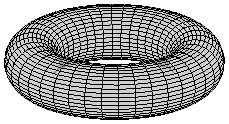
\includegraphics[width=0.9\linewidth]{figures/Torus.pdf}
\vfill
\hrulefill
\end{center}
\ \\[-5ex]
0. Auflage, \today \hfill Martin Thoma
\end{titlepage}

\chapter*{Vorwort}
Dieses Skript wird/wurde im Wintersemester 2013/2014 geschrieben.
Es beinhaltet Vorlesungsnotizen von Studenten zur Vorlesung von
Prof. Dr. Herrlich.

Es darf jeder gerne Verbesserungen einbringen!

Die Kurz-URL des Projekts lautet \href{http://tinyurl.com/GeoTopo}{tinyurl.com/GeoTopo}.

An dieser Stelle möchte ich noch Herrn Prof. Dr. Herrlich 
für einige Korrekturvorschläge und einen gut strukturierten 
Tafelanschrieb danken, der als Vorlage für dieses Skript diente.
Vielen Dank auch an Frau Lenz und Frau Randecker, die es mir erlaubt 
haben, ihre Übungsaufgaben und Lösungen zu benutzen.


\section*{Was ist Topologie?}

Die Kugeloberfläche $S^2$ lässt sich durch strecken, stauchen
und umformen zur Würfeloberfläche oder
der Oberfläche einer Pyramide verformen, aber nicht zum $\mdr^2$
oder zu einem Torus $T^2$. Für den $\mdr^2$ müsste man die Oberfläche
unendlich ausdehnen und für einen Torus müsste man ein Loch machen.

\begin{figure}[ht]
    \centering
    \subfloat[$S^2$]{
        % Source: http://tex.stackexchange.com/a/42865/5645
\begin{tikzpicture}
    \draw (-1,0) arc (180:360:1cm and 0.5cm);
    \draw[dashed] (-1,0) arc (180:0:1cm and 0.5cm);
    \draw (0,1) arc (90:270:0.5cm and 1cm);
    \draw[dashed] (0,1) arc (90:-90:0.5cm and 1cm);
    \draw (0,0) circle (1cm);
    \shade[ball color=blue!10!white,opacity=0.20] (0,0) circle (1cm);
\end{tikzpicture}

        \label{fig:s2}
    }%
    \subfloat[Würfel]{
        % Source: http://tex.stackexchange.com/a/12069/5645
\begin{tikzpicture}[scale=0.5]
   \clip (-3,-3) rectangle (3,3);
   \coordinate (tf) at (0,0);
   \coordinate (bf) at (0,-3);
   \coordinate (tr) at (15:2.5cm);
   \coordinate (tl) at (165:2.5cm);

   % You can change the perspective by playing with the 5, 5, 15:
   \coordinate (fr) at ($ (tf)!5!(tr) $);
   \coordinate (fl) at ($ (tf)!5!(tl) $);
   \coordinate (fb) at ($ (tf)!15!(bf) $);

   \path[name path=brpath] (bf) -- (fr);
   \path[name path=rbpath] (tr) -- (fb);
   \path[name path=blpath] (bf) -- (fl);
   \path[name path=lbpath] (tl) -- (fb);
   \path[name path=trpath] (tl) -- (fr);
   \path[name path=tlpath] (tr) -- (fl);

   \draw[name intersections={of=brpath and rbpath}] (intersection-1)coordinate (br){}; 
   \draw[name intersections={of=blpath and lbpath}] (intersection-1)coordinate (bl){}; 
   \draw[name intersections={of=trpath and tlpath}] (intersection-1)coordinate (tb){}; 

   \shade[right color=gray!10, left color=black!50, shading angle=105] (tf) -- (bf) -- (bl) -- (tl) -- cycle;
   \shade[left color=gray!10, right color=black!50, shading angle=75] (tf) -- (bf) -- (br) -- (tr) -- cycle;

   \begin{scope}
      \clip (tf) -- (tr) -- (tb) -- (tl) -- cycle;
      \shade[inner color = gray!5, outer color=black!50, shading=radial] (tf) ellipse (3cm and 1.5cm);
   \end{scope}

   \draw (tf) -- (bf);
   \draw (tf) -- (tr);
   \draw (tf) -- (tl);
   \draw (tr) -- (br);
   \draw (bf) -- (br);
   \draw (tl) -- (bl);
   \draw (bf) -- (bl);
   \draw (tb) -- (tr);
   \draw (tb) -- (tl);

   %set the sizes of the little cubes:
   \def\tone{.4}\def\ttwo{.75}\def\fone{.36}\def\ftwo{.70}
   \draw ($ (bf)!\tone!(br) $) -- ($ (tf)!\tone!(tr) $) -- ($ (tl)!\tone!(tb) $);
   \draw ($ (bf)!\ttwo!(br) $) -- ($ (tf)!\ttwo!(tr) $) -- ($ (tl)!\ttwo!(tb) $);
   \draw ($ (bf)!\tone!(bl) $) -- ($ (tf)!\tone!(tl) $) -- ($ (tr)!\tone!(tb) $);
   \draw ($ (bf)!\ttwo!(bl) $) -- ($ (tf)!\ttwo!(tl) $) -- ($ (tr)!\ttwo!(tb) $);
   \draw ($ (tl)!\fone!(bl) $) -- ($ (tf)!\fone!(bf) $) -- ($ (tr)!\fone!(br) $);
   \draw ($ (tl)!\ftwo!(bl) $) -- ($ (tf)!\ftwo!(bf) $) -- ($ (tr)!\ftwo!(br) $);
\end{tikzpicture}

        \label{fig:cube}
    }%
    \subfloat[Pyramide]{
        \begin{tikzpicture}[scale=.5, z={(.707,.3)}]
    \draw (2,3,2) -- (0,0,0) -- (4,0,0) -- (4,0,4) -- (2,3,2) 
      -- (4,0,0);
    \draw[color=gray, style=dashed] (2,3,2) -- (0,0,4) 
      -- (0,0,0);
    \draw[color=gray, style=dashed] (0,0,4) -- (4,0,4);
  \end{tikzpicture}

        \label{fig:pyramide}
    }

    \subfloat[$\mdr^2$]{
        \documentclass[varwidth=true, border=2pt]{standalone}
\usepackage{tikz}
\usepackage{tikz-3dplot}

\begin{document}
\tdplotsetmaincoords{110}{50}
\begin{tikzpicture}
		[tdplot_main_coords,
			cube/.style={very thick,black},
			grid/.style={very thin,gray},
			axis/.style={->,blue,thick}]

	%draw a grid in the x-y plane
	\foreach \x in {-0.5,0,...,2.5}
		\foreach \y in {-0.5,0,...,2.5}
		{
			\draw[grid] (\x,-0.5) -- (\x,2.5);
			\draw[grid] (-0.5,\y) -- (2.5,\y);
		}
			

	%draw the axes
	\draw[axis] (-1,0,0) -- (3,0,0) node[anchor=west]{$y$};
	\draw[axis] (0,-1,0) -- (0,3,0) node[anchor=west]{$x$};
	
\end{tikzpicture}
\end{document}

        \label{fig:plane-r2}
    }%
    \subfloat[$T^2$]{
        % Sketch output, version 0.3 (build 7d, Wed May 2 04:54:35 2012)
% Output language: PGF/TikZ,LaTeX
\begin{tikzpicture}[line join=round]
\filldraw[draw=black,fill=lightgray,fill opacity=0.75](-.048,.046)--(-.05,.045)--(.146,.042)--(.138,.044)--cycle;
\filldraw[draw=black,fill=lightgray,fill opacity=0.75](-.232,.038)--(-.246,.036)--(-.05,.045)--(-.048,.046)--cycle;
\filldraw[draw=black,fill=lightgray,fill opacity=0.75](.138,.044)--(.146,.042)--(.339,.028)--(.32,.031)--cycle;
\filldraw[draw=black,fill=lightgray,fill opacity=0.75](-.411,.02)--(-.435,.017)--(-.246,.036)--(-.232,.038)--cycle;
\filldraw[draw=black,fill=lightgray,fill opacity=0.75](.435,.951)--(.417,.954)--(.643,.923)--(.672,.919)--cycle;
\filldraw[draw=black,fill=lightgray,fill opacity=0.75](-.302,.964)--(-.288,.954)--(-.059,.964)--(-.062,.974)--cycle;
\filldraw[draw=black,fill=lightgray,fill opacity=0.75](-.062,.974)--(-.059,.964)--(.171,.961)--(.179,.971)--cycle;
\filldraw[draw=black,fill=lightgray,fill opacity=0.75](.179,.971)--(.171,.961)--(.397,.944)--(.417,.954)--cycle;
\filldraw[draw=black,fill=lightgray,fill opacity=0.75](-.045,.059)--(-.048,.046)--(.138,.044)--(.131,.057)--cycle;
\filldraw[draw=black,fill=lightgray,fill opacity=0.75](-.22,.051)--(-.232,.038)--(-.048,.046)--(-.045,.059)--cycle;
\filldraw[draw=black,fill=lightgray,fill opacity=0.75](-.787,.898)--(-.754,.903)--(-.535,.94)--(-.558,.937)--cycle;
\filldraw[draw=black,fill=lightgray,fill opacity=0.75](.131,.057)--(.138,.044)--(.32,.031)--(.304,.044)--cycle;
\filldraw[draw=black,fill=lightgray,fill opacity=0.75](-.535,.94)--(-.51,.931)--(-.288,.954)--(-.302,.964)--cycle;
\filldraw[draw=black,fill=lightgray,fill opacity=0.75](-.39,.034)--(-.411,.02)--(-.232,.038)--(-.22,.051)--cycle;
\filldraw[draw=black,fill=lightgray,fill opacity=0.75](.417,.954)--(.397,.944)--(.614,.915)--(.643,.923)--cycle;
\filldraw[draw=black,fill=lightgray,fill opacity=0.75](.304,.044)--(.32,.031)--(.495,.007)--(.469,.022)--cycle;
\filldraw[draw=black,fill=lightgray,fill opacity=0.75](.672,.919)--(.643,.923)--(.854,.88)--(.892,.875)--cycle;
\filldraw[draw=black,fill=lightgray,fill opacity=0.75](-.059,.964)--(-.056,.943)--(.163,.94)--(.171,.961)--cycle;
\filldraw[draw=black,fill=lightgray,fill opacity=0.75](-.288,.954)--(-.274,.933)--(-.056,.943)--(-.059,.964)--cycle;
\filldraw[draw=black,fill=lightgray,fill opacity=0.75](.171,.961)--(.163,.94)--(.378,.924)--(.397,.944)--cycle;
\filldraw[draw=black,fill=lightgray,fill opacity=0.75](-.55,.007)--(-.58,-.009)--(-.411,.02)--(-.39,.034)--cycle;
\filldraw[draw=black,fill=lightgray,fill opacity=0.75](-.754,.903)--(-.719,.896)--(-.51,.931)--(-.535,.94)--cycle;
\filldraw[draw=black,fill=lightgray,fill opacity=0.75](-.209,.076)--(-.22,.051)--(-.045,.059)--(-.043,.083)--cycle;
\filldraw[draw=black,fill=lightgray,fill opacity=0.75](-.043,.083)--(-.045,.059)--(.131,.057)--(.124,.081)--cycle;
\filldraw[draw=black,fill=lightgray,fill opacity=0.75](.124,.081)--(.131,.057)--(.304,.044)--(.289,.069)--cycle;
\filldraw[draw=black,fill=lightgray,fill opacity=0.75](-.51,.931)--(-.485,.912)--(-.274,.933)--(-.288,.954)--cycle;
\filldraw[draw=black,fill=lightgray,fill opacity=0.75](-.37,.059)--(-.39,.034)--(-.22,.051)--(-.209,.076)--cycle;
\filldraw[draw=black,fill=lightgray,fill opacity=0.75](.469,.022)--(.495,.007)--(.657,-.026)--(.623,-.009)--cycle;
\filldraw[draw=black,fill=lightgray,fill opacity=0.75](-.997,.847)--(-.955,.853)--(-.754,.903)--(-.787,.898)--cycle;
\filldraw[draw=black,fill=lightgray,fill opacity=0.75](.397,.944)--(.378,.924)--(.583,.897)--(.614,.915)--cycle;
\filldraw[draw=black,fill=lightgray,fill opacity=0.75](.289,.069)--(.304,.044)--(.469,.022)--(.446,.048)--cycle;
\filldraw[draw=black,fill=lightgray,fill opacity=0.75](.643,.923)--(.614,.915)--(.815,.874)--(.854,.88)--cycle;
\filldraw[draw=black,fill=lightgray,fill opacity=0.75](-.056,.943)--(-.053,.911)--(.154,.908)--(.163,.94)--cycle;
\filldraw[draw=black,fill=lightgray,fill opacity=0.75](-.274,.933)--(-.26,.902)--(-.053,.911)--(-.056,.943)--cycle;
\filldraw[draw=black,fill=lightgray,fill opacity=0.75](.163,.94)--(.154,.908)--(.358,.893)--(.378,.924)--cycle;
\filldraw[draw=black,fill=lightgray,fill opacity=0.75](-.522,.033)--(-.55,.007)--(-.39,.034)--(-.37,.059)--cycle;
\filldraw[draw=black,fill=lightgray,fill opacity=0.75](-.719,.896)--(-.684,.878)--(-.485,.912)--(-.51,.931)--cycle;
\filldraw[draw=black,fill=lightgray,fill opacity=0.75](-.696,-.029)--(-.735,-.047)--(-.58,-.009)--(-.55,.007)--cycle;
\filldraw[draw=black,fill=lightgray,fill opacity=0.75](-.2,.11)--(-.209,.076)--(-.043,.083)--(-.041,.117)--cycle;
\filldraw[draw=black,fill=lightgray,fill opacity=0.75](-.041,.117)--(-.043,.083)--(.124,.081)--(.119,.115)--cycle;
\filldraw[draw=black,fill=lightgray,fill opacity=0.75](.119,.115)--(.124,.081)--(.289,.069)--(.276,.104)--cycle;
\filldraw[draw=black,fill=lightgray,fill opacity=0.75](-.485,.912)--(-.459,.881)--(-.26,.902)--(-.274,.933)--cycle;
\filldraw[draw=black,fill=lightgray,fill opacity=0.75](-.354,.095)--(-.37,.059)--(-.209,.076)--(-.2,.11)--cycle;
\filldraw[draw=black,fill=lightgray,fill opacity=0.75](.892,.875)--(.854,.88)--(1.044,.826)--(1.09,.818)--cycle;
\filldraw[draw=black,fill=lightgray,fill opacity=0.75](-.955,.853)--(-.911,.849)--(-.719,.896)--(-.754,.903)--cycle;
\filldraw[draw=black,fill=lightgray,fill opacity=0.75](.446,.048)--(.469,.022)--(.623,-.009)--(.592,.018)--cycle;
\filldraw[draw=black,fill=lightgray,fill opacity=0.75](.378,.924)--(.358,.893)--(.553,.867)--(.583,.897)--cycle;
\filldraw[draw=black,fill=lightgray,fill opacity=0.75](.276,.104)--(.289,.069)--(.446,.048)--(.426,.084)--cycle;
\filldraw[draw=black,fill=lightgray,fill opacity=0.75](.614,.915)--(.583,.897)--(.775,.858)--(.815,.874)--cycle;
\filldraw[draw=black,fill=lightgray,fill opacity=0.75](.623,-.009)--(.657,-.026)--(.804,-.068)--(.761,-.049)--cycle;
\filldraw[draw=black,fill=lightgray,fill opacity=0.75](-.053,.911)--(-.05,.869)--(.146,.866)--(.154,.908)--cycle;
\filldraw[draw=black,fill=lightgray,fill opacity=0.75](-.26,.902)--(-.246,.861)--(-.05,.869)--(-.053,.911)--cycle;
\filldraw[draw=black,fill=lightgray,fill opacity=0.75](.154,.908)--(.146,.866)--(.339,.852)--(.358,.893)--cycle;
\filldraw[draw=black,fill=lightgray,fill opacity=0.75](-.499,.07)--(-.522,.033)--(-.37,.059)--(-.354,.095)--cycle;
\filldraw[draw=black,fill=lightgray,fill opacity=0.75](-.684,.878)--(-.648,.849)--(-.459,.881)--(-.485,.912)--cycle;
\filldraw[draw=black,fill=lightgray,fill opacity=0.75](-.662,-.001)--(-.696,-.029)--(-.55,.007)--(-.522,.033)--cycle;
\filldraw[draw=black,fill=lightgray,fill opacity=0.75](-.04,.161)--(-.041,.117)--(.119,.115)--(.114,.159)--cycle;
\filldraw[draw=black,fill=lightgray,fill opacity=0.75](-.193,.155)--(-.2,.11)--(-.041,.117)--(-.04,.161)--cycle;
\filldraw[draw=black,fill=lightgray,fill opacity=0.75](.114,.159)--(.119,.115)--(.276,.104)--(.265,.148)--cycle;
\filldraw[draw=black,fill=lightgray,fill opacity=0.75](-.459,.881)--(-.435,.841)--(-.246,.861)--(-.26,.902)--cycle;
\filldraw[draw=black,fill=lightgray,fill opacity=0.75](.854,.88)--(.815,.874)--(.996,.822)--(1.044,.826)--cycle;
\filldraw[draw=black,fill=lightgray,fill opacity=0.75](-.341,.139)--(-.354,.095)--(-.2,.11)--(-.193,.155)--cycle;
\filldraw[draw=black,fill=lightgray,fill opacity=0.75](-.911,.849)--(-.866,.833)--(-.684,.878)--(-.719,.896)--cycle;
\filldraw[draw=black,fill=lightgray,fill opacity=0.75](-1.182,.784)--(-1.132,.793)--(-.955,.853)--(-.997,.847)--cycle;
\filldraw[draw=black,fill=lightgray,fill opacity=0.75](.426,.084)--(.446,.048)--(.592,.018)--(.566,.055)--cycle;
\filldraw[draw=black,fill=lightgray,fill opacity=0.75](.358,.893)--(.339,.852)--(.523,.828)--(.553,.867)--cycle;
\filldraw[draw=black,fill=lightgray,fill opacity=0.75](-.825,-.073)--(-.871,-.093)--(-.735,-.047)--(-.696,-.029)--cycle;
\filldraw[draw=black,fill=lightgray,fill opacity=0.75](.265,.148)--(.276,.104)--(.426,.084)--(.41,.129)--cycle;
\filldraw[draw=black,fill=lightgray,fill opacity=0.75](.583,.897)--(.553,.867)--(.734,.83)--(.775,.858)--cycle;
\filldraw[draw=black,fill=lightgray,fill opacity=0.75](.592,.018)--(.623,-.009)--(.761,-.049)--(.724,-.02)--cycle;
\filldraw[draw=black,fill=lightgray,fill opacity=0.75](-.05,.869)--(-.048,.818)--(.138,.816)--(.146,.866)--cycle;
\filldraw[draw=black,fill=lightgray,fill opacity=0.75](-.246,.861)--(-.232,.81)--(-.048,.818)--(-.05,.869)--cycle;
\filldraw[draw=black,fill=lightgray,fill opacity=0.75](.146,.866)--(.138,.816)--(.32,.803)--(.339,.852)--cycle;
\filldraw[draw=black,fill=lightgray,fill opacity=0.75](-.038,.214)--(-.04,.161)--(.114,.159)--(.111,.212)--cycle;
\filldraw[draw=black,fill=lightgray,fill opacity=0.75](-.187,.208)--(-.193,.155)--(-.04,.161)--(-.038,.214)--cycle;
\filldraw[draw=black,fill=lightgray,fill opacity=0.75](-.481,.116)--(-.499,.07)--(-.354,.095)--(-.341,.139)--cycle;
\filldraw[draw=black,fill=lightgray,fill opacity=0.75](-.648,.849)--(-.613,.811)--(-.435,.841)--(-.459,.881)--cycle;
\filldraw[draw=black,fill=lightgray,fill opacity=0.75](-.632,.038)--(-.662,-.001)--(-.522,.033)--(-.499,.07)--cycle;
\filldraw[draw=black,fill=lightgray,fill opacity=0.75](.111,.212)--(.114,.159)--(.265,.148)--(.258,.201)--cycle;
\filldraw[draw=black,fill=lightgray,fill opacity=0.75](-.435,.841)--(-.411,.792)--(-.232,.81)--(-.246,.861)--cycle;
\filldraw[draw=black,fill=lightgray,fill opacity=0.75](-.331,.193)--(-.341,.139)--(-.193,.155)--(-.187,.208)--cycle;
\filldraw[draw=black,fill=lightgray,fill opacity=0.75](.815,.874)--(.775,.858)--(.947,.808)--(.996,.822)--cycle;
\filldraw[draw=black,fill=lightgray,fill opacity=0.75](-.866,.833)--(-.821,.807)--(-.648,.849)--(-.684,.878)--cycle;
\filldraw[draw=black,fill=lightgray,fill opacity=0.75](-1.132,.793)--(-1.08,.792)--(-.911,.849)--(-.955,.853)--cycle;
\filldraw[draw=black,fill=lightgray,fill opacity=0.75](.41,.129)--(.426,.084)--(.566,.055)--(.545,.102)--cycle;
\filldraw[draw=black,fill=lightgray,fill opacity=0.75](.761,-.049)--(.804,-.068)--(.93,-.118)--(.881,-.096)--cycle;
\filldraw[draw=black,fill=lightgray,fill opacity=0.75](.339,.852)--(.32,.803)--(.495,.779)--(.523,.828)--cycle;
\filldraw[draw=black,fill=lightgray,fill opacity=0.75](-.784,-.042)--(-.825,-.073)--(-.696,-.029)--(-.662,-.001)--cycle;
\filldraw[draw=black,fill=lightgray,fill opacity=0.75](.258,.201)--(.265,.148)--(.41,.129)--(.398,.183)--cycle;
\filldraw[draw=black,fill=lightgray,fill opacity=0.75](.553,.867)--(.523,.828)--(.695,.793)--(.734,.83)--cycle;
\filldraw[draw=black,fill=lightgray,fill opacity=0.75](-.048,.818)--(-.045,.76)--(.131,.758)--(.138,.816)--cycle;
\filldraw[draw=black,fill=lightgray,fill opacity=0.75](-.232,.81)--(-.22,.753)--(-.045,.76)--(-.048,.818)--cycle;
\filldraw[draw=black,fill=lightgray,fill opacity=0.75](1.09,.818)--(1.044,.826)--(1.209,.761)--(1.262,.75)--cycle;
\filldraw[draw=black,fill=lightgray,fill opacity=0.75](.566,.055)--(.592,.018)--(.724,-.02)--(.691,.019)--cycle;
\filldraw[draw=black,fill=lightgray,fill opacity=0.75](.138,.816)--(.131,.758)--(.304,.745)--(.32,.803)--cycle;
\filldraw[draw=black,fill=lightgray,fill opacity=0.75](-.038,.274)--(-.038,.214)--(.111,.212)--(.109,.272)--cycle;
\filldraw[draw=black,fill=lightgray,fill opacity=0.75](-.184,.268)--(-.187,.208)--(-.038,.214)--(-.038,.274)--cycle;
\filldraw[draw=black,fill=lightgray,fill opacity=0.75](.109,.272)--(.111,.212)--(.258,.201)--(.253,.261)--cycle;
\filldraw[draw=black,fill=lightgray,fill opacity=0.75](-.467,.17)--(-.481,.116)--(-.341,.139)--(-.331,.193)--cycle;
\filldraw[draw=black,fill=lightgray,fill opacity=0.75](-.613,.811)--(-.58,.763)--(-.411,.792)--(-.435,.841)--cycle;
\filldraw[draw=black,fill=lightgray,fill opacity=0.75](-.411,.792)--(-.39,.735)--(-.22,.753)--(-.232,.81)--cycle;
\filldraw[draw=black,fill=lightgray,fill opacity=0.75](-.609,.085)--(-.632,.038)--(-.499,.07)--(-.481,.116)--cycle;
\filldraw[draw=black,fill=lightgray,fill opacity=0.75](-.325,.253)--(-.331,.193)--(-.187,.208)--(-.184,.268)--cycle;
\filldraw[draw=black,fill=lightgray,fill opacity=0.75](-1.39,.689)--(-1.338,.712)--(-1.182,.784)--(-1.228,.764)--cycle;
\filldraw[draw=black,fill=lightgray,fill opacity=0.75](.775,.858)--(.734,.83)--(.897,.783)--(.947,.808)--cycle;
\filldraw[draw=black,fill=lightgray,fill opacity=0.75](.32,.803)--(.304,.745)--(.469,.723)--(.495,.779)--cycle;
\filldraw[draw=black,fill=lightgray,fill opacity=0.75](.398,.183)--(.41,.129)--(.545,.102)--(.529,.156)--cycle;
\filldraw[draw=black,fill=lightgray,fill opacity=0.75](.253,.261)--(.258,.201)--(.398,.183)--(.391,.243)--cycle;
\filldraw[draw=black,fill=lightgray,fill opacity=0.75](-.045,.76)--(-.043,.696)--(.124,.693)--(.131,.758)--cycle;
\filldraw[draw=black,fill=lightgray,fill opacity=0.75](-.22,.753)--(-.209,.689)--(-.043,.696)--(-.045,.76)--cycle;
\filldraw[draw=black,fill=lightgray,fill opacity=0.75](-.821,.807)--(-.776,.771)--(-.613,.811)--(-.648,.849)--cycle;
\filldraw[draw=black,fill=lightgray,fill opacity=0.75](.724,-.02)--(.761,-.049)--(.881,-.096)--(.837,-.065)--cycle;
\filldraw[draw=black,fill=lightgray,fill opacity=0.75](-1.08,.792)--(-1.026,.779)--(-.866,.833)--(-.911,.849)--cycle;
\filldraw[draw=black,fill=lightgray,fill opacity=0.75](.131,.758)--(.124,.693)--(.289,.682)--(.304,.745)--cycle;
\filldraw[draw=black,fill=lightgray,fill opacity=0.75](-.75,-.002)--(-.784,-.042)--(-.662,-.001)--(-.632,.038)--cycle;
\filldraw[draw=black,fill=lightgray,fill opacity=0.75](-.038,.34)--(-.038,.274)--(.109,.272)--(.108,.338)--cycle;
\filldraw[draw=black,fill=lightgray,fill opacity=0.75](-.183,.333)--(-.184,.268)--(-.038,.274)--(-.038,.34)--cycle;
\filldraw[draw=black,fill=lightgray,fill opacity=0.75](.523,.828)--(.495,.779)--(.657,.746)--(.695,.793)--cycle;
\filldraw[draw=black,fill=lightgray,fill opacity=0.75](.108,.338)--(.109,.272)--(.253,.261)--(.252,.327)--cycle;
\filldraw[draw=black,fill=lightgray,fill opacity=0.75](1.044,.826)--(.996,.822)--(1.153,.761)--(1.209,.761)--cycle;
\filldraw[draw=black,fill=lightgray,fill opacity=0.75](.545,.102)--(.566,.055)--(.691,.019)--(.666,.067)--cycle;
\filldraw[draw=black,fill=lightgray,fill opacity=0.75](-.39,.735)--(-.37,.672)--(-.209,.689)--(-.22,.753)--cycle;
\filldraw[draw=black,fill=lightgray,fill opacity=0.75](-.459,.23)--(-.467,.17)--(-.331,.193)--(-.325,.253)--cycle;
\filldraw[draw=black,fill=lightgray,fill opacity=0.75](-.58,.763)--(-.55,.708)--(-.39,.735)--(-.411,.792)--cycle;
\filldraw[draw=black,fill=lightgray,fill opacity=0.75](-.323,.319)--(-.325,.253)--(-.184,.268)--(-.183,.333)--cycle;
\filldraw[draw=black,fill=lightgray,fill opacity=0.75](-.591,.139)--(-.609,.085)--(-.481,.116)--(-.467,.17)--cycle;
\filldraw[draw=black,fill=lightgray,fill opacity=0.75](-.209,.689)--(-.2,.62)--(-.041,.627)--(-.043,.696)--cycle;
\filldraw[draw=black,fill=lightgray,fill opacity=0.75](-.043,.696)--(-.041,.627)--(.119,.625)--(.124,.693)--cycle;
\filldraw[draw=black,fill=lightgray,fill opacity=0.75](.304,.745)--(.289,.682)--(.446,.661)--(.469,.723)--cycle;
\filldraw[draw=black,fill=lightgray,fill opacity=0.75](.124,.693)--(.119,.625)--(.276,.613)--(.289,.682)--cycle;
\filldraw[draw=black,fill=lightgray,fill opacity=0.75](.252,.327)--(.253,.261)--(.391,.243)--(.389,.309)--cycle;
\filldraw[draw=black,fill=lightgray,fill opacity=0.75](-.038,.41)--(-.038,.34)--(.108,.338)--(.109,.407)--cycle;
\filldraw[draw=black,fill=lightgray,fill opacity=0.75](-.184,.403)--(-.183,.333)--(-.038,.34)--(-.038,.41)--cycle;
\filldraw[draw=black,fill=lightgray,fill opacity=0.75](-1.338,.712)--(-1.282,.724)--(-1.132,.793)--(-1.182,.784)--cycle;
\filldraw[draw=black,fill=lightgray,fill opacity=0.75](.109,.407)--(.108,.338)--(.252,.327)--(.253,.397)--cycle;
\filldraw[draw=black,fill=lightgray,fill opacity=0.75](.391,.243)--(.398,.183)--(.529,.156)--(.52,.217)--cycle;
\filldraw[draw=black,fill=lightgray,fill opacity=0.75](.734,.83)--(.695,.793)--(.849,.748)--(.897,.783)--cycle;
\filldraw[draw=black,fill=lightgray,fill opacity=0.75](-.776,.771)--(-.735,.726)--(-.58,.763)--(-.613,.811)--cycle;
\filldraw[draw=black,fill=lightgray,fill opacity=0.75](-.37,.672)--(-.354,.604)--(-.2,.62)--(-.209,.689)--cycle;
\filldraw[draw=black,fill=lightgray,fill opacity=0.75](.495,.779)--(.469,.723)--(.623,.692)--(.657,.746)--cycle;
\filldraw[draw=black,fill=lightgray,fill opacity=0.75](.691,.019)--(.724,-.02)--(.837,-.065)--(.8,-.024)--cycle;
\filldraw[draw=black,fill=lightgray,fill opacity=0.75](-1.026,.779)--(-.973,.756)--(-.821,.807)--(-.866,.833)--cycle;
\filldraw[draw=black,fill=lightgray,fill opacity=0.75](-.325,.389)--(-.323,.319)--(-.183,.333)--(-.184,.403)--cycle;
\filldraw[draw=black,fill=lightgray,fill opacity=0.75](-.2,.62)--(-.193,.548)--(-.04,.555)--(-.041,.627)--cycle;
\filldraw[draw=black,fill=lightgray,fill opacity=0.75](-.041,.627)--(-.04,.555)--(.114,.553)--(.119,.625)--cycle;
\filldraw[draw=black,fill=lightgray,fill opacity=0.75](-.888,-.09)--(-.934,-.123)--(-.825,-.073)--(-.784,-.042)--cycle;
\filldraw[draw=black,fill=lightgray,fill opacity=0.75](-.722,.046)--(-.75,-.002)--(-.632,.038)--(-.609,.085)--cycle;
\filldraw[draw=black,fill=lightgray,fill opacity=0.75](-.038,.482)--(-.038,.41)--(.109,.407)--(.111,.48)--cycle;
\filldraw[draw=black,fill=lightgray,fill opacity=0.75](-.187,.475)--(-.184,.403)--(-.038,.41)--(-.038,.482)--cycle;
\filldraw[draw=black,fill=lightgray,fill opacity=0.75](-.456,.296)--(-.459,.23)--(-.325,.253)--(-.323,.319)--cycle;
\filldraw[draw=black,fill=lightgray,fill opacity=0.75](.119,.625)--(.114,.553)--(.265,.542)--(.276,.613)--cycle;
\filldraw[draw=black,fill=lightgray,fill opacity=0.75](-.55,.708)--(-.522,.646)--(-.37,.672)--(-.39,.735)--cycle;
\filldraw[draw=black,fill=lightgray,fill opacity=0.75](.111,.48)--(.109,.407)--(.253,.397)--(.258,.469)--cycle;
\filldraw[draw=black,fill=lightgray,fill opacity=0.75](.529,.156)--(.545,.102)--(.666,.067)--(.647,.122)--cycle;
\filldraw[draw=black,fill=lightgray,fill opacity=0.75](.996,.822)--(.947,.808)--(1.096,.749)--(1.153,.761)--cycle;
\filldraw[draw=black,fill=lightgray,fill opacity=0.75](.289,.682)--(.276,.613)--(.426,.593)--(.446,.661)--cycle;
\filldraw[draw=black,fill=lightgray,fill opacity=0.75](-.04,.555)--(-.038,.482)--(.111,.48)--(.114,.553)--cycle;
\filldraw[draw=black,fill=lightgray,fill opacity=0.75](-.193,.548)--(-.187,.475)--(-.038,.482)--(-.04,.555)--cycle;
\filldraw[draw=black,fill=lightgray,fill opacity=0.75](.253,.397)--(.252,.327)--(.389,.309)--(.391,.379)--cycle;
\filldraw[draw=black,fill=lightgray,fill opacity=0.75](-.354,.604)--(-.341,.533)--(-.193,.548)--(-.2,.62)--cycle;
\filldraw[draw=black,fill=lightgray,fill opacity=0.75](.114,.553)--(.111,.48)--(.258,.469)--(.265,.542)--cycle;
\filldraw[draw=black,fill=lightgray,fill opacity=0.75](-.331,.461)--(-.325,.389)--(-.184,.403)--(-.187,.475)--cycle;
\filldraw[draw=black,fill=lightgray,fill opacity=0.75](-.581,.201)--(-.591,.139)--(-.467,.17)--(-.459,.23)--cycle;
\filldraw[draw=black,fill=lightgray,fill opacity=0.75](1.31,.729)--(1.262,.75)--(1.402,.673)--(1.456,.649)--cycle;
\filldraw[draw=black,fill=lightgray,fill opacity=0.75](-.341,.533)--(-.331,.461)--(-.187,.475)--(-.193,.548)--cycle;
\filldraw[draw=black,fill=lightgray,fill opacity=0.75](.389,.309)--(.391,.243)--(.52,.217)--(.516,.283)--cycle;
\filldraw[draw=black,fill=lightgray,fill opacity=0.75](.276,.613)--(.265,.542)--(.41,.522)--(.426,.593)--cycle;
\filldraw[draw=black,fill=lightgray,fill opacity=0.75](.258,.469)--(.253,.397)--(.391,.379)--(.398,.45)--cycle;
\filldraw[draw=black,fill=lightgray,fill opacity=0.75](-.459,.366)--(-.456,.296)--(-.323,.319)--(-.325,.389)--cycle;
\filldraw[draw=black,fill=lightgray,fill opacity=0.75](.469,.723)--(.446,.661)--(.592,.631)--(.623,.692)--cycle;
\filldraw[draw=black,fill=lightgray,fill opacity=0.75](-.522,.646)--(-.499,.579)--(-.354,.604)--(-.37,.672)--cycle;
\filldraw[draw=black,fill=lightgray,fill opacity=0.75](-.735,.726)--(-.696,.672)--(-.55,.708)--(-.58,.763)--cycle;
\filldraw[draw=black,fill=lightgray,fill opacity=0.75](-1.282,.724)--(-1.222,.726)--(-1.08,.792)--(-1.132,.793)--cycle;
\filldraw[draw=black,fill=lightgray,fill opacity=0.75](.695,.793)--(.657,.746)--(.804,.704)--(.849,.748)--cycle;
\filldraw[draw=black,fill=lightgray,fill opacity=0.75](.265,.542)--(.258,.469)--(.398,.45)--(.41,.522)--cycle;
\filldraw[draw=black,fill=lightgray,fill opacity=0.75](-.973,.756)--(-.921,.722)--(-.776,.771)--(-.821,.807)--cycle;
\filldraw[draw=black,fill=lightgray,fill opacity=0.75](.666,.067)--(.691,.019)--(.8,-.024)--(.77,.025)--cycle;
\filldraw[draw=black,fill=lightgray,fill opacity=0.75](-.701,.102)--(-.722,.046)--(-.609,.085)--(-.591,.139)--cycle;
\filldraw[draw=black,fill=lightgray,fill opacity=0.75](-.849,-.048)--(-.888,-.09)--(-.784,-.042)--(-.75,-.002)--cycle;
\filldraw[draw=black,fill=lightgray,fill opacity=0.75](.52,.217)--(.529,.156)--(.647,.122)--(.635,.184)--cycle;
\filldraw[draw=black,fill=lightgray,fill opacity=0.75](-.467,.438)--(-.459,.366)--(-.325,.389)--(-.331,.461)--cycle;
\filldraw[draw=black,fill=lightgray,fill opacity=0.75](-.499,.579)--(-.481,.509)--(-.341,.533)--(-.354,.604)--cycle;
\filldraw[draw=black,fill=lightgray,fill opacity=0.75](.391,.379)--(.389,.309)--(.516,.283)--(.52,.352)--cycle;
\filldraw[draw=black,fill=lightgray,fill opacity=0.75](-.577,.267)--(-.581,.201)--(-.459,.23)--(-.456,.296)--cycle;
\filldraw[draw=black,fill=lightgray,fill opacity=0.75](.947,.808)--(.897,.783)--(1.039,.728)--(1.096,.749)--cycle;
\filldraw[draw=black,fill=lightgray,fill opacity=0.75](.837,-.065)--(.881,-.096)--(.979,-.15)--(.931,-.116)--cycle;
\filldraw[draw=black,fill=lightgray,fill opacity=0.75](.446,.661)--(.426,.593)--(.566,.565)--(.592,.631)--cycle;
\filldraw[draw=black,fill=lightgray,fill opacity=0.75](-.481,.509)--(-.467,.438)--(-.331,.461)--(-.341,.533)--cycle;
\filldraw[draw=black,fill=lightgray,fill opacity=0.75](1.262,.75)--(1.209,.761)--(1.343,.687)--(1.402,.673)--cycle;
\filldraw[draw=black,fill=lightgray,fill opacity=0.75](-.696,.672)--(-.662,.612)--(-.522,.646)--(-.55,.708)--cycle;
\filldraw[draw=black,fill=lightgray,fill opacity=0.75](.657,.746)--(.623,.692)--(.761,.652)--(.804,.704)--cycle;
\filldraw[draw=black,fill=lightgray,fill opacity=0.75](.398,.45)--(.391,.379)--(.52,.352)--(.529,.424)--cycle;
\filldraw[draw=black,fill=lightgray,fill opacity=0.75](.426,.593)--(.41,.522)--(.545,.495)--(.566,.565)--cycle;
\filldraw[draw=black,fill=lightgray,fill opacity=0.75](-1.222,.726)--(-1.162,.716)--(-1.026,.779)--(-1.08,.792)--cycle;
\filldraw[draw=black,fill=lightgray,fill opacity=0.75](-.581,.336)--(-.577,.267)--(-.456,.296)--(-.459,.366)--cycle;
\filldraw[draw=black,fill=lightgray,fill opacity=0.75](.41,.522)--(.398,.45)--(.529,.424)--(.545,.495)--cycle;
\filldraw[draw=black,fill=lightgray,fill opacity=0.75](-.921,.722)--(-.871,.68)--(-.735,.726)--(-.776,.771)--cycle;
\filldraw[draw=black,fill=lightgray,fill opacity=0.75](.516,.283)--(.52,.217)--(.635,.184)--(.631,.25)--cycle;
\filldraw[draw=black,fill=lightgray,fill opacity=0.75](-.688,.164)--(-.701,.102)--(-.591,.139)--(-.581,.201)--cycle;
\filldraw[draw=black,fill=lightgray,fill opacity=0.75](.647,.122)--(.666,.067)--(.77,.025)--(.748,.082)--cycle;
\filldraw[draw=black,fill=lightgray,fill opacity=0.75](-.662,.612)--(-.632,.547)--(-.499,.579)--(-.522,.646)--cycle;
\filldraw[draw=black,fill=lightgray,fill opacity=0.75](-.817,.002)--(-.849,-.048)--(-.75,-.002)--(-.722,.046)--cycle;
\filldraw[draw=black,fill=lightgray,fill opacity=0.75](.897,.783)--(.849,.748)--(.983,.696)--(1.039,.728)--cycle;
\filldraw[draw=black,fill=lightgray,fill opacity=0.75](.8,-.024)--(.837,-.065)--(.931,-.116)--(.889,-.072)--cycle;
\filldraw[draw=black,fill=lightgray,fill opacity=0.75](-.591,.407)--(-.581,.336)--(-.459,.366)--(-.467,.438)--cycle;
\filldraw[draw=black,fill=lightgray,fill opacity=0.75](.623,.692)--(.592,.631)--(.724,.593)--(.761,.652)--cycle;
\filldraw[draw=black,fill=lightgray,fill opacity=0.75](-.632,.547)--(-.609,.478)--(-.481,.509)--(-.499,.579)--cycle;
\filldraw[draw=black,fill=lightgray,fill opacity=0.75](1.209,.761)--(1.153,.761)--(1.281,.691)--(1.343,.687)--cycle;
\filldraw[draw=black,fill=lightgray,fill opacity=0.75](-1.517,.605)--(-1.461,.631)--(-1.338,.712)--(-1.39,.689)--cycle;
\filldraw[draw=black,fill=lightgray,fill opacity=0.75](-.609,.478)--(-.591,.407)--(-.467,.438)--(-.481,.509)--cycle;
\filldraw[draw=black,fill=lightgray,fill opacity=0.75](.52,.352)--(.516,.283)--(.631,.25)--(.635,.319)--cycle;
\filldraw[draw=black,fill=lightgray,fill opacity=0.75](-.97,-.144)--(-1.02,-.179)--(-.934,-.123)--(-.888,-.09)--cycle;
\filldraw[draw=black,fill=lightgray,fill opacity=0.75](-.871,.68)--(-.825,.629)--(-.696,.672)--(-.735,.726)--cycle;
\filldraw[draw=black,fill=lightgray,fill opacity=0.75](-1.162,.716)--(-1.101,.696)--(-.973,.756)--(-1.026,.779)--cycle;
\filldraw[draw=black,fill=lightgray,fill opacity=0.75](-.684,.23)--(-.688,.164)--(-.581,.201)--(-.577,.267)--cycle;
\filldraw[draw=black,fill=lightgray,fill opacity=0.75](.592,.631)--(.566,.565)--(.691,.528)--(.724,.593)--cycle;
\filldraw[draw=black,fill=lightgray,fill opacity=0.75](.635,.184)--(.647,.122)--(.748,.082)--(.735,.144)--cycle;
\filldraw[draw=black,fill=lightgray,fill opacity=0.75](.529,.424)--(.52,.352)--(.635,.319)--(.647,.39)--cycle;
\filldraw[draw=black,fill=lightgray,fill opacity=0.75](-.794,.059)--(-.817,.002)--(-.722,.046)--(-.701,.102)--cycle;
\filldraw[draw=black,fill=lightgray,fill opacity=0.75](.849,.748)--(.804,.704)--(.93,.654)--(.983,.696)--cycle;
\filldraw[draw=black,fill=lightgray,fill opacity=0.75](.566,.565)--(.545,.495)--(.666,.46)--(.691,.528)--cycle;
\filldraw[draw=black,fill=lightgray,fill opacity=0.75](.77,.025)--(.8,-.024)--(.889,-.072)--(.856,-.021)--cycle;
\filldraw[draw=black,fill=lightgray,fill opacity=0.75](.545,.495)--(.529,.424)--(.647,.39)--(.666,.46)--cycle;
\filldraw[draw=black,fill=lightgray,fill opacity=0.75](-.825,.629)--(-.784,.571)--(-.662,.612)--(-.696,.672)--cycle;
\filldraw[draw=black,fill=lightgray,fill opacity=0.75](-.688,.3)--(-.684,.23)--(-.577,.267)--(-.581,.336)--cycle;
\filldraw[draw=black,fill=lightgray,fill opacity=0.75](1.153,.761)--(1.096,.749)--(1.218,.683)--(1.281,.691)--cycle;
\filldraw[draw=black,fill=lightgray,fill opacity=0.75](-1.461,.631)--(-1.399,.647)--(-1.282,.724)--(-1.338,.712)--cycle;
\filldraw[draw=black,fill=lightgray,fill opacity=0.75](-.927,-.099)--(-.97,-.144)--(-.888,-.09)--(-.849,-.048)--cycle;
\filldraw[draw=black,fill=lightgray,fill opacity=0.75](-1.101,.696)--(-1.042,.666)--(-.921,.722)--(-.973,.756)--cycle;
\filldraw[draw=black,fill=lightgray,fill opacity=0.75](.631,.25)--(.635,.184)--(.735,.144)--(.73,.211)--cycle;
\filldraw[draw=black,fill=lightgray,fill opacity=0.75](1.505,.615)--(1.456,.649)--(1.566,.562)--(1.618,.525)--cycle;
\filldraw[draw=black,fill=lightgray,fill opacity=0.75](.804,.704)--(.761,.652)--(.881,.605)--(.93,.654)--cycle;
\filldraw[draw=black,fill=lightgray,fill opacity=0.75](-.784,.571)--(-.75,.507)--(-.632,.547)--(-.662,.612)--cycle;
\filldraw[draw=black,fill=lightgray,fill opacity=0.75](-.701,.37)--(-.688,.3)--(-.581,.336)--(-.591,.407)--cycle;
\filldraw[draw=black,fill=lightgray,fill opacity=0.75](-.779,.122)--(-.794,.059)--(-.701,.102)--(-.688,.164)--cycle;
\filldraw[draw=black,fill=lightgray,fill opacity=0.75](-.75,.507)--(-.722,.44)--(-.609,.478)--(-.632,.547)--cycle;
\filldraw[draw=black,fill=lightgray,fill opacity=0.75](-.722,.44)--(-.701,.37)--(-.591,.407)--(-.609,.478)--cycle;
\filldraw[draw=black,fill=lightgray,fill opacity=0.75](.748,.082)--(.77,.025)--(.856,-.021)--(.832,.037)--cycle;
\filldraw[draw=black,fill=lightgray,fill opacity=0.75](.635,.319)--(.631,.25)--(.73,.211)--(.735,.28)--cycle;
\filldraw[draw=black,fill=lightgray,fill opacity=0.75](1.096,.749)--(1.039,.728)--(1.154,.665)--(1.218,.683)--cycle;
\filldraw[draw=black,fill=lightgray,fill opacity=0.75](-1.399,.647)--(-1.335,.652)--(-1.222,.726)--(-1.282,.724)--cycle;
\filldraw[draw=black,fill=lightgray,fill opacity=0.75](.761,.652)--(.724,.593)--(.837,.548)--(.881,.605)--cycle;
\filldraw[draw=black,fill=lightgray,fill opacity=0.75](-1.042,.666)--(-.986,.626)--(-.871,.68)--(-.921,.722)--cycle;
\filldraw[draw=black,fill=lightgray,fill opacity=0.75](-.892,-.047)--(-.927,-.099)--(-.849,-.048)--(-.817,.002)--cycle;
\filldraw[draw=black,fill=lightgray,fill opacity=0.75](1.456,.649)--(1.402,.673)--(1.508,.59)--(1.566,.562)--cycle;
\filldraw[draw=black,fill=lightgray,fill opacity=0.75](-.775,.189)--(-.779,.122)--(-.688,.164)--(-.684,.23)--cycle;
\filldraw[draw=black,fill=lightgray,fill opacity=0.75](.647,.39)--(.635,.319)--(.735,.28)--(.748,.35)--cycle;
\filldraw[draw=black,fill=lightgray,fill opacity=0.75](.724,.593)--(.691,.528)--(.8,.486)--(.837,.548)--cycle;
\filldraw[draw=black,fill=lightgray,fill opacity=0.75](.889,-.072)--(.931,-.116)--(1.001,-.171)--(.956,-.125)--cycle;
\filldraw[draw=black,fill=lightgray,fill opacity=0.75](.735,.144)--(.748,.082)--(.832,.037)--(.817,.1)--cycle;
\filldraw[draw=black,fill=lightgray,fill opacity=0.75](.666,.46)--(.647,.39)--(.748,.35)--(.77,.419)--cycle;
\filldraw[draw=black,fill=lightgray,fill opacity=0.75](.691,.528)--(.666,.46)--(.77,.419)--(.8,.486)--cycle;
\filldraw[draw=black,fill=lightgray,fill opacity=0.75](-.986,.626)--(-.934,.578)--(-.825,.629)--(-.871,.68)--cycle;
\filldraw[draw=black,fill=lightgray,fill opacity=0.75](1.039,.728)--(.983,.696)--(1.092,.636)--(1.154,.665)--cycle;
\filldraw[draw=black,fill=lightgray,fill opacity=0.75](-1.335,.652)--(-1.269,.646)--(-1.162,.716)--(-1.222,.726)--cycle;
\filldraw[draw=black,fill=lightgray,fill opacity=0.75](-.779,.258)--(-.775,.189)--(-.684,.23)--(-.688,.3)--cycle;
\filldraw[draw=black,fill=lightgray,fill opacity=0.75](-.867,.012)--(-.892,-.047)--(-.817,.002)--(-.794,.059)--cycle;
\filldraw[draw=black,fill=lightgray,fill opacity=0.75](1.402,.673)--(1.343,.687)--(1.445,.607)--(1.508,.59)--cycle;
\filldraw[draw=black,fill=lightgray,fill opacity=0.75](-.934,.578)--(-.888,.523)--(-.784,.571)--(-.825,.629)--cycle;
\filldraw[draw=black,fill=lightgray,fill opacity=0.75](.73,.211)--(.735,.144)--(.817,.1)--(.812,.166)--cycle;
\filldraw[draw=black,fill=lightgray,fill opacity=0.75](.856,-.021)--(.889,-.072)--(.956,-.125)--(.921,-.072)--cycle;
\filldraw[draw=black,fill=lightgray,fill opacity=0.75](-.794,.327)--(-.779,.258)--(-.688,.3)--(-.701,.37)--cycle;
\filldraw[draw=black,fill=lightgray,fill opacity=0.75](.983,.696)--(.93,.654)--(1.033,.598)--(1.092,.636)--cycle;
\filldraw[draw=black,fill=lightgray,fill opacity=0.75](-.888,.523)--(-.849,.461)--(-.75,.507)--(-.784,.571)--cycle;
\filldraw[draw=black,fill=lightgray,fill opacity=0.75](-1.269,.646)--(-1.203,.63)--(-1.101,.696)--(-1.162,.716)--cycle;
\filldraw[draw=black,fill=lightgray,fill opacity=0.75](-1.661,.477)--(-1.608,.515)--(-1.517,.605)--(-1.568,.57)--cycle;
\filldraw[draw=black,fill=lightgray,fill opacity=0.75](-.817,.396)--(-.794,.327)--(-.701,.37)--(-.722,.44)--cycle;
\filldraw[draw=black,fill=lightgray,fill opacity=0.75](-.851,.075)--(-.867,.012)--(-.794,.059)--(-.779,.122)--cycle;
\filldraw[draw=black,fill=lightgray,fill opacity=0.75](-.849,.461)--(-.817,.396)--(-.722,.44)--(-.75,.507)--cycle;
\filldraw[draw=black,fill=lightgray,fill opacity=0.75](1.343,.687)--(1.281,.691)--(1.378,.614)--(1.445,.607)--cycle;
\filldraw[draw=black,fill=lightgray,fill opacity=0.75](.735,.28)--(.73,.211)--(.812,.166)--(.817,.235)--cycle;
\filldraw[draw=black,fill=lightgray,fill opacity=0.75](-.982,-.154)--(-1.028,-.201)--(-.97,-.144)--(-.927,-.099)--cycle;
\filldraw[draw=black,fill=lightgray,fill opacity=0.75](.93,.654)--(.881,.605)--(.979,.551)--(1.033,.598)--cycle;
\filldraw[draw=black,fill=lightgray,fill opacity=0.75](.832,.037)--(.856,-.021)--(.921,-.072)--(.894,-.013)--cycle;
\filldraw[draw=black,fill=lightgray,fill opacity=0.75](-1.203,.63)--(-1.138,.603)--(-1.042,.666)--(-1.101,.696)--cycle;
\filldraw[draw=black,fill=lightgray,fill opacity=0.75](.748,.35)--(.735,.28)--(.817,.235)--(.832,.304)--cycle;
\filldraw[draw=black,fill=lightgray,fill opacity=0.75](-1.608,.515)--(-1.548,.545)--(-1.461,.631)--(-1.517,.605)--cycle;
\filldraw[draw=black,fill=lightgray,fill opacity=0.75](.881,.605)--(.837,.548)--(.931,.497)--(.979,.551)--cycle;
\filldraw[draw=black,fill=lightgray,fill opacity=0.75](-.846,.142)--(-.851,.075)--(-.779,.122)--(-.775,.189)--cycle;
\filldraw[draw=black,fill=lightgray,fill opacity=0.75](1.281,.691)--(1.218,.683)--(1.31,.61)--(1.378,.614)--cycle;
\filldraw[draw=black,fill=lightgray,fill opacity=0.75](.77,.419)--(.748,.35)--(.832,.304)--(.856,.372)--cycle;
\filldraw[draw=black,fill=lightgray,fill opacity=0.75](-.945,-.1)--(-.982,-.154)--(-.927,-.099)--(-.892,-.047)--cycle;
\filldraw[draw=black,fill=lightgray,fill opacity=0.75](.837,.548)--(.8,.486)--(.889,.437)--(.931,.497)--cycle;
\filldraw[draw=black,fill=lightgray,fill opacity=0.75](.8,.486)--(.77,.419)--(.856,.372)--(.889,.437)--cycle;
\filldraw[draw=black,fill=lightgray,fill opacity=0.75](.817,.1)--(.832,.037)--(.894,-.013)--(.878,.051)--cycle;
\filldraw[draw=black,fill=lightgray,fill opacity=0.75](-1.138,.603)--(-1.077,.567)--(-.986,.626)--(-1.042,.666)--cycle;
\filldraw[draw=black,fill=lightgray,fill opacity=0.75](-.851,.211)--(-.846,.142)--(-.775,.189)--(-.779,.258)--cycle;
\filldraw[draw=black,fill=lightgray,fill opacity=0.75](-1.548,.545)--(-1.483,.564)--(-1.399,.647)--(-1.461,.631)--cycle;
\filldraw[draw=black,fill=lightgray,fill opacity=0.75](1.663,.479)--(1.618,.525)--(1.692,.43)--(1.739,.382)--cycle;
\filldraw[draw=black,fill=lightgray,fill opacity=0.75](1.218,.683)--(1.154,.665)--(1.241,.596)--(1.31,.61)--cycle;
\filldraw[draw=black,fill=lightgray,fill opacity=0.75](-1.077,.567)--(-1.02,.522)--(-.934,.578)--(-.986,.626)--cycle;
\filldraw[draw=black,fill=lightgray,fill opacity=0.75](-.918,-.04)--(-.945,-.1)--(-.892,-.047)--(-.867,.012)--cycle;
\filldraw[draw=black,fill=lightgray,fill opacity=0.75](-.867,.279)--(-.851,.211)--(-.779,.258)--(-.794,.327)--cycle;
\filldraw[draw=black,fill=lightgray,fill opacity=0.75](.812,.166)--(.817,.1)--(.878,.051)--(.873,.118)--cycle;
\filldraw[draw=black,fill=lightgray,fill opacity=0.75](-1.02,.522)--(-.97,.469)--(-.888,.523)--(-.934,.578)--cycle;
\filldraw[draw=black,fill=lightgray,fill opacity=0.75](-.892,.346)--(-.867,.279)--(-.794,.327)--(-.817,.396)--cycle;
\filldraw[draw=black,fill=lightgray,fill opacity=0.75](1.618,.525)--(1.566,.562)--(1.638,.47)--(1.692,.43)--cycle;
\filldraw[draw=black,fill=lightgray,fill opacity=0.75](-1.483,.564)--(-1.414,.573)--(-1.335,.652)--(-1.399,.647)--cycle;
\filldraw[draw=black,fill=lightgray,fill opacity=0.75](1.154,.665)--(1.092,.636)--(1.175,.571)--(1.241,.596)--cycle;
\filldraw[draw=black,fill=lightgray,fill opacity=0.75](-.97,.469)--(-.927,.41)--(-.849,.461)--(-.888,.523)--cycle;
\filldraw[draw=black,fill=lightgray,fill opacity=0.75](-.927,.41)--(-.892,.346)--(-.817,.396)--(-.849,.461)--cycle;
\filldraw[draw=black,fill=lightgray,fill opacity=0.75](.921,-.072)--(.956,-.125)--(1,-.182)--(.963,-.126)--cycle;
\filldraw[draw=black,fill=lightgray,fill opacity=0.75](.817,.235)--(.812,.166)--(.873,.118)--(.878,.187)--cycle;
\filldraw[draw=black,fill=lightgray,fill opacity=0.75](-.902,.025)--(-.918,-.04)--(-.867,.012)--(-.851,.075)--cycle;
\filldraw[draw=black,fill=lightgray,fill opacity=0.75](1.092,.636)--(1.033,.598)--(1.111,.536)--(1.175,.571)--cycle;
\filldraw[draw=black,fill=lightgray,fill opacity=0.75](-1.414,.573)--(-1.344,.571)--(-1.269,.646)--(-1.335,.652)--cycle;
\filldraw[draw=black,fill=lightgray,fill opacity=0.75](1.566,.562)--(1.508,.59)--(1.577,.501)--(1.638,.47)--cycle;
\filldraw[draw=black,fill=lightgray,fill opacity=0.75](.832,.304)--(.817,.235)--(.878,.187)--(.894,.255)--cycle;
\filldraw[draw=black,fill=lightgray,fill opacity=0.75](.894,-.013)--(.921,-.072)--(.963,-.126)--(.935,-.066)--cycle;
\filldraw[draw=black,fill=lightgray,fill opacity=0.75](-.896,.092)--(-.902,.025)--(-.851,.075)--(-.846,.142)--cycle;
\filldraw[draw=black,fill=lightgray,fill opacity=0.75](1.033,.598)--(.979,.551)--(1.053,.493)--(1.111,.536)--cycle;
\filldraw[draw=black,fill=lightgray,fill opacity=0.75](.856,.372)--(.832,.304)--(.894,.255)--(.921,.321)--cycle;
\filldraw[draw=black,fill=lightgray,fill opacity=0.75](-1.799,.274)--(-1.761,.33)--(-1.707,.43)--(-1.744,.376)--cycle;
\filldraw[draw=black,fill=lightgray,fill opacity=0.75](.979,.551)--(.931,.497)--(1.001,.442)--(1.053,.493)--cycle;
\filldraw[draw=black,fill=lightgray,fill opacity=0.75](-1.344,.571)--(-1.274,.559)--(-1.203,.63)--(-1.269,.646)--cycle;
\filldraw[draw=black,fill=lightgray,fill opacity=0.75](.889,.437)--(.856,.372)--(.921,.321)--(.956,.384)--cycle;
\filldraw[draw=black,fill=lightgray,fill opacity=0.75](1.508,.59)--(1.445,.607)--(1.51,.522)--(1.577,.501)--cycle;
\filldraw[draw=black,fill=lightgray,fill opacity=0.75](.931,.497)--(.889,.437)--(.956,.384)--(1.001,.442)--cycle;
\filldraw[draw=black,fill=lightgray,fill opacity=0.75](-.902,.16)--(-.896,.092)--(-.846,.142)--(-.851,.211)--cycle;
\filldraw[draw=black,fill=lightgray,fill opacity=0.75](.878,.051)--(.894,-.013)--(.935,-.066)--(.918,-.001)--cycle;
\filldraw[draw=black,fill=lightgray,fill opacity=0.75](-1.274,.559)--(-1.206,.536)--(-1.138,.603)--(-1.203,.63)--cycle;
\filldraw[draw=black,fill=lightgray,fill opacity=0.75](-1.761,.33)--(-1.714,.38)--(-1.661,.477)--(-1.707,.43)--cycle;
\filldraw[draw=black,fill=lightgray,fill opacity=0.75](-.918,.228)--(-.902,.16)--(-.851,.211)--(-.867,.279)--cycle;
\filldraw[draw=black,fill=lightgray,fill opacity=0.75](1.445,.607)--(1.378,.614)--(1.441,.533)--(1.51,.522)--cycle;
\filldraw[draw=black,fill=lightgray,fill opacity=0.75](.873,.118)--(.878,.051)--(.918,-.001)--(.913,.067)--cycle;
\filldraw[draw=black,fill=lightgray,fill opacity=0.75](-1.206,.536)--(-1.141,.503)--(-1.077,.567)--(-1.138,.603)--cycle;
\filldraw[draw=black,fill=lightgray,fill opacity=0.75](-.947,-.093)--(-.975,-.155)--(-.945,-.1)--(-.918,-.04)--cycle;
\filldraw[draw=black,fill=lightgray,fill opacity=0.75](-.945,.294)--(-.918,.228)--(-.867,.279)--(-.892,.346)--cycle;
\filldraw[draw=black,fill=lightgray,fill opacity=0.75](-1.714,.38)--(-1.659,.422)--(-1.608,.515)--(-1.661,.477)--cycle;
\filldraw[draw=black,fill=lightgray,fill opacity=0.75](-1.141,.503)--(-1.081,.461)--(-1.02,.522)--(-1.077,.567)--cycle;
\filldraw[draw=black,fill=lightgray,fill opacity=0.75](1.378,.614)--(1.31,.61)--(1.369,.533)--(1.441,.533)--cycle;
\filldraw[draw=black,fill=lightgray,fill opacity=0.75](-.982,.355)--(-.945,.294)--(-.892,.346)--(-.927,.41)--cycle;
\filldraw[draw=black,fill=lightgray,fill opacity=0.75](.878,.187)--(.873,.118)--(.913,.067)--(.918,.135)--cycle;
\filldraw[draw=black,fill=lightgray,fill opacity=0.75](-1.081,.461)--(-1.028,.412)--(-.97,.469)--(-1.02,.522)--cycle;
\filldraw[draw=black,fill=lightgray,fill opacity=0.75](-1.028,.412)--(-.982,.355)--(-.927,.41)--(-.97,.469)--cycle;
\filldraw[draw=black,fill=lightgray,fill opacity=0.75](-.93,-.028)--(-.947,-.093)--(-.918,-.04)--(-.902,.025)--cycle;
\filldraw[draw=black,fill=lightgray,fill opacity=0.75](1.803,.266)--(1.776,.326)--(1.81,.223)--(1.838,.161)--cycle;
\filldraw[draw=black,fill=lightgray,fill opacity=0.75](-1.659,.422)--(-1.597,.454)--(-1.548,.545)--(-1.608,.515)--cycle;
\filldraw[draw=black,fill=lightgray,fill opacity=0.75](1.31,.61)--(1.241,.596)--(1.298,.523)--(1.369,.533)--cycle;
\filldraw[draw=black,fill=lightgray,fill opacity=0.75](.894,.255)--(.878,.187)--(.918,.135)--(.935,.202)--cycle;
\filldraw[draw=black,fill=lightgray,fill opacity=0.75](-.925,.04)--(-.93,-.028)--(-.902,.025)--(-.896,.092)--cycle;
\filldraw[draw=black,fill=lightgray,fill opacity=0.75](1.241,.596)--(1.175,.571)--(1.228,.502)--(1.298,.523)--cycle;
\filldraw[draw=black,fill=lightgray,fill opacity=0.75](.921,.321)--(.894,.255)--(.935,.202)--(.963,.267)--cycle;
\filldraw[draw=black,fill=lightgray,fill opacity=0.75](1.776,.326)--(1.739,.382)--(1.772,.281)--(1.81,.223)--cycle;
\filldraw[draw=black,fill=lightgray,fill opacity=0.75](-1.597,.454)--(-1.53,.478)--(-1.483,.564)--(-1.548,.545)--cycle;
\filldraw[draw=black,fill=lightgray,fill opacity=0.75](1.175,.571)--(1.111,.536)--(1.162,.471)--(1.228,.502)--cycle;
\filldraw[draw=black,fill=lightgray,fill opacity=0.75](.956,.384)--(.921,.321)--(.963,.267)--(1,.328)--cycle;
\filldraw[draw=black,fill=lightgray,fill opacity=0.75](-.93,.108)--(-.925,.04)--(-.896,.092)--(-.902,.16)--cycle;
\filldraw[draw=black,fill=lightgray,fill opacity=0.75](1.111,.536)--(1.053,.493)--(1.101,.431)--(1.162,.471)--cycle;
\filldraw[draw=black,fill=lightgray,fill opacity=0.75](1.001,.442)--(.956,.384)--(1,.328)--(1.047,.383)--cycle;
\filldraw[draw=black,fill=lightgray,fill opacity=0.75](.918,-.001)--(.935,-.066)--(.953,-.12)--(.936,-.054)--cycle;
\filldraw[draw=black,fill=lightgray,fill opacity=0.75](-1.53,.478)--(-1.459,.49)--(-1.414,.573)--(-1.483,.564)--cycle;
\filldraw[draw=black,fill=lightgray,fill opacity=0.75](1.053,.493)--(1.001,.442)--(1.047,.383)--(1.101,.431)--cycle;
\filldraw[draw=black,fill=lightgray,fill opacity=0.75](1.739,.382)--(1.692,.43)--(1.724,.332)--(1.772,.281)--cycle;
\filldraw[draw=black,fill=lightgray,fill opacity=0.75](-.947,.174)--(-.93,.108)--(-.902,.16)--(-.918,.228)--cycle;
\filldraw[draw=black,fill=lightgray,fill opacity=0.75](-1.459,.49)--(-1.387,.493)--(-1.344,.571)--(-1.414,.573)--cycle;
\filldraw[draw=black,fill=lightgray,fill opacity=0.75](.913,.067)--(.918,-.001)--(.936,-.054)--(.93,.014)--cycle;
\filldraw[draw=black,fill=lightgray,fill opacity=0.75](1.692,.43)--(1.638,.47)--(1.669,.375)--(1.724,.332)--cycle;
\filldraw[draw=black,fill=lightgray,fill opacity=0.75](-.975,.238)--(-.947,.174)--(-.918,.228)--(-.945,.294)--cycle;
\filldraw[draw=black,fill=lightgray,fill opacity=0.75](-1.387,.493)--(-1.315,.484)--(-1.274,.559)--(-1.344,.571)--cycle;
\filldraw[draw=black,fill=lightgray,fill opacity=0.75](-1.855,.04)--(-1.838,.107)--(-1.827,.212)--(-1.844,.147)--cycle;
\filldraw[draw=black,fill=lightgray,fill opacity=0.75](-1.013,.298)--(-.975,.238)--(-.945,.294)--(-.982,.355)--cycle;
\filldraw[draw=black,fill=lightgray,fill opacity=0.75](.918,.135)--(.913,.067)--(.93,.014)--(.936,.082)--cycle;
\filldraw[draw=black,fill=lightgray,fill opacity=0.75](1.638,.47)--(1.577,.501)--(1.606,.41)--(1.669,.375)--cycle;
\filldraw[draw=black,fill=lightgray,fill opacity=0.75](-1.315,.484)--(-1.244,.465)--(-1.206,.536)--(-1.274,.559)--cycle;
\filldraw[draw=black,fill=lightgray,fill opacity=0.75](-1.06,.352)--(-1.013,.298)--(-.982,.355)--(-1.028,.412)--cycle;
\filldraw[draw=black,fill=lightgray,fill opacity=0.75](-1.244,.465)--(-1.177,.437)--(-1.141,.503)--(-1.206,.536)--cycle;
\filldraw[draw=black,fill=lightgray,fill opacity=0.75](-1.115,.398)--(-1.06,.352)--(-1.028,.412)--(-1.081,.461)--cycle;
\filldraw[draw=black,fill=lightgray,fill opacity=0.75](-1.838,.107)--(-1.81,.17)--(-1.799,.274)--(-1.827,.212)--cycle;
\filldraw[draw=black,fill=lightgray,fill opacity=0.75](-1.177,.437)--(-1.115,.398)--(-1.081,.461)--(-1.141,.503)--cycle;
\filldraw[draw=black,fill=lightgray,fill opacity=0.75](.935,.202)--(.918,.135)--(.936,.082)--(.953,.148)--cycle;
\filldraw[draw=black,fill=lightgray,fill opacity=0.75](1.577,.501)--(1.51,.522)--(1.539,.435)--(1.606,.41)--cycle;
\filldraw[draw=black,fill=lightgray,fill opacity=0.75](-.93,-.014)--(-.936,-.082)--(-.93,-.028)--(-.925,.04)--cycle;
\filldraw[draw=black,fill=lightgray,fill opacity=0.75](.963,.267)--(.935,.202)--(.953,.148)--(.981,.211)--cycle;
\filldraw[draw=black,fill=lightgray,fill opacity=0.75](1.51,.522)--(1.441,.533)--(1.468,.45)--(1.539,.435)--cycle;
\filldraw[draw=black,fill=lightgray,fill opacity=0.75](-1.81,.17)--(-1.772,.229)--(-1.761,.33)--(-1.799,.274)--cycle;
\filldraw[draw=black,fill=lightgray,fill opacity=0.75](1,.328)--(.963,.267)--(.981,.211)--(1.019,.27)--cycle;
\filldraw[draw=black,fill=lightgray,fill opacity=0.75](-.936,.054)--(-.93,-.014)--(-.925,.04)--(-.93,.108)--cycle;
\filldraw[draw=black,fill=lightgray,fill opacity=0.75](1.441,.533)--(1.369,.533)--(1.395,.454)--(1.468,.45)--cycle;
\filldraw[draw=black,fill=lightgray,fill opacity=0.75](1.855,-.04)--(1.86,.027)--(1.849,-.079)--(1.844,-.147)--cycle;
\filldraw[draw=black,fill=lightgray,fill opacity=0.75](-1.772,.229)--(-1.724,.281)--(-1.714,.38)--(-1.761,.33)--cycle;
\filldraw[draw=black,fill=lightgray,fill opacity=0.75](1.047,.383)--(1,.328)--(1.019,.27)--(1.066,.322)--cycle;
\filldraw[draw=black,fill=lightgray,fill opacity=0.75](1.369,.533)--(1.298,.523)--(1.323,.447)--(1.395,.454)--cycle;
\filldraw[draw=black,fill=lightgray,fill opacity=0.75](-.953,.12)--(-.936,.054)--(-.93,.108)--(-.947,.174)--cycle;
\filldraw[draw=black,fill=lightgray,fill opacity=0.75](1.101,.431)--(1.047,.383)--(1.066,.322)--(1.122,.367)--cycle;
\filldraw[draw=black,fill=lightgray,fill opacity=0.75](1.298,.523)--(1.228,.502)--(1.252,.431)--(1.323,.447)--cycle;
\filldraw[draw=black,fill=lightgray,fill opacity=0.75](1.86,.027)--(1.855,.095)--(1.844,-.011)--(1.849,-.079)--cycle;
\filldraw[draw=black,fill=lightgray,fill opacity=0.75](1.162,.471)--(1.101,.431)--(1.122,.367)--(1.184,.404)--cycle;
\filldraw[draw=black,fill=lightgray,fill opacity=0.75](1.228,.502)--(1.162,.471)--(1.184,.404)--(1.252,.431)--cycle;
\filldraw[draw=black,fill=lightgray,fill opacity=0.75](-1.724,.281)--(-1.669,.326)--(-1.659,.422)--(-1.714,.38)--cycle;
\filldraw[draw=black,fill=lightgray,fill opacity=0.75](-.981,.182)--(-.953,.12)--(-.947,.174)--(-.975,.238)--cycle;
\filldraw[draw=black,fill=lightgray,fill opacity=0.75](-1.669,.326)--(-1.606,.362)--(-1.597,.454)--(-1.659,.422)--cycle;
\filldraw[draw=black,fill=lightgray,fill opacity=0.75](1.855,.095)--(1.838,.161)--(1.827,.056)--(1.844,-.011)--cycle;
\filldraw[draw=black,fill=lightgray,fill opacity=0.75](-1.019,.24)--(-.981,.182)--(-.975,.238)--(-1.013,.298)--cycle;
\filldraw[draw=black,fill=lightgray,fill opacity=0.75](-1.606,.362)--(-1.539,.389)--(-1.53,.478)--(-1.597,.454)--cycle;
\filldraw[draw=black,fill=lightgray,fill opacity=0.75](1.838,.161)--(1.81,.223)--(1.799,.12)--(1.827,.056)--cycle;
\filldraw[draw=black,fill=lightgray,fill opacity=0.75](-1.066,.291)--(-1.019,.24)--(-1.013,.298)--(-1.06,.352)--cycle;
\filldraw[draw=black,fill=lightgray,fill opacity=0.75](.953,.148)--(.936,.082)--(.93,.028)--(.947,.093)--cycle;
\filldraw[draw=black,fill=lightgray,fill opacity=0.75](-1.539,.389)--(-1.468,.406)--(-1.459,.49)--(-1.53,.478)--cycle;
\filldraw[draw=black,fill=lightgray,fill opacity=0.75](-1.122,.334)--(-1.066,.291)--(-1.06,.352)--(-1.115,.398)--cycle;
\filldraw[draw=black,fill=lightgray,fill opacity=0.75](-1.468,.406)--(-1.395,.413)--(-1.387,.493)--(-1.459,.49)--cycle;
\filldraw[draw=black,fill=lightgray,fill opacity=0.75](1.81,.223)--(1.772,.281)--(1.761,.179)--(1.799,.12)--cycle;
\filldraw[draw=black,fill=lightgray,fill opacity=0.75](-1.184,.369)--(-1.122,.334)--(-1.115,.398)--(-1.177,.437)--cycle;
\filldraw[draw=black,fill=lightgray,fill opacity=0.75](-1.803,-.266)--(-1.82,-.201)--(-1.855,-.095)--(-1.838,-.161)--cycle;
\filldraw[draw=black,fill=lightgray,fill opacity=0.75](.981,.211)--(.953,.148)--(.947,.093)--(.975,.155)--cycle;
\filldraw[draw=black,fill=lightgray,fill opacity=0.75](-1.395,.413)--(-1.323,.409)--(-1.315,.484)--(-1.387,.493)--cycle;
\filldraw[draw=black,fill=lightgray,fill opacity=0.75](-1.252,.394)--(-1.184,.369)--(-1.177,.437)--(-1.244,.465)--cycle;
\filldraw[draw=black,fill=lightgray,fill opacity=0.75](-1.323,.409)--(-1.252,.394)--(-1.244,.465)--(-1.315,.484)--cycle;
\filldraw[draw=black,fill=lightgray,fill opacity=0.75](1.772,.281)--(1.724,.332)--(1.714,.233)--(1.761,.179)--cycle;
\filldraw[draw=black,fill=lightgray,fill opacity=0.75](1.019,.27)--(.981,.211)--(.975,.155)--(1.013,.211)--cycle;
\filldraw[draw=black,fill=lightgray,fill opacity=0.75](-1.82,-.201)--(-1.826,-.133)--(-1.86,-.027)--(-1.855,-.095)--cycle;
\filldraw[draw=black,fill=lightgray,fill opacity=0.75](1.724,.332)--(1.669,.375)--(1.659,.28)--(1.714,.233)--cycle;
\filldraw[draw=black,fill=lightgray,fill opacity=0.75](1.066,.322)--(1.019,.27)--(1.013,.211)--(1.06,.261)--cycle;
\filldraw[draw=black,fill=lightgray,fill opacity=0.75](-1.826,-.133)--(-1.82,-.065)--(-1.855,.04)--(-1.86,-.027)--cycle;
\filldraw[draw=black,fill=lightgray,fill opacity=0.75](1.669,.375)--(1.606,.41)--(1.597,.318)--(1.659,.28)--cycle;
\filldraw[draw=black,fill=lightgray,fill opacity=0.75](1.122,.367)--(1.066,.322)--(1.06,.261)--(1.115,.303)--cycle;
\filldraw[draw=black,fill=lightgray,fill opacity=0.75](-.963,.126)--(-.935,.066)--(-.953,.12)--(-.981,.182)--cycle;
\filldraw[draw=black,fill=lightgray,fill opacity=0.75](1.606,.41)--(1.539,.435)--(1.53,.347)--(1.597,.318)--cycle;
\filldraw[draw=black,fill=lightgray,fill opacity=0.75](1.184,.404)--(1.122,.367)--(1.115,.303)--(1.177,.336)--cycle;
\filldraw[draw=black,fill=lightgray,fill opacity=0.75](-1.82,-.065)--(-1.803,.002)--(-1.838,.107)--(-1.855,.04)--cycle;
\filldraw[draw=black,fill=lightgray,fill opacity=0.75](1.539,.435)--(1.468,.45)--(1.459,.365)--(1.53,.347)--cycle;
\filldraw[draw=black,fill=lightgray,fill opacity=0.75](1.252,.431)--(1.184,.404)--(1.177,.336)--(1.244,.359)--cycle;
\filldraw[draw=black,fill=lightgray,fill opacity=0.75](1.468,.45)--(1.395,.454)--(1.387,.374)--(1.459,.365)--cycle;
\filldraw[draw=black,fill=lightgray,fill opacity=0.75](-1,.182)--(-.963,.126)--(-.981,.182)--(-1.019,.24)--cycle;
\filldraw[draw=black,fill=lightgray,fill opacity=0.75](1.323,.447)--(1.252,.431)--(1.244,.359)--(1.315,.372)--cycle;
\filldraw[draw=black,fill=lightgray,fill opacity=0.75](1.395,.454)--(1.323,.447)--(1.315,.372)--(1.387,.374)--cycle;
\filldraw[draw=black,fill=lightgray,fill opacity=0.75](1.799,-.274)--(1.827,-.212)--(1.771,-.316)--(1.744,-.376)--cycle;
\filldraw[draw=black,fill=lightgray,fill opacity=0.75](-1.803,.002)--(-1.776,.067)--(-1.81,.17)--(-1.838,.107)--cycle;
\filldraw[draw=black,fill=lightgray,fill opacity=0.75](-1.047,.23)--(-1,.182)--(-1.019,.24)--(-1.066,.291)--cycle;
\filldraw[draw=black,fill=lightgray,fill opacity=0.75](-1.776,.067)--(-1.739,.128)--(-1.772,.229)--(-1.81,.17)--cycle;
\filldraw[draw=black,fill=lightgray,fill opacity=0.75](1.827,-.212)--(1.844,-.147)--(1.787,-.251)--(1.771,-.316)--cycle;
\filldraw[draw=black,fill=lightgray,fill opacity=0.75](-1.101,.27)--(-1.047,.23)--(-1.066,.291)--(-1.122,.334)--cycle;
\filldraw[draw=black,fill=lightgray,fill opacity=0.75](-1.739,.128)--(-1.692,.183)--(-1.724,.281)--(-1.772,.229)--cycle;
\filldraw[draw=black,fill=lightgray,fill opacity=0.75](1.844,-.147)--(1.849,-.079)--(1.793,-.184)--(1.787,-.251)--cycle;
\filldraw[draw=black,fill=lightgray,fill opacity=0.75](-1.162,.301)--(-1.101,.27)--(-1.122,.334)--(-1.184,.369)--cycle;
\filldraw[draw=black,fill=lightgray,fill opacity=0.75](1.013,.211)--(.975,.155)--(.945,.1)--(.982,.154)--cycle;
\filldraw[draw=black,fill=lightgray,fill opacity=0.75](-1.692,.183)--(-1.638,.231)--(-1.669,.326)--(-1.724,.281)--cycle;
\filldraw[draw=black,fill=lightgray,fill opacity=0.75](-1.228,.322)--(-1.162,.301)--(-1.184,.369)--(-1.252,.394)--cycle;
\filldraw[draw=black,fill=lightgray,fill opacity=0.75](-1.638,.231)--(-1.577,.271)--(-1.606,.362)--(-1.669,.326)--cycle;
\filldraw[draw=black,fill=lightgray,fill opacity=0.75](1.849,-.079)--(1.844,-.011)--(1.787,-.116)--(1.793,-.184)--cycle;
\filldraw[draw=black,fill=lightgray,fill opacity=0.75](-1.298,.333)--(-1.228,.322)--(-1.252,.394)--(-1.323,.409)--cycle;
\filldraw[draw=black,fill=lightgray,fill opacity=0.75](1.06,.261)--(1.013,.211)--(.982,.154)--(1.028,.201)--cycle;
\filldraw[draw=black,fill=lightgray,fill opacity=0.75](-1.577,.271)--(-1.51,.302)--(-1.539,.389)--(-1.606,.362)--cycle;
\filldraw[draw=black,fill=lightgray,fill opacity=0.75](-1.369,.333)--(-1.298,.333)--(-1.323,.409)--(-1.395,.413)--cycle;
\filldraw[draw=black,fill=lightgray,fill opacity=0.75](-1.51,.302)--(-1.441,.323)--(-1.468,.406)--(-1.539,.389)--cycle;
\filldraw[draw=black,fill=lightgray,fill opacity=0.75](-1.441,.323)--(-1.369,.333)--(-1.395,.413)--(-1.468,.406)--cycle;
\filldraw[draw=black,fill=lightgray,fill opacity=0.75](-1.663,-.479)--(-1.699,-.426)--(-1.776,-.326)--(-1.739,-.382)--cycle;
\filldraw[draw=black,fill=lightgray,fill opacity=0.75](1.844,-.011)--(1.827,.056)--(1.771,-.048)--(1.787,-.116)--cycle;
\filldraw[draw=black,fill=lightgray,fill opacity=0.75](1.115,.303)--(1.06,.261)--(1.028,.201)--(1.081,.24)--cycle;
\filldraw[draw=black,fill=lightgray,fill opacity=0.75](1.827,.056)--(1.799,.12)--(1.744,.018)--(1.771,-.048)--cycle;
\filldraw[draw=black,fill=lightgray,fill opacity=0.75](-1.699,-.426)--(-1.725,-.367)--(-1.803,-.266)--(-1.776,-.326)--cycle;
\filldraw[draw=black,fill=lightgray,fill opacity=0.75](1.177,.336)--(1.115,.303)--(1.081,.24)--(1.141,.269)--cycle;
\filldraw[draw=black,fill=lightgray,fill opacity=0.75](1.799,.12)--(1.761,.179)--(1.707,.08)--(1.744,.018)--cycle;
\filldraw[draw=black,fill=lightgray,fill opacity=0.75](1.244,.359)--(1.177,.336)--(1.141,.269)--(1.206,.288)--cycle;
\filldraw[draw=black,fill=lightgray,fill opacity=0.75](-1.725,-.367)--(-1.741,-.303)--(-1.82,-.201)--(-1.803,-.266)--cycle;
\filldraw[draw=black,fill=lightgray,fill opacity=0.75](-1.001,.171)--(-.956,.125)--(-1,.182)--(-1.047,.23)--cycle;
\filldraw[draw=black,fill=lightgray,fill opacity=0.75](1.761,.179)--(1.714,.233)--(1.661,.136)--(1.707,.08)--cycle;
\filldraw[draw=black,fill=lightgray,fill opacity=0.75](1.315,.372)--(1.244,.359)--(1.206,.288)--(1.274,.297)--cycle;
\filldraw[draw=black,fill=lightgray,fill opacity=0.75](1.714,.233)--(1.659,.28)--(1.608,.186)--(1.661,.136)--cycle;
\filldraw[draw=black,fill=lightgray,fill opacity=0.75](1.387,.374)--(1.315,.372)--(1.274,.297)--(1.344,.295)--cycle;
\filldraw[draw=black,fill=lightgray,fill opacity=0.75](-1.741,-.303)--(-1.746,-.236)--(-1.826,-.133)--(-1.82,-.201)--cycle;
\filldraw[draw=black,fill=lightgray,fill opacity=0.75](1.661,-.477)--(1.707,-.43)--(1.611,-.525)--(1.568,-.57)--cycle;
\filldraw[draw=black,fill=lightgray,fill opacity=0.75](-1.053,.208)--(-1.001,.171)--(-1.047,.23)--(-1.101,.27)--cycle;
\filldraw[draw=black,fill=lightgray,fill opacity=0.75](1.659,.28)--(1.597,.318)--(1.548,.227)--(1.608,.186)--cycle;
\filldraw[draw=black,fill=lightgray,fill opacity=0.75](1.459,.365)--(1.387,.374)--(1.344,.295)--(1.414,.283)--cycle;
\filldraw[draw=black,fill=lightgray,fill opacity=0.75](1.597,.318)--(1.53,.347)--(1.483,.26)--(1.548,.227)--cycle;
\filldraw[draw=black,fill=lightgray,fill opacity=0.75](1.53,.347)--(1.459,.365)--(1.414,.283)--(1.483,.26)--cycle;
\filldraw[draw=black,fill=lightgray,fill opacity=0.75](-1.746,-.236)--(-1.741,-.167)--(-1.82,-.065)--(-1.826,-.133)--cycle;
\filldraw[draw=black,fill=lightgray,fill opacity=0.75](-1.111,.236)--(-1.053,.208)--(-1.101,.27)--(-1.162,.301)--cycle;
\filldraw[draw=black,fill=lightgray,fill opacity=0.75](1.707,-.43)--(1.744,-.376)--(1.646,-.473)--(1.611,-.525)--cycle;
\filldraw[draw=black,fill=lightgray,fill opacity=0.75](-1.741,-.167)--(-1.725,-.099)--(-1.803,.002)--(-1.82,-.065)--cycle;
\filldraw[draw=black,fill=lightgray,fill opacity=0.75](-1.175,.253)--(-1.111,.236)--(-1.162,.301)--(-1.228,.322)--cycle;
\filldraw[draw=black,fill=lightgray,fill opacity=0.75](1.744,-.376)--(1.771,-.316)--(1.671,-.414)--(1.646,-.473)--cycle;
\filldraw[draw=black,fill=lightgray,fill opacity=0.75](-1.725,-.099)--(-1.699,-.033)--(-1.776,.067)--(-1.803,.002)--cycle;
\filldraw[draw=black,fill=lightgray,fill opacity=0.75](1.081,.24)--(1.028,.201)--(.97,.144)--(1.02,.179)--cycle;
\filldraw[draw=black,fill=lightgray,fill opacity=0.75](-1.241,.26)--(-1.175,.253)--(-1.228,.322)--(-1.298,.333)--cycle;
\filldraw[draw=black,fill=lightgray,fill opacity=0.75](-1.699,-.033)--(-1.663,.03)--(-1.739,.128)--(-1.776,.067)--cycle;
\filldraw[draw=black,fill=lightgray,fill opacity=0.75](-1.31,.256)--(-1.241,.26)--(-1.298,.333)--(-1.369,.333)--cycle;
\filldraw[draw=black,fill=lightgray,fill opacity=0.75](1.771,-.316)--(1.787,-.251)--(1.686,-.351)--(1.671,-.414)--cycle;
\filldraw[draw=black,fill=lightgray,fill opacity=0.75](1.141,.269)--(1.081,.24)--(1.02,.179)--(1.077,.205)--cycle;
\filldraw[draw=black,fill=lightgray,fill opacity=0.75](-1.663,.03)--(-1.618,.088)--(-1.692,.183)--(-1.739,.128)--cycle;
\filldraw[draw=black,fill=lightgray,fill opacity=0.75](-1.378,.242)--(-1.31,.256)--(-1.369,.333)--(-1.441,.323)--cycle;
\filldraw[draw=black,fill=lightgray,fill opacity=0.75](-1.618,.088)--(-1.566,.139)--(-1.638,.231)--(-1.692,.183)--cycle;
\filldraw[draw=black,fill=lightgray,fill opacity=0.75](-1.445,.217)--(-1.378,.242)--(-1.441,.323)--(-1.51,.302)--cycle;
\filldraw[draw=black,fill=lightgray,fill opacity=0.75](-1.505,-.615)--(-1.546,-.572)--(-1.663,-.479)--(-1.618,-.525)--cycle;
\filldraw[draw=black,fill=lightgray,fill opacity=0.75](1.787,-.251)--(1.793,-.184)--(1.692,-.284)--(1.686,-.351)--cycle;
\filldraw[draw=black,fill=lightgray,fill opacity=0.75](-1.566,.139)--(-1.508,.182)--(-1.577,.271)--(-1.638,.231)--cycle;
\filldraw[draw=black,fill=lightgray,fill opacity=0.75](-1.508,.182)--(-1.445,.217)--(-1.51,.302)--(-1.577,.271)--cycle;
\filldraw[draw=black,fill=lightgray,fill opacity=0.75](1.206,.288)--(1.141,.269)--(1.077,.205)--(1.138,.221)--cycle;
\filldraw[draw=black,fill=lightgray,fill opacity=0.75](-.979,.15)--(-.931,.116)--(-1.001,.171)--(-1.053,.208)--cycle;
\filldraw[draw=black,fill=lightgray,fill opacity=0.75](1.793,-.184)--(1.787,-.116)--(1.686,-.215)--(1.692,-.284)--cycle;
\filldraw[draw=black,fill=lightgray,fill opacity=0.75](-1.546,-.572)--(-1.579,-.52)--(-1.699,-.426)--(-1.663,-.479)--cycle;
\filldraw[draw=black,fill=lightgray,fill opacity=0.75](1.274,.297)--(1.206,.288)--(1.138,.221)--(1.203,.226)--cycle;
\filldraw[draw=black,fill=lightgray,fill opacity=0.75](1.787,-.116)--(1.771,-.048)--(1.671,-.147)--(1.686,-.215)--cycle;
\filldraw[draw=black,fill=lightgray,fill opacity=0.75](-1.033,.174)--(-.979,.15)--(-1.053,.208)--(-1.111,.236)--cycle;
\filldraw[draw=black,fill=lightgray,fill opacity=0.75](1.344,.295)--(1.274,.297)--(1.203,.226)--(1.269,.22)--cycle;
\filldraw[draw=black,fill=lightgray,fill opacity=0.75](-1.579,-.52)--(-1.604,-.463)--(-1.725,-.367)--(-1.699,-.426)--cycle;
\filldraw[draw=black,fill=lightgray,fill opacity=0.75](1.517,-.605)--(1.568,-.57)--(1.436,-.656)--(1.39,-.689)--cycle;
\filldraw[draw=black,fill=lightgray,fill opacity=0.75](1.771,-.048)--(1.744,.018)--(1.646,-.08)--(1.671,-.147)--cycle;
\filldraw[draw=black,fill=lightgray,fill opacity=0.75](1.414,.283)--(1.344,.295)--(1.269,.22)--(1.335,.204)--cycle;
\filldraw[draw=black,fill=lightgray,fill opacity=0.75](1.744,.018)--(1.707,.08)--(1.611,-.016)--(1.646,-.08)--cycle;
\filldraw[draw=black,fill=lightgray,fill opacity=0.75](-1.092,.188)--(-1.033,.174)--(-1.111,.236)--(-1.175,.253)--cycle;
\filldraw[draw=black,fill=lightgray,fill opacity=0.75](1.483,.26)--(1.414,.283)--(1.335,.204)--(1.399,.177)--cycle;
\filldraw[draw=black,fill=lightgray,fill opacity=0.75](-1.604,-.463)--(-1.619,-.4)--(-1.741,-.303)--(-1.725,-.367)--cycle;
\filldraw[draw=black,fill=lightgray,fill opacity=0.75](1.707,.08)--(1.661,.136)--(1.568,.043)--(1.611,-.016)--cycle;
\filldraw[draw=black,fill=lightgray,fill opacity=0.75](1.548,.227)--(1.483,.26)--(1.399,.177)--(1.461,.141)--cycle;
\filldraw[draw=black,fill=lightgray,fill opacity=0.75](1.568,-.57)--(1.611,-.525)--(1.475,-.614)--(1.436,-.656)--cycle;
\filldraw[draw=black,fill=lightgray,fill opacity=0.75](1.661,.136)--(1.608,.186)--(1.517,.096)--(1.568,.043)--cycle;
\filldraw[draw=black,fill=lightgray,fill opacity=0.75](1.608,.186)--(1.548,.227)--(1.461,.141)--(1.517,.096)--cycle;
\filldraw[draw=black,fill=lightgray,fill opacity=0.75](-1.154,.191)--(-1.092,.188)--(-1.175,.253)--(-1.241,.26)--cycle;
\filldraw[draw=black,fill=lightgray,fill opacity=0.75](-1.619,-.4)--(-1.624,-.333)--(-1.746,-.236)--(-1.741,-.303)--cycle;
\filldraw[draw=black,fill=lightgray,fill opacity=0.75](1.077,.205)--(1.02,.179)--(.934,.123)--(.986,.146)--cycle;
\filldraw[draw=black,fill=lightgray,fill opacity=0.75](1.611,-.525)--(1.646,-.473)--(1.507,-.564)--(1.475,-.614)--cycle;
\filldraw[draw=black,fill=lightgray,fill opacity=0.75](-1.218,.184)--(-1.154,.191)--(-1.241,.26)--(-1.31,.256)--cycle;
\filldraw[draw=black,fill=lightgray,fill opacity=0.75](-1.624,-.333)--(-1.619,-.264)--(-1.741,-.167)--(-1.746,-.236)--cycle;
\filldraw[draw=black,fill=lightgray,fill opacity=0.75](1.138,.221)--(1.077,.205)--(.986,.146)--(1.042,.158)--cycle;
\filldraw[draw=black,fill=lightgray,fill opacity=0.75](-1.281,.165)--(-1.218,.184)--(-1.31,.256)--(-1.378,.242)--cycle;
\filldraw[draw=black,fill=lightgray,fill opacity=0.75](-1.31,-.729)--(-1.354,-.697)--(-1.505,-.615)--(-1.456,-.649)--cycle;
\filldraw[draw=black,fill=lightgray,fill opacity=0.75](-1.619,-.264)--(-1.604,-.195)--(-1.725,-.099)--(-1.741,-.167)--cycle;
\filldraw[draw=black,fill=lightgray,fill opacity=0.75](1.646,-.473)--(1.671,-.414)--(1.53,-.506)--(1.507,-.564)--cycle;
\filldraw[draw=black,fill=lightgray,fill opacity=0.75](-1.343,.137)--(-1.281,.165)--(-1.378,.242)--(-1.445,.217)--cycle;
\filldraw[draw=black,fill=lightgray,fill opacity=0.75](-1.604,-.195)--(-1.579,-.127)--(-1.699,-.033)--(-1.725,-.099)--cycle;
\filldraw[draw=black,fill=lightgray,fill opacity=0.75](1.203,.226)--(1.138,.221)--(1.042,.158)--(1.101,.16)--cycle;
\filldraw[draw=black,fill=lightgray,fill opacity=0.75](-.93,.118)--(-.881,.096)--(-.979,.15)--(-1.033,.174)--cycle;
\filldraw[draw=black,fill=lightgray,fill opacity=0.75](-1.402,.099)--(-1.343,.137)--(-1.445,.217)--(-1.508,.182)--cycle;
\filldraw[draw=black,fill=lightgray,fill opacity=0.75](-1.579,-.127)--(-1.546,-.062)--(-1.663,.03)--(-1.699,-.033)--cycle;
\filldraw[draw=black,fill=lightgray,fill opacity=0.75](1.671,-.414)--(1.686,-.351)--(1.544,-.444)--(1.53,-.506)--cycle;
\filldraw[draw=black,fill=lightgray,fill opacity=0.75](-1.354,-.697)--(-1.391,-.656)--(-1.546,-.572)--(-1.505,-.615)--cycle;
\filldraw[draw=black,fill=lightgray,fill opacity=0.75](-1.456,.052)--(-1.402,.099)--(-1.508,.182)--(-1.566,.139)--cycle;
\filldraw[draw=black,fill=lightgray,fill opacity=0.75](-1.546,-.062)--(-1.505,-.002)--(-1.618,.088)--(-1.663,.03)--cycle;
\filldraw[draw=black,fill=lightgray,fill opacity=0.75](-1.505,-.002)--(-1.456,.052)--(-1.566,.139)--(-1.618,.088)--cycle;
\filldraw[draw=black,fill=lightgray,fill opacity=0.75](1.269,.22)--(1.203,.226)--(1.101,.16)--(1.162,.15)--cycle;
\filldraw[draw=black,fill=lightgray,fill opacity=0.75](-.983,.129)--(-.93,.118)--(-1.033,.174)--(-1.092,.188)--cycle;
\filldraw[draw=black,fill=lightgray,fill opacity=0.75](1.686,-.351)--(1.692,-.284)--(1.549,-.377)--(1.544,-.444)--cycle;
\filldraw[draw=black,fill=lightgray,fill opacity=0.75](-1.391,-.656)--(-1.421,-.607)--(-1.579,-.52)--(-1.546,-.572)--cycle;
\filldraw[draw=black,fill=lightgray,fill opacity=0.75](1.335,.204)--(1.269,.22)--(1.162,.15)--(1.222,.13)--cycle;
\filldraw[draw=black,fill=lightgray,fill opacity=0.75](.986,.146)--(.934,.123)--(.825,.073)--(.871,.093)--cycle;
\filldraw[draw=black,fill=lightgray,fill opacity=0.75](1.692,-.284)--(1.686,-.215)--(1.544,-.308)--(1.549,-.377)--cycle;
\filldraw[draw=black,fill=lightgray,fill opacity=0.75](1.39,-.689)--(1.436,-.656)--(1.268,-.734)--(1.228,-.764)--cycle;
\filldraw[draw=black,fill=lightgray,fill opacity=0.75](-1.039,.128)--(-.983,.129)--(-1.092,.188)--(-1.154,.191)--cycle;
\filldraw[draw=black,fill=lightgray,fill opacity=0.75](1.399,.177)--(1.335,.204)--(1.222,.13)--(1.282,.1)--cycle;
\filldraw[draw=black,fill=lightgray,fill opacity=0.75](-1.421,-.607)--(-1.443,-.55)--(-1.604,-.463)--(-1.579,-.52)--cycle;
\filldraw[draw=black,fill=lightgray,fill opacity=0.75](1.686,-.215)--(1.671,-.147)--(1.53,-.239)--(1.544,-.308)--cycle;
\filldraw[draw=black,fill=lightgray,fill opacity=0.75](1.461,.141)--(1.399,.177)--(1.282,.1)--(1.338,.06)--cycle;
\filldraw[draw=black,fill=lightgray,fill opacity=0.75](1.042,.158)--(.986,.146)--(.871,.093)--(.921,.102)--cycle;
\filldraw[draw=black,fill=lightgray,fill opacity=0.75](1.671,-.147)--(1.646,-.08)--(1.507,-.17)--(1.53,-.239)--cycle;
\filldraw[draw=black,fill=lightgray,fill opacity=0.75](1.436,-.656)--(1.475,-.614)--(1.303,-.694)--(1.268,-.734)--cycle;
\filldraw[draw=black,fill=lightgray,fill opacity=0.75](-1.096,.117)--(-1.039,.128)--(-1.154,.191)--(-1.218,.184)--cycle;
\filldraw[draw=black,fill=lightgray,fill opacity=0.75](-1.09,-.818)--(-1.132,-.799)--(-1.31,-.729)--(-1.262,-.75)--cycle;
\filldraw[draw=black,fill=lightgray,fill opacity=0.75](1.517,.096)--(1.461,.141)--(1.338,.06)--(1.39,.012)--cycle;
\filldraw[draw=black,fill=lightgray,fill opacity=0.75](1.646,-.08)--(1.611,-.016)--(1.475,-.104)--(1.507,-.17)--cycle;
\filldraw[draw=black,fill=lightgray,fill opacity=0.75](-1.443,-.55)--(-1.456,-.488)--(-1.619,-.4)--(-1.604,-.463)--cycle;
\filldraw[draw=black,fill=lightgray,fill opacity=0.75](1.568,.043)--(1.517,.096)--(1.39,.012)--(1.436,-.043)--cycle;
\filldraw[draw=black,fill=lightgray,fill opacity=0.75](1.611,-.016)--(1.568,.043)--(1.436,-.043)--(1.475,-.104)--cycle;
\filldraw[draw=black,fill=lightgray,fill opacity=0.75](-1.153,.095)--(-1.096,.117)--(-1.218,.184)--(-1.281,.165)--cycle;
\filldraw[draw=black,fill=lightgray,fill opacity=0.75](1.101,.16)--(1.042,.158)--(.921,.102)--(.973,.1)--cycle;
\filldraw[draw=black,fill=lightgray,fill opacity=0.75](1.475,-.614)--(1.507,-.564)--(1.331,-.645)--(1.303,-.694)--cycle;
\filldraw[draw=black,fill=lightgray,fill opacity=0.75](-1.456,-.488)--(-1.461,-.421)--(-1.624,-.333)--(-1.619,-.4)--cycle;
\filldraw[draw=black,fill=lightgray,fill opacity=0.75](-1.132,-.799)--(-1.17,-.77)--(-1.354,-.697)--(-1.31,-.729)--cycle;
\filldraw[draw=black,fill=lightgray,fill opacity=0.75](-.849,.076)--(-.804,.068)--(-.93,.118)--(-.983,.129)--cycle;
\filldraw[draw=black,fill=lightgray,fill opacity=0.75](-1.209,.063)--(-1.153,.095)--(-1.281,.165)--(-1.343,.137)--cycle;
\filldraw[draw=black,fill=lightgray,fill opacity=0.75](-1.461,-.421)--(-1.456,-.352)--(-1.619,-.264)--(-1.624,-.333)--cycle;
\filldraw[draw=black,fill=lightgray,fill opacity=0.75](1.162,.15)--(1.101,.16)--(.973,.1)--(1.026,.088)--cycle;
\filldraw[draw=black,fill=lightgray,fill opacity=0.75](1.507,-.564)--(1.53,-.506)--(1.352,-.589)--(1.331,-.645)--cycle;
\filldraw[draw=black,fill=lightgray,fill opacity=0.75](1.182,-.784)--(1.228,-.764)--(1.035,-.829)--(.997,-.847)--cycle;
\filldraw[draw=black,fill=lightgray,fill opacity=0.75](-1.262,.022)--(-1.209,.063)--(-1.343,.137)--(-1.402,.099)--cycle;
\filldraw[draw=black,fill=lightgray,fill opacity=0.75](-1.456,-.352)--(-1.443,-.282)--(-1.604,-.195)--(-1.619,-.264)--cycle;
\filldraw[draw=black,fill=lightgray,fill opacity=0.75](-1.17,-.77)--(-1.202,-.731)--(-1.391,-.656)--(-1.354,-.697)--cycle;
\filldraw[draw=black,fill=lightgray,fill opacity=0.75](-1.31,-.027)--(-1.262,.022)--(-1.402,.099)--(-1.456,.052)--cycle;
\filldraw[draw=black,fill=lightgray,fill opacity=0.75](-.897,.073)--(-.849,.076)--(-.983,.129)--(-1.039,.128)--cycle;
\filldraw[draw=black,fill=lightgray,fill opacity=0.75](-1.443,-.282)--(-1.421,-.213)--(-1.579,-.127)--(-1.604,-.195)--cycle;
\filldraw[draw=black,fill=lightgray,fill opacity=0.75](1.222,.13)--(1.162,.15)--(1.026,.088)--(1.08,.064)--cycle;
\filldraw[draw=black,fill=lightgray,fill opacity=0.75](1.53,-.506)--(1.544,-.444)--(1.364,-.527)--(1.352,-.589)--cycle;
\filldraw[draw=black,fill=lightgray,fill opacity=0.75](-1.354,-.084)--(-1.31,-.027)--(-1.456,.052)--(-1.505,-.002)--cycle;
\filldraw[draw=black,fill=lightgray,fill opacity=0.75](.921,.102)--(.871,.093)--(.735,.047)--(.776,.053)--cycle;
\filldraw[draw=black,fill=lightgray,fill opacity=0.75](-1.421,-.213)--(-1.391,-.147)--(-1.546,-.062)--(-1.579,-.127)--cycle;
\filldraw[draw=black,fill=lightgray,fill opacity=0.75](-1.391,-.147)--(-1.354,-.084)--(-1.505,-.002)--(-1.546,-.062)--cycle;
\filldraw[draw=black,fill=lightgray,fill opacity=0.75](1.228,-.764)--(1.268,-.734)--(1.07,-.801)--(1.035,-.829)--cycle;
\filldraw[draw=black,fill=lightgray,fill opacity=0.75](-1.202,-.731)--(-1.228,-.683)--(-1.421,-.607)--(-1.391,-.656)--cycle;
\filldraw[draw=black,fill=lightgray,fill opacity=0.75](1.282,.1)--(1.222,.13)--(1.08,.064)--(1.132,.031)--cycle;
\filldraw[draw=black,fill=lightgray,fill opacity=0.75](-.947,.059)--(-.897,.073)--(-1.039,.128)--(-1.096,.117)--cycle;
\filldraw[draw=black,fill=lightgray,fill opacity=0.75](1.544,-.444)--(1.549,-.377)--(1.369,-.461)--(1.364,-.527)--cycle;
\filldraw[draw=black,fill=lightgray,fill opacity=0.75](-.892,-.875)--(-.926,-.858)--(-1.132,-.799)--(-1.09,-.818)--cycle;
\filldraw[draw=black,fill=lightgray,fill opacity=0.75](.973,.1)--(.921,.102)--(.776,.053)--(.821,.049)--cycle;
\filldraw[draw=black,fill=lightgray,fill opacity=0.75](1.338,.06)--(1.282,.1)--(1.132,.031)--(1.182,-.012)--cycle;
\filldraw[draw=black,fill=lightgray,fill opacity=0.75](1.549,-.377)--(1.544,-.308)--(1.364,-.392)--(1.369,-.461)--cycle;
\filldraw[draw=black,fill=lightgray,fill opacity=0.75](-.695,.032)--(-.657,.026)--(-.804,.068)--(-.849,.076)--cycle;
\filldraw[draw=black,fill=lightgray,fill opacity=0.75](-1.228,-.683)--(-1.247,-.628)--(-1.443,-.55)--(-1.421,-.607)--cycle;
\filldraw[draw=black,fill=lightgray,fill opacity=0.75](1.268,-.734)--(1.303,-.694)--(1.099,-.763)--(1.07,-.801)--cycle;
\filldraw[draw=black,fill=lightgray,fill opacity=0.75](-.996,.034)--(-.947,.059)--(-1.096,.117)--(-1.153,.095)--cycle;
\filldraw[draw=black,fill=lightgray,fill opacity=0.75](1.39,.012)--(1.338,.06)--(1.182,-.012)--(1.228,-.063)--cycle;
\filldraw[draw=black,fill=lightgray,fill opacity=0.75](1.544,-.308)--(1.53,-.239)--(1.352,-.321)--(1.364,-.392)--cycle;
\filldraw[draw=black,fill=lightgray,fill opacity=0.75](1.436,-.043)--(1.39,.012)--(1.228,-.063)--(1.268,-.121)--cycle;
\filldraw[draw=black,fill=lightgray,fill opacity=0.75](1.53,-.239)--(1.507,-.17)--(1.331,-.252)--(1.352,-.321)--cycle;
\filldraw[draw=black,fill=lightgray,fill opacity=0.75](1.026,.088)--(.973,.1)--(.821,.049)--(.866,.033)--cycle;
\filldraw[draw=black,fill=lightgray,fill opacity=0.75](-.926,-.858)--(-.957,-.831)--(-1.17,-.77)--(-1.132,-.799)--cycle;
\filldraw[draw=black,fill=lightgray,fill opacity=0.75](-1.247,-.628)--(-1.259,-.566)--(-1.456,-.488)--(-1.443,-.55)--cycle;
\filldraw[draw=black,fill=lightgray,fill opacity=0.75](1.475,-.104)--(1.436,-.043)--(1.268,-.121)--(1.303,-.184)--cycle;
\filldraw[draw=black,fill=lightgray,fill opacity=0.75](1.507,-.17)--(1.475,-.104)--(1.303,-.184)--(1.331,-.252)--cycle;
\filldraw[draw=black,fill=lightgray,fill opacity=0.75](-1.044,-.001)--(-.996,.034)--(-1.153,.095)--(-1.209,.063)--cycle;
\filldraw[draw=black,fill=lightgray,fill opacity=0.75](.776,.053)--(.735,.047)--(.58,.009)--(.613,.013)--cycle;
\filldraw[draw=black,fill=lightgray,fill opacity=0.75](-.734,.026)--(-.695,.032)--(-.849,.076)--(-.897,.073)--cycle;
\filldraw[draw=black,fill=lightgray,fill opacity=0.75](1.303,-.694)--(1.331,-.645)--(1.123,-.716)--(1.099,-.763)--cycle;
\filldraw[draw=black,fill=lightgray,fill opacity=0.75](.997,-.847)--(1.035,-.829)--(.818,-.882)--(.787,-.898)--cycle;
\filldraw[draw=black,fill=lightgray,fill opacity=0.75](-1.259,-.566)--(-1.262,-.5)--(-1.461,-.421)--(-1.456,-.488)--cycle;
\filldraw[draw=black,fill=lightgray,fill opacity=0.75](-1.09,-.045)--(-1.044,-.001)--(-1.209,.063)--(-1.262,.022)--cycle;
\filldraw[draw=black,fill=lightgray,fill opacity=0.75](1.08,.064)--(1.026,.088)--(.866,.033)--(.911,.007)--cycle;
\filldraw[draw=black,fill=lightgray,fill opacity=0.75](-.957,-.831)--(-.983,-.793)--(-1.202,-.731)--(-1.17,-.77)--cycle;
\filldraw[draw=black,fill=lightgray,fill opacity=0.75](1.331,-.645)--(1.352,-.589)--(1.14,-.661)--(1.123,-.716)--cycle;
\filldraw[draw=black,fill=lightgray,fill opacity=0.75](-.523,-.003)--(-.495,-.007)--(-.657,.026)--(-.695,.032)--cycle;
\filldraw[draw=black,fill=lightgray,fill opacity=0.75](-.775,.009)--(-.734,.026)--(-.897,.073)--(-.947,.059)--cycle;
\filldraw[draw=black,fill=lightgray,fill opacity=0.75](-1.262,-.5)--(-1.259,-.43)--(-1.456,-.352)--(-1.461,-.421)--cycle;
\filldraw[draw=black,fill=lightgray,fill opacity=0.75](.821,.049)--(.776,.053)--(.613,.013)--(.648,.007)--cycle;
\filldraw[draw=black,fill=lightgray,fill opacity=0.75](-1.132,-.098)--(-1.09,-.045)--(-1.262,.022)--(-1.31,-.027)--cycle;
\filldraw[draw=black,fill=lightgray,fill opacity=0.75](1.035,-.829)--(1.07,-.801)--(.845,-.856)--(.818,-.882)--cycle;
\filldraw[draw=black,fill=lightgray,fill opacity=0.75](-.672,-.919)--(-.698,-.905)--(-.926,-.858)--(-.892,-.875)--cycle;
\filldraw[draw=black,fill=lightgray,fill opacity=0.75](1.132,.031)--(1.08,.064)--(.911,.007)--(.955,-.029)--cycle;
\filldraw[draw=black,fill=lightgray,fill opacity=0.75](-1.259,-.43)--(-1.247,-.36)--(-1.443,-.282)--(-1.456,-.352)--cycle;
\filldraw[draw=black,fill=lightgray,fill opacity=0.75](-1.17,-.157)--(-1.132,-.098)--(-1.31,-.027)--(-1.354,-.084)--cycle;
\filldraw[draw=black,fill=lightgray,fill opacity=0.75](1.352,-.589)--(1.364,-.527)--(1.151,-.6)--(1.14,-.661)--cycle;
\filldraw[draw=black,fill=lightgray,fill opacity=0.75](-.983,-.793)--(-1.005,-.747)--(-1.228,-.683)--(-1.202,-.731)--cycle;
\filldraw[draw=black,fill=lightgray,fill opacity=0.75](.613,.013)--(.58,.009)--(.411,-.02)--(.435,-.017)--cycle;
\filldraw[draw=black,fill=lightgray,fill opacity=0.75](-1.247,-.36)--(-1.228,-.289)--(-1.421,-.213)--(-1.443,-.282)--cycle;
\filldraw[draw=black,fill=lightgray,fill opacity=0.75](-1.202,-.221)--(-1.17,-.157)--(-1.354,-.084)--(-1.391,-.147)--cycle;
\filldraw[draw=black,fill=lightgray,fill opacity=0.75](-1.228,-.289)--(-1.202,-.221)--(-1.391,-.147)--(-1.421,-.213)--cycle;
\filldraw[draw=black,fill=lightgray,fill opacity=0.75](-.815,-.018)--(-.775,.009)--(-.947,.059)--(-.996,.034)--cycle;
\filldraw[draw=black,fill=lightgray,fill opacity=0.75](-.553,-.011)--(-.523,-.003)--(-.695,.032)--(-.734,.026)--cycle;
\filldraw[draw=black,fill=lightgray,fill opacity=0.75](1.182,-.012)--(1.132,.031)--(.955,-.029)--(.997,-.075)--cycle;
\filldraw[draw=black,fill=lightgray,fill opacity=0.75](.866,.033)--(.821,.049)--(.648,.007)--(.684,-.011)--cycle;
\filldraw[draw=black,fill=lightgray,fill opacity=0.75](1.07,-.801)--(1.099,-.763)--(.868,-.819)--(.845,-.856)--cycle;
\filldraw[draw=black,fill=lightgray,fill opacity=0.75](1.364,-.527)--(1.369,-.461)--(1.154,-.533)--(1.151,-.6)--cycle;
\filldraw[draw=black,fill=lightgray,fill opacity=0.75](.787,-.898)--(.818,-.882)--(.58,-.922)--(.558,-.937)--cycle;
\filldraw[draw=black,fill=lightgray,fill opacity=0.75](-.339,-.028)--(-.32,-.031)--(-.495,-.007)--(-.523,-.003)--cycle;
\filldraw[draw=black,fill=lightgray,fill opacity=0.75](-.698,-.905)--(-.721,-.879)--(-.957,-.831)--(-.926,-.858)--cycle;
\filldraw[draw=black,fill=lightgray,fill opacity=0.75](-1.005,-.747)--(-1.02,-.693)--(-1.247,-.628)--(-1.228,-.683)--cycle;
\filldraw[draw=black,fill=lightgray,fill opacity=0.75](1.228,-.063)--(1.182,-.012)--(.997,-.075)--(1.035,-.128)--cycle;
\filldraw[draw=black,fill=lightgray,fill opacity=0.75](-.854,-.056)--(-.815,-.018)--(-.996,.034)--(-1.044,-.001)--cycle;
\filldraw[draw=black,fill=lightgray,fill opacity=0.75](1.369,-.461)--(1.364,-.392)--(1.151,-.464)--(1.154,-.533)--cycle;
\filldraw[draw=black,fill=lightgray,fill opacity=0.75](.648,.007)--(.613,.013)--(.435,-.017)--(.459,-.025)--cycle;
\filldraw[draw=black,fill=lightgray,fill opacity=0.75](.535,-.94)--(.558,-.937)--(.315,-.962)--(.302,-.964)--cycle;
\filldraw[draw=black,fill=lightgray,fill opacity=0.75](.911,.007)--(.866,.033)--(.684,-.011)--(.719,-.04)--cycle;
\filldraw[draw=black,fill=lightgray,fill opacity=0.75](1.268,-.121)--(1.228,-.063)--(1.035,-.128)--(1.07,-.188)--cycle;
\filldraw[draw=black,fill=lightgray,fill opacity=0.75](-.583,-.03)--(-.553,-.011)--(-.734,.026)--(-.775,.009)--cycle;
\filldraw[draw=black,fill=lightgray,fill opacity=0.75](1.099,-.763)--(1.123,-.716)--(.887,-.773)--(.868,-.819)--cycle;
\filldraw[draw=black,fill=lightgray,fill opacity=0.75](1.364,-.392)--(1.352,-.321)--(1.14,-.393)--(1.151,-.464)--cycle;
\filldraw[draw=black,fill=lightgray,fill opacity=0.75](-1.02,-.693)--(-1.03,-.632)--(-1.259,-.566)--(-1.247,-.628)--cycle;
\filldraw[draw=black,fill=lightgray,fill opacity=0.75](-.435,-.951)--(-.452,-.938)--(-.698,-.905)--(-.672,-.919)--cycle;
\filldraw[draw=black,fill=lightgray,fill opacity=0.75](1.303,-.184)--(1.268,-.121)--(1.07,-.188)--(1.099,-.253)--cycle;
\filldraw[draw=black,fill=lightgray,fill opacity=0.75](1.352,-.321)--(1.331,-.252)--(1.123,-.322)--(1.14,-.393)--cycle;
\filldraw[draw=black,fill=lightgray,fill opacity=0.75](-.892,-.102)--(-.854,-.056)--(-1.044,-.001)--(-1.09,-.045)--cycle;
\filldraw[draw=black,fill=lightgray,fill opacity=0.75](-.721,-.879)--(-.741,-.843)--(-.983,-.793)--(-.957,-.831)--cycle;
\filldraw[draw=black,fill=lightgray,fill opacity=0.75](.818,-.882)--(.845,-.856)--(.599,-.897)--(.58,-.922)--cycle;
\filldraw[draw=black,fill=lightgray,fill opacity=0.75](-.179,-.971)--(-.187,-.969)--(-.435,-.951)--(-.417,-.954)--cycle;
\filldraw[draw=black,fill=lightgray,fill opacity=0.75](1.331,-.252)--(1.303,-.184)--(1.099,-.253)--(1.123,-.322)--cycle;
\filldraw[draw=black,fill=lightgray,fill opacity=0.75](-.358,-.037)--(-.339,-.028)--(-.523,-.003)--(-.553,-.011)--cycle;
\filldraw[draw=black,fill=lightgray,fill opacity=0.75](.955,-.029)--(.911,.007)--(.719,-.04)--(.754,-.078)--cycle;
\filldraw[draw=black,fill=lightgray,fill opacity=0.75](.684,-.011)--(.648,.007)--(.459,-.025)--(.485,-.045)--cycle;
\filldraw[draw=black,fill=lightgray,fill opacity=0.75](-1.03,-.632)--(-1.033,-.566)--(-1.262,-.5)--(-1.259,-.566)--cycle;
\filldraw[draw=black,fill=lightgray,fill opacity=0.75](.302,-.964)--(.315,-.962)--(.065,-.973)--(.062,-.974)--cycle;
\filldraw[draw=black,fill=lightgray,fill opacity=0.75](1.123,-.716)--(1.14,-.661)--(.9,-.719)--(.887,-.773)--cycle;
\filldraw[draw=black,fill=lightgray,fill opacity=0.75](-.926,-.157)--(-.892,-.102)--(-1.09,-.045)--(-1.132,-.098)--cycle;
\filldraw[draw=black,fill=lightgray,fill opacity=0.75](-.614,-.059)--(-.583,-.03)--(-.775,.009)--(-.815,-.018)--cycle;
\filldraw[draw=black,fill=lightgray,fill opacity=0.75](.558,-.937)--(.58,-.922)--(.328,-.949)--(.315,-.962)--cycle;
\filldraw[draw=black,fill=lightgray,fill opacity=0.75](.459,-.025)--(.435,-.017)--(.246,-.036)--(.26,-.046)--cycle;
\filldraw[draw=black,fill=lightgray,fill opacity=0.75](.062,-.974)--(.065,-.973)--(-.187,-.969)--(-.179,-.971)--cycle;
\filldraw[draw=black,fill=lightgray,fill opacity=0.75](-.741,-.843)--(-.757,-.798)--(-1.005,-.747)--(-.983,-.793)--cycle;
\filldraw[draw=black,fill=lightgray,fill opacity=0.75](-1.033,-.566)--(-1.03,-.496)--(-1.259,-.43)--(-1.262,-.5)--cycle;
\filldraw[draw=black,fill=lightgray,fill opacity=0.75](-.452,-.938)--(-.467,-.913)--(-.721,-.879)--(-.698,-.905)--cycle;
\filldraw[draw=black,fill=lightgray,fill opacity=0.75](-.957,-.218)--(-.926,-.157)--(-1.132,-.098)--(-1.17,-.157)--cycle;
\filldraw[draw=black,fill=lightgray,fill opacity=0.75](.845,-.856)--(.868,-.819)--(.615,-.862)--(.599,-.897)--cycle;
\filldraw[draw=black,fill=lightgray,fill opacity=0.75](-.154,-.052)--(-.146,-.042)--(-.339,-.028)--(-.358,-.037)--cycle;
\filldraw[draw=black,fill=lightgray,fill opacity=0.75](.997,-.075)--(.955,-.029)--(.754,-.078)--(.787,-.126)--cycle;
\filldraw[draw=black,fill=lightgray,fill opacity=0.75](-.378,-.058)--(-.358,-.037)--(-.553,-.011)--(-.583,-.03)--cycle;
\filldraw[draw=black,fill=lightgray,fill opacity=0.75](-.187,-.969)--(-.195,-.956)--(-.452,-.938)--(-.435,-.951)--cycle;
\filldraw[draw=black,fill=lightgray,fill opacity=0.75](1.14,-.661)--(1.151,-.6)--(.909,-.659)--(.9,-.719)--cycle;
\filldraw[draw=black,fill=lightgray,fill opacity=0.75](-1.03,-.496)--(-1.02,-.425)--(-1.247,-.36)--(-1.259,-.43)--cycle;
\filldraw[draw=black,fill=lightgray,fill opacity=0.75](-.983,-.284)--(-.957,-.218)--(-1.17,-.157)--(-1.202,-.221)--cycle;
\filldraw[draw=black,fill=lightgray,fill opacity=0.75](.719,-.04)--(.684,-.011)--(.485,-.045)--(.51,-.075)--cycle;
\filldraw[draw=black,fill=lightgray,fill opacity=0.75](.26,-.046)--(.246,-.036)--(.05,-.045)--(.053,-.055)--cycle;
\filldraw[draw=black,fill=lightgray,fill opacity=0.75](-.643,-.099)--(-.614,-.059)--(-.815,-.018)--(-.854,-.056)--cycle;
\filldraw[draw=black,fill=lightgray,fill opacity=0.75](-1.02,-.425)--(-1.005,-.354)--(-1.228,-.289)--(-1.247,-.36)--cycle;
\filldraw[draw=black,fill=lightgray,fill opacity=0.75](-1.005,-.354)--(-.983,-.284)--(-1.202,-.221)--(-1.228,-.289)--cycle;
\filldraw[draw=black,fill=lightgray,fill opacity=0.75](.315,-.962)--(.328,-.949)--(.067,-.96)--(.065,-.973)--cycle;
\filldraw[draw=black,fill=lightgray,fill opacity=0.75](.053,-.055)--(.05,-.045)--(-.146,-.042)--(-.154,-.052)--cycle;
\filldraw[draw=black,fill=lightgray,fill opacity=0.75](.58,-.922)--(.599,-.897)--(.338,-.924)--(.328,-.949)--cycle;
\filldraw[draw=black,fill=lightgray,fill opacity=0.75](.485,-.045)--(.459,-.025)--(.26,-.046)--(.274,-.067)--cycle;
\filldraw[draw=black,fill=lightgray,fill opacity=0.75](-.757,-.798)--(-.768,-.744)--(-1.02,-.693)--(-1.005,-.747)--cycle;
\filldraw[draw=black,fill=lightgray,fill opacity=0.75](1.035,-.128)--(.997,-.075)--(.787,-.126)--(.818,-.181)--cycle;
\filldraw[draw=black,fill=lightgray,fill opacity=0.75](1.151,-.6)--(1.154,-.533)--(.911,-.593)--(.909,-.659)--cycle;
\filldraw[draw=black,fill=lightgray,fill opacity=0.75](.065,-.973)--(.067,-.96)--(-.195,-.956)--(-.187,-.969)--cycle;
\filldraw[draw=black,fill=lightgray,fill opacity=0.75](.868,-.819)--(.887,-.773)--(.629,-.817)--(.615,-.862)--cycle;
\filldraw[draw=black,fill=lightgray,fill opacity=0.75](-.467,-.913)--(-.479,-.878)--(-.741,-.843)--(-.721,-.879)--cycle;
\filldraw[draw=black,fill=lightgray,fill opacity=0.75](-.397,-.089)--(-.378,-.058)--(-.583,-.03)--(-.614,-.059)--cycle;
\filldraw[draw=black,fill=lightgray,fill opacity=0.75](-.163,-.073)--(-.154,-.052)--(-.358,-.037)--(-.378,-.058)--cycle;
\filldraw[draw=black,fill=lightgray,fill opacity=0.75](-.672,-.147)--(-.643,-.099)--(-.854,-.056)--(-.892,-.102)--cycle;
\filldraw[draw=black,fill=lightgray,fill opacity=0.75](1.07,-.188)--(1.035,-.128)--(.818,-.181)--(.845,-.243)--cycle;
\filldraw[draw=black,fill=lightgray,fill opacity=0.75](-.195,-.956)--(-.201,-.932)--(-.467,-.913)--(-.452,-.938)--cycle;
\filldraw[draw=black,fill=lightgray,fill opacity=0.75](1.154,-.533)--(1.151,-.464)--(.909,-.523)--(.911,-.593)--cycle;
\filldraw[draw=black,fill=lightgray,fill opacity=0.75](.754,-.078)--(.719,-.04)--(.51,-.075)--(.535,-.115)--cycle;
\filldraw[draw=black,fill=lightgray,fill opacity=0.75](-.768,-.744)--(-.775,-.684)--(-1.03,-.632)--(-1.02,-.693)--cycle;
\filldraw[draw=black,fill=lightgray,fill opacity=0.75](.274,-.067)--(.26,-.046)--(.053,-.055)--(.056,-.076)--cycle;
\filldraw[draw=black,fill=lightgray,fill opacity=0.75](1.099,-.253)--(1.07,-.188)--(.845,-.243)--(.868,-.31)--cycle;
\filldraw[draw=black,fill=lightgray,fill opacity=0.75](1.151,-.464)--(1.14,-.393)--(.9,-.452)--(.909,-.523)--cycle;
\filldraw[draw=black,fill=lightgray,fill opacity=0.75](.599,-.897)--(.615,-.862)--(.348,-.89)--(.338,-.924)--cycle;
\filldraw[draw=black,fill=lightgray,fill opacity=0.75](.328,-.949)--(.338,-.924)--(.07,-.936)--(.067,-.96)--cycle;
\filldraw[draw=black,fill=lightgray,fill opacity=0.75](.51,-.075)--(.485,-.045)--(.274,-.067)--(.288,-.098)--cycle;
\filldraw[draw=black,fill=lightgray,fill opacity=0.75](.056,-.076)--(.053,-.055)--(-.154,-.052)--(-.163,-.073)--cycle;
\filldraw[draw=black,fill=lightgray,fill opacity=0.75](.887,-.773)--(.9,-.719)--(.638,-.764)--(.629,-.817)--cycle;
\filldraw[draw=black,fill=lightgray,fill opacity=0.75](1.123,-.322)--(1.099,-.253)--(.868,-.31)--(.887,-.38)--cycle;
\filldraw[draw=black,fill=lightgray,fill opacity=0.75](1.14,-.393)--(1.123,-.322)--(.887,-.38)--(.9,-.452)--cycle;
\filldraw[draw=black,fill=lightgray,fill opacity=0.75](-.698,-.203)--(-.672,-.147)--(-.892,-.102)--(-.926,-.157)--cycle;
\filldraw[draw=black,fill=lightgray,fill opacity=0.75](-.479,-.878)--(-.49,-.833)--(-.757,-.798)--(-.741,-.843)--cycle;
\filldraw[draw=black,fill=lightgray,fill opacity=0.75](.067,-.96)--(.07,-.936)--(-.201,-.932)--(-.195,-.956)--cycle;
\filldraw[draw=black,fill=lightgray,fill opacity=0.75](-.417,-.129)--(-.397,-.089)--(-.614,-.059)--(-.643,-.099)--cycle;
\filldraw[draw=black,fill=lightgray,fill opacity=0.75](-.775,-.684)--(-.778,-.618)--(-1.033,-.566)--(-1.03,-.632)--cycle;
\filldraw[draw=black,fill=lightgray,fill opacity=0.75](.787,-.126)--(.754,-.078)--(.535,-.115)--(.558,-.164)--cycle;
\filldraw[draw=black,fill=lightgray,fill opacity=0.75](-.171,-.105)--(-.163,-.073)--(-.378,-.058)--(-.397,-.089)--cycle;
\filldraw[draw=black,fill=lightgray,fill opacity=0.75](-.201,-.932)--(-.207,-.898)--(-.479,-.878)--(-.467,-.913)--cycle;
\filldraw[draw=black,fill=lightgray,fill opacity=0.75](-.721,-.266)--(-.698,-.203)--(-.926,-.157)--(-.957,-.218)--cycle;
\filldraw[draw=black,fill=lightgray,fill opacity=0.75](.9,-.719)--(.909,-.659)--(.644,-.703)--(.638,-.764)--cycle;
\filldraw[draw=black,fill=lightgray,fill opacity=0.75](-.778,-.618)--(-.775,-.548)--(-1.03,-.496)--(-1.033,-.566)--cycle;
\filldraw[draw=black,fill=lightgray,fill opacity=0.75](.288,-.098)--(.274,-.067)--(.056,-.076)--(.059,-.108)--cycle;
\filldraw[draw=black,fill=lightgray,fill opacity=0.75](.615,-.862)--(.629,-.817)--(.355,-.845)--(.348,-.89)--cycle;
\filldraw[draw=black,fill=lightgray,fill opacity=0.75](.535,-.115)--(.51,-.075)--(.288,-.098)--(.302,-.139)--cycle;
\filldraw[draw=black,fill=lightgray,fill opacity=0.75](-.49,-.833)--(-.497,-.78)--(-.768,-.744)--(-.757,-.798)--cycle;
\filldraw[draw=black,fill=lightgray,fill opacity=0.75](.338,-.924)--(.348,-.89)--(.071,-.902)--(.07,-.936)--cycle;
\filldraw[draw=black,fill=lightgray,fill opacity=0.75](.818,-.181)--(.787,-.126)--(.558,-.164)--(.58,-.221)--cycle;
\filldraw[draw=black,fill=lightgray,fill opacity=0.75](-.741,-.334)--(-.721,-.266)--(-.957,-.218)--(-.983,-.284)--cycle;
\filldraw[draw=black,fill=lightgray,fill opacity=0.75](.059,-.108)--(.056,-.076)--(-.163,-.073)--(-.171,-.105)--cycle;
\filldraw[draw=black,fill=lightgray,fill opacity=0.75](-.775,-.548)--(-.768,-.476)--(-1.02,-.425)--(-1.03,-.496)--cycle;
\filldraw[draw=black,fill=lightgray,fill opacity=0.75](-.435,-.179)--(-.417,-.129)--(-.643,-.099)--(-.672,-.147)--cycle;
\filldraw[draw=black,fill=lightgray,fill opacity=0.75](-.757,-.404)--(-.741,-.334)--(-.983,-.284)--(-1.005,-.354)--cycle;
\filldraw[draw=black,fill=lightgray,fill opacity=0.75](.07,-.936)--(.071,-.902)--(-.207,-.898)--(-.201,-.932)--cycle;
\filldraw[draw=black,fill=lightgray,fill opacity=0.75](-.768,-.476)--(-.757,-.404)--(-1.005,-.354)--(-1.02,-.425)--cycle;
\filldraw[draw=black,fill=lightgray,fill opacity=0.75](.909,-.659)--(.911,-.593)--(.646,-.638)--(.644,-.703)--cycle;
\filldraw[draw=black,fill=lightgray,fill opacity=0.75](-.179,-.146)--(-.171,-.105)--(-.397,-.089)--(-.417,-.129)--cycle;
\filldraw[draw=black,fill=lightgray,fill opacity=0.75](-.207,-.898)--(-.211,-.854)--(-.49,-.833)--(-.479,-.878)--cycle;
\filldraw[draw=black,fill=lightgray,fill opacity=0.75](.845,-.243)--(.818,-.181)--(.58,-.221)--(.599,-.285)--cycle;
\filldraw[draw=black,fill=lightgray,fill opacity=0.75](-.497,-.78)--(-.502,-.72)--(-.775,-.684)--(-.768,-.744)--cycle;
\filldraw[draw=black,fill=lightgray,fill opacity=0.75](.629,-.817)--(.638,-.764)--(.361,-.792)--(.355,-.845)--cycle;
\filldraw[draw=black,fill=lightgray,fill opacity=0.75](.558,-.164)--(.535,-.115)--(.302,-.139)--(.315,-.19)--cycle;
\filldraw[draw=black,fill=lightgray,fill opacity=0.75](.302,-.139)--(.288,-.098)--(.059,-.108)--(.062,-.15)--cycle;
\filldraw[draw=black,fill=lightgray,fill opacity=0.75](-.452,-.237)--(-.435,-.179)--(-.672,-.147)--(-.698,-.203)--cycle;
\filldraw[draw=black,fill=lightgray,fill opacity=0.75](.911,-.593)--(.909,-.523)--(.644,-.568)--(.646,-.638)--cycle;
\filldraw[draw=black,fill=lightgray,fill opacity=0.75](.348,-.89)--(.355,-.845)--(.073,-.858)--(.071,-.902)--cycle;
\filldraw[draw=black,fill=lightgray,fill opacity=0.75](.868,-.31)--(.845,-.243)--(.599,-.285)--(.615,-.352)--cycle;
\filldraw[draw=black,fill=lightgray,fill opacity=0.75](.062,-.15)--(.059,-.108)--(-.171,-.105)--(-.179,-.146)--cycle;
\filldraw[draw=black,fill=lightgray,fill opacity=0.75](.909,-.523)--(.9,-.452)--(.638,-.496)--(.644,-.568)--cycle;
\filldraw[draw=black,fill=lightgray,fill opacity=0.75](.887,-.38)--(.868,-.31)--(.615,-.352)--(.629,-.423)--cycle;
\filldraw[draw=black,fill=lightgray,fill opacity=0.75](.071,-.902)--(.073,-.858)--(-.211,-.854)--(-.207,-.898)--cycle;
\filldraw[draw=black,fill=lightgray,fill opacity=0.75](-.187,-.197)--(-.179,-.146)--(-.417,-.129)--(-.435,-.179)--cycle;
\filldraw[draw=black,fill=lightgray,fill opacity=0.75](-.502,-.72)--(-.504,-.655)--(-.778,-.618)--(-.775,-.684)--cycle;
\filldraw[draw=black,fill=lightgray,fill opacity=0.75](.9,-.452)--(.887,-.38)--(.629,-.423)--(.638,-.496)--cycle;
\filldraw[draw=black,fill=lightgray,fill opacity=0.75](-.211,-.854)--(-.214,-.801)--(-.497,-.78)--(-.49,-.833)--cycle;
\filldraw[draw=black,fill=lightgray,fill opacity=0.75](-.467,-.3)--(-.452,-.237)--(-.698,-.203)--(-.721,-.266)--cycle;
\filldraw[draw=black,fill=lightgray,fill opacity=0.75](.638,-.764)--(.644,-.703)--(.364,-.732)--(.361,-.792)--cycle;
\filldraw[draw=black,fill=lightgray,fill opacity=0.75](.58,-.221)--(.558,-.164)--(.315,-.19)--(.328,-.247)--cycle;
\filldraw[draw=black,fill=lightgray,fill opacity=0.75](.315,-.19)--(.302,-.139)--(.062,-.15)--(.065,-.2)--cycle;
\filldraw[draw=black,fill=lightgray,fill opacity=0.75](-.504,-.655)--(-.502,-.585)--(-.775,-.548)--(-.778,-.618)--cycle;
\filldraw[draw=black,fill=lightgray,fill opacity=0.75](.355,-.845)--(.361,-.792)--(.074,-.805)--(.073,-.858)--cycle;
\filldraw[draw=black,fill=lightgray,fill opacity=0.75](-.479,-.369)--(-.467,-.3)--(-.721,-.266)--(-.741,-.334)--cycle;
\filldraw[draw=black,fill=lightgray,fill opacity=0.75](.065,-.2)--(.062,-.15)--(-.179,-.146)--(-.187,-.197)--cycle;
\filldraw[draw=black,fill=lightgray,fill opacity=0.75](-.195,-.255)--(-.187,-.197)--(-.435,-.179)--(-.452,-.237)--cycle;
\filldraw[draw=black,fill=lightgray,fill opacity=0.75](.644,-.703)--(.646,-.638)--(.365,-.667)--(.364,-.732)--cycle;
\filldraw[draw=black,fill=lightgray,fill opacity=0.75](.599,-.285)--(.58,-.221)--(.328,-.247)--(.338,-.311)--cycle;
\filldraw[draw=black,fill=lightgray,fill opacity=0.75](-.214,-.801)--(-.216,-.741)--(-.502,-.72)--(-.497,-.78)--cycle;
\filldraw[draw=black,fill=lightgray,fill opacity=0.75](-.502,-.585)--(-.497,-.513)--(-.768,-.476)--(-.775,-.548)--cycle;
\filldraw[draw=black,fill=lightgray,fill opacity=0.75](.073,-.858)--(.074,-.805)--(-.214,-.801)--(-.211,-.854)--cycle;
\filldraw[draw=black,fill=lightgray,fill opacity=0.75](-.49,-.44)--(-.479,-.369)--(-.741,-.334)--(-.757,-.404)--cycle;
\filldraw[draw=black,fill=lightgray,fill opacity=0.75](-.497,-.513)--(-.49,-.44)--(-.757,-.404)--(-.768,-.476)--cycle;
\filldraw[draw=black,fill=lightgray,fill opacity=0.75](.328,-.247)--(.315,-.19)--(.065,-.2)--(.067,-.259)--cycle;
\filldraw[draw=black,fill=lightgray,fill opacity=0.75](.646,-.638)--(.644,-.568)--(.364,-.597)--(.365,-.667)--cycle;
\filldraw[draw=black,fill=lightgray,fill opacity=0.75](.361,-.792)--(.364,-.732)--(.075,-.745)--(.074,-.805)--cycle;
\filldraw[draw=black,fill=lightgray,fill opacity=0.75](.615,-.352)--(.599,-.285)--(.338,-.311)--(.348,-.38)--cycle;
\filldraw[draw=black,fill=lightgray,fill opacity=0.75](-.201,-.319)--(-.195,-.255)--(-.452,-.237)--(-.467,-.3)--cycle;
\filldraw[draw=black,fill=lightgray,fill opacity=0.75](-.216,-.741)--(-.217,-.675)--(-.504,-.655)--(-.502,-.72)--cycle;
\filldraw[draw=black,fill=lightgray,fill opacity=0.75](.067,-.259)--(.065,-.2)--(-.187,-.197)--(-.195,-.255)--cycle;
\filldraw[draw=black,fill=lightgray,fill opacity=0.75](.644,-.568)--(.638,-.496)--(.361,-.525)--(.364,-.597)--cycle;
\filldraw[draw=black,fill=lightgray,fill opacity=0.75](.629,-.423)--(.615,-.352)--(.348,-.38)--(.355,-.452)--cycle;
\filldraw[draw=black,fill=lightgray,fill opacity=0.75](.074,-.805)--(.075,-.745)--(-.216,-.741)--(-.214,-.801)--cycle;
\filldraw[draw=black,fill=lightgray,fill opacity=0.75](.638,-.496)--(.629,-.423)--(.355,-.452)--(.361,-.525)--cycle;
\filldraw[draw=black,fill=lightgray,fill opacity=0.75](.338,-.311)--(.328,-.247)--(.067,-.259)--(.07,-.323)--cycle;
\filldraw[draw=black,fill=lightgray,fill opacity=0.75](-.207,-.388)--(-.201,-.319)--(-.467,-.3)--(-.479,-.369)--cycle;
\filldraw[draw=black,fill=lightgray,fill opacity=0.75](.364,-.732)--(.365,-.667)--(.075,-.679)--(.075,-.745)--cycle;
\filldraw[draw=black,fill=lightgray,fill opacity=0.75](-.217,-.675)--(-.216,-.605)--(-.502,-.585)--(-.504,-.655)--cycle;
\filldraw[draw=black,fill=lightgray,fill opacity=0.75](.07,-.323)--(.067,-.259)--(-.195,-.255)--(-.201,-.319)--cycle;
\filldraw[draw=black,fill=lightgray,fill opacity=0.75](-.211,-.46)--(-.207,-.388)--(-.479,-.369)--(-.49,-.44)--cycle;
\filldraw[draw=black,fill=lightgray,fill opacity=0.75](.075,-.745)--(.075,-.679)--(-.217,-.675)--(-.216,-.741)--cycle;
\filldraw[draw=black,fill=lightgray,fill opacity=0.75](-.216,-.605)--(-.214,-.533)--(-.497,-.513)--(-.502,-.585)--cycle;
\filldraw[draw=black,fill=lightgray,fill opacity=0.75](.348,-.38)--(.338,-.311)--(.07,-.323)--(.071,-.392)--cycle;
\filldraw[draw=black,fill=lightgray,fill opacity=0.75](.365,-.667)--(.364,-.597)--(.075,-.609)--(.075,-.679)--cycle;
\filldraw[draw=black,fill=lightgray,fill opacity=0.75](-.214,-.533)--(-.211,-.46)--(-.49,-.44)--(-.497,-.513)--cycle;
\filldraw[draw=black,fill=lightgray,fill opacity=0.75](.071,-.392)--(.07,-.323)--(-.201,-.319)--(-.207,-.388)--cycle;
\filldraw[draw=black,fill=lightgray,fill opacity=0.75](.355,-.452)--(.348,-.38)--(.071,-.392)--(.073,-.464)--cycle;
\filldraw[draw=black,fill=lightgray,fill opacity=0.75](.364,-.597)--(.361,-.525)--(.074,-.537)--(.075,-.609)--cycle;
\filldraw[draw=black,fill=lightgray,fill opacity=0.75](.075,-.679)--(.075,-.609)--(-.216,-.605)--(-.217,-.675)--cycle;
\filldraw[draw=black,fill=lightgray,fill opacity=0.75](.361,-.525)--(.355,-.452)--(.073,-.464)--(.074,-.537)--cycle;
\filldraw[draw=black,fill=lightgray,fill opacity=0.75](.073,-.464)--(.071,-.392)--(-.207,-.388)--(-.211,-.46)--cycle;
\filldraw[draw=black,fill=lightgray,fill opacity=0.75](.075,-.609)--(.074,-.537)--(-.214,-.533)--(-.216,-.605)--cycle;
\filldraw[draw=black,fill=lightgray,fill opacity=0.75](.074,-.537)--(.073,-.464)--(-.211,-.46)--(-.214,-.533)--cycle;
\end{tikzpicture}% End sketch output
 \xindex{Torus}
        \label{fig:torus}
    }
    \label{Formen}
    \caption{Beispiele für verschiedene Formen}
\end{figure}

\section*{Erforderliche Vorkenntnisse}
Es wird ein sicherer Umgang mit den Quantoren ($\forall, \exists$),
Mengenschreibweisen ($\cup, \cap, \setminus, \emptyset, \mdr, \powerset{M}$)
und ganz allgemein formaler Schreibweise vorausgesetzt. Diese 
Vorkenntnisse werden vor allem in \enquote{Analysis I} vermittelt.

Außerdem wird vorausgesetzt, dass das Konzept der linearen Unabhängigkeit
und und der projektive Raum $\praum(\mdr)$ aus \enquote{Lineare Algebra I}
bekannt sind.

\tableofcontents
\ifAFive
  \cleardoublepage
\fi
\pagenumbering{arabic}
\setcounter{page}{1}
\chapter{Topologische Grundbegriffe}
\section{Topologische Räume}
\begin{definition}\xindex{Raum!topologischer}\xindex{Menge!offene}\xindex{Menge!abgeschlossene}%
    Ein \textbf{topologischer Raum} ist ein Paar $(X, \fT)$ bestehend
    aus einer Menge $X$ und $\fT \subseteq \powerset{X}$ mit
    folgenden Eigenschaften
    \begin{defenumprops}
        \item $\emptyset, X \in \fT$
        \item \label{def:topologie.ii} Sind $U_1, U_2 \in \fT$, so ist $U_1 \cap U_2 \in \fT$
        \item Ist $I$ eine Menge und $U_i \in \fT$ für jedes $i \in I$,
              so ist $\displaystyle \bigcup_{i \in I} U_i \in \fT$
    \end{defenumprops}
    Die Elemente von $\fT$ heißen \textbf{offene Teilmengen} von $X$. 

    $A \subseteq X$ heißt \textbf{abgeschlossen}, wenn $X \setminus A$ offen ist.
\end{definition}

Es gibt auch Mengen, die weder abgeschlossen, noch offen sind wie z.~B. $[0,1)$.
Auch gibt es Mengen, die sowohl abgeschlossen als auch offen sind.

\begin{bemerkung}[Mengen, die offen \& abgeschlossen sind, existieren]%
    Betrachte $\emptyset$ und $X$ mit der \enquote{trivialen Topologie}
    \xindex{Topologie!triviale}\index{Klumpentopologie|see{triviale Topologie}} $\fT_{\ts{triv}} = \Set{\emptyset, X}$.

    Es gilt: $X \in \fT$ und $\emptyset \in \fT$, d.~h. $X$ und $\emptyset$
    sind offen. Außerdem $X^C = X \setminus X = \emptyset \in \fT$
    und $X \setminus \emptyset = X \in \fT$, d.~h. $X$ und $\emptyset$
    sind als Komplement offener Mengen abgeschlossen.$\qed$
\end{bemerkung}

\begin{beispiel}[Topologien]
    \begin{enumerate}[label=\arabic*)]
        \item $X = \mdr^n$ mit der euklidischen Metrik. \xindex{Topologie!euklidische}
              \begin{align*}
                U \subseteq \mdr^n \text{ offen} \gdw\;&\text{für jedes $x \in U$ gibt es $r > 0$,}\\
                                                       &\text{sodass $\fB_r(x) = \Set{y \in \mdr^n | d(x,y) < r} \subseteq U$}
              \end{align*}
              Diese $\fB$ Topologie wird auch \enquote{Standardtopologie des $\mdr^n$}\xindex{Standardtopologie} genannt.
              Sie beinhaltet unter anderem alle offenen Kugeln, aber
              z.~B. auch Schnitte zweier Kugeln mit unterschiedlichem
              Mittelpunkt (vgl. \cref{def:topologie.ii}).
        \item Jeder metrische Raum $(X, d)$ ist auch ein topologischer Raum.
        \item Für eine Menge $X$ heißt $\fT = \powerset{X}$ \enquote{diskrete Topologie}\xindex{Topologie!diskrete}.
        \item $X :=\mdr, \fT_Z := \Set{U \subseteq \mdr | \mdr \setminus U \text{ endlich}} \cup \Set{\emptyset}$ heißt \enquote{Zariski-Topologie} \xindex{Topologie!Zariski}\\
              Beobachtungen: 
            \begin{itemize}
                \item $U \in \fT_Z \gdw \exists f \in \mdr[X]$, sodass $\mdr \setminus U = V(f) = \Set{x \in \mdr | f(x) = 0}$
                \item Es gibt keine disjunkten offenen Mengen in $\fT_Z$.
            \end{itemize}
        \item $X := \mdr^n, \fT_Z = \{U \subseteq \mdr^n | \text{Es gibt Polynome } f_1, \dots, f_r \in \mdr[X_1, \dots, X_n] \text{ sodass }\\\mdr^n \setminus U = V(f_1, \dots, f_r)\}$
        \item $X := \Set{0,1}, \fT = \Set{\emptyset, \Set{0,1}, \Set{0}}$ heißt \enquote{Sierpińskiraum}.\xindex{Sierpińskiraum}\\
              $\emptyset, \Set{0,1}, \Set{1}$ sind dort alle abgeschlossenen Mengen.
    \end{enumerate}
\end{beispiel}

\begin{definition}\xindex{Umgebung}%
    Sei $(X, \fT)$ ein topologischer Raum und $x \in X$.

    Eine Teilmenge $U \subseteq X$ heißt \textbf{Umgebung} von $x$,
    wenn es ein $U_0 \in \fT$ gibt mit $x \in U_0$ und $U_0 \subseteq U$.
\end{definition}

\begin{definition}%
    Sei $(X, \fT)$ ein topologischer Raum und $M \subseteq X$ eine Teilmenge.
    \begin{enumerate}[label=\alph*)]
        \item $\displaystyle M^\circ := \Set{x \in M | M \text{ ist Umgebung von } x} = \bigcup_{\overset{U \subseteq M} {U \in \fT}} U $ heißt \textbf{Inneres} oder \textbf{ offener Kern} von $M$. \xindex{Inneres} \xindex{Kern!offener}
        \item $\displaystyle \overline{M} := \bigcap_{\mathclap{\overset{M \subseteq A}{A \text{ abgeschlossen}}}} A$ heißt \textbf{abgeschlossene Hülle} oder \textbf{Abschluss} von $M$. \xindex{Abschluss}
        \item $\partial M := \overline{M} \setminus M^\circ$ heißt \textbf{Rand} von $M$. \xindex{Rand}
        \item $M$ heißt \textbf{dicht} in $X$, wenn $\overline{M} = X$ ist. \xindex{dicht}
    \end{enumerate}
\end{definition}

\begin{beispiel}
    \begin{enumerate}[label=\arabic*)]
        \item Sei $X = \mdr$ mit euklidischer Topologie und 
              $M = \mdq$. Dann gilt: $\overline{M} = \mdr$ und 
              $M^\circ = \emptyset$
        \item Sei $X = \mdr$ und $M=(a,b)$. Dann gilt: 
              $\overline{M} = [a,b]$
        \item Sei $X = \mdr, \fT = \fT_Z$ und $M = (a,b)$. Dann gilt:
              $\overline{M} = \mdr$
    \end{enumerate}
\end{beispiel}

\begin{definition}\xindex{Basis}\xindex{Subbasis}%
    Sei $(X, \fT)$ ein topologischer Raum.
    \begin{enumerate}[label=\alph*)]
        \item $\fB \subseteq \fT$ heißt \textbf{Basis} der Topologie $\fT$,
              wenn jedes $U \in \fT$ Vereinigung von Elementen aus $\fB$
              ist.
        \item $\calS \subseteq \fT$ heißt \textbf{Subbasis} der Topologie $\fT$, wenn jedes
              $U \in \fT$ Vereinigung von endlichen Durchschnitten
              von Elementen aus $\calS$ ist.
    \end{enumerate}
\end{definition}

\begin{beispiel}
    \begin{bspenum}
        \item Gegeben sei $X = \mdr^n$ mit euklidischer Topologie $\fT$. Dann ist
              \[\fB = \Set{B_r(x) | r \in \mdq_{> 0}, x \in \mdq^n}\]
              ist eine abzählbare Basis von $\fT$.
        \item Sei $(X, \fT)$ ein topologischer Raum mit 
              $X = \Set{0,1,2}$ und $\fT = \Set{\emptyset, \Set{0}, \Set{0,1}, X}$.\\
              Dann ist $\calS = \Set{\emptyset, \Set{0,1}, \Set{0,2}}$ eine Subbasis von 
              $\fT$, da gilt:
              \begin{itemize}
                \item $\emptyset \in \calS$
                \item $\Set{0} = \Set{0, 1} \cap \Set{0,2}$
                \item $\Set{0,1} \in \calS$
                \item $X = \Set{0,1} \cup \Set{0,2}$
              \end{itemize}
              Allerings ist $\calS$ keine Basis von $(X, \fT)$, da
              $\Set{0}$ nicht als Vereinigung von Elementen aus $\calS$
              erzeugt werden kann.
    \end{bspenum}
\end{beispiel}

\begin{bemerkung}
    Sei $X$ eine Menge und $\calS \subseteq \powerset{X}$. Dann gibt es
    genau eine Topologie $\fT$ auf $X$, für die $\calS$ Subbasis ist.
\end{bemerkung}

\begin{definition}\xindex{Spurtopologie|see{Teilraumtopologie}}\xindex{Teilraum}\xindex{Teilraumtopologie}\xindex{Unterraumtopologie|see{Teilraumtopologie}}%
    Sei $(X, \fT)$ ein topologischer Raum und $Y \subseteq X$.\\
    $\fT_Y := \Set{U \cap Y | U \in \fT}$ ist eine Topologie auf $Y$.

    $\fT_Y$ heißt \textbf{Teilraumtopologie} und $(Y, \fT_Y)$ heißt ein 
    \textbf{Teilraum} von $(X, \fT)$
\end{definition}

Die Teilraumtopologie wird auch \textit{Spurtopologie} oder 
\textit{Unterraumtopologie} genannt.

%%%%%%%%%%%%%%%%%%%%%%%%%%%%%%%%%%%%%%%%%%%%%%%%%%%%%%%%%%%%%%%%%%%%%
% Mitschrieb vom 24.10.2013                                         %
%%%%%%%%%%%%%%%%%%%%%%%%%%%%%%%%%%%%%%%%%%%%%%%%%%%%%%%%%%%%%%%%%%%%%
\begin{definition}\xindex{Produkttopologie}%
    Seien $X_1, X_2$ topologische Räume.\\
    $U \subseteq X_1 \times X_2$ sei offen, wenn es zu jedem $x = (x_1, x_2) \in U$
    Umgebungen $U_i$ um $x_i$  mit $i=1,2$ gibt, sodass $U_1 \times U_2 \subseteq U$
    gilt.

    $\fT = \Set{U \subseteq X_1 \times X_2 | U \text{ offen}}$
    ist eine Topologie auf $X_1 \times X_2$. Sie heißt \textbf{Produkttopologie}.
    $\fB = \Set{U_1 \times U_2 | U_i \text{ offen in } X_i, i=1,2}$
    ist eine Basis von $\fT$.
\end{definition}

\begin{figure}[htp]
    \centering
    \documentclass[varwidth=true, border=2pt]{standalone}
\usepackage{tikz}
\usepackage{pgfplots}

\begin{document}
\begin{tikzpicture}
    \begin{axis}[
        axis x line=middle,
        axis y line=middle,
        %width=9cm,
        %height=4.5cm,
        xmin=-1,     % start the diagram at this x-coordinate
        xmax= 5,    % end   the diagram at this x-coordinate
        ymin=-1,     % start the diagram at this y-coordinate
        ymax= 5,   % end   the diagram at this y-coordinate
        xlabel=$X_1$,
        ylabel=$X_2$,
        ticks=none,
        enlargelimits=true,
        after end axis/.code={
            \draw [decorate,decoration={brace,mirror,raise=15pt}] (axis cs:0,3.6) -- (axis cs:0,2.5) node [midway,left=20pt] {$U_2$};
            \draw [decorate,decoration={brace,mirror,raise=12pt}] (axis cs:1.5,0) -- (axis cs:2.5,0) node [midway,below=16pt] {$U_1$};
        }]

        \addplot[mark=none, orange, smooth cycle, thick, fill=orange!30] coordinates {(1,1) (2,0.5) (3,1.5) (3,2) (3.5,3) (3.2, 5) (2.2, 4.7) (1.5, 4.2) (1.1, 3.9) (0.9, 2.5)};
        \node[orange] at (axis cs:4,4) [anchor=south] {$U$};

        % Draw help lines
        \addplot[dashed] coordinates {(1.5,0) (1.5,3.6)};
        \addplot[dashed] coordinates {(2.5,0) (2.5,3.6)};
        \addplot[dashed] coordinates {(0,2.5) (2.5,2.5)};
        \addplot[dashed] coordinates {(0,3.6) (2.5,3.6)};

        % Draw solid square
        \addplot[mark=none, red, thick, fill=red!30] coordinates {(2.5,2.5) (2.5,3.6) (1.5,3.6) (1.5,2.5) (2.5,2.5)};

        % Draw x and annotation
        \node[blue] at (axis cs:2,3) [anchor=south west] {$x$};
        \addplot[mark=*, blue] coordinates {(2,3)};

        % Draw ticks of help lines
        \addplot[mark=none, red, thick] coordinates {(1.5, -0.1) (1.5,0.1)};
        \addplot[mark=none, red, thick] coordinates {(2.5, -0.1) (2.5,0.1)};
        \addplot[mark=none, red, thick] coordinates {(-0.1, 2.5) (0.1,2.5)};
        \addplot[mark=none, red, thick] coordinates {(-0.1, 3.6) (0.1,3.6)};

        % Draw axis text
        \node[blue] at (axis cs:0,3) [anchor=east] {$x_2$};
        \node[blue] at (axis cs:2,0) [anchor=north] {$x_1$};

    \end{axis} 
\end{tikzpicture}
\end{document}

    \caption{Zu $x=(x_1, x_2)$ gibt es Umgebungen $U_1, U_2$ mit $U_1 \times U_2 \subseteq U$}
\end{figure}

\begin{beispiel}[Produkttopologien]
    \begin{enumerate}[label=\arabic*)]
        \item $X_1 = X_2 = \mdr$ mit euklidischer Topologie.\\
              $\Rightarrow$ Die Produkttopologie auf $\mdr \times \mdr = \mdr^2$
              stimmt mit der euklidischen Topologie auf $\mdr^2$ überein.
        \item $X_1 = X_2 = \mdr$ mit Zariski-Topologie.
              $\fT$ Produkttopologie auf $\mdr^2$: $U_1 \times U_2$\\
              (Siehe \cref{fig:zariski-topologie})
    \end{enumerate}

    \begin{figure}[htp]
        \centering
        \documentclass[varwidth=true, border=2pt]{standalone}
\usepackage{tikz}
\usepackage{pgfplots}
\usepackage{amsmath,amssymb}

\begin{document}
\begin{tikzpicture}
    \begin{axis}[
        axis x line=middle,
        axis y line=middle,
        grid = major,
        grid style={dashed, gray!30},
        xmin= 0,     % start the diagram at this x-coordinate
        xmax= 5,    % end   the diagram at this x-coordinate
        ymin= 0,     % start the diagram at this y-coordinate
        ymax= 5,   % end   the diagram at this y-coordinate
        xtick={-1,0,1,2,3,4,5},
        ytick={-1,0,1,2,3,4,5},
        xlabel={$U_1 = \mathbb{R} \setminus \mathbb{N}$},
        xlabel style={xshift=-2.5cm,yshift=-0.7cm},
        ylabel={$U_2 = \mathbb{R} \setminus \mathbb{N}$},
        ylabel style={rotate=-90, xshift=1.5cm},
        xticklabels={,,},
        yticklabels={,,},
        tick align=outside,
        enlargelimits=true]


        % Draw solid square
        \addplot[mark=o] coordinates {(0,0) (1,0) (2,0) (3,0) (4,0) (5,0)};
        \addplot[mark=o] coordinates {(0,0) (0,1) (0,2) (0,3) (0,4) (0,5)};

        \foreach \i in {0,1,2,3,4,5} {
            \addplot[mark=none] coordinates {(-0.2,\i) (5.2,\i)};
            \addplot[mark=none] coordinates {(\i,-0.2) (\i,5.2)};
        }
        \addplot[mark=none] coordinates {(0,2) (5,2)};
    \end{axis} 
\end{tikzpicture}
\end{document}

        \caption{Zariski-Topologie auf $\mdr^2$}
        \label{fig:zariski-topologie}
    \end{figure}
\end{beispiel}

\begin{definition}\xindex{Quotiententopologie}%
    Sei $X$ ein topologischer Raum, $\sim$ eine Äquivalenzrelation auf $X$,
    $\overline{X} = X /_\sim$ sei die Menge der Äquivalenzklassen,
    $\pi: x \rightarrow \overline{x}, \;\;\; x \mapsto [x]_\sim$.

    \[\fT_{\overline{X}} := \Set{U \subseteq \overline{X} | \pi^{-1}(U) \in \fT_X}\]

    $(\overline{X}, \fT_{\overline{X}})$ heißt \textbf{Quotiententopologie}.
\end{definition}

\begin{beispiel}
    $X = \mdr, a \sim b :\Leftrightarrow a-b \in \mdz$
    
    \tikzset{
    point/.style={
        thick,
        draw=gray,
        cross out,
        inner sep=0pt,
        minimum width=4pt,
        minimum height=4pt,
    },
}
\begin{tikzpicture}
  
  \draw[->] (-1.5,0) -- (5.5,0) node [below] {$\mathbb{R}$};

  \foreach \x in {-1,...,5}
    \draw (\x,0.1) -- (\x,-0.1) node [below] {\x};

  \foreach \x in {-1,...,4} {
    \draw[red] (\x+0.6,0.01) -- (\x+0.6,-0.14) node [below] {};
    \draw[red] (\x+1.2,0.01) -- (\x+1.2,-0.14) node [below] {};
    \draw[red] (\x+0.6,-0.07) -- (\x+1.2,-0.07) node [below] {};
    }

    \begin{scope}[shift={(0,-2)}]
        \draw[thick] (0cm,0cm) circle(1cm);
        \draw[thick, red] ([shift={(216:1cm)}]-0.0,0) arc (216:-72:1cm);
        \draw (0:1cm) node[point, label=right:{$0$}] {};
        \path node[point, blue, label={[blue,above]{$\overline{a}$}}] (posU) at (-252:1cm) {};
        \path node[label={[red,left]{$U$}}] at (30:1cm) {};
    \end{scope}
    \draw (3.7cm,0cm) node[point, blue, label={[blue,above]{$a$}}] (posA) {};
    \draw (0.7cm,0cm) node[point, blue, label={[blue,above]{$\pi^{-1}(u)$}}] {};
    \draw[dashed, blue, thick] plot [smooth] coordinates{(posU) (0.2,-0.8) (2.5,-1) (posA)};

    \draw[blue, dashed, thick] (3.7cm,0cm) arc (0:180:1.5 and 0.5);

\end{tikzpicture}


    $0 \sim 1$, d.~h. $[0] = [1]$
\end{beispiel}

\begin{beispiel}
    Sei $X = \mdr^2$ und $(x_1, y_1) \sim (x_2, y_2) \gdw x_1 - x_2 \in \mdz$ 
    und $y_1 - y_2 \in \mdz$. Dann ist $X /_\sim$ ein Torus.
\end{beispiel}

\begin{beispiel}[Projektiver Raum]\xindex{Raum!projektiver}%
    \begin{align*}
        X= \mdr^{n+1} \setminus \Set{0},\;\;\; x \sim y &\gdw \exists \lambda \in \mdr^\times \text{ mit } y = \lambda x\\
            &\gdw x \text{ und } y \text{ liegen auf der gleichen}\\
            &\hphantom{\gdw} \text{Ursprungsgerade}
    \end{align*}
    \[\overline{X} = \praum^n(\mdr)\]
    Also für $n=1$:\nopagebreak\\
    \begin{tikzpicture}
    \begin{axis}[
        legend pos=south east,
        axis x line=middle,
        axis y line=middle,
        %grid = major,
        width=12cm,
        height=8cm,
        %grid style={dashed, gray!30},
        xmin=-4,     % start the diagram at this x-coordinate
        xmax= 8,    % end   the diagram at this x-coordinate
        ymin=-4,     % start the diagram at this y-coordinate
        ymax= 4,   % end   the diagram at this y-coordinate
        axis background/.style={fill=white},
        %xticklabels={-2,-1.6,...,2},
        %yticklabels={-8,-7,...,8},
        %tick align=outside,
        enlargelimits=true,
        tension=0.08]
      % plot the stirling-formulae
      \addplot[domain=-4:8, red, thick,samples=500] {0.5*x}; 
      \addplot[domain=-2:2, red, thick,samples=500] {2*x}; 
      \addplot[domain=-4:8, red, thick,samples=500] {-0.5*x}; 
    \end{axis} 
\end{tikzpicture}

\end{beispiel}

\section{Metrische Räume}
\begin{definition}\xindex{Metrik}\xindex{Raum!metrischer}%
    Sei $X$ eine Menge. Eine Abbildung $d:X\times X \rightarrow \mdr_0^+$
    heißt \textbf{Metrik}, wenn gilt:

    \begin{enumerate}[label=(\roman*)]
        \item Definitheit:         \tabto{4cm} $d(x,y) = 0 \gdw x = y \;\;\; \forall x, y \in X$
        \item Symmetrie:           \tabto{4cm} $d(x,y) = d(y,x) \;\;\; \forall x, y \in X$
        \item Dreiecksungleichung: \tabto{4cm} $d(x,z) \leq d(x,y) + d(y,z) \;\;\; \forall x, y, z \in X$
    \end{enumerate}

    Das Paar $(X, d)$ heißt ein \textbf{metrischer Raum}.
\end{definition}

\begin{bemerkung}
    Sei $(X, d)$ ein metrischer Raum und
    \[\fB_r(x) := \Set{y \in X | d(x,y) < r} \text{ für } x \in X, r \in \mdr^+\]
    $\fB$ ist Basis einer Topologie auf $X$.
\end{bemerkung}

\begin{definition}\xindex{Isometrie}%
    Seien $(X, d_X)$ und $(Y, d_Y)$ metrische Räume und $\varphi: X \rightarrow Y$
    eine Abbildung mit 
    \[\forall x_1, x_2 \in X: d_X(x_1, x_2) = d_Y(\varphi(x_1), \varphi(x_2)) \]

    Dann heißt $\varphi$ eine \textbf{Isometrie} von $X$ nach $Y$.
\end{definition}

\begin{beispiel}[Skalarprodukt erzeugt Metrik]
    Sei $V$ ein euklidischer oder hermitescher Vektorraum mit Skalarprodukt
    $\langle \cdot , \cdot \rangle$.
    Dann wird $V$ durch $d(x,y) := \sqrt{\langle x-y, x-y \rangle}$ zum metrischen Raum.
\end{beispiel}

\begin{beispiel}[diskrete Metrik]\xindex{Metrik!diskrete}\xindex{Topologie!diskrete}%
    Sei $X$ eine Menge. Dann heißt
    \[d(x,y) = \begin{cases}
    0 & \text{falls } x=y\\
    1 & \text{falls } x \neq y
    \end{cases}\]
    die \textbf{diskrete Metrik}. Die Metrik $d$ induziert die 
    \textbf{diskrete Topologie}.
\end{beispiel}

\begin{beispiel}
    $X = \mdr^2$ und $d\left ((x_1, y_1), (x_2, y_2)\right ) := \max(\|x_1 - x_2\|, \|y_1 - y_2\|)$
    ist Metrik.

    \emph{Beobachtung:} $d$ erzeugt die euklidische Topologie.

    \begin{figure}[ht]
        \centering
        \subfloat[$\fB_r(0)$]{
            \documentclass[varwidth=true, border=2pt]{standalone}
\usepackage{tikz}
\usepackage{pgfplots}
\usepackage{amsmath,amssymb}

\begin{document}
\begin{tikzpicture}
    \begin{axis}[
        axis x line=middle,
        axis y line=middle,
        xmin=-1.5,     % start the diagram at this x-coordinate
        xmax= 1.5,    % end   the diagram at this x-coordinate
        ymin=-1.5,     % start the diagram at this y-coordinate
        ymax= 1.5,   % end   the diagram at this y-coordinate
        ticks=none,
        enlargelimits=true,
        after end axis/.code={
            \draw [decorate,decoration={brace,mirror,raise=2pt}] (axis cs:0,1) -- (axis cs:-1,1) node [midway,above=5pt] {$r$};
            \draw [decorate,decoration={brace,mirror,raise=2pt}] (axis cs:1,1) -- (axis cs:0,1) node [midway,above=5pt] {$r$};
            \draw [decorate,decoration={brace,mirror,raise=2pt}] (axis cs:1,0) -- (axis cs:1,1) node [midway,right=5pt] {$r$};
            \draw [decorate,decoration={brace,mirror,raise=2pt}] (axis cs:1,-1) -- (axis cs:1,0) node [midway,right=5pt] {$r$};
        }]


        % Draw solid square
        \addplot[mark=none, thick] coordinates {(-1,-1) (1,-1) (1,1) (-1,1) (-1,-1)};
        \addplot[mark=*] coordinates {(0,0)};

        % Draw axis text
        \node at (axis cs:-1,0.5) [anchor=east] {$\mathfrak{B}_r(0) = $};

    \end{axis} 
\end{tikzpicture}
\end{document}

            \label{fig:open-square}
        }%
        \subfloat[Euklidische Topologie]{
            \documentclass[varwidth=true, border=2pt]{standalone}
\usepackage{tikz}
\usepackage{pgfplots}

\begin{document}
\begin{tikzpicture}[thick]
    \draw (-1,-1) -- (1,-1) -- (1,1) -- (-1,1) -- cycle;
    \draw (0cm,0cm) circle(0.9cm);

    \begin{scope}[scale=1.7]
        \draw (-1,-1) -- (1,-1) -- (1,1) -- (-1,1) -- cycle;
        \draw (0cm,0cm) circle(0.9cm);
    \end{scope}
\end{tikzpicture}
\end{document}

            \label{fig:quadrat-in-kreis-in-dots}
        }%
        \label{fig:metrik}
        \caption{Veranschaulichungen zur Metrik $d$}
    \end{figure}

\end{beispiel}

\begin{beispiel}[SNCF-Metrik\footnotemark]\xindex{Metrik!SNCF}
    $X = \mdr^2$ 

    \tikzset{
    point/.style={
        thick,
        draw=gray,
        cross out,
        inner sep=0pt,
        minimum width=4pt,
        minimum height=4pt,
    },
}
\begin{tikzpicture}
    \begin{axis}[
    legend pos=south east,
        axis x line=middle,
        axis y line=middle,
        %grid = major,
        width=12cm,
        height=8cm,
        %grid style={dashed, gray!30},
        xmin=-4,     % start the diagram at this x-coordinate
        xmax= 8,    % end   the diagram at this x-coordinate
        ymin=-4,     % start the diagram at this y-coordinate
        ymax= 4,   % end   the diagram at this y-coordinate
        axis background/.style={fill=white},
        %xticklabels={-2,-1.6,...,2},
        %yticklabels={-8,-7,...,8},
        %tick align=outside,
        enlargelimits=true,
        tension=0.08]
      % plot the stirling-formulae
      \addplot[domain=-4:8, red, thick,samples=500] {0.5*x}; 
      \addplot[domain=-2:2, red, thick,samples=500] {2*x}; 
      \addplot[domain=-4:4, red, thick,samples=500] {x}; 
      \addplot[domain=-4:8, red, thick,samples=500] {-0.5*x}; 
      \addplot[color=red,only marks,mark=o]
        plot coordinates {
            (1.5,3)
            (1.5,1.5)
        };
    \end{axis} 
\end{tikzpicture}

\end{beispiel}
\footnotetext{Diese Metrik wird auch \enquote{\href{https://de.wikipedia.org/wiki/Franz\%C3\%B6sische_Eisenbahnmetrik}{französische Eisenbahnmetrik}} genannt.}

\begin{definition}\xindex{Raum!hausdorffscher}%
    Ein topologischer Raum $X$ heißt \textbf{hausdorffsch}, wenn es
    für je zwei Punkte $x \neq y$ in $X$ Umgebungen $U_x$ um $x$
    und $U_y$ um $y$ gibt, sodass $U_x \cap U_y = \emptyset$.
\end{definition}

\begin{bemerkung}[Trennungseigenschaft]\label{Trennungseigenschaft}
    Metrische Räume sind hausdorffsch, da 
    \[d(x,y) > 0 \Rightarrow \exists \varepsilon > 0: \fB_\varepsilon(x) \cap \fB_\varepsilon(y) = \emptyset\]
\end{bemerkung}

\begin{beispiel}[Topologische Räume und Hausdorff-Räume]
    \begin{bspenum}
        \item $(\mdr, \fT_Z)$ ist ein topologischer Raum, der nicht hausdorffsch ist.
        \item $(\mdr, \fT)$ ist ein topologischer Raum, der hausdorffsch ist.
    \end{bspenum}
\end{beispiel}

\begin{bemerkung}
    Seien $X, X_1, X_2$ Hausdorff-Räume.
    \begin{enumerate}[label=\alph*)]
        \item Jeder Teilraum von $X$ ist hausdorffsch.
        \item $X_1 \times X_2$ ist hausdorffsch.
    \end{enumerate}
    \begin{figure}[htp]
        \centering
        \documentclass[varwidth=true, border=2pt]{standalone}

\usepackage{pgfplots}
\usepackage{tikz}
\usetikzlibrary{patterns}

% defining the new dimensions and parameters
\newlength{\hatchspread}
\newlength{\hatchthickness}
\newlength{\hatchshift}
\newcommand{\hatchcolor}{}
% declaring the keys in tikz
\tikzset{hatchspread/.code={\setlength{\hatchspread}{#1}},
         hatchthickness/.code={\setlength{\hatchthickness}{#1}},
         hatchshift/.code={\setlength{\hatchshift}{#1}},% must be >= 0
         hatchcolor/.code={\renewcommand{\hatchcolor}{#1}}}
% setting the default values
\tikzset{hatchspread=6pt,
         hatchthickness=0.4pt,
         hatchshift=0pt,% must be >= 0
         hatchcolor=black}
% declaring the pattern
\pgfdeclarepatternformonly[\hatchspread,\hatchthickness,\hatchshift,\hatchcolor]% variables
   {custom north west lines}% name
   {\pgfqpoint{\dimexpr-2\hatchthickness}{\dimexpr-2\hatchthickness}}% lower left corner
   {\pgfqpoint{\dimexpr\hatchspread+2\hatchthickness}{\dimexpr\hatchspread+2\hatchthickness}}% upper right corner
   {\pgfqpoint{\dimexpr\hatchspread}{\dimexpr\hatchspread}}% tile size
   {% shape description
    \pgfsetlinewidth{\hatchthickness}
    \pgfpathmoveto{\pgfqpoint{0pt}{\dimexpr\hatchspread+\hatchshift}}
    \pgfpathlineto{\pgfqpoint{\dimexpr\hatchspread+0.15pt+\hatchshift}{-0.15pt}}
    \ifdim \hatchshift > 0pt
      \pgfpathmoveto{\pgfqpoint{0pt}{\hatchshift}}
      \pgfpathlineto{\pgfqpoint{\dimexpr0.15pt+\hatchshift}{-0.15pt}}
    \fi
    \pgfsetstrokecolor{\hatchcolor}
%    \pgfsetdash{{1pt}{1pt}}{0pt}% dashing cannot work correctly in all situation this way
    \pgfusepath{stroke}
   }

\begin{document}
\begin{tikzpicture}
    \begin{axis}[
        legend pos=south west,
        axis x line=middle,
        axis y line=middle,
        %grid = major,
        %width=9cm,
        %height=4.5cm,
        grid style={dashed, gray!30},
        xmin=-1,     % start the diagram at this x-coordinate
        xmax= 6,    % end   the diagram at this x-coordinate
        ymin=-0.25,     % start the diagram at this y-coordinate
        ymax= 5,   % end   the diagram at this y-coordinate
        axis background/.style={fill=white},
        xlabel=$X_1$,
        ylabel=$X_2$,
        %xticklabels={,,},
        %yticklabels={,,},
        %xtick={-1,0,1,2,3,4,5},
        %ytick={-1,0,1,2,3,4,5},
        ticks=none,
        %tick align=outside,
        enlargelimits=true,
        tension=0.08]
        \addplot[hatchcolor=red,mark=none, pattern=custom north west lines, draw=none] coordinates {(0.5, 0) (0.5,5) (1.5,5) (1.5,0) };
        \addplot[red,mark=none, thick] coordinates {(0.5, 0) (0.5,5)};
        \addplot[red,mark=none, thick] coordinates {(1.5, 0) (1.5,5)};

        \addplot[hatchcolor=red,mark=none, pattern=custom north west lines, draw=none] coordinates {(4.5, 0) (4.5,5) (5.5,5) (5.5,0) };
        \addplot[red,mark=none, thick] coordinates {(4.5, 0) (4.5,5)};
        \addplot[red,mark=none, thick] coordinates {(5.5, 0) (5.5,5)};
 

        \addplot[mark=none, dashed] coordinates {(1, 0) (1,3)};
        \addplot[mark=none, dashed] coordinates {(5, 0) (5,3)};

        \addplot[mark=x] coordinates {(1, 3)};
        \addplot[mark=x] coordinates {(5, 3)};
        \node at (axis cs:1,3) [anchor=north west] {$(x_1, y_1)$};
        \node at (axis cs:5,3) [anchor=north west] {$(x_2, y_2)$};

        \node at (axis cs:1,0) [anchor=north] {$x_1$};
        \node at (axis cs:5,0) [anchor=north] {$x_2$};

        \node[red] at (axis cs:1,-0.3) [anchor=north] {$U_1 \times X_2$};
        \node[red] at (axis cs:5,-0.3) [anchor=north] {$U_2 \times X_2$};
    \end{axis} 
\end{tikzpicture}
\end{document}

        \caption{Wenn $X_1, X_2$ hausdorffsch sind, dann auch $X_1 \times X_2$}
    \end{figure}
\end{bemerkung}

%%%%%%%%%%%%%%%%%%%%%%%%%%%%%%%%%%%%%%%%%%%%%%%%%%%%%%%%%%%%%%%%%%%%%
% Mitschrieb vom 24.10.2013                                         %
%%%%%%%%%%%%%%%%%%%%%%%%%%%%%%%%%%%%%%%%%%%%%%%%%%%%%%%%%%%%%%%%%%%%%
\begin{definition}\xindex{Grenzwert}\xindex{Limes}%
    Sei $X$ ein topologischer Raum und $(x)_{n \in \mdn}$ eine Folge
    in $X$. $x \in X$ heißt \textbf{Grenzwert} oder \textbf{Limes}
    von $(x_n)$, wenn es für jede Umgebung $U$ von $x$ ein $n_0$ gibt,
    sodass $x_n \in U$ für alle $n \geq n_0$.
\end{definition}

\begin{bemerkung}
    Ist $X$ hausdorffsch, so hat jede Folge in $X$ höchstens einen
    Grenzwert.
\end{bemerkung}

\begin{beweis}
    Sei $(x_n)$ eine konvergierende Folge und $x$ und $y$ Grenzwerte der Folge.

    Da $X$ hausdorffsch ist, gibt es Umgebungen $U_x$ von $x$ und $U_y$
    von $y$ mit $U_x \cap U_y = \emptyset$ falls $x \neq y$. Da 
    $(x_n)$ gegen $x$ und $y$ konvergiert, existiert ein
    $n_0$ mit $x_n \in U_x \cap U_y$ für alle $n \geq n_0$
    $\Rightarrow x = y \qed$
\end{beweis}

\section{Stetigkeit}\index{Stetigkeit|(}
\begin{definition}
    Seien $X, Y$ topologische Räume und $f:X \rightarrow Y$ eine Abbildung.

    \begin{defenum}
        \item $f$ heißt \textbf{stetig}\xindex{Abbildung!stetige}, wenn für jedes offene 
              $U \subseteq Y$ auch $f^{-1} (U) \subseteq X$ offen ist. \label{def:stetigkeit}
        \item $f$ heißt \textbf{Homöomorphismus}\xindex{Homöomorphismus}, wenn $f$ stetig ist
              und es eine 
              stetige Abbildung  $g: Y \rightarrow X$ gibt, sodass
              $g \circ f = \id_X$ und $f \circ g = \id_Y$.
    \end{defenum}
\end{definition}

\begingroup
\renewcommand{\thmfoot}{\footnotemark}
\begin{bemerkung}
  \footnotetext[\thefootnote]{Es wird die Äquivalenz
  von Stetigkeit im Sinne der Analysis und Topologie auf metrischen
  Räumen gezeigt.}
  Seien $X, Y$ metrische Räume und $f\colon X \rightarrow Y$ eine
  Abbildung.

  Dann gilt: $f$ ist stetig $\Leftrightarrow$ zu jedem $x \in X$ und
  jedem $\varepsilon > 0$ gibt es $\delta(x, \varepsilon) > 0$, sodass
  für alle $y \in X$ mit $d(x,y) < \delta $ gilt $d_Y(f(x), f(y)) <
  \varepsilon$.
\end{bemerkung}
\endgroup

\begin{beweis}
    \enquote{$\Rightarrow$}: Sei $x \in X, \varepsilon > 0$ gegeben
    und $U := \fB_\varepsilon(f(x))$.\\
    Dann ist $U$ offen in $Y$.\\
    $\xRightarrow{\crefabbr{def:stetigkeit}} f^{-1}(U)$  ist 
    offen in $X$. Dann ist $x \in f^{-1}(U)$.\\
    $\Rightarrow \exists \delta > 0$, sodass 
    $\fB_\delta(x) \subseteq f^{-1} (U)$\\
    $\Rightarrow f(\fB_\delta(x)) \subseteq U$\\
    $\Rightarrow \Set{y \in X | d_X(x,y) < \delta} \Rightarrow$ Beh.

    \enquote{$\Leftarrow$}: Sei $U \subseteq Y$ offen, $X \in f^{-1}(U)$.\\
    Dann gibt es $\varepsilon > 0$, sodass $\fB_\varepsilon(f(x)) \subseteq U$\\
    $\xRightarrow{\text{Vor.}}$ Es gibt $\delta > 0$, sodass
    $f(\fB_\delta(x)) \subseteq \fB_\varepsilon (f(x)))$\\
    $\Rightarrow \fB_\delta(x) \subseteq f^{-1}(\fB_\varepsilon(f(x))) \subseteq f^{-1}(U)$
    $\qed$
\end{beweis}

\begin{bemerkung}
    Seien $X, Y$ topologische Räume und $f:X \rightarrow Y$ eine
    Abbildung. Dann gilt:

    $f \text{ ist stetig}$\\
    $\gdw \text{für jede abgeschlossene Teilmenge } A \subseteq Y \text{ gilt}: f^{-1}(A) \subseteq X \text{ ist abgeschlossen}$
\end{bemerkung}

\begin{beispiel}[Stetige Abbildungen und Homöomorphismen]
    \begin{enumerate}[label=\arabic*)]
        \item Für jeden topologischen Raum $X$ gilt: $\id_X : X \rightarrow X$
              ist Homöomorphismus.
        \item Ist $Y$ trivialer topologischer Raum, d.~h. $\fT = \fT_\text{triv}$,
              so ist jede Abbildung $f:X \rightarrow Y$ stetig.
        \item Ist $X$ diskreter topologischer Raum, so ist $f:X \rightarrow Y$
              stetig für jeden topologischen Raum $Y$ und jede Abbildung $f$.
        \item Sei $X = [0, 1), Y = S^1 = \Set{z \in \mdc | \|z\| = 1}$
              und $f(t) = e^{2 \pi i t}$
              \begin{figure}[htp]
                \centering
                \documentclass[varwidth=true, border=2pt]{standalone}
\usepackage{amsmath,amssymb}
\usepackage{pgfplots}
\usepackage{tikz}
\usepackage{tkz-fct}
\usetikzlibrary{shapes.misc}

\begin{document}
\tikzset{
    point/.style={
        thick,
        draw=gray,
        cross out,
        inner sep=0pt,
        minimum width=4pt,
        minimum height=4pt,
    },
}
\begin{tikzpicture}
  
    \draw[->] (-0.5,0) -- (1.5,0) node [below] {$\mathbb{R}$};

    \foreach \x in {0,...,1}
        \draw (\x,0.1) -- (\x,-0.1) node [below] {\x};


    \draw[thick,red] (0.07,0.1) -- (0,0.1) -- (0,-0.1) -- (0.07,-0.1) node [below] {};
    \draw[thick,red] plot [smooth] coordinates{(0.47,0.1) (0.5,0) (0.47,-0.1)};
    \draw[thick,red] (0,0) -- (0.5,0);
    \draw[dotted,red] (0,-0.03) -- (0.5,-0.03);

    \begin{scope}[shift={(4,0)}]
        \draw[thick] (0cm,0cm) circle(1cm);
        \draw[thick, red] ([shift={(180:1cm)}]-0.0,0) arc (180:0:1cm);
        \draw[red, dotted] ([shift={(180:0.97cm)}]-0.0,0) arc (180:0:0.97cm);
        \draw (0:1cm) node[point, label=right:{$0$}] {};
    \end{scope}

    \coordinate (circleUp)       at (2.6, 0.1);
    \coordinate (circleDown)     at (2.6,-0.1);
    \coordinate (numberlineUp)   at (1.7, 0.1);
    \coordinate (numberlineDown) at (1.7,-0.1);

    \path[->] (numberlineUp)   edge  [bend left]  node[label=$f$]  {} (circleUp);
    \path[<-] (numberlineDown) edge  [bend right] node[label=below:$g$]  {} (circleDown);
\end{tikzpicture}
\end{document}

                \caption{Beispiel einer stetigen Funktion $f$, deren 
                         Umkehrabbildung $g$ nicht stetig ist.}
                \label{fig:nicht-stetige-umkehrabbildung}
              \end{figure}
              Die Umkehrabbildung $g$ ist nicht stetig, da $g^{-1}(U)$
              nicht offen ist (vgl. \cref{fig:nicht-stetige-umkehrabbildung}).
    \end{enumerate}
\end{beispiel}

\begin{bemerkung}[Verkettungen stetiger Abbildungen sind stetig]
    Seien $X, Y, Z$ topologische Räume, $f:X \rightarrow Y$ und 
    $g:Y \rightarrow Z$ stetige Abbildungen.

    Dann ist $g \circ f: X \rightarrow Z$ stetig.

    \centerline{
        \begin{xy}
          \xymatrix{
              X \ar[rr]^f \ar[rd]_{g \circ f}  &     &  Y \ar[dl]^g  \\
                                               &  Z  &
          }
        \end{xy}
    }
\end{bemerkung}

\begin{beweis}
    Sei $U \subseteq Z$ offen $\Rightarrow (g \circ f)^{-1} (U) = f^{-1} (g^{-1}(U))$.
    $g^{-1}(U)$ ist offen in $Y$ weil $g$ stetig ist, $f^{-1}(g^{-1}(U))$
    ist offen in $X$, weil $f$ stetig ist. $\qed$
\end{beweis}

\begin{bemerkung}
    \begin{enumerate}[label=\alph*)]
        \item \xindex{Homöomorphismengruppe}Für jeden topologischen Raum ist 
              \[\Homoo(X) := \Set{f: X \rightarrow X | f \text{ ist Homöomorphismus}}\]
              eine Gruppe.
        \item \xindex{Isometrie}Jede Isometrie $f:X \rightarrow Y$ zwischen metrischen 
              Räumen ist ein Homöomorphismus.
        \item \xindex{Isometriegruppe}$\Iso(X) := \Set{f:X \rightarrow X | f \text{ ist Isometrie}}$ ist
              eine Untergruppe von $\Homoo(X)$ für jeden
              metrischen Raum $X$.
    \end{enumerate}
\end{bemerkung}

\begin{bemerkung}[Projektionen sind stetig]
    Seien $X, Y$ topologische Räume. $\pi_X: X \times Y \rightarrow X$
    und $\pi_Y: X \times Y \rightarrow Y$ die Projektionen 
    \[\pi_X: (x,y) \mapsto x \text{ und } \pi_Y: (x,y) \mapsto y\]
    Wird $X \times Y$ mit der Produkttopologie versehen, so sind $\pi_X$
    und $\pi_Y$ stetig.
\end{bemerkung}

\begin{beweis}
    Sei $U \subseteq X$ offen $\Rightarrow \pi_x^{-1} (U) = U \times Y$ 
    ist offen in $X \times Y$. $\qed$
\end{beweis}

\begin{bemerkung}
    Sei $X$ ein topologischer Raum, $\sim$ eine Äquivalenzrelation auf
    $X$, $\overline{X} = X /_\sim$ der Bahnenraum versehen mit der
    Quotiententopologie, $\pi:X \rightarrow \overline{X}$, $x \mapsto [x]_\sim$.

    Dann ist $\pi$ stetig.
\end{bemerkung}

\begin{beweis}
    Nach Definition ist 
    $U \subseteq \overline{X}$ offen $\gdw \pi^{-1}(U) \subseteq X$ 
    offen. $\qed$
\end{beweis}

\xindex{Topologie!feinste}\emph{Beobachtung:} Die Quotiententopologie ist die feinste Topologie,
sodass $\pi$ stetig wird.

\begin{beispiel}[Stereographische Projektion]\xindex{Projektion!stereographische}%
    $\mdr^n$ und $S^n \setminus \Set{N}$ sind homöomorph für
    beliebiges $N \in S^n$. Es gilt:

    \begin{align*}
        S^n &= \Set{x \in \mdr^{n+1} | \|x\| = 1}\\
            &= \Set{x \in \mdr^{n+1} | \sum_{i=1}^{n+1} x_i^2}
    \end{align*}
    
    \Obda sei $N = \begin{pmatrix}0\\ \vdots\\ 0\\1\end{pmatrix}$. Die
    Gerade durch $N$ und $P$ schneidet die Ebene $H$ in genau einem
    Punkt $\hat{P}$. $P$ wird auf $\hat{P}$ abgebildet.

    \begin{align*}
        f: &S^n \setminus \Set{N} \rightarrow \mdr^n\\
        P  &\mapsto \overbrace{L_P \cap H}^\text{genau ein Punkt}
    \end{align*}

    wobei $\mdr^n = H = \Set{\begin{pmatrix}x_1\\ \vdots \\ x_{n+1}\end{pmatrix} \in \mdr^{n+1} | x_{n+1} = 0}$
    und $L_P$ die Gerade in $\mdr^{n+1}$ durch $N$ und $P$ ist.

    \begin{figure}[htp]
        \centering
        \resizebox{0.9\linewidth}{!}{% Source: http://www.texample.net/tikz/examples/map-projections/
\documentclass[varwidth=true, border=2pt]{standalone}

\usepackage{pgfplots}
\usepackage{tikz}
\usetikzlibrary{calc,fadings,decorations.pathreplacing}

\begin{document}
%% helper macros
\begin{tikzpicture} % CENT
\newcommand\pgfmathsinandcos[3]{%
  \pgfmathsetmacro#1{sin(#3)}%
  \pgfmathsetmacro#2{cos(#3)}%
}
\newcommand\LongitudePlane[3][current plane]{%
  \pgfmathsinandcos\sinEl\cosEl{#2} % elevation
  \pgfmathsinandcos\sint\cost{#3} % azimuth
  \tikzset{#1/.estyle={cm={\cost,\sint*\sinEl,0,\cosEl,(0,0)}}}
}
\newcommand\LatitudePlane[3][current plane]{%
  \pgfmathsinandcos\sinEl\cosEl{#2} % elevation
  \pgfmathsinandcos\sint\cost{#3} % latitude
  \pgfmathsetmacro\yshift{\cosEl*\sint}
  \tikzset{#1/.estyle={cm={\cost,0,0,\cost*\sinEl,(0,\yshift)}}} %
}
\newcommand\DrawLongitudeCircle[2][1]{
  \LongitudePlane{\angEl}{#2}
  \tikzset{current plane/.prefix style={scale=#1}}
   % angle of "visibility"
  \pgfmathsetmacro\angVis{atan(sin(#2)*cos(\angEl)/sin(\angEl))} %
  \draw[current plane] (\angVis:1) arc (\angVis:\angVis+180:1);
  \draw[current plane,dashed] (\angVis-180:1) arc (\angVis-180:\angVis:1);
}
\newcommand\DrawLatitudeCircle[2][1]{
  \LatitudePlane{\angEl}{#2}
  \tikzset{current plane/.prefix style={scale=#1}}
  \pgfmathsetmacro\sinVis{sin(#2)/cos(#2)*sin(\angEl)/cos(\angEl)}
  % angle of "visibility"
  \pgfmathsetmacro\angVis{asin(min(1,max(\sinVis,-1)))}
  \draw[current plane] (\angVis:1) arc (\angVis:-\angVis-180:1);
  \draw[current plane,dashed] (180-\angVis:1) arc (180-\angVis:\angVis:1);
}

\tikzset{%
  >=latex, % option for nice arrows
  inner sep=0pt,%
  outer sep=2pt,%
  mark coordinate/.style={inner sep=0pt,outer sep=0pt,minimum size=3pt,
    fill=black,circle}%
}
%% some definitions

\def\R{2.5} % sphere radius
\def\angEl{35} % elevation angle
\def\angAz{-105} % azimuth angle
\def\angPhi{-40} % longitude of point P
\def\angBeta{19} % latitude of point P

%% working planes

\pgfmathsetmacro\H{\R*cos(\angEl)} % distance to north pole
\tikzset{xyplane/.estyle={cm={cos(\angAz),sin(\angAz)*sin(\angEl),-sin(\angAz),
                              cos(\angAz)*sin(\angEl),(0,-\H)}}}
\LongitudePlane[xzplane]{\angEl}{\angAz}
\LongitudePlane[pzplane]{\angEl}{\angPhi}
\LatitudePlane[equator]{\angEl}{0}

%% draw xyplane and sphere

\draw[xyplane] (-2*\R,-2*\R) rectangle (2.2*\R,2.8*\R);
\fill[ball color=white] (0,0) circle (\R); % 3D lighting effect
\draw (0,0) circle (\R);

%% characteristic points

\coordinate (O) at (0,0);
\coordinate[mark coordinate] (N) at (0,\H);
\coordinate[mark coordinate] (S) at (0,-\H);
\path[pzplane] (\angBeta:\R) coordinate[mark coordinate] (P);
\path[pzplane] (\R,0) coordinate (PE);
\path[xzplane] (\R,0) coordinate (XE);
\path (PE) ++(0,-\H) coordinate (Paux); % to aid Phat calculation
\coordinate[mark coordinate] (Phat) at (intersection cs: first line={(N)--(P)},
                                        second line={(S)--(Paux)});

%% draw meridians and latitude circles

\DrawLatitudeCircle[\R]{0} % equator
\DrawLongitudeCircle[\R]{\angAz} % xzplane
\DrawLongitudeCircle[\R]{\angAz+90} % yzplane
\DrawLongitudeCircle[\R]{\angPhi} % pzplane

%% draw xyz coordinate system

\draw[xyplane,<->] (1.8*\R,0) node[below] {$x,\xi$} -- (0,0) -- (0,2.4*\R)
    node[right] {$y$};
\draw[->] (0,-\H) -- (0,1.6*\R) node[above] {$z$};

%% draw lines and put labels

\draw[blue,dashed] (P) -- (N) +(0.3ex,0.6ex) node[above left,black] {$\mathbf{N}$};
\draw[blue] (P) -- (Phat) node[above right,black] {$\mathbf{\hat{P}}$};
\path (S) +(0.4ex,-0.4ex) node[below] {$\mathbf{0}$};
\draw (P) node[above right] {$\mathbf{P}$};
\end{tikzpicture}
\end{document}
}
        \caption{Visualisierung der stereographischen Projektion}
        \label{fig:stereographic-projection}
    \end{figure}

    Sei $P = \begin{pmatrix}x_1\\ \vdots \\ x_{n+1}\end{pmatrix}$, so
    ist $x_{n+1} < 1$, also ist $L_P$ nicht parallel zu $H$. Also
    schneiden sich $L_P$ und $H$ in genau einem Punkt $\hat{P}$.

    Es gilt: $f$ ist bijektiv und die Umkehrabbildung ist ebenfalls
    stetig.    
\end{beispiel}
\index{Stetigkeit|)}
%%%%%%%%%%%%%%%%%%%%%%%%%%%%%%%%%%%%%%%%%%%%%%%%%%%%%%%%%%%%%%%%%%%%%
% Mitschrieb vom 31.10.2013                                         %
%%%%%%%%%%%%%%%%%%%%%%%%%%%%%%%%%%%%%%%%%%%%%%%%%%%%%%%%%%%%%%%%%%%%%
\section{Zusammenhang}\index{Zusammenhang|(}
\begin{definition}\xindex{zusammenhaengend@zusammenhängend}%
    Ein Raum $X$ heißt \textbf{zusammenhängend}, wenn es keine offenen,
    nichtleeren Teilmengen $U_1, U_2$ von $X$ gibt mit 
    $U_1 \cap U_2 = \emptyset$ und $U_1 \cup U_2 = X$.
\end{definition}

\begin{bemerkung}
    $X$ ist zusammenhängend $\gdw$ Es gibt keine abgeschlossenen,
    nichtleeren Teilmengen $A_1, A_2$ mit $A_1 \cap A_2 = \emptyset$ 
    und $A_1 \cup A_2 = X$.
\end{bemerkung}

\begin{bemerkung}
    Eine Teilmenge $Y \subseteq X$ heißt zusammenhängend, wenn $Y$
    als topologischer Raum mit der Teilraumtopologie zusammenhängend ist.
\end{bemerkung}

%\begin{beispiel}
%
%\end{beispiel}

\begin{beispiel}[Zusammenhang von Räumen]
    \begin{enumerate}[label=\arabic*)]
        \item $\mdr^n$ ist mit der euklidischen Topologie zusammenhängend,
            denn:

            \underline{Annahme}: $\mdr^n = U_1 \cup U_2$ mit $U_i$ 
            offen, $U_i \neq \emptyset$ und $U_1 \cap U_2 = \emptyset$ 
            existieren.

            Sei $x \in U_1, y \in U_2$ und $[x,y]$ die Strecke zwischen $x$
            und $y$. Dann ist $U_1 \cap [x,y]$ die Vereinigung von offenen
            Intervallen. Dann gibt es $z \in [x,y]$ mit $z \in \partial (U_1 \cap [x,y])$,
            aber $z \notin U_1 \Rightarrow z \in U_2$. In jeder Umgebung von 
            $z$ liegt ein Punkt von $U_1 \Rightarrow$ Widerspruch zu $U_2$ offen.
        \item $\mdr \setminus \Set{0}$ ist nicht zusammenhängend, denn
              $\mdr \setminus \Set{0} = \mdr_{< 0} \cup \mdr_{> 0}$
        \item $\mdr^2 \setminus \Set{0}$ ist zusammenhängend.
        \item $\mdq \subsetneq \mdr$ ist nicht zusammenhängend, da 
              $(\mdq \cap \mdr_{< \sqrt{2}}) \cup (\mdq \cap \mdr_{> \sqrt{2}}) = \mdq$
        \item $\Set{x}$ ist zusammenhängend für jedes $x \in X$, 
              wobei $X$ ein topologischer Raum ist.
        \item $\mdr$ mit Zariski-Topologie ist zusammenhängend\xindex{Topologie!Zariski}
    \end{enumerate}
\end{beispiel}

\begin{bemerkung}\label{zusammenhangAbschluss}
    Sei $X$ ein topologischer Raum und $A \subseteq X$ zusammenhängend.
    Dann ist auch $\overline{A}$ zusammenhängend.
\end{bemerkung}

\begin{beweis} durch Widerspruch\\
    \underline{Annahme}: $\overline{A} = A_1 \cup A_2,\; A_i$ abgeschlossen, $A_i \neq \emptyset$,
    $\;A_1 \cap A_2 = \emptyset$
    \begin{align*}
        &\Rightarrow A = \underbrace{\underbrace{(A \cap A_1)}_\text{abgeschlossen} \dcup \underbrace{(A \cap A_2)}_\text{abgeschlossen}}_\text{disjunkt}\\
    \end{align*}

    Wäre $A \cap A_1 = \emptyset$\\
    $\Rightarrow A \subseteq A_2$\\
    $\Rightarrow \overline{A} \subseteq A_2$\\
    $\Rightarrow A_1 = \emptyset$\\
    $\Rightarrow$ Widerspruch zu $A_1 \neq \emptyset$\\
    $\Rightarrow A \cap A_1 \neq \emptyset$ und analog 
                $A \cap A_2 \neq \emptyset$\\
    $\Rightarrow$ Widerspruch zu $A$ ist zusammenhängend $ \qed$
\end{beweis}

\begin{bemerkung}\label{bem:zusammenhangVereinigung}
    Sei $X$ ein topologischer Raum und $A, B \subseteq X$ zusammenhängend.

    Ist $A \cap B \neq \emptyset$, dann ist $A \cup B$ zusammenhängend.
\end{bemerkung}

\begin{beweis}
    Sei $A \cup B = U_1 \dcup U_2, U_i \neq \emptyset$ offen
    \begin{align*}
        &\xRightarrow{\text{\obda}} A = (A \cap U_1) \dcup (A \cap U_2) \text{ offen}\\
        &\xRightarrow{A \text{ zhgd.}} A \cap U_1 = \emptyset\\
        &\xRightarrow{A \cap B \neq \emptyset} U_1 \subseteq B\\
        &B = \underbrace{(B \cap U_1)}_{= U_1} \cup \underbrace{(B \cap U_2)}_{= \emptyset} \text{ ist unerlaubte Zerlegung}
    \end{align*}
    $\qed$
\end{beweis}

\begin{definition}\xindex{Zusammenhangskomponente}%
    Sei $X$ ein topologischer Raum.
    
    Für $x \in X$ sei $Z(x) \subseteq X$ definiert durch
    \[Z(x) := \bigcup_{\substack{A \subseteq X \text{zhgd.}\\ X \in A}} A\]

     $Z(x)$ heißt \textbf{Zusammenhangskomponente}.
\end{definition}

\begin{bemerkung}
    Sei $X$ ein topologischer Raum. Dann gilt:
    \begin{enumerate}[label=\alph*)]
        \item $Z(X)$ ist die größte zusammenhängende Teilmenge von $X$,
              die $x$ enthält.
        \item $Z(X)$ ist abgeschlossen.
        \item $X$ ist disjunkte Vereinigung von Zusammenhangskomponenten.
    \end{enumerate}
\end{bemerkung}

\begin{beweis}\leavevmode
    \begin{enumerate}[label=\alph*)]
        \item Sei $Z(x) = A_1 \dcup A_2$ mit $A_i \neq \emptyset$ abgeschlossen.

            \Obda sei $x \in A_1$ und $y \in A_2$. $y$ liegt in einer zusammehängenden
            Teilmenge $A$, die auch $x$ enthält.
            $\Rightarrow A = \underbrace{(A \cap A_1)}_{\ni x} \cup \underbrace{(A \cap A_2)}_{\ni y}$
            ist unerlaubte Zerlegung.
        \item Nach \cref{zusammenhangAbschluss} ist $\overline{Z(x)}$
              zusammenhängend $\Rightarrow \overline{Z(x)} \subseteq Z(x)$
              $\Rightarrow Z(x) = \overline{Z(x)}$
        \item Ist $Z(y) \cap Z(x) \neq \emptyset \xRightarrow{\crefabbr{bem:zusammenhangVereinigung}} Z(y) \cup Z(x)$
              ist zusammenhängend. \\
              \begin{align*}
                \Rightarrow Z(x) \cup Z(y) &\subseteq Z(x) \Rightarrow Z(y) \subseteq Z(x)\\
                                           &\subseteq Z(y) \Rightarrow Z(x) \subseteq Z(y)
              \end{align*} 
    \end{enumerate}

    $\qed$
\end{beweis}

\begin{bemerkung}
    Sei $f:X \rightarrow Y$ stetig. Ist $A \subseteq X$ zusammenhängend,
    so ist $f(A) \subseteq y$ zusammenhängend.
\end{bemerkung}

\begin{beweis}
    Sei $f(A) = U_1 \cup U_2, U_i \neq \emptyset,$ offen, disjunkt.

    $\Rightarrow f^{-1} (f(A)) = f^{-1}(U_1) \cup f^{-1}(U_2)$

    $\Rightarrow A = \underbrace{(A \cap f^{-1}(U_1))}_{\neq \emptyset} \cup \underbrace{(A \cap f^{-1}(U_2))}_{\neq \emptyset} \qed$
\end{beweis}\index{Zusammenhang|)}

\section{Kompaktheit}
\begin{definition}\xindex{Ueberdeckung@""Uberdeckung}%
    Sei $X$ eine Menge und $\fU \subseteq \powerset{X}$.

    $\fU$ heißt eine \textbf{Überdeckung} von $X$, wenn gilt:
    \[\forall x \in X: \exists M \in \fU: x \in M\]
\end{definition}

\begin{definition}\xindex{kompakt}%
    Ein topologischer Raum $X$ heißt \textbf{kompakt}, wenn jede
    offene Überdeckung von $X$
    \[\fU = \Set{U_i}_{i \in I} \text{ mit } U_i \text{ offen in } X\]
    eine endliche Teilüberdeckung 
    \[\bigcup_{\mathclap{i \in J \subseteq I}} U_i = X \text{ mit } |J| \in \mdn\]
    besitzt.
\end{definition}

%%%%%%%%%%%%%%%%%%%%%%%%%%%%%%%%%%%%%%%%%%%%%%%%%%%%%%%%%%%%%%%%%%%%%
% Mitschrieb vom 05.11.2013                                         %
%%%%%%%%%%%%%%%%%%%%%%%%%%%%%%%%%%%%%%%%%%%%%%%%%%%%%%%%%%%%%%%%%%%%%

\begin{bemerkung}\label{abgeschlossen01IstKompakt}
    $I = [0, 1]$ ist kompakt bezüglich der euklidischen Topologie.
\end{bemerkung}

\begin{beweis}
\todo{Der Beweis ist komisch. Das würde ich gerne mit jemanden durchsprechen.}
    Sei $(U_i)_{i \in J}$ eine offene Überdeckung von $I$.

\underline{z.~Z.}: Es gibt ein $\delta > 0$, sodass jedes Teilintervall
    der Länge $\delta$ von $I$ in einem der $U_i$ enthalten ist. 

Angenommen, es gibt kein solches $\delta$. Dann gibt es für jedes 
$n \in \mdn$ ein Intervall $I_n \subseteq [0,1]$ der Länge $\nicefrac{1}{n}$
sodass $I_n \not\subseteq U_i$ für alle $i \in I$.

Sei $x_n$ der Mittelpunkt von $I_n$. Die Folge $(x_n)$ hat einen 
Häufungspunkt $x \in [0,1]$. Dann gibt es $i \in I$ mit $x \in U_i$.
Da $U_i$ offen ist, gibt es ein $\varepsilon > 0$, sodass $(x - \varepsilon, x + \varepsilon) \subseteq U_i$.
Dann gibt es $n$ mit $\nicefrac{1}{n} < \nicefrac{\varepsilon}{2}$ und
$|x - x_n| < \nicefrac{\varepsilon}{2}$, also $I_n \subseteq (x - \varepsilon, x + \varepsilon) \subseteq U_i$

$\Rightarrow$ Widerspruch 

Dann überdecke $[0,1]$ mit endlich vielen Intervallen $I_1, \dots, I_d$
der Länge $\delta$. Jedes $I_j$ ist in $U_{ij}$ enthalten.

$\Rightarrow U_{j_1}, \dots, U_{j_d}$ ist endliche Teilüberdeckung von $U$
$\qed$
\end{beweis}

\begin{beispiel}[Kompakte Räume]
    \begin{enumerate}[label=\arabic*)]
        \item $\mdr$ ist nicht kompakt.
        \item $(0,1)$ ist nicht kompakt.\\
              $U_n = (\nicefrac{1}{n}, 1-\nicefrac{1}{n}) \Rightarrow \bigcup_{n \in \mdn} U_n = (0,1)$
        \item $\mdr$ mit der Zariski-Topologie ist kompakt und jede 
              Teilmenge von $\mdr$ ist es auch.\xindex{Topologie!Zariski}
    \end{enumerate}
\end{beispiel}

\begin{bemerkung}\label{abgeschlossenInKomaktIstKompakt}
    Sei $X$ kompakter Raum, $A \subseteq X$ abgeschlossen. Dann ist
    $A$ kompakt.
\end{bemerkung}

\begin{beweis}
    Sei $(V_{i})_{i \in I}$ offene Überdeckung von A.\\
    Dann gibt es für jedes $i \in I$ eine offene Teilmenge $U_{i} \subseteq X$ mit $V_{i}=U_{i} \cap A$.
    \begin{align*}
        &\Rightarrow A \subseteq \bigcup_{i \in I} U_i\\
        &\Rightarrow \mathfrak{U} = \Set{U_i | i \in I} \cup \Set{X \setminus A} \text{ ist offene Überdeckung von } X\\
        &\xRightarrow{X \text{ kompakt}} \text{ es gibt } i_1, \dots, i_n \in I\text{, sodass }\bigcup_{j=1}^n U_{i_j} \cup (X \setminus A) = X\\
        &\Rightarrow \left (\bigcup_{j=1}^n U_{i_j} \cup (X \setminus A)\right ) \cap A = A\\
        &\Rightarrow \bigcup_{j=1}^n \underbrace{(U_{i_j} \cap A)}_{= V_{i_j}} \cup \underbrace{((X \setminus A) \cap A)}_{= \emptyset} = A\\
        &\Rightarrow V_{i_1}, \dots, V_{i_n} \text{ überdecken } A
    \end{align*}
    $\qed$
\end{beweis}

\begin{bemerkung}\label{kompaktTimesKompaktIstKompakt}
    Seien $X, Y$ kompakte topologische Räume. Dann ist $X \times Y$
    mit der Produkttopologie kompakt.
\end{bemerkung}

\begin{beweis}
    Sei $(W_i)_{i \in I}$ eine offene Überdeckung von $X \times Y$.
    Für jedes $(x,y) \in X \times Y$ gibt es offene Teilmengen
    $U_{x,y}$ von $X$ und $V_{x,y}$ von $Y$ sowie ein $i \in I$, sodass
    $U_{x,y} \times V_{x,y} \subseteq W_i$.

    \begin{figure}[htp]
        \centering
        \begin{tikzpicture}
    \begin{axis}[
        axis x line=middle,
        axis y line=middle,
        %width=9cm,
        %height=4.5cm,
        xmin=-1,     % start the diagram at this x-coordinate
        xmax= 5,     % end   the diagram at this x-coordinate
        ymin=-1,     % start the diagram at this y-coordinate
        ymax= 5,     % end   the diagram at this y-coordinate
        xlabel=$Y$,
        ylabel=$X$,
        ticks=none,
        enlargelimits=true,
        after end axis/.code={
            \draw [decorate,decoration={brace,mirror,raise=15pt}, orange] (axis cs:0,3.6) -- (axis cs:0,2.5) node [midway,left=20pt,orange] {$V_{x,y}$};
            \draw [decorate,decoration={brace,mirror,raise=12pt}, green]  (axis cs:1.5,0) -- (axis cs:2.5,0) node [midway,below=16pt,green] {$U_{x,y}$};
        }]

        \addplot[mark=none, red, smooth cycle, thick, fill=red!30] coordinates {(1,1) (2,0.5) (3,1.5) (3,2) (3.5,3) (3.2, 5) (2.2, 4.7) (1.5, 4.2) (1.1, 3.9) (0.9, 2.5)};
        \node[red] at (axis cs:4,4) [anchor=south] {$W_i$};

        % Draw help lines
        %\addplot[dashed] coordinates {(1.5,0) (1.5,3.6)};
        %\addplot[dashed] coordinates {(2.5,0) (2.5,3.6)};
        %\addplot[dashed] coordinates {(0,2.5) (2.5,2.5)};
        %\addplot[dashed] coordinates {(0,3.6) (2.5,3.6)};

        % Draw solid square
        \addplot[mark=none, orange, thick] coordinates {(2.5,2.5) (2.5,3.6)};
        \addplot[mark=none, green, thick]  coordinates {(2.5,3.6) (1.5,3.6)};
        \addplot[mark=none, orange, thick] coordinates {(1.5,3.6) (1.5,2.5)};
        \addplot[mark=none, green, thick]  coordinates {(1.5,2.5) (2.5,2.5)};

        \addplot[mark=none, orange, thick] coordinates {(3.0,1.5) (3.0,2.6)};
        \addplot[mark=none, green, thick]  coordinates {(3.0,2.6) (1.1,2.6)};
        \addplot[mark=none, orange, thick] coordinates {(1.1,1.5) (1.1,2.6)};
        \addplot[mark=none, green, thick]  coordinates {(1.1,1.5) (3.0,1.5)};


        \addplot[mark=none, orange, thick] coordinates {(3.0,1.5) (3.0,2.6)};
        \addplot[mark=none, green, thick]  coordinates {(3.0,2.6) (1.1,2.6)};
        \addplot[mark=none, orange, thick] coordinates {(1.1,1.5) (1.1,2.6)};
        \addplot[mark=none, green, thick]  coordinates {(1.1,1.5) (3.0,1.5)};

        \addplot[mark=none, blue, thick, dashed]  coordinates {((1.8,0) (1.8,5)};
        \addplot[mark=none, blue, thick, dashed]  coordinates {((2.2,0) (2.2,5)};

        % Draw x and annotation
        \node at (axis cs:2,3) [anchor=-90] {$x$};
        \addplot[mark=*] coordinates {(2,3)};

        % Draw ticks of help lines
        \addplot[mark=none, green, thick] coordinates {(1.5, -0.1) (1.5,0.1)};
        \addplot[mark=none, green, thick] coordinates {(2.5, -0.1) (2.5,0.1)};
        \addplot[mark=none, green, thick] coordinates {(1.5, 0) (2.5,0)};

        \addplot[mark=none, orange, thick] coordinates {(-0.1, 2.5) (0.1,2.5)};
        \addplot[mark=none, orange, thick] coordinates {(-0.1, 3.6) (0.1,3.6)};
        \addplot[mark=none, orange, thick] coordinates {(0, 2.5) (0,3.6)};

        % Draw axis text
        \node at (axis cs:0,3) [anchor=east] {$y$};
        \node at (axis cs:2,0) [anchor=north] {$x$};

    \end{axis} 
\end{tikzpicture}

        \caption{Die blaue Umgebung ist Schnitt vieler Umgebungen}
    \end{figure}

    Die offenen Mengen $U_{x_0, y} \times V_{x_0, y}$ für festes $x_0$
    und alle $y \in Y$ überdecken $\Set{x_0} \times y$. Da $Y$ kompakt
    ist, ist auch $\Set{x_0} \times Y$ kompakt. Also gibt es 
    $y_1, \dots, y_{m(x_0)}$ mit 
    $\bigcup_{i=1}^{m(x_0)} U_{x_0, y_i} \times V_{x_0, y_i} \supseteq \Set{x_0} \times Y$.

    Sei ${\color{blue} U_{x_0}} := \bigcap_{i=1}^{m(x)} U_{x_0, y_i}$.
    Da $X$ kompakt ist, gibt es $x_1, \dots, x_n \in X$ mit 
    $\bigcup_{j=1}^n U_{x_j} = X$\\
    $\Rightarrow \bigcup_{j=1}^k \bigcup_{i=1}^{m(x_j)} \underbrace{\left ( U_{x_j, y_i} \times V_{x_j, y_i} \right)}_{\text{Ein grün-oranges Kästchen}} \supseteq X \times Y$\\
    $\Rightarrow \bigcup_j \bigcup_i W_i (x_j, y_i) = X \times Y \qed$
\end{beweis}

\begin{bemerkung}\label{hausdorffraumKompakteTeilmengeAbgeschlossen}
    Sei $X$ ein Hausdorffraum und $K \subseteq X$ kompakt.
    Dann ist $K$ abgeschlossen.
\end{bemerkung}

\begin{beweis}
    \underline{z.~Z.:} Komplement ist offen

    Ist $X = K$, so ist $K$ abgeschlossen in $X$. Andernfalls sei 
    $y \in X \setminus K$. Für jedes $x \in K$ seien $U_x$ bzw. $V_y$
    Umgebungen von $x$ bzw. von $y$, sodass $U_x \cap V_y = \emptyset$.

    \begin{figure}[htp]
        \centering
        \documentclass[varwidth=true, border=2pt]{standalone}
\usepackage{tikz}
\usetikzlibrary{patterns}
\usepackage{pgfplots}
\pgfplotsset{compat=1.7}

\begin{document}
\begin{tikzpicture}
    \begin{axis}[
        axis x line=none,
        axis y line=none,
        %width=9cm,
        %height=4.5cm,
        xmin= 0,     % start the diagram at this x-coordinate
        xmax= 5,     % end   the diagram at this x-coordinate
        ymin= 0,     % start the diagram at this y-coordinate
        ymax= 5,     % end   the diagram at this y-coordinate
        xlabel=$Y$,
        ylabel=$X$,
        ticks=none,
        enlargelimits=true]

        \addplot[mark=none, red, smooth cycle, thick, fill=red!30] coordinates {(0,0) (2,0.2) (3,1.5) (3,2) (3.5,3) (3.2, 5) (2.2, 4.7) (1.5, 4.2) (1.1, 3.9) (0.2, 2.5)};
        \node[red] at (axis cs:4,4) [anchor=south] {$X_i$};

        % Draw solid square
        \addplot[mark=none, thick] coordinates {(1.5,2.0) (2.5,2.0) (2.5,3.6) (1.5,3.6) (1.5,2.0)};
        \node at (axis cs:2.7,3.2) [anchor=90] {$K$};


        % Draw x and annotation
        \node at (axis cs:1.8,3.2) [anchor=-90] {$x$};
        \draw (axis cs:1.8,3.2) circle[radius=0.6];
        \addplot[mark=*] coordinates {(1.8,3.2)};

        \node at (axis cs:0.8,1.2) [anchor=-90] {$y$};
        \draw (axis cs:0.8,1.2) circle[radius=0.6];
        \addplot[mark=*] coordinates {(0.8,1.2)};
    \end{axis} 
\end{tikzpicture}
\end{document}

    \end{figure}

    Da $K$ kompakt ist, gibt es endlich viele $x_1, \dots, x_n \in K$,
    sodass $\bigcup_{i=1}^m U_{x_i} \supseteq K$.

    \begin{align*}
        &\text{Sei } V := \bigcap_{i=1}^n V_{x_i}\\
        &\Rightarrow V \cap \left (\bigcup_{i=1}^n U_{x_i} \right) = \emptyset \\
        &\Rightarrow V \cap K = \emptyset\\
        &\Rightarrow V \text{ ist Überdeckung von } y\text{, die ganz in } X \setminus K \text{ enthalten ist}.\\
        &\Rightarrow X \setminus K \text{ ist offen}
    \end{align*}
    Damit ist $K$ abgeschlossen. $\qed$
\end{beweis}

\begin{bemerkung}\label{kor:5.6}%In Vorlesung: Bemerkung 5.6
    Seien $X, Y$ topologische Räume, $f: X \rightarrow Y$ stetig.
    Ist $K \subseteq X$ kompakt, so ist $f(K) \subseteq Y$ kompakt.
\end{bemerkung}

\begin{beweis}
    Sei $(V_i)_{i \in I}$ offene Überdeckung von $f(K)$\\
    $\xRightarrow{f \text{ stetig}} (f^{-1}(V_i))_{i \in I}$ ist offene Überdeckung von $K$\\
    $\xRightarrow{\text{Kompakt}}$ es gibt $i_1, \dots, i_n$, 
    sodass $f^{-1}(V_{i_1}), \dots, f^{-1}(V_{i_n})$ Überdeckung von
    $K$ ist.\\
    $\Rightarrow f(f^{-1}( V_{i_1})), \dots, f(f^{-1}(V_{i_n}))$ 
    überdecken $f(K)$.

    Es gilt: $f(f^{-1}(V)) = V \cap f(X) \qed$
\end{beweis}

\begin{satz}[Heine-Borel]\label{satz:heine-borel}%In Vorlesung: Proposition 5.7
    Eine Teilmenge von $\mdr^n$ oder $\mdc^n$ ist genau dann kompakt,
    wenn sie beschränkt und abgeschlossen ist.
\end{satz}

\begin{beweis}
    \enquote{$\Rightarrow$}: Sei $K \subseteq \mdr^n$ (oder $\mdc^n$)
    kompakt.

    Da $\mdr^n$ und $\mdc^n$ hausdorffsch sind, ist $K$ nach
    \cref{hausdorffraumKompakteTeilmengeAbgeschlossen} abgeschlossen.
    Nach Voraussetzung kann $K$ mit endlich vielen offenen Kugeln von 
    Radien 1 überdeckt werden $\Rightarrow K$ ist beschränkt.

    \enquote{$\Leftarrow$} Sei $A \subseteq \mdr^n$ (oder $\mdc^n$)
    beschränkt und abgeschlossen.

    Dann gibt es einen Würfel $W = \underbrace{[-N, N] \times \dots \times [-N, N]}_{n \text{ mal}}$
    mit $A \subseteq W$ bzw. \enquote{Polyzylinder}\xindex{Polyzylinder}
    $Z = \Set{(z_1, \dots, z_n) \in \mdc^n | z_i \leq N \text{ für } i= 1, \dots, n}$

    Nach \cref{kompaktTimesKompaktIstKompakt} und
    \cref{abgeschlossen01IstKompakt} ist $W$ kompakt, also ist $A$
    nach \cref{abgeschlossenInKomaktIstKompakt} auch kompakt.
    Genauso ist $Z$ kompakt, weil 
    \[\Set{z \in \mdc | |z| \leq 1}\]
    homöomorph zu
    \[\Set{(x,y) \in \mdr^2 | \|(x,y)\| \leq 1}\]
    ist. $\qed$
\end{beweis}

%%%%%%%%%%%%%%%%%%%%%%%%%%%%%%%%%%%%%%%%%%%%%%%%%%%%%%%%%%%%%%%%%%%%%
% Mitschrieb vom 07.11.2013                                         %
%%%%%%%%%%%%%%%%%%%%%%%%%%%%%%%%%%%%%%%%%%%%%%%%%%%%%%%%%%%%%%%%%%%%%
\section{Wege und Knoten}\index{Knoten|(}
\begin{definition}\xindex{Weg}\xindex{Weg!geschlossener}\xindex{Weg!einfacher}%
    Sei $X$ ein topologischer Raum. 
    \begin{enumerate}[label=\alph*)]
        \item Ein \textbf{Weg} in $X$ ist eine stetige Abbildung $\gamma:[0,1] \rightarrow X$.
        \item $\gamma$ heißt \textbf{geschlossen}, wenn $\gamma(1) = \gamma(0)$ gilt.
        \item $\gamma$ heißt \textbf{einfach}, wenn $\gamma|_{[0,1)}$ 
              injektiv ist.
    \end{enumerate}
\end{definition}

\begin{beispiel}
    Ist $X$ diskret, so ist jeder Weg konstant, d.~h. von der Form
    \[\forall x \in [0,1]: \gamma(x) = c, \;\;\; c \in X\]
    Denn $\gamma([0,1])$ ist zusammenhängend für jeden Weg $\gamma$.
\end{beispiel}

\begin{definition}\xindex{Wegzusammenhang}%
    Ein topologischer Raum $X$ heißt \textbf{wegzusammenhängend},
    wenn es zu je zwei Punkten $x,y \in X$ einen Weg $\gamma:[0,1] \rightarrow X$
    gibt mit $\gamma(0)=x$ und $\gamma(1)=y$.
\end{definition}

\begin{bemerkung}\label{kor:wegzusammehang-impliziert-zusammenhang}
    Sei $X$ ein topologischer Raum.

    \begin{enumerate}[label=(\roman*)]
        \item $X$ ist wegzusammenhängend $\Rightarrow X$ ist zusammenhängend
        \item $X$ ist wegzusammenhängend $\not\Leftarrow X$ ist zusammenhängend
    \end{enumerate}
\end{bemerkung}

\begin{beweis}\leavevmode
    \begin{enumerate}[label=(\roman*)]
    \item Sei $X$ ein wegzusammenhängender topologischer Raum, $A_1, A_2$
    nichtleere, disjunkte, abgeschlossene Teilmengen von $X$ mit
    $A_1 \cup A_2 = X$. Sei $x \in A_1, y \in A_2, \gamma:[0,1] \rightarrow X$
    ein Weg von $x$ nach $y$.

    Dann ist $C:= \gamma([0,1]) \subseteq X$ zusammenhängend, weil 
    $\gamma$ stetig ist.
    \[C = \underbrace{(C \cap A_1)}_{\ni x} \cup \underbrace{(C \cap A_2)}_{\ni y}\]
    ist Zerlegung in nichtleere, disjunkte, abgeschlossene Teilmengen
    $\Rightarrow$ Widerspruch 

    \item Sei $X = \Set{(x,y) \in \mdr^2| x^2 + y^2 = 1 \lor y = 1 +2\cdot e^{-\frac{1}{10} x}}$.

        \Cref{fig:topology-spiral} veranschaulicht diesen Raum.

        \begin{figure}[htp]
            \centering
            \subfloat[Spirale $S$ mit Kreis $C$]{
                \resizebox{0.25\linewidth}{!}{% Thanks to Jake: http://tex.stackexchange.com/a/142815/5645
\begin{tikzpicture}
    \draw (0,0) circle [radius=1];
    \draw [domain=1:18.8,variable=\t,smooth,samples=200,->,>=stealth']
        plot ({\t r}: {1+2*exp(-0.1*\t)});
\end{tikzpicture}
}
                \label{fig:topology-spiral}
            }%
            \subfloat[Sinus]{
                \resizebox{0.65\linewidth}{!}{\documentclass{article}
\usepackage[pdftex,active,tightpage]{preview}
\setlength\PreviewBorder{2mm}

\usepackage{pgfplots}
\pgfplotsset{compat=1.9}
\usepackage{tikz}
\usetikzlibrary{arrows, positioning, calc}

\begin{document}
\begin{preview}

\begin{tikzpicture}
    \begin{axis}[
        axis x line=middle,
        axis y line=left,
        enlarge y limits=true,
        xmode=log, % Logarithmic x axis
        xmin=0.01, xmax=1, % Positive domain...
        xticklabel=\pgfmathparse{exp(\tick)}\pgfmathprintnumber{\pgfmathresult},
        xticklabel style={/pgf/number format/.cd,fixed}, % Use fixed point notation
        width=15cm, height=8cm,     % size of the image
        grid = major,
        grid style={dashed, gray!30},
        ymin=-1,      % start the diagram at this y-coordinate
        ymax= 1,      % end   the diagram at this y-coordinate
        axis background/.style={fill=white},
        ylabel=$Y$,
        xlabel=$X$,
        legend style={at={(0.9,0.95)}, anchor=north}
     ]
      \addplot[domain=0.0105:1, red, thick,samples=2000] {-sin(deg(1/(x)))};
      \addplot[domain=0.0105:0.011, blue, thick,samples=20] {10};
      \addlegendentry{$\{(x, \sin(\frac{1}{x})) \in X \times Y\}$}
      \addlegendentry{$(-1,1) \subseteq Y$}
    \end{axis} 
      \draw[ultra thick,blue] (0,0.5) -- (0,5.9);
\end{tikzpicture}
\end{preview}
\end{document}
}
                \label{fig:sinx}
            }%

            \caption{Beispiele für Räume, die zusammenhängend, aber nicht wegzusammenhängend sind.}
            \label{fig:zusammenhang-beispiele}
        \end{figure}

          Sei $U_1 \cup U_2 = X, U_1 \neq U_2 = \emptyset, U_i$ offen.
          $X = C \cup S$. Dann ist $C \subseteq U_1$ oder $C \subseteq U_2$,
          weil $C$ und $S$ zusammenhängend sind.

          Also ist $C = U_1$ und $S = U_2$ (oder umgekehrt).

          Sei $\gamma \in C = U_1, \varepsilon > 0$ und $\fB_\varepsilon (y) \subseteq U_1$
          eine Umgebung von $y$, die in $U_1$ enthalten ist.

          Aber: $\fB_\varepsilon(y) \cap S \neq \emptyset \Rightarrow$
          Widerspruch 
$\qed$
    \end{enumerate}
\end{beweis}

\begin{beispiel}[Hilbert-Kurve]\xindex{Hilbert-Kurve}%
    Es gibt stetige, surjektive Abbildungen 
    $[0,1] \rightarrow [0,1] \times [0,1]$. Ein Beispiel ist die
    in \cref{fig:hilbert-curve} dargestellte Hilbert-Kurve.

    % Author: Marc van Dongen
% Source: http://www.texample.net/tikz/examples/hilbert-curve/
\newdimen\HilbertLastX
\newdimen\HilbertLastY
\newcounter{HilbertOrder}

\def\DrawToNext#1#2{%
   \advance \HilbertLastX by #1
   \advance \HilbertLastY by #2
   \pgfpathlineto{\pgfqpoint{\HilbertLastX}{\HilbertLastY}}
   % Alternative implementation using plot streams:
   % \pgfplotstreampoint{\pgfqpoint{\HilbertLastX}{\HilbertLastY}}
}

% \Hilbert[right_x,right_y,left_x,left_x,up_x,up_y,down_x,down_y]
\def\Hilbert[#1,#2,#3,#4,#5,#6,#7,#8] {
  \ifnum\value{HilbertOrder} > 0%
     \addtocounter{HilbertOrder}{-1}
     \Hilbert[#5,#6,#7,#8,#1,#2,#3,#4]
     \DrawToNext {#1} {#2}
     \Hilbert[#1,#2,#3,#4,#5,#6,#7,#8]
     \DrawToNext {#5} {#6}
     \Hilbert[#1,#2,#3,#4,#5,#6,#7,#8]
     \DrawToNext {#3} {#4}
     \Hilbert[#7,#8,#5,#6,#3,#4,#1,#2]
     \addtocounter{HilbertOrder}{1}
  \fi
}


% \hilbert((x,y),order)
\def\hilbert((#1,#2),#3){%
   \advance \HilbertLastX by #1
   \advance \HilbertLastY by #2
   \pgfpathmoveto{\pgfqpoint{\HilbertLastX}{\HilbertLastY}}
   % Alternative implementation using plot streams:
   % \pgfplothandlerlineto
   % \pgfplotstreamstart
   % \pgfplotstreampoint{\pgfqpoint{\HilbertLastX}{\HilbertLastY}}
   \setcounter{HilbertOrder}{#3}
   \Hilbert[1mm,0mm,-1mm,0mm,0mm,1mm,0mm,-1mm]
   \pgfusepath{stroke}%
}

\begin{figure}[htp]%
    \centering
    % draw Hilbert curves of order n=1,...,5
    % Warning! Curves with order > 6 may crash TeX
    \subfloat[$n=1$]{\tikz[scale=18] \hilbert((0mm,0mm),1);}~~
    \subfloat[$n=2$]{\tikz[scale=6] \hilbert((0mm,0mm),2);}~~
    \subfloat[$n=3$]{\tikz[scale=2.6] \hilbert((0mm,0mm),3);}~~
    \subfloat[$n=4$]{\tikz[scale=1.2] \hilbert((0mm,0mm),4);}~~
    \subfloat[$n=5$]{\tikz[scale=0.58] \hilbert((0mm,0mm),5);}%
    \caption{Hilbert-Kurve}\xindex{Hilbert-Kurve}
    \label{fig:hilbert-curve}
\end{figure}%

\end{beispiel}

\begin{definition}\xindex{Jordankurve}\xindex{Jordankurve!geschlossene}%
    Sei $X$ ein topologischer Raum. Eine (geschlossene)
    \textbf{Jordankurve} in $X$ ist ein Homöomorphismus 
    $\gamma: [0, 1] \rightarrow C \subseteq X$
    ($\gamma: S^1 \rightarrow C \subseteq X$)
\end{definition}

\begin{satz}[Jordanscher Kurvensatz]
    Ist $C=\gamma([0,1])$ eine geschlossene Jordankurve in $\mdr^2$,
    so hat $\mdr^2 \setminus C$ genau zwei Zusammenhangskomponenten,
    von denen eine beschränkt ist und eine unbeschränkt.
\end{satz}

\begin{figure}[htp]
    \centering
    \documentclass[varwidth=true, border=2pt]{standalone}
\usepackage{tikz}
\usetikzlibrary{patterns,calc}
\usepackage{pgfplots}
\pgfplotsset{compat=1.7}

\begin{document}
% Code from Christian Feuersänger
% http://tex.stackexchange.com/questions/54794/using-a-pgfplots-style-legend-in-a-plain-old-tikzpicture#54834
% argument #1: any options
\newenvironment{customlegend}[1][]{%
    \begingroup
    % inits/clears the lists (which might be populated from previous
    % axes):
    \csname pgfplots@init@cleared@structures\endcsname
    \pgfplotsset{#1}%
}{%
    % draws the legend:
    \csname pgfplots@createlegend\endcsname
    \endgroup
}%

% makes \addlegendimage available (typically only available within an
% axis environment):
\def\addlegendimage{\csname pgfplots@addlegendimage\endcsname}

%%--------------------------------

% definition to insert numbers
\pgfkeys{/pgfplots/number in legend/.style={%
        /pgfplots/legend image code/.code={%
            \node at (0.295,-0.0225){#1};
        },%
    },
}
\begin{tikzpicture}
    \draw[draw=white,pattern=north west lines, pattern color=blue] (-1.5,-1.5) rectangle (1.5,1.5);
    \draw[fill=white] (0cm,0cm) circle(1cm);
    \draw[fill=white,thick,pattern=dots, pattern color=red] (0cm,0cm) circle(1cm);

    \begin{customlegend}[
    legend entries={ % <= in the following there are the entries
    au{\ss}en,
    innen,
    Jordankurve
    },
    legend style={at={(4.5,1.5)},font=\footnotesize}] % <= to define position and font legend
    % the following are the "images" and numbers in the legend
        \addlegendimage{area legend,pattern=north west lines, pattern color=blue,draw=white}
        \addlegendimage{area legend,pattern=dots, pattern color=red,draw=white}
        \addlegendimage{thick}
    \end{customlegend}
\end{tikzpicture}
\end{document}
 
    \label{fig:jordan-kurvensatz}
    \caption{Die unbeschränkte Zusammenhangskomponente wird häufig inneres, die beschränkte äußeres genannt.}
\end{figure}

\begin{beweis}
    ist technisch mühsam und wird daher hier nicht geführt. Er kann
    in \enquote{Algebraische Topologie: Eine Einführung} von R.~Stöcker
    und H.~Zieschang auf S. 301f (ISBN 978-3519122265) nachgelesen werden.

    Idee: Ersetze Weg $C$ durch Polygonzug.
\end{beweis}

\begin{definition}\xindex{Knoten}%
    Eine geschlossene Jordankurve in $\mdr^3$ heißt \textbf{Knoten}.
\end{definition}

\begin{beispiel}[Knoten]
    \xindex{Kleeblattknoten}\xindex{Achterknoten}\xindex{Knoten!trivialer}
    \begin{figure}[htp]
        \centering
        \subfloat[Trivialer Knoten]{
            
\includegraphics[width=0.2\linewidth, keepaspectratio]{figures/blue-unknot.png}
            \label{fig:knot-unknot}
        }%
        \subfloat[Kleeblattknoten]{
            
\includegraphics[width=0.2\linewidth, keepaspectratio]{figures/blue-trefoil-knot.png} 
            \label{fig:knot-trefoil}
        }%
        \subfloat[Achterknoten]{
            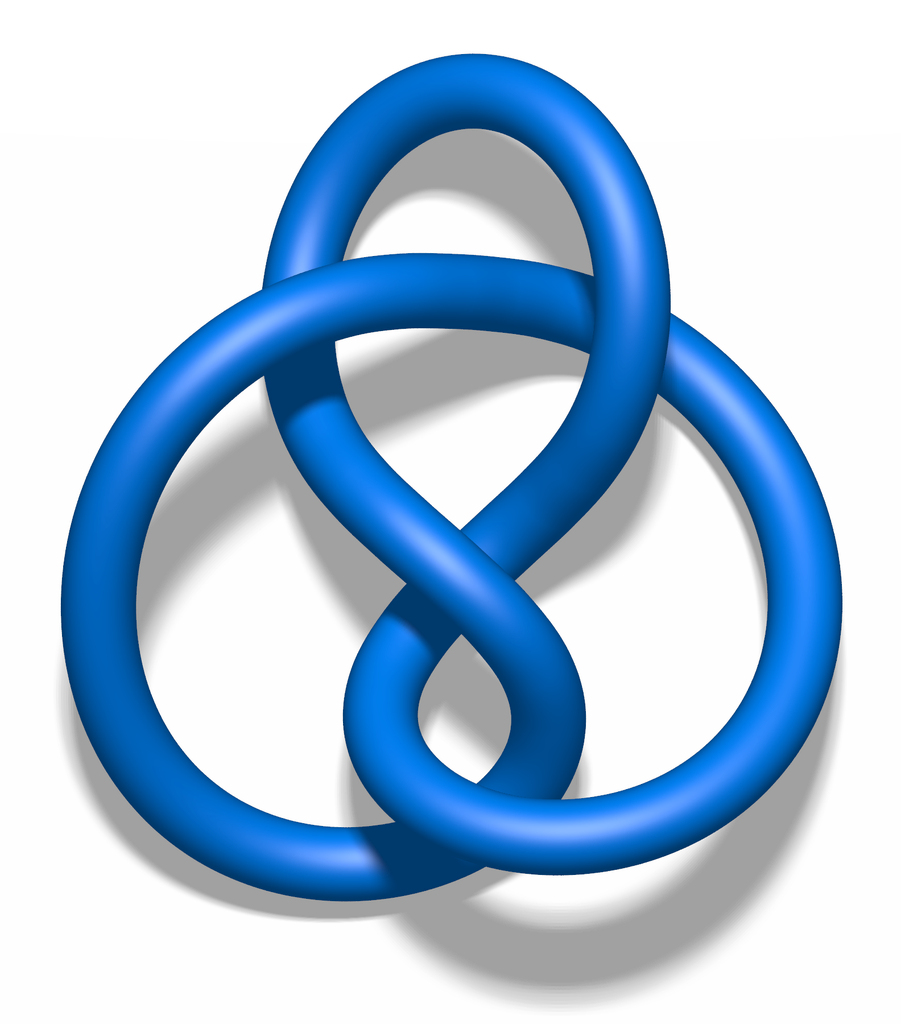
\includegraphics[width=0.2\linewidth, keepaspectratio]{figures/blue-eight-knot.png} 
            \label{fig:knot-eight-knot}
        }%
        \subfloat[$6_2$-Knoten]{
            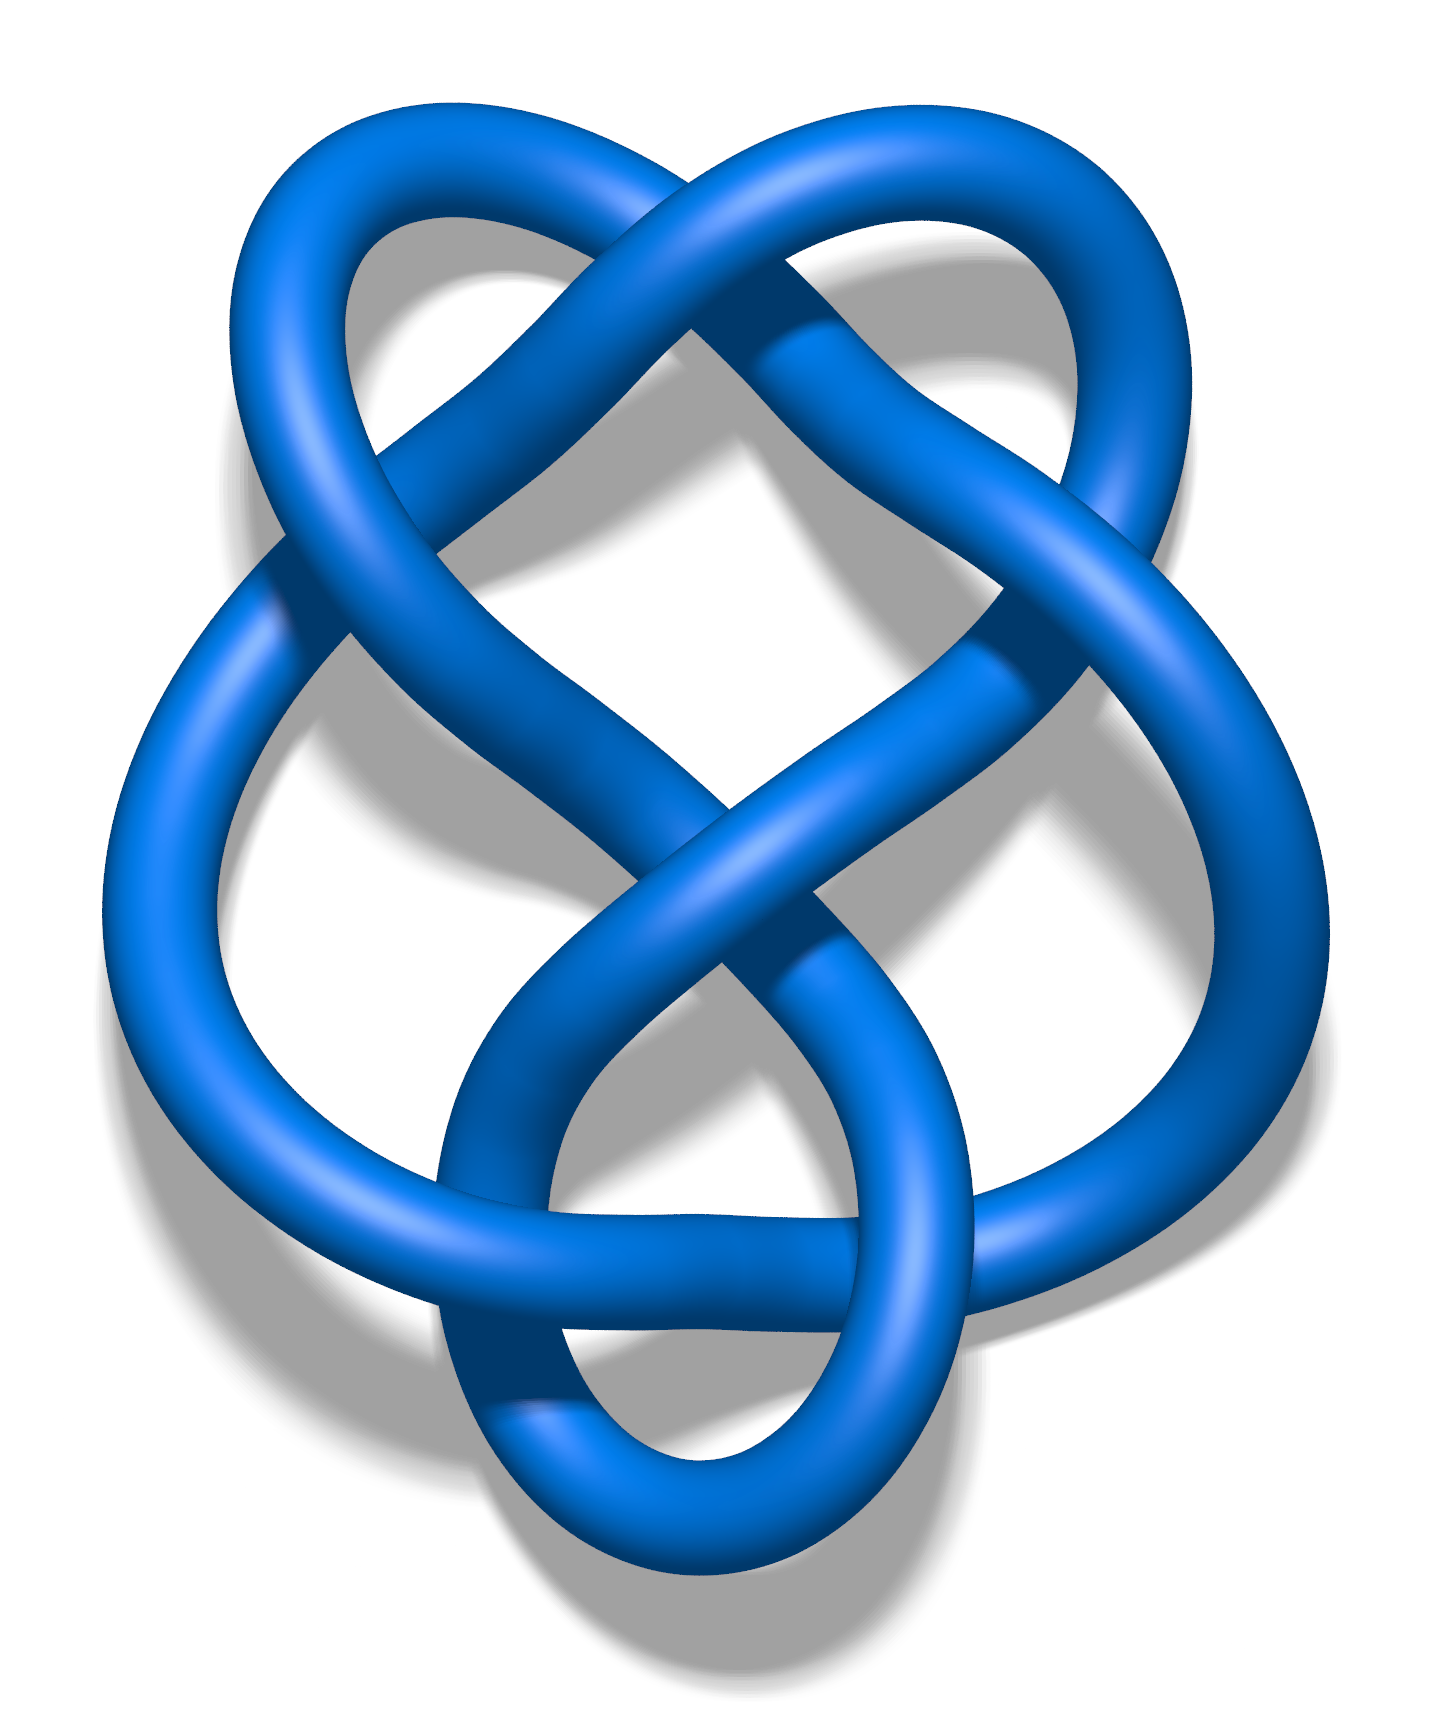
\includegraphics[width=0.2\linewidth, keepaspectratio]{figures/blue-6-2-knot.png} 
            \label{fig:knot-6-2}
        }

        \caption{Beispiele für verschiedene Knoten}
        \label{fig:Knoten}
    \end{figure}
\end{beispiel}

\begin{definition}\xindex{Knoten!äquivalente}\xindex{Isotopie}%
    Zwei Knoten $\gamma_1, \gamma_2: S^1 \rightarrow \mdr^3$ heißen
    \textbf{äquivalent}, wenn es eine stetige Abbildung
    $H: S^1 \times [0,1] \Rightarrow \mdr^3$ gibt mit 
    $H(z,0) = \gamma_1(z), H(z,1) = \gamma_2(z)$ und für jedes
    feste $t \in [0,1]$ ist $H_z: S^1 \rightarrow \mdr^2, z \mapsto H(z,t)$
    ein Knoten. Die Abbildung $H$ heißt \textbf{Isotopie} zwischen
    $\gamma_1$ und $\gamma_2$.
\end{definition}

\begin{definition}\xindex{Knotendiagramm}%
    Ein \textbf{Knotendiagramm} eines Knotens $\gamma$ ist eine 
    Projektion $\pi: \mdr^3 \rightarrow E$ auf eine Ebene $E$, sodass
    $|(\pi|C)^{-1}(x)| \leq 2$ für jedes $x \in D$.

    Ist $(\pi|C)^{-1}(x) = \Set{y_1, y_2}$, so \textbf{liegt $y_1$ über $y_2$},
    wenn $(y_1-x) = \lambda (y_2 - x)$ für ein $\lambda > 1$ ist.
\end{definition}

\begin{satz}[Satz von Reidemeister]
    Zwei endliche Knotendiagramme gehören genau dann zu äquivalenten
    Knoten, wenn sie durch endlich viele \enquote{Reidemeister-Züge}
    in einander überführt werden können.
\end{satz}

\begin{figure}[htp]
    \centering
    \subfloat[$\Omega_1$]{
        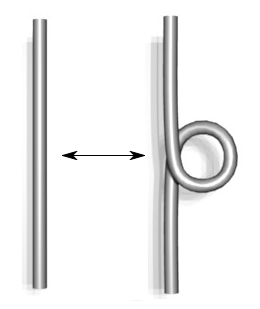
\includegraphics[height=0.2\linewidth, keepaspectratio]{figures/reidemeister-move-1.png} 
        \label{fig:reidemeister-1}
    }\qquad\qquad%
    \subfloat[$\Omega_2$]{
        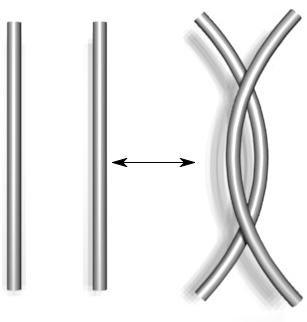
\includegraphics[height=0.2\linewidth, keepaspectratio]{figures/reidemeister-move-2.png} 
        \label{fig:reidemeister-2}
    }

    \subfloat[$\Omega_3$]{
        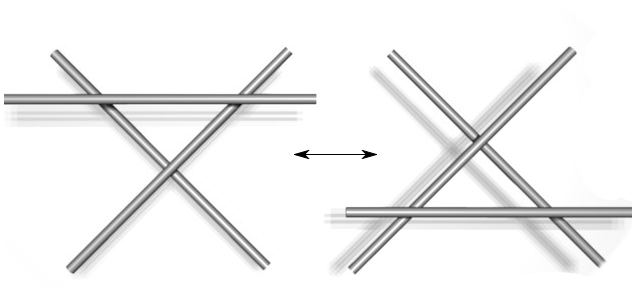
\includegraphics[height=0.2\linewidth, keepaspectratio]{figures/reidemeister-move-3.png} 
        \label{fig:reidemeister-3}
    }

    \caption{Reidemeister-Züge}
    \label{fig:reidemeister-zuege}
\end{figure}

\begin{beweis}
    Durch sorgfältige Fallunterscheidung.\footnote{Siehe \enquote{Knot Theory and Its Applications} von Kunio Murasugi. ISBN 978-0817638177.}
\end{beweis}

\begin{definition}\xindex{Färbbarkeit}%
    Ein Knotendiagramm heißt \textbf{3-färbbar}, 
    wenn jeder Bogen von $D$ so mit einer Farbe gefärbt werden kann, 
    dass an jeder Kreuzung eine oder 3 Farben auftreten und alle 3 
    Farben auftreten.
\end{definition}

\begin{figure}[htp]
    \centering
    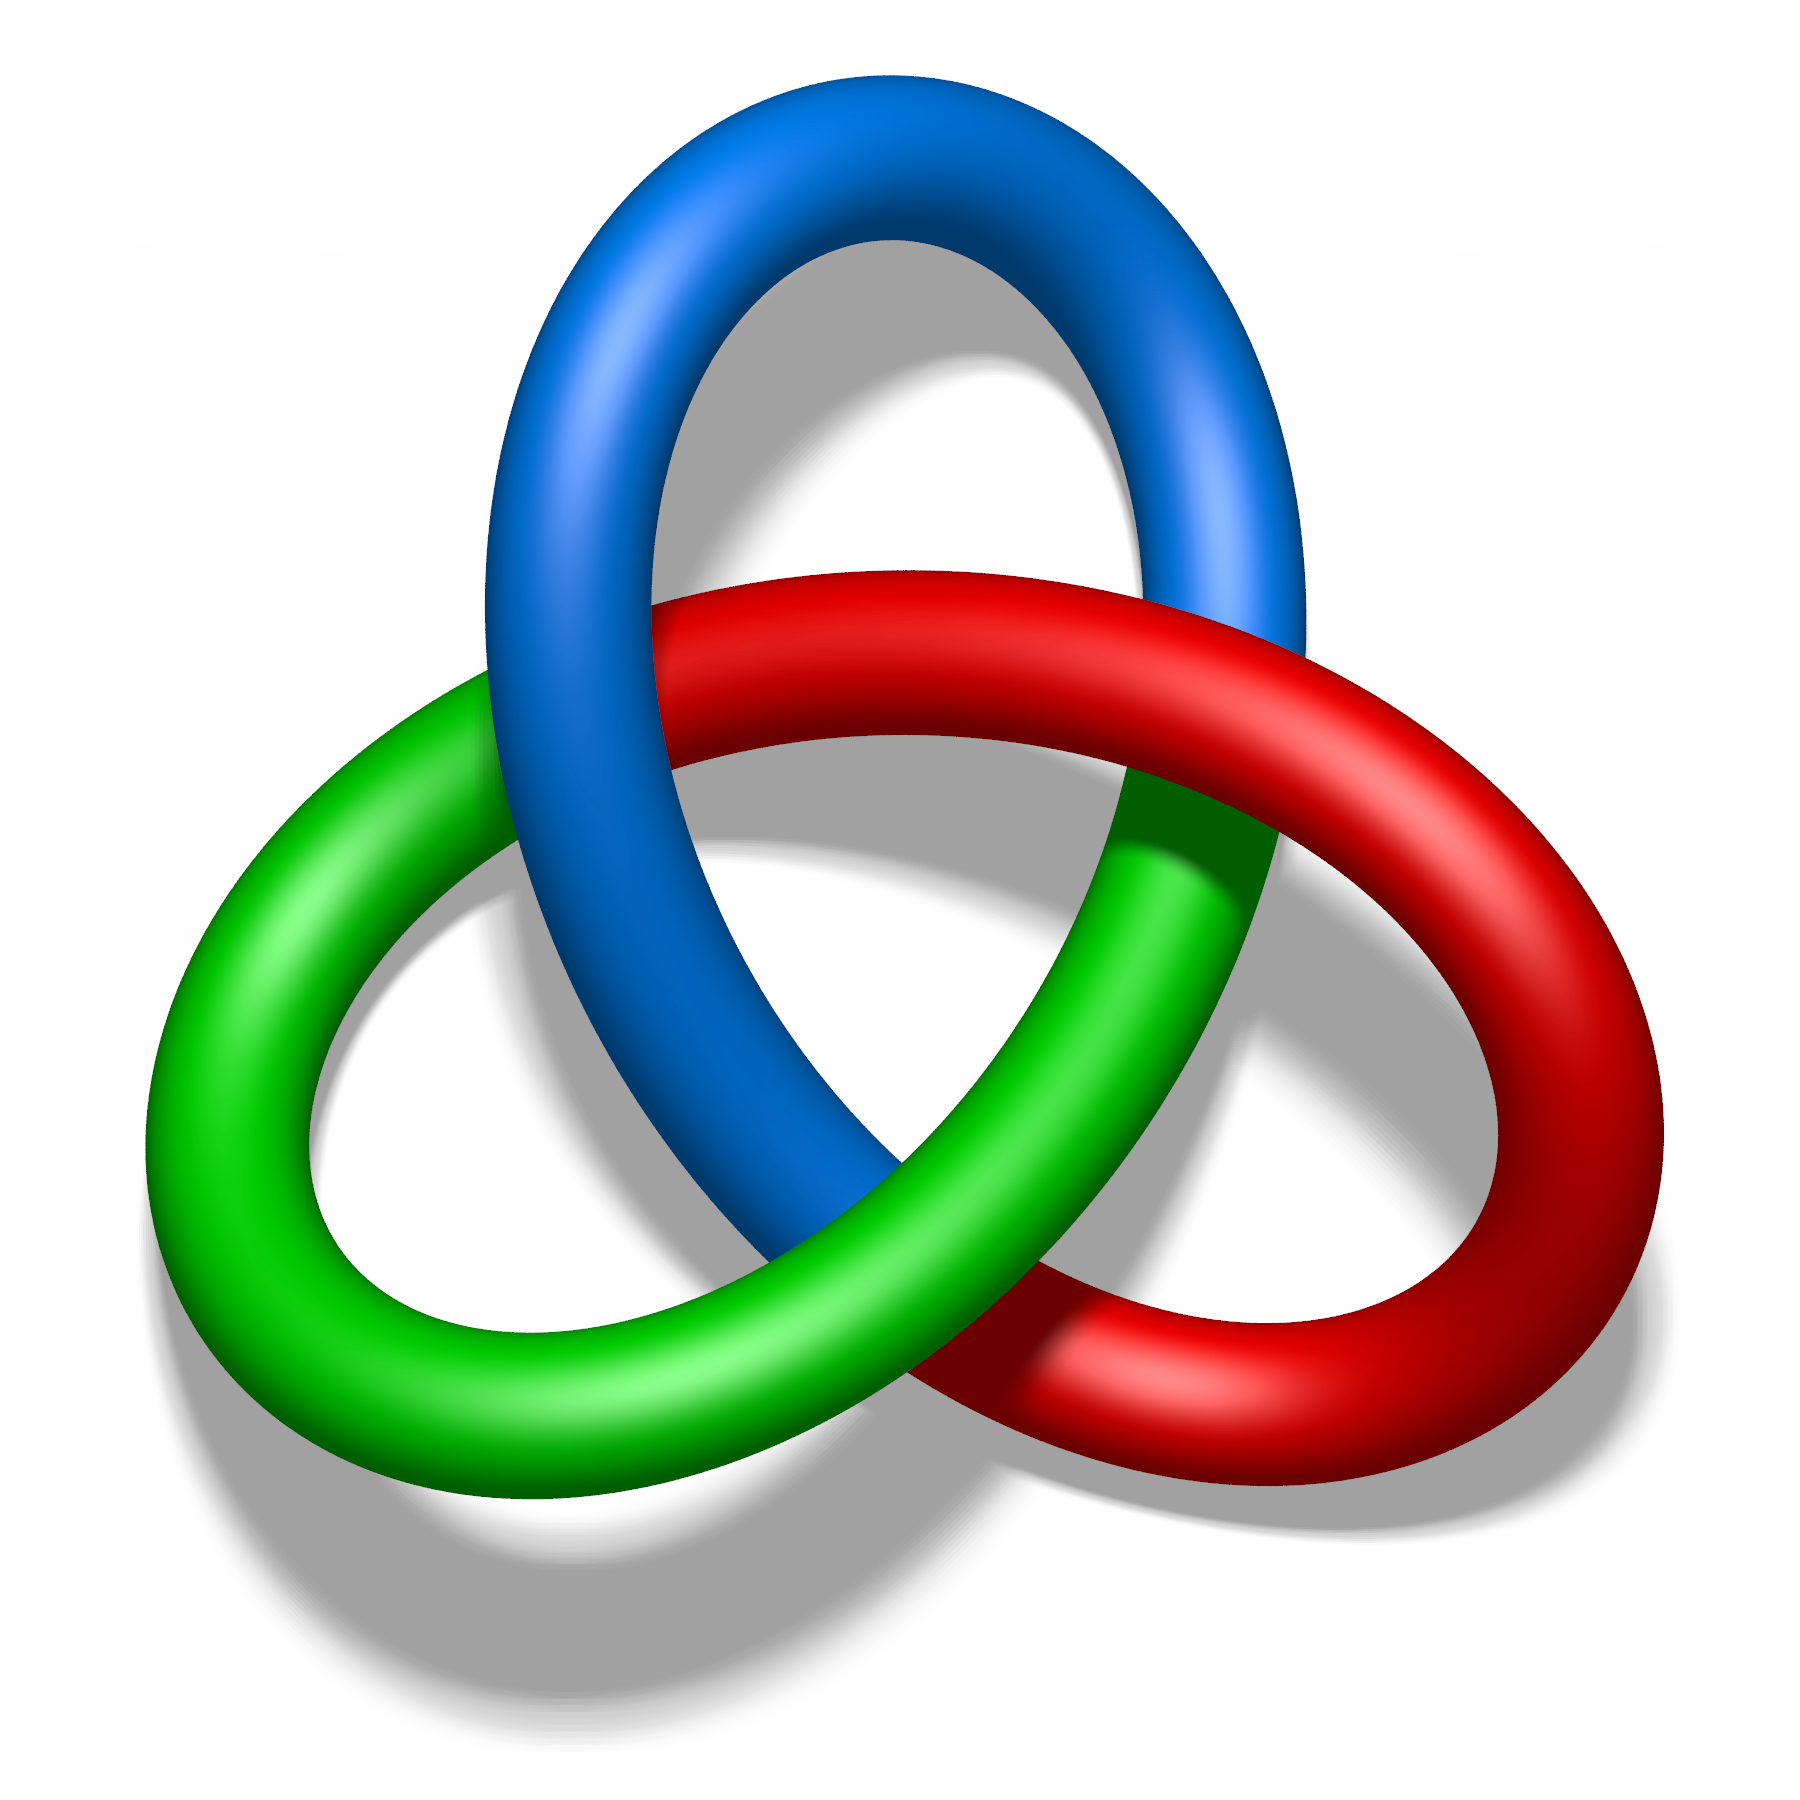
\includegraphics[height=0.3\linewidth, keepaspectratio]{figures/tricoloring.png} 

    \caption{Ein 3-gefärber Kleeblattknoten}
    \label{fig:treefoil-knot-three-colors}
\end{figure}
\index{Knoten|)}

% Die Übungsaufgaben sollen ganz am Ende des Kapitels sein.
\clearpage
\section*{Übungsaufgaben}
\addcontentsline{toc}{section}{Übungsaufgaben}

\begin{aufgabe}[Sierpińskiraum]\label{ub:aufg1}
    Es sei $X := \Set{0,1}$ und $\fT_X := \Set{\emptyset, \Set{0}, X}$.
    Dies ist der sogenannte Sierpińskiraum.
    \begin{enumerate}[label=(\alph*)]
        \item Beweisen Sie, dass $(X, \fT_X)$ ein topologischer Raum ist.
        \item Ist $(X, \fT_X)$ hausdorffsch?
        \item Ist $\fT_X$ von einer Metrik erzeugt?
    \end{enumerate}
\end{aufgabe}

\begin{aufgabe}\label{ub:aufg4}
    Es sei $\mdz$ mit der von den Mengen $U_{a,b} := a + b \mdz (a \in \mdz, b \in \mdz \setminus \Set{0})$
    erzeugten Topologie versehen.

    Zeigen Sie:
    \begin{enumerate}[label=(\alph*)]
        \item Jedes $U_{a,b}$ und jede einelementige Teilmenge von $\mdz$ ist abgeschlossen.
        \item Die $U_{a,b}$ bilden eine Basis der Topologie.
        \item $\Set{-1, 1}$ ist nicht offen.
        \item Es gibt unendlich viele Primzahlen.
    \end{enumerate}
\end{aufgabe}


%%%%%%%%%%%%%%%%%%%%%%%%%%%%%%%%%%%%%%%%%%%%%%%%%%%%%%%%%%%%%%%%%%%%%
% Henriekes Mitschrieb vom 07.11.2013                               %
%%%%%%%%%%%%%%%%%%%%%%%%%%%%%%%%%%%%%%%%%%%%%%%%%%%%%%%%%%%%%%%%%%%%%
\chapter{Mannigfaltigkeiten und Simplizialkomplexe}
\section{Topologische Mannigfaltigkeiten}
\begin{definition}%
    Sei $X$ ein topologischer Raum und $n \in \mdn$.
    \begin{defenum}
        \item Eine $n$-dimensionale \textbf{Karte}\xindex{Karte} auf
              $X$ ist ein Paar $(U, \varphi)$, wobei $U \subseteq X$
              offen und $\varphi: U \rightarrow V$ Homöomorphismus
              von $U$ auf eine offene Teilmenge $V \subseteq \mdr^n$.
        \item Ein $n$-dimensionaler \textbf{Atlas}\xindex{Atlas} $\atlas$ auf $X$ ist eine
              Familie $(U_i, \varphi_i)_{i \in I}$ von Karten auf $X$,
              sodass $\bigcup_{i \in I} U_i = X$.
        \item $X$ heißt (topologische) $n$-dimensionale \textbf{Mannigfaltigkeit}\xindex{Mannigfaltigkeit},
              wenn $X$ hausdorffsch ist, eine abzählbare Basis der 
              Topologie hat und ein $n$-dimensionalen Atlas besitzt.
    \end{defenum}
\end{definition}

\begin{bemerkung}
    \begin{bemenum}
        \item Es gibt surjektive, stetige Abbildungen $[0,1] \rightarrow [0,1] \times [0,1]$
        \item Für $n \neq m$ sind $\mdr^n$ und $\mdr^m$ nicht homöomorph.
              Zum Beweis benutzt man den \enquote{Satz von der Gebietstreue} (Brouwer):

              Ist $U \subseteq \mdr^n$ offen und $f: U \rightarrow \mdr^n$
              stetig und injektiv, so ist $f(U)$ offen.

              Ist $n < m$ und $\mdr^m$ homöomorph zu $\mdr^n$, so wäre
              \[f:\mdr^n \rightarrow \mdr^m \rightarrow \mdr^n, \;\;\; (x_1, \dots, x_n) \mapsto (x_1, x_2, \dots, x_n, 0, \dots, 0)\]
              eine stetige injektive Abbildung. Also müsste $f(\mdr^n)$
              offen sein $\Rightarrow$ Widerspruch
    \end{bemenum}
\end{bemerkung}

\begin{beispiel}[Mannigfaltigkeiten]
    \begin{bspenum}
        \item Jede offene Teilmenge $U \subseteq \mdr^n$ ist eine 
              $n$-dimensionale Mannigfaltigkeit mit einem Atlas aus 
              einer Karte.
        \item $\mdc^n$ ist eine $2n$-dimensionale Mannigfaltigkeit
              mit einem Atlas aus einer Karte:
              \[(z_1, \dots, z_n) \mapsto (\Re(z_1), \Im(z_1), \dots, \Re(z_n), \Im(z_n))\]
        \item \xindex{Raum!projektiver}$\praum^n(\mdr) = (\mdr^{n+1} \setminus \Set{0})/_\sim = S^n /_\sim$ und $\praum^n(\mdc)$ sind Mannigfaltigkeiten
              der Dimension $n$ bzw. $2n$, da gilt:

              Sei $U_i := \Set{(x_0: \dots : x_n) \in \praum^n(\mdr) | x_i \neq 0}\;\forall i \in 0, \dots, n$.
              Dann ist $\praum^n(\mdr) = \bigcup_{i=0}^n U_i$ und die Abbildung
              \begin{align*}
                U_i &\rightarrow \mdr^n\\
                (x_0 : \dots : x_n) &\mapsto \left (\frac{x_0}{x_i}, \dots, \frac{x_i}{x_i}, \dots, \frac{x_n}{x_i} \right )\\
                (y_1 : \dots : y_{i-1} : 1 : y_i : \dots : y_n) &\mapsfrom (y_1, \dots, y_n)
              \end{align*}
              ist bijektiv.
              \todo[inline]{Was wird im Folgenden gemacht?}
              Die $U_i$ mit $i = 0, \dots, n$ bilden einen $n$-dimensionalen Atlas:
              \begin{align*}
                      x &= (1:0:0) \in U_0 \rightarrow \mdr^2 & x &\mapsto (0,0)\\
                      y &= (0:1:1) \in U_2 \rightarrow \mdr^2 & y &\mapsto (0,1)
              \end{align*}
              $\text{Umgebung: } \fB_1 (0,1) \rightarrow \Set{(1:u:v) | \|(u,v)\| < 1} = V_1$\\
              $\text{Umgebung: } \fB_1 (0,1) \rightarrow \Set{(w:z:1) | w^2 + z^2 < 1} = V_2$\\

              $V_1 \cap V_2 = \emptyset$?

              $(a:b:c) \in V_1 \cap V_2$\\
              $\Rightarrow a \neq 0$ und $(\frac{b}{a})^2 + (\frac{c}{a})^2 < 1 \Rightarrow \frac{c}{a} < 1$\\
              $\Rightarrow c \neq 0$ und $(\frac{a}{c})^2 + (\frac{b}{c})^2 < 1 \Rightarrow \frac{a}{c} < 1$\\
              $\Rightarrow$ Widerspruch
        \item $S^n = \Set{x \in \mdr^{n+1} | \|x\| = 1}$ ist $n$-dimensionale
              Mannigfaltigkeit.

              Karten: \\
              $O_i := \Set{(x_1, \dots, x_{n+1}) \in S^n | x_i > 0} \rightarrow \fB_1 (\underbrace{0, \dots, 0}_{\in \mdr^n})$\\
              $(x_1, \dots, x_{n+1}) \mapsto (x_1, \dots, x_i, \dots, x_{n+1})$\\
              $(x_1, \dots, x_{i-1}, \sqrt{1-\sum_{k=1}^n x_k^2}, x_i, \cdots, x_n)\mapsfrom (x_1, \dots, x_n)$\\
              $S^n = \bigcup_{i=1}^{n+1} (C_i \cup D_i)$
        \item $[0,1]$ ist keine Mannigfaltigkeit, denn:\\
              Es gibt keine Umgebung von $0$ in $[0,1]$, die homöomorph
              zu einem offenem Intervall ist.
        \item $V_1 = \Set{(x,y) \in \mdr^2 | x \cdot y = 0}$ ist
              keine Mannigfaltigkeit. 

              Das Problem ist $(0,0)$. Wenn man diesen Punkt entfernt,
              zerfällt der Raum in 4 Zusammenhangskomponenten.
              Jeder $\mdr^n$ zerfällt jedoch in höchstens zwei
              Zusammenhangskomponenten, wenn man einen Punkt entfernt.
        \item $V_2 = \Set{(x,y) \in \mdr^2 | x^3 = y^2}$ ist eine
              Mannigfaltigkeit.
        \item $X = (\mdr \setminus \Set{0}) \cup (0_1, 0_2)$ \label{bsp:mannigfaltigkeit8}

              \[U \subseteq X \text{ offen } \gdw 
                \begin{cases}
                    U \text{ offen in } \mdr \setminus \Set{0}, &\text{falls } 0_1 \notin U, 0_2 \in U\\
                    \exists \varepsilon > 0: (-\varepsilon, \varepsilon) \subseteq U &\text{falls } 0_1 \in U, 0_2 \in U
                \end{cases}\]
              Insbesondere sind $(\mdr \setminus \Set{0}) \cup \Set{0_1}$
              und $(\mdr \setminus \Set{0}) \cup \Set{0_2}$ offen und
              homöomorph zu $\mdr$.

              \underline{Aber:} $X$ ist nicht hausdorffsch!
              Denn es gibt keine disjunkten Umgebungen von $0_1$ und
              $0_2$.
        \item \xindex{Gruppe!allgemeine lineare}$\GL_n(\mdr)$ ist eine Mannigfaltigkeit der Dimension 
              $n^2$, weil offene Teilmengen von $\mdr^{n^2}$ eine
              Mannigfaltigkeit bilden.
    \end{bspenum}
\end{beispiel}

%%%%%%%%%%%%%%%%%%%%%%%%%%%%%%%%%%%%%%%%%%%%%%%%%%%%%%%%%%%%%%%%%%%%%
% Mitschrieb vom 14.11.2013                                         %
%%%%%%%%%%%%%%%%%%%%%%%%%%%%%%%%%%%%%%%%%%%%%%%%%%%%%%%%%%%%%%%%%%%%%
\begin{definition}\xindex{Verklebung}%
    Seien $X, Y$ $n$-dimensionale Mannigfaltigkeiten, $U \subseteq X$
    und $V \subseteq Y$ offen, $\Phi: U \rightarrow V$ ein Homöomorphismus
    $Z = (X \dcup Y) /_\sim$ mit der von $u \sim \Phi(u)\;\forall{u \in U}$
    erzeugten Äquivalenzrelation und der von $\sim$ induzierten 
    Quotiententopologie.

    $Z$ heißt \textbf{Verklebung} von $X$ und $Y$ längs $U$ und $V$.
    $Z$ besitzt einen Atlas aus $n$-dimensionalen Karten.
    Falls $Z$ hausdorffsch ist, ist $Z$ eine $n$-dimensionale 
    Mannigfaltigkeit.
\end{definition}

\begin{bemerkung}
    Sind $X, Y$ Mannigfaltigkeiten der Dimension $n$ bzw. $m$, so ist
    $X \times Y$ eine Mannigfaltigkeit der Dimension $n+m$.
\end{bemerkung}

\begin{beweis}
    Produkte von Karten sind Karten. $\qed$
\end{beweis}

\begin{beispiel}
    Mannigfaltigkeiten mit Dimension 1:
    \begin{enumerate}[label=\arabic*)]
        \item Offene Intervalle, $\mdr$, $(0,1)$ sind alle homöomorph
        \item $S^1$
    \end{enumerate}

    Mannigfaltigkeiten mit Dimension 2:
    \begin{enumerate}[label=\arabic*)]
        \item $\mdr^2$
        \item $S^2$ (0 Henkel)
        \item $T^2$ (1 Henkel)
        \item oder mehr Henkel, wie z.B. der Zweifachtorus in \cref{fig:double-torus}
    \end{enumerate}

    \begin{figure}[htp]
        \centering
        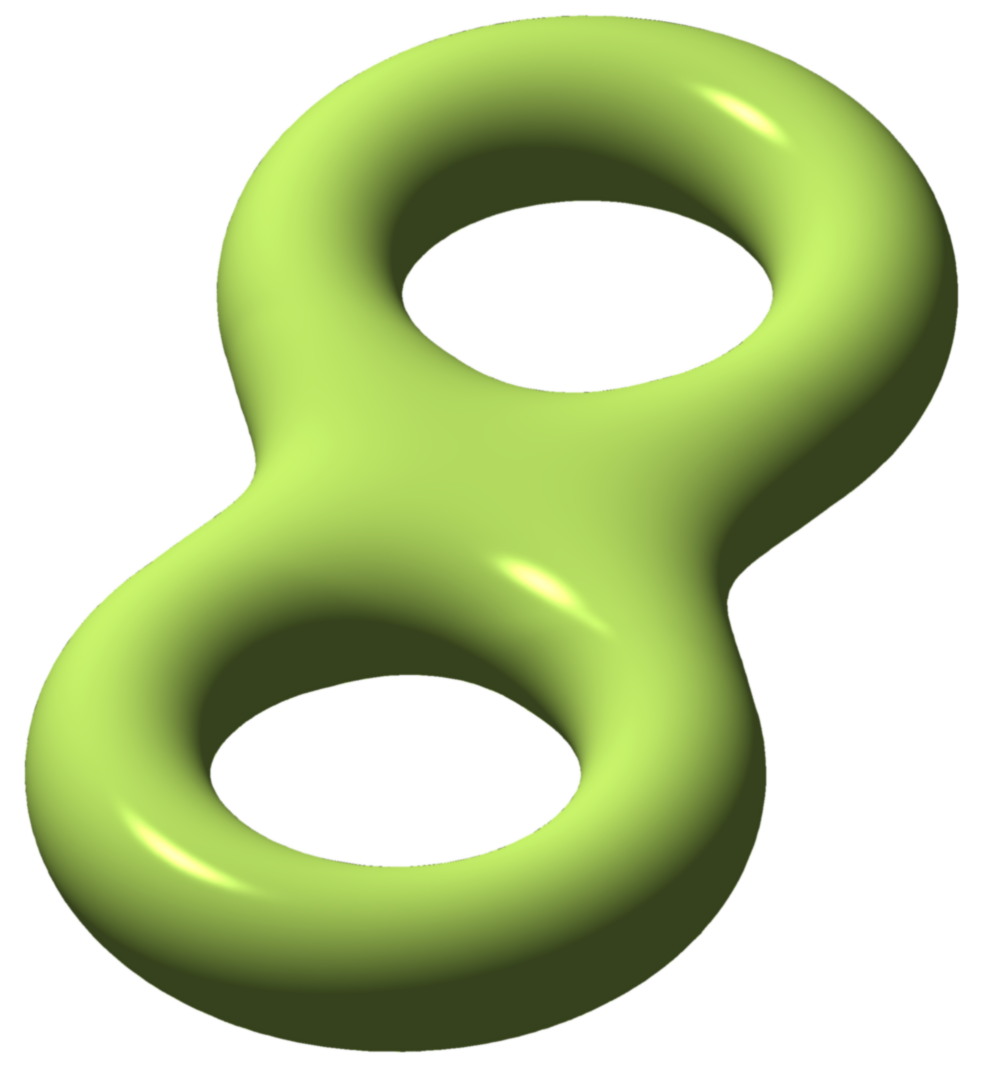
\includegraphics[width=0.2\linewidth, keepaspectratio]{figures/Double-torus-illustration.png}
        \caption{Zweifachtorus}
        \label{fig:double-torus}
    \end{figure}
\end{beispiel}

\begin{bemerkung}
    Sei $n \in \mdn, F:\mdr^n \rightarrow \mdr$ stetig differenzierbar
    und $X = V(F) := \Set{x \in \mdr^n | F(x) = 0}$ das \enquote{vanishing set}\xindex{vanishing set}.

    Dann gilt:
    \begin{bemenum}
        \item $X$ ist abgeschlossen in $\mdr^n$
        \item Ist $\grad(F)(X) \neq 0 \;\;\;\forall{x \in X}$, so ist
              $X$ eine Mannigfaltigkeit der Dimension $n-1$.  \label{bem:Mannigfaltigkeitskriterium}
    \end{bemenum}
\end{bemerkung}

\begin{beweis}\leavevmode
    \begin{enumerate}[label=\alph*),ref=\thedefinition.\alph*]
        \item Sei $y \in \mdr^n \setminus V(F)$. Weil $F$ stetig ist,
              gibt es $\delta > 0$, sodass $F(\fB_\delta(y)) \subseteq \fB_\varepsilon(F(y))$
              mit $\varepsilon = \frac{1}{2} \|F(y)\|$. Folgt
              $\fB_\delta(y) \cap V(F) = \emptyset \Rightarrow \mdr^n \setminus V(F)$
              ist offen.
        \item Sei $x \in X$ mit $\grad(F)(x) \neq 0$, also
              \obda $\frac{\partial F}{\partial X_1} (x) \neq 0$,
              $x = (x_1, \dots, x_n)$, $x' := (x_2, \dots, x_n) \in \mdr^{n-1}$.
              Der Satz von der impliziten Funktion liefert nun:
              Es gibt Umgebungen $U$ von $x'$ und differenzierbare
              Funktionen $g: U \rightarrow \mdr$, sodass
              $G: U \rightarrow \mdr^n, \; u \mapsto (g(u), u)$
              eine stetige Abbildung auf eine offene Umgebung $V$ von
              $x$ in $X$ ist.
    \end{enumerate}  
    $\qed$
\end{beweis}

\begin{beispiel}\xindex{Neilsche Parabel}%
    \begin{bspenum}
        \item $F: \mdr^3 \rightarrow \mdr,\;\;\; (x, y, z) \mapsto x^2 + y^2 + z^2 - 1$,
              $V(F) = S^2$, $\grad(F) = (2x, 2y, 2z) \xRightarrow{\crefabbr{bem:Mannigfaltigkeitskriterium}} S^n$
              ist $n$-dimensionale Mannigfaltigkeit in $\mdr^{n+1}$
        \item $F: \mdr^2 \rightarrow \mdr, \;\;\; (x,y) \mapsto y^2 - x^3$
            \begin{figure}[ht]
                \centering
                \subfloat[$F(x,y) = y^2 - x^3$]{
                    \resizebox{0.45\linewidth}{!}{\documentclass{article}
\usepackage[pdftex,active,tightpage]{preview}
\setlength\PreviewBorder{2mm}
\usepackage{pgfplots}
\pgfplotsset{compat=1.9}

\begin{document}
\begin{preview}
\pgfplotsset{
    colormap={whitered}{
        color(0cm)=(white);
        color(1cm)=(orange!75!red)
    }
}
\begin{tikzpicture}[scale=0.5]
    \begin{axis}[
    colormap name=whitered,
    width=6cm,
    view={155}{45},
    enlargelimits=false,
    grid=major,
    domain=-5:5,
    y domain=-5:5,
    samples=56, %57 : TeX capacity exceeded, sorry [main memory size=3000000].
                % see also http://tex.stackexchange.com/a/7954/5645
    xlabel=$x$,
    ylabel=$y$,
    zlabel={$z$},
    colorbar,
    colorbar style={
        at={(-0.1,0)},
        anchor=south west,
        height=0.25*\pgfkeysvalueof{/pgfplots/parent axis height},
        title={$f(x,y)$}
    }
    ]
      \addplot3[surf] {y*y-x*x*x};
    \end{axis} 
\end{tikzpicture}
\end{preview}
\end{document}
}
                    \label{fig:semicubical-parabola-2d}
                }%
                \subfloat[$y^2 - ax^3 = 0$]{
                    \resizebox{0.45\linewidth}{!}{\documentclass[varwidth=true, border=2pt]{standalone}

\usepackage{pgfplots}
\usepackage{tikz}

\begin{document}
\begin{tikzpicture}
    \begin{axis}[
        legend pos=south east,
        axis x line=middle,
        axis y line=middle,
        grid = major,
        %width=9cm,
        %height=4.5cm,
        grid style={dashed, gray!30},
        xmin= 0,     % start the diagram at this x-coordinate
        xmax= 12,    % end   the diagram at this x-coordinate
        ymin=-10,     % start the diagram at this y-coordinate
        ymax= 10,   % end   the diagram at this y-coordinate
        %axis background/.style={fill=white},
        xlabel=$x$,
        ylabel=$y$,
        %xticklabels={-2,-1.6,...,7},
        tick align=outside,
        %minor tick num=-3,
        enlargelimits=true]
      \addplot[domain=0:12, red, thick,samples=500] {1/3*x^1.5}; 
      \addplot[domain=0:12, orange, thick,samples=500] {1*x^1.5}; 
      \addplot[domain=0:12, blue, thick,samples=500] {2*x^1.5}; 

      \addplot[domain=0:12, red, thick,samples=500] {-1/3*x^1.5}; 
      \addplot[domain=0:12, orange, thick,samples=500] {-1*x^1.5}; 
      \addplot[domain=0:12, blue, thick,samples=500] {-2*x^1.5}; 
      \addlegendentry{$a=\frac{1}{3}$}
      \addlegendentry{$a=1$}
      \addlegendentry{$a=2$}
    \end{axis} 
\end{tikzpicture}
\end{document}
}
                    \label{fig:semicubical-parabola-3d}
                }%
                \label{Neilsche-Parabel}
                \caption{Rechts ist die Neilsche Parabel für verschiedene Parameter $a$.}
            \end{figure}
              Es gilt: $\grad(F) = (-3x^2, 2y)$. Also: $\grad(0,0) = (0,0)$.
              Daher ist \cref{bem:Mannigfaltigkeitskriterium}
              nicht anwendbar, aber $V(F)$ ist trotzdem
              eine 1-dimensionale topologische Mannigfaltigkeit.
    \end{bspenum}
\end{beispiel}

\begin{definition}\xindex{Mannigfaltigkeit!mit Rand}%
    Sei $X$ ein Hausdorffraum mit abzählbarer Basis der Topologie.
    $X$ heißt $n$-dimensionale \textbf{Mannigfaltigkeit mit Rand},
    wenn es einen Atlas $(U_i, \varphi_i)$ gibt, wobei $U_i \subseteq X_i$
    offen und $\varphi_i$ ein Homöomorphismus auf eine offene 
    Teilmenge von 
    \[R_{+,0}^n := \Set{(x_1, \dots, x_n) \in \mdr^n | x_m \geq 0}\]
    ist. $R_{+,0}^n$ ist ein \enquote{Halbraum}.
\end{definition}

\begin{figure}[ht]
    \centering
    \subfloat[Halbraum]{
        \begin{tikzpicture}
    \draw [white,step=0.5cm, pattern=north east lines] (0,0) rectangle (2,1);
    \draw[very thick] (0,0) -- (2,0);

    \node at (2.4,0.5) {$\stackrel{\sim}{=}$};

\begin{scope}[shift={(4,0)}]
    \draw[white,pattern=north east lines] ([shift={(180:1cm)}]-0.0,0) arc (180:0:1cm);
    \draw[very thick] (-1,0) -- (1,0);
\end{scope}
\end{tikzpicture}

        \label{fig:half-space}
    }%

    \subfloat[Pair of pants]{
        \resizebox{0.45\linewidth}{!}{\begin{tikzpicture}[tqft/flow=east]
    \node[tqft/pair of pants,draw,rotate=-180] (a) {};
    \draw (-1.02,-1) ellipse (0.2cm and 0.35cm);
    \draw (-1.02,+1) ellipse (0.2cm and 0.35cm);
    \draw[dashed] (1,0) ellipse (0.175cm and 0.35cm);

    \draw (2.3,0) ellipse (0.7cm and 1.5cm);
    \draw (2.3,+0.5) circle (0.3cm);
    \draw (2.3,-0.5) circle (0.3cm);

    \node at (1.38,0) {$\stackrel{\sim}{=}$};
\end{tikzpicture}
}
        \label{fig:pair-of-pants}
    }%
    \subfloat[Sphäre mit einem Loch]{
        \resizebox{0.45\linewidth}{!}{\begin{tikzpicture}[tqft/flow=east]
    \draw (0,0) circle (2cm);
    \draw (0,0) ellipse (2cm and 0.35cm);
    \draw[white,fill=white] (0,0.1) ellipse (1.95cm and 0.35cm);
    \draw[dashed] (0,0) ellipse (2cm and 0.35cm);

    \begin{scope}[rotate=45]
        \draw (0.5,1.2) ellipse (0.5cm and 0.4cm);
    \end{scope}

    \node at (2.38,0) {$\stackrel{\sim}{=}$};

    \draw (3.8,0) circle (1cm);
\end{tikzpicture}
}
        \label{fig:sphere-with-hole}
    }%
    \label{Mannigfaltigkeiten mit Rand}
    \caption{Beispiele für Mannigfaltigkeiten mit Rand}
\end{figure}

\begin{definition}\xindex{Rand}%
    Sei $X$ eine $n$-dimensionale Mannigfaltigkeit mit Rand und
    Atlas $(U_i, \varphi_i)$. Dann heißt 
    \[\partial X := \bigcup_{i\in I} \Set{x \in U_i | \varphi_i (x)_n = 0}\]
    \textbf{Rand} von $X$.
\end{definition}

$\partial X$ ist eine Mannigfaltigkeit der Dimension $n-1$.

\begin{definition}\xindex{Kartenwechsel}\index{Uebergangsfunktion@""Ubergangsfunktion|see{Kartenwechsel}}%
    Sei $X$ eine $n$-dimensionale Mannigfaltigkeit mit Atlas
    $(U_i, \varphi_i)_{i \in I}$

    Für $i, j \in I$ mit $U_i, U_j \neq \emptyset$ heißt
              \begin{align*}
                \varphi_{ij} &:= \varphi_j \circ \varphi_i^{-1}\\
                \varphi_i (U_i \cap U_j) &\rightarrow \varphi_j (U_i \cap U_j)
              \end{align*}
              \textbf{Kartenwechsel} oder \textbf{Übergangsfunktion}.
\end{definition}

\begin{figure}[htp]
    \centering
    \documentclass[varwidth=true, border=2pt]{standalone}
\usepackage{amsmath,amssymb}% math symbols / fonts
\usepackage{tikz}
\usepackage{tqft}
\usetikzlibrary{patterns}

\begin{document}
    \begin{tikzpicture}[tqft/flow=east]
        \draw (0,0) ellipse (2cm and 1cm);
        \draw (0,-2) ellipse (3cm and 0.8cm);
        \def\ringa{(-0.3,0) circle (0.5cm)}
        \def\ringb{(+0.3,0) circle (0.5cm)}

        \begin{scope}[even odd rule]
            \clip \ringa;
            \fill[pattern color=red,pattern=north east lines] \ringb;
        \end{scope}

        \begin{scope}[even odd rule,shift={(-0.7,-2)}]
            \clip \ringa;
            \fill[draw=red,pattern color=red,pattern=north east lines] \ringb;
        \end{scope}

        \begin{scope}[even odd rule,shift={(+0.7,-2)}]
            \clip \ringb;
            \fill[draw=red,pattern color=red,pattern=north east lines] \ringa;
        \end{scope}
        \draw \ringa;
        \draw \ringb;

        \node at (-1,0.3) {$U_i$};
        \node at (+1,0.3) {$U_j$};
        \node at (-1.9,-2) {$V_i$};
        \node at (+1.9,-2) {$V_j$};
        \node at (+2.0,0.7) {$X$};
        \node at (+2.4,-1.3) {$\mathbb{R}^n$};


        \path[->] (-0.35,0)  edge [bend angle=10,bend right] node[label={[label distance=0.1cm]210:$\varphi_i$}] {} (-1,-1.5);
        \path[->] (+0.35,0)  edge [bend angle=10,bend left]  node[label={[label distance=0.1cm]-30:$\varphi_j$}] {} (+1,-1.5);

        \draw (-1,-2) circle (0.5cm);
        \draw (+1,-2) circle (0.5cm);

        \draw[->, red, thick] (-0.3,-2) -- (0.3,-2);
    \end{tikzpicture}
\end{document}

    \caption{Kartenwechsel}
    \label{fig:kartenwechsel}
\end{figure}

%%%%%%%%%%%%%%%%%%%%%%%%%%%%%%%%%%%%%%%%%%%%%%%%%%%%%%%%%%%%%%%%%%%%%
% Mitschrieb vom 19.11.2013                                         %
%%%%%%%%%%%%%%%%%%%%%%%%%%%%%%%%%%%%%%%%%%%%%%%%%%%%%%%%%%%%%%%%%%%%%
\section{Differenzierbare Mannigfaltigkeiten}\label{sec:8}
\begin{definition}%
    Sei $X$ eine $n$-dimensionale Mannigfaltigkeit mit Atlas $(U_i, \varphi_i)_{i \in I}$.

    \begin{defenum}
        \item $X$ heißt \textbf{differenzierbare Mannigfaltigkeit der Klasse $C^k$}\xindex{Mannigfaltigkeit!differenzierbare},
              wenn jede Kartenwechselabbildung $\varphi_{ij},\;i,j \in I$
              $k$-mal stetig differenzierbar ist.
        \item $X$ heißt \textbf{differenzierbare Mannigfaltigkeit}\xindex{Mannigfaltigkeit!glatte},
              wenn $X$ eine differenzierbare Mannigfaltigkeit der
              Klasse $C^\infty$ ist.
    \end{defenum}
\end{definition}

Differenzierbare Mannigfaltigkeiten der Klasse $C^\infty$ werden auch
\textit{glatt} genannt.

\begin{definition}%
    Sei $X$ eine differenzierbare Mannigfaltigkeit der Klasse $C^k$ 
    ($k \in \mdn \cup \Set{\infty}$) mit Atlas $(U_i, \varphi_i)_{i \in I}$.

    \begin{defenum}
        \item Eine Karte $(U, \varphi)$ auf $X$ heißt \textbf{verträglich}\xindex{verträglich}
              mit $\atlas$, wenn alle Kartenwechsel $\varphi \circ \varphi_i^{-1}$
              und $\varphi_i \circ \varphi^{-1}$ ($i \in I$ mit $U_i \cap U \neq \emptyset$)
              differenzierbar von Klasse $C^k$ sind.
        \item Die Menge aller mit $\atlas$ verträglichen Karten auf 
              $X$ bildet einen maximalen Atlas der Klasse $C^k$. Er
              heißt \textbf{$C^k$-Struktur}\xindex{Ck-Struktur@$C^k$-Struktur} auf $X$.
            
              Eine $C^\infty$-Struktur heißt auch \textbf{differenzierbare Struktur}\xindex{Struktur!differenzierbare}
              auf $X$.
    \end{defenum}
\end{definition}

\begin{bemerkung}
    Für $n \geq 4$ gibt es auf $S^n$ mehrere verschiedene differenzierbare
    Strukturen, die sog. \enquote{exotische Sphären}\xindex{Sphäre!exotische}.
\end{bemerkung}

\begin{definition}
    Seien $X, Y$ differenzierbare Mannigfaltigkeiten der Dimension
    $n$ bzw. $m$, $x \in X$.

    \begin{defenum}
        \item Eine stetige Abbildung $f:X \rightarrow Y$ heißt\label{def:stetigeAbbildungDiffbar}
              \textbf{differenzierbar}\xindex{Abbildung!differenzierbare}
              in $x$ (von Klasse $C^k$),
              wenn es Karten $(U, \varphi)$ von $X$ mit
              $x \in U$ und $(V, \psi)$ von $Y$ mit $f(U) \subseteq V$
              gibt, sodass $\psi \circ f \circ \varphi^{-1}$ stetig
              differenzierbar von Klasse $C^k$ in $\varphi(x)$ ist.
        \item $f$ heißt \textbf{differenzierbar}
              (von Klasse $C^k$), wenn $f$ in jedem $x \in X$ 
              differenzierbar ist.
        \item $f$ heißt \textbf{Diffeomorphismus}\xindex{Diffeomorphismus},
              wenn $f$ differenzierbar von Klasse $C^\infty$ ist und
              es eine differenzierbare Abbildung $g: Y \rightarrow X$
              von Klasse $C^\infty$ gibt mit $g \circ f = \id_X$
              und $f \circ g = \id_Y$.
    \end{defenum}
\end{definition}

\begin{bemerkung}
    Die Bedingung in \cref{def:stetigeAbbildungDiffbar} hängt nicht
    von den gewählten Karten ab.
\end{bemerkung}

\begin{beweis}
    Seien $(U', \varphi')$ und $(V', \psi')$ Karten von $X$ bzw. $Y$
    um $x$ bzw. $f(x)$ mit $f(U') \subseteq V'$.
    
    $\Rightarrow \psi' \circ f \circ (\varphi')^{-1}$\\
    $= \psi' \circ ( \psi^{-1} \circ \psi) \circ f \circ (\varphi^{-1} \circ \varphi ) \circ (\varphi')^{-1}$

    ist genau dann differenzierbar, wenn $\psi \circ f \circ \varphi^{-1}$
    differenzierbar ist.
\end{beweis}

\begin{beispiel}
    $f: \mdr \rightarrow \mdr, \;\;\; x \mapsto x^3$ ist kein
    Diffeomorphismus, aber Homöomorphismus, da mit $g(x) := \sqrt[3]{x}$
    gilt: $f \circ g = \id_\mdr, \;\;\; g \circ f = \id_\text{\mdr}$
\end{beispiel}

\begin{bemerkung}
    Sei $X$ eine glatte Mannigfaltigkeit. Dann ist
    \[\Diffeo(X) := \Set{f:X \rightarrow X | f \text{ ist Diffeomorphismus}}\]
    eine Untergruppe von $\Homoo(X)$.
\end{bemerkung}

\begin{definition}\label{def:8.5}\xindex{Fläche!reguläre}%
    $S \subseteq \mdr^3$ heißt \textbf{reguläre Fläche} $:\gdw$
    $\forall s \in S\;\exists $ Umgebung $V(s) \subseteq \mdr^3$ $\exists U \subseteq \mdr^2$ offen: 
    $\exists \text{ differenzierbare Abbildung } F: U \rightarrow V \cap S$: 
    $\text{Rg}(J_F(u)) = 2\;\;\;\forall u \in U$.

    $F$ heißt (lokale) reguläre Parametrisierung von $S$.

    \begin{align*}
        F(u,v) &= \left (x(u,v), y(u,v), z(u,v) \right )\\
        J_F(u,v) &= \begin{pmatrix}
            \frac{\partial x}{\partial u} (p) & \frac{\partial x}{\partial v} (p)\\
            \frac{\partial y}{\partial u} (p) & \frac{\partial y}{\partial v} (p)\\
            \frac{\partial z}{\partial u} (p) & \frac{\partial z}{\partial v} (p)
        \end{pmatrix}
    \end{align*}
\end{definition}

\begin{beispiel}
    \begin{bspenum}
        \item Rotationsflächen: Sei $r:\mdr \rightarrow \mdr_{> 0}$
              eine differenzierbare Funktion.

              $F: \mdr^2 \rightarrow \mdr^3 \;\;\; (u,v) \mapsto (r(u) \cos (u), r(v) \sin(u), v)$


            \begin{figure}[htp]
                \centering
                \subfloat[Kugelkoordinaten]{
                    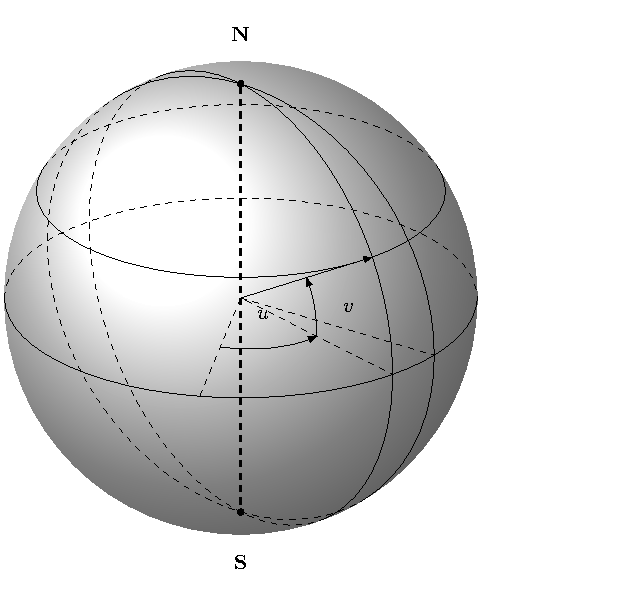
\includegraphics[width=0.45\linewidth, keepaspectratio]{figures/spherical-coordinates.pdf}
                    \label{fig:spherical-coordinates}
                }%
                \subfloat[Rotationskörper]{
                    \resizebox{0.45\linewidth}{!}{% Author: Marco Miani
\documentclass[varwidth=true, border=2pt]{standalone}

\usepackage{pgfplots}
\pgfplotsset{compat=1.9}

\begin{document}
    \pgfplotsset{
        colormap={whitered}{
            color(0cm)=(white);
            color(1cm)=(orange!75!red)
        }
        %colormap={color}{color(0cm)=(white); color(1cm)=(blue)}
    }
    \begin{tikzpicture}
     \begin{axis}[view={60}{30}]
      \addplot3[surf,
      samples=50,
      domain=1:2,y domain=0:2*pi,
      z buffer=sort]
      %({(2 + tan(deg(y)))*cos((deg(x)))}, {(2 + cos(x)) * sin(x)}, {x});
      ({x * cos(deg(y))}, {x * sin(deg(y))}, {1/x});
     \end{axis}
    \end{tikzpicture}
\end{document}
}
                    \label{fig:solid-of-revolution}
                }%

                \subfloat[Sinus und Kosinus haben keine gemeinsame Nullstelle]{
                    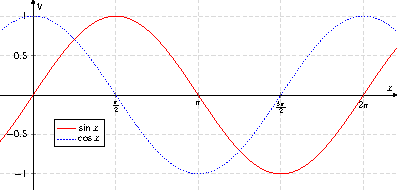
\includegraphics[width=0.8\linewidth, keepaspectratio]{figures/sin-cos.pdf}
                    \label{fig:sin-cos}
                }%
                \label{fig:example-image-gallery-1}
                %\caption{}
            \end{figure}

            \[J_F(u,v) = 
            \begin{pmatrix}
                -r(v) \sin u & r'(v) \cos u\\
                r(v) \cos u  & r'(v) \sin u\\
                 0           & 1
            \end{pmatrix}\]
            hat Rang 2 für alle $(u,v) \in \mdr^2$.
        \item Kugelkoordinaten: $F: \mdr^2 \rightarrow \mdr^3$,\\
              $(u, v) \mapsto (R \cos v \cos u, R \cos v \sin u, R \sin v)$\\
              Es gilt: $F(u,v) \in S_R^2$, denn 
                \begin{align*}
                    & R^2 \cos^2(v) \cos^2(u) + R^2 \cos^2(v) \sin^2(u) + R^2 \sin^2(v)\\
                    =& R^2 (\cos^2(v) \cos^2(u) + \cos^2(v) \sin^2(u) + \sin^2(v))\\
                    =& R^2 \left (\cos^2(v) (\cos^2(u) + \sin^2(u)) + \sin^2(v) \right)\\
                    =& R^2 \left (\cos^2(v) + \sin^2(v) \right)\\
                    =&R^2
                \end{align*}

                Die Jacobi-Matrix
                \[J_F(u,v) = 
                \begin{pmatrix}
                    -R \cos v \sin u & -R \sin v \cos u\\
                    R \cos v \cos u  & -R \sin v \sin u\\
                    0                & R \cos v
                \end{pmatrix}\]
                hat Rang 2 für $\cos v \neq 0$. In $N$ und $S$ ist
                $\cos v = 0$.
    \end{bspenum}
\end{beispiel}

%%%%%%%%%%%%%%%%%%%%%%%%%%%%%%%%%%%%%%%%%%%%%%%%%%%%%%%%%%%%%%%%%%%%%
% Mitschrieb vom 21.11.2013                                         %
%%%%%%%%%%%%%%%%%%%%%%%%%%%%%%%%%%%%%%%%%%%%%%%%%%%%%%%%%%%%%%%%%%%%%
\begin{bemerkung}\label{kor:regular-surface-mannigfaltigkeit}
    Jede reguläre Fläche $S \subseteq \mdr^3$ ist eine 2-dimensionale,
    differenzierbare Mannigfaltigkeit.
\end{bemerkung}

\begin{beweis}
    \todo{Hier muss ich nochmals drüber lesen.}
    \underline{z.Z.:} $F_j^{-1} \circ F_i$ ist Diffeomorphismus

    \begin{figure}[htp]
        \centering
        \documentclass[varwidth=true, border=2pt]{standalone}
\usepackage{amsmath,amssymb}% math symbols / fonts
\usepackage{tikz}
\usepackage{tqft}
\usetikzlibrary{patterns}

\begin{document}
    \begin{tikzpicture}
        \tikzstyle{point}=[circle,thick,draw=black,fill=black,inner sep=0pt,minimum width=2pt,minimum height=2pt]
        \draw (0,0) ellipse (2cm and 1cm);
        \def\ringa{(-0.3,0) circle (0.5cm)}
        \def\ringb{(+0.3,0) circle (0.5cm)}

        \draw \ringa;
        \draw[red] \ringb;

        %\node at (-1,0.3) {$U_i$};
        %\node at (+1,0.3) {$U_j$};
        \node at (-1.9,-2) {$U_i$};
        \node[red] at (+1.9,-2) {$U_j$};
        \node at (+2.0,0.7) {$S$};
        \node[point,label={[label distance=-0.1cm]90:$s$}] at (0,0) {};


        \path[<-] (-0.35,0)  edge [bend angle=10,bend right] node[label={[label distance=0.1cm]210:$F_i$}] {} (-1,-1.5);
        \path[<-,red] (+0.35,0)  edge [bend angle=10,bend left]  node[label={[label distance=0.1cm]-30:$F_j$}] {} (+1,-1.5);

        \draw (-1,-2) circle (0.5cm);
        \draw[red] (+1,-2) circle (0.5cm);

        \path[->, green, thick] (-0.3,-2) edge node[label=below:$\scriptstyle F_j^{-1} \circ F_i$] {} (0.3,-2);
    \end{tikzpicture}
\end{document}

        \caption{Reguläre Fläche $S$ zum Beweis von \cref{kor:regular-surface-mannigfaltigkeit}}
        \label{fig:parametric-surface-mapping}
    \end{figure}
    

    \underline{Idee:} Finde differenzierbare Funktion $\widetilde{F_j^{-1}}$
    in Umgebung $W$ von $s$, sodass $\widetilde{F_j^{-1}}|_{S \cap W} = F_j^{-1}$.

    \underline{Ausführung:} Sei $u_0 \in U_i$ mit $F_i(u_0) = s = F_j(v_0), v_0 \in U_j$.

    Da $\rang(J_{F_j}(v_0)) = 2$ ist, ist \obda 
    \[\det 
        \begin{pmatrix}
            \frac{\partial x}{\partial u} & \frac{\partial x}{\partial v}\\
            \frac{\partial y}{\partial u} & \frac{\partial y}{\partial v}
        \end{pmatrix} (v_0) \neq 0
    \]

    und $F_j(u,v) = \left ( x(u,v), y(u,v), z(u,v) \right)$.

    Definiere $\widetilde{F_j}: U_j \times \mdr \rightarrow \mdr^3$ durch
    \[\widetilde{F_j} (u, v, t) = \left(x(u,v), y(u,v), z(u,v)+t \right )\]
    
    Offensichtlich: $\widetilde{F_j} |_{U_j \times \Set{0}} = F_j$

    \[J_{\widetilde{F_j}} = 
    \begin{pmatrix}
        \frac{\partial x}{\partial u}   & \frac{\partial x}{\partial v} & 0\\
        \frac{\partial y}{\partial u}   & \frac{\partial y}{\partial v} & 0\\
        \frac{\partial z}{\partial u}   & \frac{\partial z}{\partial v} & 1
    \end{pmatrix} \Rightarrow \det J_{\widetilde{F_j}} (v_0, 0) \neq  0\]

    $\xRightarrow{\text{Analysis II}}$ Es gibt Umgebungen $W$ von
    $F_j$ von $\widetilde{F_j}(v_0, 0) = F_j(v_0) = s$, sodass $\widetilde{F_j}$
    auf $W$ eine differenzierbar Inverse $F_j^{-1}$ hat.

    Weiter ist $\widetilde{F_j}^{-1}|_{W \cap S} = F_j^{-1} |_{W \cap S}$
    $\Rightarrow F_j^{-1} \circ F_i |_{F_i^{-1} (W \cap S)} = F_j^{-1} \circ F_i |_{F_i^{-1} (W \cap S)}$
    ist differenzierbar.
\end{beweis}

\begin{definition}%
    Sei $G$ eine Mannigfaltigkeit, $\circ: G \times G \rightarrow G$
    eine Abbildung, $(g,h) \mapsto g \cdot h$, sodass $(G, \circ)$
    eine Gruppe ist.

    \begin{defenum}
        \item $G$ heißt \textbf{topologische Gruppe}\xindex{Gruppe!topologische},
              wenn die Abbildungen $\circ: G \times G \rightarrow G$
              und $\iota: G \rightarrow G$.
              \[(g, h) \mapsto g \cdot h\;\;\; g \mapsto g^{-1}\]
              stetig sind.
        \item Ist $G$ eine differenzierbare Mannigfaltigkeit, so heißt
              $G$ \textbf{Lie-Gruppe}\xindex{Lie-Gruppe}, wenn
              $(G, \circ)$ und $(G, \iota)$ differenzierbar sind.
    \end{defenum}
\end{definition}

\begin{beispiel}[Lie-Gruppen]
    \begin{bspenum}
        \item Alle endlichen Gruppen sind 0-dimensionale Lie-Gruppen.
        \item $\GL_n(\mdr)$
        \item $(\mdr^\times, \cdot)$
        \item $(\mdr_{>0}, \cdot)$
        \item $(\mdr^n, +)$, denn $A \cdot B (i,j) = \sum_{k=1}^n a_{ik} b_{kj}$ ist
              nach allen Variablen differenzierbar

              $(A^{-1}) (i,j) = \frac{\det(A_{ij})}{\det A}$

              \[A_{ij} = \begin{pmatrix}
                a_{i1} & \dots  & a_{in}\\
                \vdots & \ddots & \vdots\\
                a_{n1} & \dots  & a_{nn}
              \end{pmatrix} \in \mdr^{(n-1) \times (n-1)}\]

            ist differenzierbar.

            $\det A_{ij}$ kann $0$ werden, da:
            \[\begin{pmatrix}1 & 1\\-1&0\end{pmatrix}\]
        \item $\SL_n(\mdr) = \Set{A \in \GL_n(\mdr) | \det(A) = 1} $ \todo{Besser strukturieren}

              $\grad(\det-1)(A) = 0$?

              $\frac{\partial}{\partial a_{11}} (\det -1) = 1 \cdot \det A_{11}$

              Es gibt $i \in \Set{1, \dots, n}$ mit $\frac{\partial}{\partial a_{1i}} (\det -1) A \neq 0$
    \end{bspenum}
\end{beispiel}

\begin{bemerkung}
    Ist $G$ eine Lie-Gruppe, $g \in G$, so ist die Abbildung
    \begin{align*}
        l_g &: G \rightarrow G\\
        h  &\mapsto g \cdot h
    \end{align*}

    ein Diffeomorphismus.
\end{bemerkung}

\section{Simplizialkomplex}
\begin{definition}\xindex{Lage!allgemeine}%
    Seien $v_0, \dots, v_k \in \mdr^n$ Punkte.
    \begin{defenum}
        \item $v_0, \dots, v_k$ sind \textbf{in allgemeiner Lage} $\gdw$ es gibt keinen $(k-1)$-dimensionalen
              affinen Untervektorraum, der $v_0, \dots, v_k$ enthält
              \gdw $v_1 - v_0, \dots, v_k - v_0$ sind linear unabhängig.
        \item $\conv(v_0, \dots, v_k) := \Set{\sum_{i=0}^k \lambda_i v_i | \lambda_i \geq 0, \sum_{i=0}^k \lambda_i = 1} $
    \end{defenum}
\end{definition}

\begin{definition}
    \begin{defenum}
        \item Sei $\Delta^k = \conv(e_0, \dots, e_k) \subseteq \mdr^{n+1}$
              die konvexe Hülle der Standard-Basisvektoren $e_0, \dots, e_k$.

              Dann heißt $\Delta^k$ \textbf{Standard-Simplex}\xindex{Standard-Simplex}
              und $k$ die Dimension des Simplex.
        \item Für Punkte $v_0, \dots, v_k$ im $\mdr^n$ in allgemeiner
              Lage heißt $\delta (v_0, \dots, v_k) = \conv(v_0, \dots, v_k)$
              ein \textbf{$k$-Simplex}\xindex{Simplex} in $\mdr^n$.
        \item Ist $\Delta (v_0, \dots, v_k)$ ein $k$-Simplex und
              $I = \Set{i_0, \dots, i_r} \subseteq \Set{0, \dots, k}$,
              so heißt $s_{i_0, \dots, i_r} := \conv(v_{i_0}, \dots, v_{i_r})$
              \textbf{Teilsimplex}\xindex{Teilsimplex} oder \textbf{Seite}\xindex{Seite}
              von $\Delta$. 

              $s_{i_0, \dots, i_r}$ ist $r$-Simplex.
    \end{defenum}
\end{definition}

\begin{figure}[ht]
    \centering
    \subfloat[0-Simplex $\Delta^0$]{
        \parbox{5cm}{\centering\documentclass[varwidth=true, border=2pt]{standalone}

\usepackage{tikz}
\usepackage{amsmath,amssymb}

\begin{document}
    \begin{tikzpicture}[thick]
        \draw[thick, fill=black, black] (0cm,0cm) circle(0.1cm);
        %\node[below] {$1$};
    \end{tikzpicture}
\end{document}
}
        \label{fig:simplex-0}
    }

    \subfloat[1-Simplex $\Delta^1$]{
        \documentclass[varwidth=true, border=2pt]{standalone}

\usepackage{pgfplots}
\usepackage{tikz}
\usepackage{tkz-fct}
\usetikzlibrary{shapes.misc}

\begin{document}
\begin{tikzpicture}
    \tikzstyle{point}=[thick,draw=black,cross out,inner sep=0pt,minimum width=4pt,minimum height=4pt]
    \begin{axis}[
        legend pos=south west,
        axis x line=middle,
        axis y line=middle,
        grid = major,
        width=5cm,
        height=5cm,
        grid style={dashed, gray!30},
        xmin=0,    % start the diagram at this x-coordinate
        xmax=3,    % end   the diagram at this x-coordinate
        ymin=0,    % start the diagram at this y-coordinate
        ymax=3,    % end   the diagram at this y-coordinate
        %xlabel=$x$,
        %ylabel=$y$,
        tick align=outside,
        minor tick num=-3,
        enlargelimits=true,
        tension=0.08]
      \addplot[domain=0:2.5, red, thick,samples=20] {-x+2.5};
      \node[point,label={[label distance=0cm]45:$e_0$}] at (axis cs:2.5,0) {};
      \node[point,label={[label distance=0cm]0:$e_1$}] at (axis cs:0,2.5) {};
    \end{axis} 
\end{tikzpicture}
\end{document}

        \label{fig:simplex-1}
    }%
    \subfloat[2-Simplex $\Delta^2$]{
        \documentclass[varwidth=true, border=2pt]{standalone}

\usepackage{pgfplots}
\usepackage{tikz}
\usepackage{tkz-fct}
\usetikzlibrary{shapes.misc}

\begin{document}
\begin{tikzpicture}
    \tikzstyle{point}=[thick,draw=black,cross out,inner sep=0pt,minimum width=4pt,minimum height=4pt]
    \begin{axis}[
        legend pos=south west,
        axis x line=middle,
        axis y line=middle,
        grid = major,
        width=5cm,
        height=5cm,
        grid style={dashed, gray!30},
        xmin=0,    % start the diagram at this x-coordinate
        xmax=3,    % end   the diagram at this x-coordinate
        ymin=0,    % start the diagram at this y-coordinate
        ymax=3,    % end   the diagram at this y-coordinate
        tick align=outside,
        minor tick num=-3,
        enlargelimits=true,
        tension=0.08]
        \node (a)[point,label={[label distance=0cm]5:$e_0$}] at (axis cs:2.5,0) {};
        \node (b)[point,label={[label distance=0cm]5:$e_1$}] at (axis cs:0,2.5) {};
        \node (c)[point,label={[label distance=0cm]0:$e_2$}] at (axis cs:2,2) {};
        \draw[thick,fill=orange!50] (a.center) -- (b.center) -- (c.center) -- cycle;
    \end{axis} 
\end{tikzpicture}
\end{document}

        \label{fig:simplex-2}
    }%
    \subfloat[3-Simplex $\Delta^3$]{
        \begin{tikzpicture}
    \tikzstyle{point}=[thick,draw=black,cross out,inner sep=0pt,minimum width=4pt,minimum height=4pt]

    \node (a)[point,label={[label distance=0cm]180:$e_0$}] at (0,0) {};
    \node (b)[point,label={[label distance=0cm]0:$e_1$}] at (2,0) {};
    \node (c)[point,label={[label distance=0cm]0:$e_2$}] at (1,2) {};
    \node (d)[point,label={[label distance=0cm]0:$e_3$}] at (1,0.7) {};
    \draw (a.center) -- (b.center) -- (c.center) -- cycle;
    \draw[dashed] (a.center) -- (d.center) -- (b.center);
    \draw[dashed] (d.center) -- (c.center);
\end{tikzpicture}

        \label{fig:simplex-3}
    }%
    \label{fig:k-simplexe}
    \caption{Beispiele für $k$-Simplexe}
\end{figure}


%%%%%%%%%%%%%%%%%%%%%%%%%%%%%%%%%%%%%%%%%%%%%%%%%%%%%%%%%%%%%%%%%%%%%
% Mitschrieb vom 21.11.2013                                         %
%%%%%%%%%%%%%%%%%%%%%%%%%%%%%%%%%%%%%%%%%%%%%%%%%%%%%%%%%%%%%%%%%%%%%
\begin{definition}%
    \begin{enumerate}[label=\alph*),ref=\thedefinition.\alph*]
        \item Eine endliche Menge $K$ von Simplizes im $\mdr^n$
              heißt (endlicher) \textbf{Simplizialkomplex}\xindex{Simplizialkomplex},
              wenn gilt:
            \begin{enumerate}[label=(\roman*),ref=\theenumii.\roman*]
                \item Für $\Delta \in K$ und $S \subseteq \Delta$ Teilsimplex
                      ist $S \in K$
                \item Für $\Delta_1, \Delta_2 \in K$ ist 
                      $\Delta_1 \cap \Delta_2$ leer oder ein 
                        Teilsimplex von $\Delta_1$ und von 
                      $\Delta_2$ \label{def:simplizialkomplex.ii}
            \end{enumerate}
        \item $|K| := \bigcup_{\Delta \in K} \Delta$ (mit Teilraumtopologie)
              heißt \textbf{geometrische Realisierung}\xindex{Realisierung!geometrische}
              von $K$.
        \item Ist $d = \max \Set{ k | K \text{ enthält } k-\text{Simplex}}$,
              so heißt $d$ \textbf{Dimension}\xindex{Dimension} von
              $K$.
    \end{enumerate}
\end{definition}

\xindex{Oktaeder}\xindex{Würfel}
\begin{figure}[ht]
    \centering
    \subfloat[1D Simplizialkomplex]{
        \parbox[c][4cm]{3.5cm}{\centering\begin{tikzpicture}
    \tikzstyle{point}=[circle,thick,draw=black,fill=black,inner sep=0pt,minimum width=4pt,minimum height=4pt]
    \node (a)[point] at (0.4,0) {};
    \node (b)[point] at (1,1) {};
    \node (c)[point] at (2,1) {};
    \node (d)[point] at (2.6,0) {};
    \node (e)[point] at (2,-1) {};
    \node (f)[point] at (1,-1) {};
    \draw (a.center) -- (b.center) -- (c.center) -- (d.center) -- (e.center) -- (f.center) -- cycle;
\end{tikzpicture}
}
        \label{fig:simplizialkomplex-1-d}
    }%
    \subfloat[2D Simplizialkomplex (ohne untere Fläche!)]{
        \parbox[c][4cm]{3.5cm}{\centering\begin{tikzpicture}
    \tikzstyle{point}=[circle,thick,draw=black,fill=black,inner sep=0pt,minimum width=4pt,minimum height=4pt]
    \node (a)[point] at (0,0) {};
    \node (b)[point] at (2,0) {};
    \node (c)[point] at (3,1) {};
    \node (d)[point] at (1,1) {};
    \node (e)[point] at (1.5,3) {};
    \draw (a.center) -- (b.center) -- (c.center) -- (e.center) -- (b.center);
    \draw (a.center) -- (e.center);
    \draw[dashed] (a.center) -- (d.center) -- (c.center);
    \draw[dashed] (d.center) -- (e.center);
\end{tikzpicture}
}
        \label{fig:simplizialkomplex-2-d}
    }%
    \subfloat[2D Simplizialkomplex]{
        \parbox[c][4cm]{5cm}{\centering\begin{tikzpicture}
    \tikzstyle{point}=[circle,thick,draw=black,fill=black,inner sep=0pt,minimum width=4pt,minimum height=4pt]
    \node (a)[point] at (0,0) {};
    \node (b)[point] at (2,0) {};
    \node (c)[point] at (3,1) {};
    \node (d)[point] at (1,1) {};
    \node (e)[point] at (1.5,3) {};
    \node (f)[point] at (1.5,-1) {};
    \draw (a.center) -- (b.center) -- (c.center) -- (e.center) -- (b.center);
    \draw (a.center) -- (e.center);
    \draw[dashed] (a.center) -- (d.center) -- (c.center);
    \draw[dashed] (d.center) -- (e.center);

    \draw (a.center) -- (f.center) -- (b.center);
    \draw (f.center) -- (c.center);
    \draw[dashed] (f.center) -- (d.center);
\end{tikzpicture}
}
        \label{fig:simplizialkomplex-2-d-okateder}
    }%

    \subfloat[1D Simplizialkomplex]{
        \parbox[c][4cm]{5cm}{\centering\documentclass[varwidth=true, border=2pt]{standalone}
\usepackage{tikz}

\begin{document}
\begin{tikzpicture}
    \tikzstyle{point}=[circle,thick,draw=black,fill=black,inner sep=0pt,minimum width=4pt,minimum height=4pt]
    \node (a)[point] at (0,0) {};
    \node (b)[point] at (4,0) {};
    \node (c)[point] at (5,1) {};
    \node (d)[point] at (1,1) {};
    \node (e)[point] at (0,2) {};
    \node (f)[point] at (4,2) {};
    \node (g)[point] at (5,3) {};
    \node (h)[point] at (1,3) {};
    \draw (a.center) -- (b.center) -- (f.center) -- (e.center) -- cycle;
    \draw (b.center) -- (c.center) -- (g.center) -- (f.center) -- cycle;
    \draw (e.center) -- (f.center) -- (g.center) -- (h.center) -- cycle;
    \draw[dashed] (a.center) -- (d.center) -- (c.center);
    \draw[dashed] (d.center) -- (h.center);
\end{tikzpicture}
\end{document}
}
        \label{fig:simplizialkomplex-cube}
    }%
    \subfloat[2D Simplizialkomplex]{
        \parbox[c][4cm]{5cm}{\centering\documentclass[varwidth=true, border=2pt]{standalone}
\usepackage{tikz}

\begin{document}
\begin{tikzpicture}
    \tikzstyle{point}=[circle,thick,draw=black,fill=black,inner sep=0pt,minimum width=4pt,minimum height=4pt]
    \node (a)[point] at (0,0) {};
    \node (b)[point] at (4,0) {};
    \node (c)[point] at (5,1) {};
    \node (d)[point] at (1,1) {};
    \node (e)[point] at (0,2) {};
    \node (f)[point] at (4,2) {};
    \node (g)[point] at (5,3) {};
    \node (h)[point] at (1,3) {};
    \draw (a.center) -- (b.center) -- (f.center) -- (e.center) -- cycle;
    \draw (b.center) -- (c.center) -- (g.center) -- (f.center) -- cycle;
    \draw (e.center) -- (f.center) -- (g.center) -- (h.center) -- cycle;
    \draw[dashed] (a.center) -- (d.center) -- (c.center);
    \draw[dashed] (d.center) -- (h.center);

    \draw[orange] (b.center) -- (e.center) -- (g.center);
    \draw[orange,dashed] (a.center) -- (c.center) -- (h.center);
    \draw[orange,dashed] (d.center) -- (e.center);
    \draw[orange] (f.center) -- (c.center);

    \node (a)[point] at (0,0) {};
    \node (b)[point] at (4,0) {};
    \node (c)[point] at (5,1) {};
    \node (d)[point] at (1,1) {};
    \node (e)[point] at (0,2) {};
    \node (f)[point] at (4,2) {};
    \node (g)[point] at (5,3) {};
    \node (h)[point] at (1,3) {};
\end{tikzpicture}
\end{document}
}
        \label{fig:simplizialkomplex-cube-divided}
    }

    \subfloat[$P$ ist kein Teilsimplex, da Eigenschaft \cref{def:simplizialkomplex.ii} verletzt ist]{
        \parbox[c][4cm]{5cm}{\centering\documentclass[varwidth=true, border=2pt]{standalone}
\usepackage{tikz}
\usetikzlibrary{patterns}

\begin{document}
\begin{tikzpicture}
    \tikzstyle{point}=[circle,thick,draw=black,fill=black,inner sep=0pt,minimum width=4pt,minimum height=4pt]
    \node (a)[point] at (0,0) {};
    \node (b)[point] at (3,0) {};
    \node (c)[point] at (2,2) {};

    \begin{scope}[yshift=2cm]
    \node (d)[point] at (1,1) {};
    \node (e)[point] at (0,2) {};
    \node (f)[point] at (4,2) {};
    \end{scope}
    
    \node (p)[point,label={[label distance=0cm]5:$P$}] at (1.5,0.5) {};

    \draw[pattern=north east lines] (a.center) -- (b.center) -- (c.center) -- cycle;
    \draw[pattern=dots] (d.center) -- (e.center) -- (f.center) -- cycle;
    \draw (p.center) -- (d.center);
\end{tikzpicture}
\end{document}
}
        \label{fig:no-simplizialkomplex-triangles}
    }%
    \subfloat[Simplizialkomplex]{
        \parbox[c][4cm]{5cm}{\centering\begin{tikzpicture}
    \tikzstyle{point}=[circle,thick,draw=black,fill=black,inner sep=0pt,minimum width=4pt,minimum height=4pt]
    \node (a)[point] at (0,0) {};
    \node (b)[point] at (3,0) {};
    \node (c)[point] at (2,2) {};

    \begin{scope}[yshift=2cm]
    \node (d)[point] at (1,1) {};
    \node (e)[point] at (0,2) {};
    \node (f)[point] at (4,2) {};
    \end{scope}
    
    \node (p)[point,label={[label distance=0cm]5:$P$}] at (1.5,0.5) {};

    \draw[pattern=north east lines] (a.center) -- (p.center) -- (b.center) -- cycle;
    \draw[pattern=north west lines] (a.center) -- (p.center) -- (c.center) -- cycle;
    \draw[pattern=vertical lines]   (b.center) -- (p.center) -- (c.center) -- cycle;
    \draw[pattern=dots] (d.center) -- (e.center) -- (f.center) -- cycle;
    \draw (p.center) -- (d.center);
\end{tikzpicture}
}
        \label{fig:simplizialkomplex-triangles}
    }%
    \label{fig:simplizialkomplexe}
    \caption{Beispiele für Simplizialkomplexe}
\end{figure}

\begin{definition}\xindex{Abbildung!simpliziale}%
    Seien $K, L$ Simplizialkomplexe. Eine stetige Abbildung
    \[f:|K| \rightarrow |L|\]
    heißt \textbf{simplizial}, wenn für
    jedes $\Delta \in K$ gilt:
    \begin{defenum}
        \item $f(\Delta) \in L$
        \item $f|_{\Delta} : \Delta \rightarrow f(\Delta)$ ist eine
              affine Abbildung.
    \end{defenum}
\end{definition}

\begin{beispiel}
    \begin{bspenum}
        \item $\varphi(e_1) := b_1$, $\varphi(e_2) := b_2$\\
              $\varphi$ ist eine eindeutig bestimmte lineare Abbildung

              \begin{tikzpicture}
    \tikzstyle{point}=[circle,thick,draw=black,fill=black,inner sep=0pt,minimum width=4pt,minimum height=4pt]

    \node (a)[point,label={[label distance=0cm]180:$0$}] at (0,0) {};
    \node (b)[point,label={[label distance=0cm]0:$e_2$}] at (2.5,0) {};
    \node (c)[point,label={[label distance=0cm]90:$e_1$}] at (2,1) {};

    \begin{scope}[xshift=5cm]
        \node (d)[point,label={[label distance=0cm]180:$0$}] at (0,0) {};
        \node (e)[point,label={[label distance=0cm]0:$b_1$}] at (4,0) {};
        \node (f)[point,label={[label distance=0cm]90:$b_2$}] at (2,2) {};
    \end{scope}

    \draw (a.center) -- (b.center) -- (c.center) -- cycle;
    \draw (d.center) -- (e.center) -- (f.center) -- cycle;

    \draw[thick,->] (3,0.5) -- node[above] {$\varphi$} (5,0.5);
\end{tikzpicture}


        \item Folgende Abbildung $\Delta^n \rightarrow \Delta^{n-1}$ 
              ist simplizial:

              \begin{tikzpicture}
    \tikzstyle{point}=[circle,thick,draw=black,fill=black,inner sep=0pt,minimum width=4pt,minimum height=4pt]

    \node (a)[point] at (0,0) {};
    \node (b)[point] at (2.5,0) {};
    \node (c)[point] at (2,1) {};

    \begin{scope}[xshift=4.5cm, yshift=0.5cm]
        \node (d)[point] at (0,0) {};
        \node (e)[point] at (2,0) {};
    \end{scope}

    \begin{scope}[xshift=1.5cm,yshift=0.6cm,rotate=-55]
    \draw[->] (0,-0.1) -- (0.4,-0.1);
    \draw[->] (0, 0.0) -- (0.5, 0.0);
    \draw[->] (0, 0.1) -- (0.6, 0.1);
    \end{scope}

    \draw (a.center) -- (b.center) -- (c.center) -- cycle;
    \draw (d.center) -- (e.center);

    \draw[thick,->] (3,0.5) -- node[above] {$\varphi$} (4,0.5);
\end{tikzpicture}

        \item \todo[inline]{Wozu dient das Beispiel?}

            \resizebox{0.9\linewidth}{!}{\begin{tikzpicture}[scale=1.5]
    \tikzstyle{point}=[circle,thick,draw=black,fill=black,inner sep=0pt,minimum width=4pt,minimum height=4pt]
    \node (a)[point] at (0,0) {};
    \node (b)[point] at (1,0) {};
    \node (c)[point] at (2,0) {};

    \node (d)[point] at (0,1) {};
    \node (M)[point,label={[label distance=0cm]5:$M$}] at (1,1) {};
    \node (f)[point] at (2,1) {};

    \node (g)[point] at (0,2) {};
    \node (h)[point] at (1,2) {};
    \node (i)[point] at (2,2) {};

    \draw (a.center) -- node[below] {$a$} (b.center);
    \draw (b.center) -- node[below] {$b$} (c.center);
    \draw (g.center) -- node[above] {$a$} (h.center);
    \draw (h.center) -- node[above] {$b$} (i.center);
    \draw (d.center) -- node[left] {$c$} (g.center);
    \draw (d.center) -- node[left] {$d$} (a.center);
    \draw (f.center) -- node[right] {$d$} (c.center);
    \draw (i.center) -- node[right] {$c$} (f.center);

    \draw (a.center) -- (b.center) -- (M.center) -- (d.center) -- cycle;
    \draw (b.center) -- (c.center) -- (f.center) -- (M.center) -- cycle;
    \draw (d.center) -- (M.center) -- (h.center) -- (g.center) -- cycle;
    \draw (M.center) -- (f.center) -- (i.center) -- (h.center) -- cycle;

    \draw[thick, blue] (d.center) -- (M.center) -- (f.center);

    \draw[thick, red] (a.center) -- (b.center);
    \draw[thick, red] (h.center) -- (i.center);

    % Draw again so that lines are below nodes
    \draw (a.center) -- (i.center);
    \draw (c.center) -- (g.center);

    \node (a)[point] at (0,0) {};
    \node (b)[point] at (1,0) {};
    \node (c)[point] at (2,0) {};

    \node (d)[point] at (0,1) {};
    \node (M)[point,label={[label distance=0cm]5:$M$}] at (1,1) {};
    \node (f)[point] at (2,1) {};

    \node (g)[point] at (0,2) {};
    \node (h)[point] at (1,2) {};
    \node (i)[point] at (2,2) {};

    \draw[->] (3,1) -- node[above] {Quotient nach} node[below] {Punktspiegelung} (5,1);

    \begin{scope}[xshift=6.5cm,yshift=1cm]
        \node (w)[point] at (-1,0) {};
        \node (x)[point] at (0,-1) {};
        \node (y)[point] at (1,0) {};
        \node (z)[point] at (0,1) {};
        \node (m)[point] at (0,0) {};

        \node (1) at (-0.3,+0.35) {1};
        \node (2) at (+0.3,+0.35) {2};
        \node (3) at (+0.3,-0.35) {3};
        \node (4) at (-0.3,-0.35) {4};

        \draw (w.center) -- (x.center) -- (y.center) -- (z.center) -- cycle;

        \draw[thick, blue] (w.center) -- (m.center);
        \draw (m.center) -- (y.center);
        \draw (x.center) -- (m.center) -- (z.center);
        \draw[thick, red] (z.center) -- (y.center) -- (x.center);

        % Draw again, as lines should be below points
        \node (w)[point] at (-1,0) {};
        \node (x)[point] at (0,-1) {};
        \node (y)[point] at (1,0) {};
        \node (z)[point] at (0,1) {};
        \node (m)[point] at (0,0) {};
    \end{scope}
\end{tikzpicture}
}
    \end{bspenum}
\end{beispiel}

\begin{definition}\xindex{Eulerzahl}%
    Sei $K$ ein endlicher Simplizialkomplex. Für $n \geq 0$ sei
    $a_n(K)$ die Anzahl der $n$-Simplizes in $K$.

    Dann heißt 
    \[\chi(K) := \sum_{n=0}^{\dim K} (-1)^n a_n(K)\]
    \textbf{Eulerzahl} (oder Euler-Charakteristik\index{Euler-Charakteristik|see{Eulerzahl}})
    von $K$.
\end{definition}

\begin{beispiel}
    \begin{bspenum}
        \item $\chi(\Delta^1) = 2 - 1 = 1$\\
              $\chi(\Delta^2) = 3 - 3 + 1 = 1$\\
              $\chi(\Delta^3) = 4 - 6 + 4 - 1 = 1$
        \item $\chi(\text{Oktaeder-Oberfläche}) = 6 - 12 + 8 = 2$\\
              $\chi(\text{Rand des Tetraeders}) = 2$\\
              $\chi(\text{Ikosaeder}) = 12 - 30 + 20 = 2$
        \item $\chi(\text{Würfel}) = 8 - 12 + 6 = 2$\\
              $\chi(\text{Würfel, unterteilt in Dreiecksflächen}) = 8 - (12 + 6) + (6 \cdot 2) = 2$
    \end{bspenum}
\end{beispiel}

\begin{bemerkung}
    $\chi(\Delta^n) = 1$ für jedes $n \in \mdn_0$
\end{bemerkung}

\begin{beweis}
    $\Delta^n$ ist die konvexe Hülle von $(e_0, \dots, e_n)$ in $\mdr^{n+1}$.
    Jede $(k+1)$-elementige Teilmenge von $\Set{e_0, \dots, e_n}$
    definiert ein $k$-Simplex.\\
    $\Rightarrow a_k(\Delta^n) = \binom{n+1}{k+1}, \;\;\; k = 0, \dots, n$\\
    $\Rightarrow \chi(\Delta^n) = \sum_{k=0}^n (-1)^k \binom{n+1}{k+1}$\\
    $f(x) = (x+1)^{n+1} \overset{\substack{\text{\tiny{Binomischer}}\\\text{\tiny{Lehrsatz}}}}{=} \sum_{k=0}^{n+1} \binom{n+1}{k} x^k$\\
    $\Rightarrow 0 = \sum_{k=0}^{n+1} \binom{n+1}{k} (-1)^k = \chi(\Delta^n) -1$\\
    $\Rightarrow \chi(\Delta^n) = 1 \qed$
\end{beweis}

%%%%%%%%%%%%%%%%%%%%%%%%%%%%%%%%%%%%%%%%%%%%%%%%%%%%%%%%%%%%%%%%%%%%%
% Mitschrieb vom 28.11.2013                                         %
%%%%%%%%%%%%%%%%%%%%%%%%%%%%%%%%%%%%%%%%%%%%%%%%%%%%%%%%%%%%%%%%%%%%%
\begin{definition}%
    \begin{defenum}
        \item Ein 1D-Simplizialkomplex heißt \textbf{Graph}\xindex{Graph}.
        \item Ein Graph, der homöomorph zu $S^1$ ist, heißt \textbf{Kreis}\xindex{Kreis}.
        \item Ein zusammenhängender Graph heißt \textbf{Baum}\xindex{Baum},
              wenn er keinen Kreis enthält.
    \end{defenum}
\end{definition}

\begin{figure}[ht]
    \centering
    \subfloat[Dies wird häufig auch als Multigraph bezeichnet.]{
        \parbox[c][3cm]{4cm}{\centering\documentclass[varwidth=true, border=2pt]{standalone}
\usepackage{tikz}

\begin{document}
\begin{tikzpicture}
    \tikzstyle{point}=[circle,thick,draw=black,fill=black,inner sep=0pt,minimum width=4pt,minimum height=4pt]
    \node (a)[point] at (0,0) {};
    \node (b)[point] at (1,0) {};
    \path (a.center) edge [bend left]  (b.center);
    \path (a.center) edge              (b.center);
    \path (a.center) edge [bend right] (b.center);
\end{tikzpicture}
\end{document}
}
        \label{fig:topology-graph-simple}
    }%
    \subfloat[Planare Einbettung des Tetraeders]{
        \parbox[c][3cm]{4cm}{\centering\begin{tikzpicture}
    \tikzstyle{point}=[circle,thick,draw=black,fill=black,inner sep=0pt,minimum width=4pt,minimum height=4pt]
    \node (z)[point] at (0,0) {};
    \node (a)[point] at (90:1cm) {};
    \node (b)[point] at (210:1cm) {};
    \node (c)[point] at (330:1cm) {};
    \path (z.center) edge (a.center);
    \path (z.center) edge (b.center);
    \path (z.center) edge (c.center);
    \draw (a.center) -- (b.center) -- (c.center) -- cycle;
\end{tikzpicture}
}
        \label{fig:topology-graph-tetraeder}
    }

    \subfloat[$K_5$]{
        \parbox[c][3cm]{4cm}{\centering    \newcommand\n{5}
    \begin{tikzpicture}
        \tikzstyle{point}=[circle,thick,draw=black,fill=black,inner sep=0pt,minimum width=4pt,minimum height=4pt]

        \begin{scope}[rotate=17]
        %the multiplication with floats is not possible. Thus I split the loop in two.
        \foreach \number in {1,...,\n}{
            \node[point] (N-\number) at ({\number*(360/\n)}:1.5cm) {};
        }

        \foreach \number in {1,...,\n}{
            \foreach \y in {1,...,\n}{
                \draw (N-\number) -- (N-\y);
            }
        }
        \end{scope}
    \end{tikzpicture}
}
        \label{fig:k-5}
    }%
    \subfloat[$K_{3,3}$]{
        \parbox[c][3cm]{4cm}{\centering\documentclass[varwidth=true, border=2pt]{standalone}
\usepackage{tikz}

\begin{document}
    \begin{tikzpicture}
        \tikzstyle{point}=[circle,thick,draw=black,fill=black,inner sep=0pt,minimum width=4pt,minimum height=4pt]

        \foreach \x in {0,1,2}
        \foreach \y in {0,1,2}{
          \node (a)[point] at (\y,0) {};
          \node (b)[point] at (\x,1) {};
            \draw (a) -- (b);
        }
    \end{tikzpicture}
\end{document}
}
        \label{fig:k-3-3}
    }%
    \label{fig:graphen-beispiele}
    \caption{Beispiele für Graphen}
\end{figure}

\begin{bemerkung}
    Für jeden Baum $T$ gilt $\gamma(T) = 1$.
\end{bemerkung}

\begin{beweis}
    Induktion über die Anzahl der Ecken.
\end{beweis}

\begin{bemerkung}
    \begin{bemenum}
        \item Jeder zusammenhängende Graph $\Gamma$ enthält einen
              Teilbaum $T$, der alle Ecken von $\Gamma$ enthält.%
              \footnote{$T$ wird \enquote{Spannbaum} genannt.}
        \item Ist $n = a_1(\Gamma) = a_1(T)$, so ist $\chi(\Gamma) = 1 - n$.
    \end{bemenum}
\end{bemerkung}

\begin{beweis}\leavevmode
    \begin{enumerate}[label=\alph*),ref=\thedefinition.\alph*]
        \item Siehe \enquote{Algorithmus von Kruskal}.
        \item $\begin{aligned}[t]\chi(\Gamma) &= a_0(\Gamma) - a_1(\Gamma)\\
                                        &= a_0(\Gamma) - (n+a_1(T))\\
                                        &= a_0(T) - a_1(T) - n\\
                                        &= \chi(T) - n\\
                                        &= 1-n
              \end{aligned}$
    \end{enumerate}
\end{beweis}

\begin{bemerkung}\label{kor:simplex-unterteilung}
    Sei $\Delta$ ein $n$-Simplex und $x \in \Delta^\circ \subseteq \mdr^n$.
    Sei $K$ der Simplizialkomplex, der aus $\Delta$ durch 
    \enquote{Unterteilung} in $x$ entsteht. Dann ist $\chi(K) = \chi(\Delta) = 1$.
\end{bemerkung}

\begin{figure}[ht]
    \centering
    \subfloat[$K$]{
        \parbox{4cm}{\centering\begin{tikzpicture}
    \tikzstyle{point}=[circle,thick,draw=black,fill=black,inner sep=0pt,minimum width=4pt,minimum height=4pt]
    \node (z)[point] at (0,0) {};
    \node (a)[point] at (90:1cm) {};
    \node (b)[point] at (210:1cm) {};
    \node (c)[point] at (330:1cm) {};
    \path (z.center) edge (a.center);
    \path (z.center) edge (b.center);
    \path (z.center) edge (c.center);
    \draw (a.center) -- (b.center) -- (c.center) -- cycle;

    \draw[pattern=north west lines] (a.center) -- (b.center) -- (z.center) --cycle;
    \draw[pattern=dots] (b.center) -- (c.center) -- (z.center) --cycle;
    \draw[pattern=crosshatch] (a.center) -- (c.center) -- (z.center) --cycle;
\end{tikzpicture}
}
        \label{fig:topology-simplizial-complex-k}
    }%
    \subfloat[$\Delta$, das aus $K$ durch Unterteilung entsteht]{
        \parbox{4cm}{\centering\begin{tikzpicture}
    \tikzstyle{point}=[circle,thick,draw=black,fill=black,inner sep=0pt,minimum width=4pt,minimum height=4pt]
    \node (z)[point] at (0,0) {};
    \node (a)[point] at (90:1cm) {};
    \node (b)[point] at (210:1cm) {};
    \node (c)[point] at (330:1cm) {};
    \node (d)[point] at (10:1.5cm) {};
    \path (z.center) edge (a.center);
    \path (z.center) edge (b.center);
    \path (z.center) edge (c.center);
    \draw (a.center) -- (b.center) -- (c.center) -- cycle;

    \draw (a.center) -- (d.center);
    \draw (c.center) -- (d.center);
\end{tikzpicture}
}
        \label{fig:topology-simplizial-complex-k-division}
    }%
    \label{fig:simplex-unterteilung-beispiel}
    \caption{Beispiel für \cref{kor:simplex-unterteilung}.}
\end{figure}

\begin{beweis}
    $\chi(K) = \chi(\Delta) - \underbrace{\underbrace{(-1)^n}_{n-\text{Simplex}} + \sum_{k=0}^n (-1)^k}_{(1+(-1))^{n+1}} = \chi(\Delta) \qed$
\end{beweis}

\begin{satz}[Eulersche Polyederformel]\xindex{Eulersche Polyederformel}%
    Sei $P$ ein konvexes Polyeder in $\mdr^3$, d.~h. $\partial P$ ist
    ein 2-dimensionaler Simplizialkomplex, sodass gilt:
    \[\forall x,y \in \partial P: [x,y] \subseteq P\]

    Dann ist $\chi(\partial P) = 2$.
\end{satz}

\begin{beweis}\leavevmode
    \begin{enumerate}[label=\arabic*)]
        \item Die Aussage ist richtig für den Tetraeder.
        \item \Obda{} sei $0 \in P$ und $P \subseteq \fB_1(0)$. Projeziere
              $0P$ von $0$ aus auf $\partial \fB_1(0) = S^2$.
              Erhalte Triangulierung von $S^2$.
        \item Sind $P_1$ und $P_2$ konvexe Polygone und $T_1, T_2$
              die zugehörigen Triangulierungen von $S^2$, so gibt es 
              eine eine Triangulierungen $T$, die sowohl um $T_1$ als
              auch um $T_2$ Verfeinerung ist.

              \begin{center}
                  \centering
                  \newenvironment{customlegend}[1][]{%
    \begingroup
    % inits/clears the lists (which might be populated from previous
    % axes):
    \csname pgfplots@init@cleared@structures\endcsname
    \pgfplotsset{#1}%
}{%
    % draws the legend:
    \csname pgfplots@createlegend\endcsname
    \endgroup
}%

% makes \addlegendimage available (typically only available within an
% axis environment):
\def\addlegendimage{\csname pgfplots@addlegendimage\endcsname}

%%--------------------------------

% definition to insert numbers
\pgfkeys{/pgfplots/number in legend/.style={%
        /pgfplots/legend image code/.code={%
            \node at (0.295,-0.0225){#1};
        },%
    },
}

\pgfdeclarelayer{background}
\pgfdeclarelayer{foreground}
\pgfsetlayers{background,main,foreground}
\begin{tikzpicture}
    \tkzSetUpPoint[shape=circle,size=10,color=black,fill=black]

    \tkzDefPoints{0/0/A, 2/0/B, 3/0.5/C, 0/3/D, 2/3/E, 3/1.5/F, 2/2/G, 1/1.5/H}

    \begin{pgfonlayer}{foreground}
        %Get intersections
        \tkzInterLL(B,H)(A,C) \tkzGetPoint{I}
        \tkzInterLL(B,F)(A,C) \tkzGetPoint{J}
        \tkzInterLL(A,G)(B,H) \tkzGetPoint{K}
        \tkzInterLL(A,G)(H,F) \tkzGetPoint{L}
        \tkzInterLL(C,G)(B,F) \tkzGetPoint{M}
        \tkzInterLL(C,G)(H,F) \tkzGetPoint{N}
        \tkzInterLL(G,D)(H,E) \tkzGetPoint{O}

        \tkzDrawPoints[color=green,fill=green](A,C,G,D)
        \tkzDrawPoints[color=blue,fill=blue](B,F,E,H)
        \tkzDrawPoints[color=red,fill=red](I,J,K,L,M,N,O)
    \end{pgfonlayer}

    \tkzDrawPolygon[blue,very thick](H,E,F,B)
    \tkzDrawSegment[blue,very thick](H,F)

    \tkzDrawPolygon[green,very thick](A,D,G,C)
    \tkzDrawSegment[green,very thick](A,G)

    \tkzDrawSegments[red,very thick](I,M I,N I,L A,H H,D L,O N,E G,E)

    % \tkzLabelPoint(A){A}
    % \tkzLabelPoint(B){B}
    % \tkzLabelPoint(C){C}
    % \tkzLabelPoint(D){D}
    % \tkzLabelPoint(E){E}
    % \tkzLabelPoint(F){F}
    % \tkzLabelPoint(G){G}
    % \tkzLabelPoint(H){H}
    % \tkzLabelPoint(I){I}
    % \tkzLabelPoint(J){J}
    % \tkzLabelPoint(K){K}
    % \tkzLabelPoint(L){L}
    % \tkzLabelPoint(M){M}
    % \tkzLabelPoint(N){N}
    % \tkzLabelPoint(O){O}

    \begin{customlegend}[
    legend entries={
        $T_1$,
        $T_2$,
        $T$
    },
    legend style={at={(4.5,3.5)},font=\footnotesize}] % <= to define position and font legend
    % the following are the "images" and numbers in the legend
        \addlegendimage{blue,very thick}
        \addlegendimage{green,very thick}
        \addlegendimage{red,very thick}
    \end{customlegend}
\end{tikzpicture}\todo{Was bedeutet diese Zeichnung?}
              \end{center}

              Nach \cref{kor:simplex-unterteilung} ist
              $\chi(\partial P_1) = \chi(T_1) = \chi(T) = \chi(T_2) = \chi(\partial P_2) = 2$,
              weil \obda{} $P_2$ ein Tetraeder ist.
    \end{enumerate}
\end{beweis}

\begin{bemerkung}[Der Rand vom Rand ist 0]\label{kor:9.11}
    Sei $K$ ein \todo{Warum in Klammern?}{(endlicher)} Simplizialkomplex mit Knotenmenge $V$
    und $<$ eine Totalordnung auf $V$.

    Sei $A_n$ die Menge der $n$-Simplizes in $K$, d.~h.
    \[A_n(K) := \Set{ \sigma \in K | \dim(\sigma) = n}\;\;\; \text{für } n=0, \dots, d=\dim(K)\]

    und $C_n(K)$ der $\mdr$-Vektorraum mit Basis $A_n(K)$, d.~h.
    \[C_n(K) = \Set{\sum_{\sigma \in A_n(K)} c_\sigma \cdot \sigma | c_\sigma \in \mdr}\]

    Sei $\sigma = \Delta(x_0, \dots, x_n) \in A_n(K)$, sodass 
    $x_0 < x_1 < \dots < x_n$.

    Für $i = 0, \dots, n$ sei $\partial_i \sigma := \Delta(x_0, \dots, \hat{x_i}, \dots, x_n)$
    die $i$-te Seite von $\sigma$ und $d_\sigma = d_n \sigma := \sum_{i=0} (-1)^i \partial_i \sigma \in C_{n-1} (K)$
    und $d_n: C_n(K) \rightarrow C_{n-1}(K)$ die dadurch definierte lineare
    Abbildung.

    Dann gilt: $d_{n-1} \circ d_n = 0$
\end{bemerkung}

\begin{beispiel}
    \begin{figure}[h!]
        \centering
        \begin{tikzpicture}
    \tikzstyle{point}=[circle,thick,draw=black,fill=black,inner sep=0pt,minimum width=4pt,minimum height=4pt]
    \node (a)[point,label={[label distance=0cm]210:$a$}] at (210:1cm) {};
    \node (b)[point,label={[label distance=0cm]-45:$b$}] at (330:1cm) {};
    \node (c)[point,label={[label distance=0cm]90:$c$}] at (90:1cm) {};

    \node (sigma) at (0,0) {$\sigma$};

    \draw[->, very thick] (a) edge node[label=below:$e_3$]  {} (b);
    \draw[->, very thick] (b) edge node[label=right:$e_1$]  {} (c);
    \draw[->, very thick] (c) edge node[label=left:$e_2$]  {} (a);
\end{tikzpicture}

        \caption{Simplizialkomplex mit Totalordnung}
    \end{figure}

    $a < b < c$

    $d_2 \sigma = e_1 - e_2 + e_3 = (c - b) - (c-a) + (b - a) = 0$

    \todo[inline]{Beispiel auf Tetraeder übertragen}
\end{beispiel}

%%%%%%%%%%%%%%%%%%%%%%%%%%%%%%%%%%%%%%%%%%%%%%%%%%%%%%%%%%%%%%%%%%%%%
% Mitschrieb vom 03.12.2013                                         %
%%%%%%%%%%%%%%%%%%%%%%%%%%%%%%%%%%%%%%%%%%%%%%%%%%%%%%%%%%%%%%%%%%%%%
\begin{beweis}
    Sei $\sigma \in A_n$. Dann gilt:
    \begin{align*}
        d_{n-1}(d_n \sigma) &= d_{n-1} (\sum_{i=0}^n (-1)^i \partial_i \sigma)\\
        &= \sum_{i=0}^n (-1)^i d_{n-1} (\partial_i \sigma)\\
        &= \sum_{i=0}^n (-1)^i \sum_{j=0}^{n-1} \partial_i (\partial_j \sigma) (-1)^j\\
        &= \sum_{0 \leq i \leq j \leq n-1} (-1)^{i+j} \partial_j (\partial_j (\sigma)) + \sum_{0 \leq j < i \leq n} (-1)^{i+j} \partial_{i-1} (\partial_j \sigma)\\
        &= 0
    \end{align*}
    weil jeder Summand aus der ersten Summe auch in der zweiten
    Summe vorkommt, aber mit umgekehrten Vorzeichen. $\qed$
\end{beweis}

\begin{definition}%
    Sei $Z_n := \text{Kern}(d_n) \subseteq C_n$ und 
    $B_n := \text{Bild}(d_{n+1}) \subseteq C_n$.

    \begin{defenum}
        \item $H_n = H_n(K, \mdr) := Z_n / B_n$ heißt $n$-te 
              \textbf{Homotopiegruppe}\xindex{Homotopiegruppe} von $K$.
        \item $b_n(K) := \dim_{\mdr} H_n$ heißt $n$-te 
              \textbf{Belti-Zahl}\xindex{Belit-Zahl} von $K$.
    \end{defenum}
\end{definition}

\begin{bemerkung}
    Nach \cref{kor:9.11} ist $B_n \subseteq Z_n$, denn
    $d_{n+1}(C) \in \text{Kern}(d_n)$ für $C \in C_{n+1}$.
\end{bemerkung}

\begin{minipage}{\textwidth}%don't break this theorem!
\begin{satz}
    Für jeden endlichen Simplizialkomplex $K$ der Dimension $d$ gilt:

    \[\sum_{k=0}^d (-1)^k b_k (K) = \sum_{k=0}^d (-1)^k a_k(K) = \chi(K) \]
\end{satz}
\end{minipage}

\begin{bemerkung}
    Es gilt \underline{nicht} $a_k = b_k\;\forall k \in \mdn_0$.
\end{bemerkung}

\begin{beweis}\leavevmode
    \begin{itemize}
        \item Dimensionsformel für $d_n$: $a_n = \dim Z_n + \dim B_{n-1}$ für $n \geq 1$
        \item Dimensionsformel für $Z_n \rightarrow H_n = Z_n / B_n: \dim Z_n = b_n + \dim B_n$
    \end{itemize}

    \begin{align*}
        \Rightarrow \sum_{k=0}^d (-1)^k a_k &= a_0 + \sum_{k=1}^d (-1)^k (\dim Z_k + \dim B_{k-1})\\
        &= a_0 + \sum_{k=1}^d (-1)^k \dim Z_k + \sum_{k=0}^d (-1)^{k+1}  \dim B_{k-1}\\
        &= a_0 + \sum_{k=1}^d (-1)^k \dim Z_k - \sum_{k=0}^d (-1)^k  \dim B_{k-1}\\
        &= a_0 + \sum_{k=1}^{d-1} (-1)^k b_k + (-1)^d  \underbrace{\dim Z_d}_{= b_d} - \dim B_0\\
        &= b_0 + \sum_{k=1}^{d-1} (-1)^k b_k + (-1)^d b_d\\
        &= \sum_{k=0}^d (-1)^k b_k
    \end{align*}
\end{beweis}

% Die Übungsaufgaben sollen ganz am Ende des Kapitels sein.
\clearpage
\section*{Übungsaufgaben}
\addcontentsline{toc}{section}{Übungsaufgaben}

\begin{aufgabe}[Zusammenhang]\label{ub4:aufg1}
    \begin{enumerate}[label=(\alph*)]
        \item Beweisen Sie, dass eine topologische Mannigfaltigkeit
              genau dann wegzusammenhängend ist, wenn sie zusammenhängend
              ist
        \item Betrachten Sie nun wie in \cref{bsp:mannigfaltigkeit8}
              den Raum $X:= (\mdr \setminus \Set{0}) \cup \Set{0_1, 0_2}$
              versehen mit der dort definierten Topologie. Ist $X$
              wegzusammenhängend?
    \end{enumerate}
\end{aufgabe}


%!TEX root = GeoTopo.tex
%%%%%%%%%%%%%%%%%%%%%%%%%%%%%%%%%%%%%%%%%%%%%%%%%%%%%%%%%%%%%%%%%%%%%
% Mitschrieb vom 03.12.2013                                         %
%%%%%%%%%%%%%%%%%%%%%%%%%%%%%%%%%%%%%%%%%%%%%%%%%%%%%%%%%%%%%%%%%%%%%
\chapter{Fundamentalgruppe und Überlagerungen}
\section{Homotopie von Wegen}
\begin{figure}[ht]
    \centering
    \subfloat[$\gamma_1$ und $\gamma_2$ sind homotop, da man sie 
             \enquote{zueinander verschieben} kann.]{
        \documentclass[varwidth=true, border=2pt]{standalone}

\usepackage{pgfplots}
\usepackage{tikz}

\begin{document}
\begin{tikzpicture}
    \tikzstyle{point}=[circle,thick,draw=black,fill=black,inner sep=0pt,minimum width=4pt,minimum height=4pt]
    \node (a)[point,label=180:$a$] at (0,0) {};
    \node (b)[point,label=0:$b$]   at (3, 0) {};
    \draw [rounded corners] (a) .. controls (0.8,0.8) .. (1.5,0.8) .. controls (2.2,1) .. (b);
    \draw [rounded corners] (a) .. controls (0.6,0.6) .. (1.3,0.6) .. controls (2.0,0.8) .. (b);
    \draw [rounded corners] (a) .. controls (0.3,0.3) .. (1.0,0.3) .. controls (2.0,0.4) .. (b);
    \draw [rounded corners] (a) -- (b);
    \draw [rounded corners] (a) .. controls (1,-0.8) .. (2,-0.4) .. controls (2.2,-0.9) .. (b);
    \draw [rounded corners] (a) .. controls (1,-0.6) .. (2,-0.2) .. controls (2.2,-0.5) .. (b);
    \draw [rounded corners] (a) .. controls (1,-0.3) .. (2,-0.05) .. controls (2.2,-0.2) .. (b);
    \draw [rounded corners,->, thick, red] (a) .. controls (1,1) .. (2,1) .. controls (2.5,1) .. (b);
    \draw [rounded corners,->, thick, blue] (a) .. controls (1,-1) .. (2,-0.5) .. controls (2.2,-1) .. (b);
    \node at (1,1.2) [red] {$\gamma_1$};
    \node at (0.5,-0.8) [blue] {$\gamma_2$};
\end{tikzpicture}
\end{document}

        \label{fig:homotope-wege-anschaulich}
    }\hspace{1em}%
    \subfloat[$\gamma_1$ und $\gamma_2$ sind wegen dem Hindernis nicht homotop.]{
        \begin{tikzpicture}
    \tikzstyle{point}=[circle,thick,draw=black,fill=black,inner sep=0pt,minimum width=4pt,minimum height=4pt]
    \node (a)[point,label=180:$a$] at (0,0) {};
    \node (b)[point,label=0:$b$]   at (3, 0) {};
    \draw[orange,pattern color=orange,pattern=north east lines] (1.5,0) circle (0.3cm);
    \draw [rounded corners,->, thick, red] (a) .. controls (1,1) .. (2,1) .. controls (2.5,1) .. (b);
    \draw [rounded corners,->, thick, blue] (a) .. controls (1,-1) .. (2,-0.5) .. controls (2.2,-1) .. (b);
    \node at (1,1.2) [red] {$\gamma_1$};
    \node at (0.5,-0.8) [blue] {$\gamma_2$};
\end{tikzpicture}

        \label{fig:nicht-homotope-wege-anschaulich}
    }
    \label{fig:paths-homotop-example-counterexample}
    \caption{Beispiele für Wege $\gamma_1$ und $\gamma_2$}
\end{figure}

\begin{definition}%
    Sei $X$ ein topologischer Raum, $a, b \in X$, 
    $\gamma_1, \gamma_2: I \rightarrow X$ Wege von $a$ nach $b$,
    d.~h. $\gamma_1(0) = \gamma_2(0) = a$, $\gamma_1(1) = \gamma_2(1) = b$

    $\gamma_1$ und $\gamma_2$ heißen \textbf{homotop}\xindex{Weg!homotope},
    wenn es eine stetige Abbildung $H : I \times I \rightarrow X$ mit
    \begin{align*}
        H(t,0) &= \gamma_1(t)\;\forall t \in I\\
        H(t,1) &= \gamma_2(t)\;\forall t \in I
    \end{align*}
    und $H(0,s) = a$ und $H(1,s) = b$ für alle $s \in I$ gibt.
    Dann schreibt man: $\gamma_1 \sim \gamma_2$

    $H$ heißt \textbf{Homotopie}\xindex{Homotopie} zwischen
    $\gamma_1$ und $\gamma_2$.
\end{definition}

\begin{bemerkung}
    Sei $X$ ein topologischer Raum, $a, b \in X$, 
    $\gamma_1, \gamma_2: I \rightarrow X$ Wege von $a$ nach $b$
    und $H$ eine Homotopie zwischen $\gamma_1$ und $\gamma_2$.

    Dann gilt: Der Weg
    \[\gamma_s: I \rightarrow X,\;\;\;\gamma_s(t) = H(t,s)\]
    ist Weg in $X$ von $a$ nach $b$ für jedes $s \in I$.
\end{bemerkung}

\begin{beweis}
    $H$ ist stetig, also ist $H(t, s)$ insbesondere für jedes feste
    $s$ stetig. Da $H(0,s) = a$ und $H(1,s) = b$ für alle $s \in I$
    und $\gamma_s$ eine Abbildung von $I$ auf $X$ ist,
    ist $\gamma_s$ ein Weg in $X$ von $a$ nach $b$ für jedes $s \in I$. $\qed$
\end{beweis}

\begin{bemerkung}
    Durch Homotopie wird eine Äquivalenzrelation auf der Menge aller
    Wege in $X$ von $a$ nach $b$ definiert.
\end{bemerkung}

\begin{beweis}\leavevmode
    \begin{itemize}
        \item reflexiv: $H(t,s) = \gamma(t)$ für alle $(t,s) \in I \times I$
        \item symmetrisch: $H'(t,s) = H(t,1-s)$ für alle $(t,s) \in I \times I$
        \item transitiv: Seien $H'$ bzw. $H''$ Homotopien von $\gamma_1$
              nach $\gamma_2$ bzw. von $\gamma_2$ nach $\gamma_3$.

              Dann sei $H(t,s) := \begin{cases}
              H'(t, 2s)    &\text{falls } 0 \leq s \leq \frac{1}{2}\\
              H''(t, 2s-1) &\text{falls } \frac{1}{2} \leq s \leq 1\end{cases}$

              $\Rightarrow$ $H$ ist stetig und Homotopie von $\gamma_1$ nach 
              $\gamma_3$.
    \end{itemize}
    $\qed$
\end{beweis}

\begin{beispiel}
    \begin{bspenum}
        \item Sei $X = S^1$. $\gamma_1$ und $\gamma_2$ aus 
              \cref{fig:circle-two-paths} nicht homotop.
        \item Sei $X = T^2$. $\gamma_1, \gamma_2$ und $\gamma_3$
              aus \cref{fig:torus-three-paths} sind paarweise
              nicht homotop.
        \item Sei $X = \mdr^2$ und $a=b=(0,0)$. 

              Je zwei Wege im $\mdr^2$ mit Anfangs- und Endpunkt $(0,0)$
              sind homotop.

              \begin{figure}[htp]
                \centering
                \begin{tikzpicture}
    \begin{axis}[
        legend pos=south west,
        axis x line=middle,
        axis y line=middle,
        %grid = major,
        width=9cm,
        height=9cm,
        grid style={dashed, gray!30},
        xmin=-2,     % start the diagram at this x-coordinate
        xmax= 1,    % end   the diagram at this x-coordinate
        ymin=-1,     % start the diagram at this y-coordinate
        ymax= 5,   % end   the diagram at this y-coordinate
        %axis background/.style={fill=white},
        %xlabel=$x$,
        %ylabel=$y$,
        ticks=none,
        %tick align=outside,
        %minor tick num=-3,
        enlargelimits=true,
        tension=0.08]
        \addplot[mark=none, orange, smooth cycle, thick, tension=1, dashed] coordinates {%
   (0,0) (-1,1) (-2,2) (-1,3) (0, 3) (1, 4)};
        \addplot[mark=none, blue, smooth cycle, thick, tension=3] coordinates {%
   (0,0) (-1,1) (-2,2) (-1,3) (0, 3) (1, 4)};
    \end{axis} 
\end{tikzpicture}

                \caption{Zwei Wege im $\mdr^2$ mit Anfangs- und Endpunkt $(0,0)$}
                \label{fig:paths-from-origin}
              \end{figure}

              Sei $\gamma_0: I \rightarrow \mdr^2$ der konstante Weg
              $\gamma_0(t) = (0,0) \; \forall t \in I$. Sei
              $\gamma(0) = \gamma(1) = (0,0)$.

              $H(t,s) := (1-s) \gamma(t)$ ist stetig, 
              $H(t,0) = \gamma(t)\; \forall t \in I$ und
              $H(t,1) = (0,0) \; \forall t \in I$.
    \end{bspenum}

    \begin{figure}[ht]
        \centering
        \subfloat[Kreis mit zwei Wegen]{
            \documentclass[varwidth=true, border=2pt]{standalone}

\usepackage{pgfplots}
\usepackage{tikz}

\begin{document}
\begin{tikzpicture}
    \tikzstyle{point}=[circle,thick,draw=black,fill=black,inner sep=0pt,minimum width=4pt,minimum height=4pt]
    \draw [red,  thick,domain=90:-90,  samples=100] plot ({cos(\x)}, {sin(\x)});
    \draw [green,thick,domain=-90:-270,samples=100] plot ({cos(\x)}, {sin(\x)});
    \node (a)[point,label=90:$a$] at (0,-1cm) {};
    \node (b)[point,label=-90:$b$] at (0, 1cm) {};

    \node at (1,0) [anchor=180, red] {$\gamma_1$};
    \node at (-1,0) [anchor=0, green] {$\gamma_2$};

\end{tikzpicture}
\end{document}

            \label{fig:circle-two-paths}
        }%
        \subfloat[Torus mit drei Wegen]{
            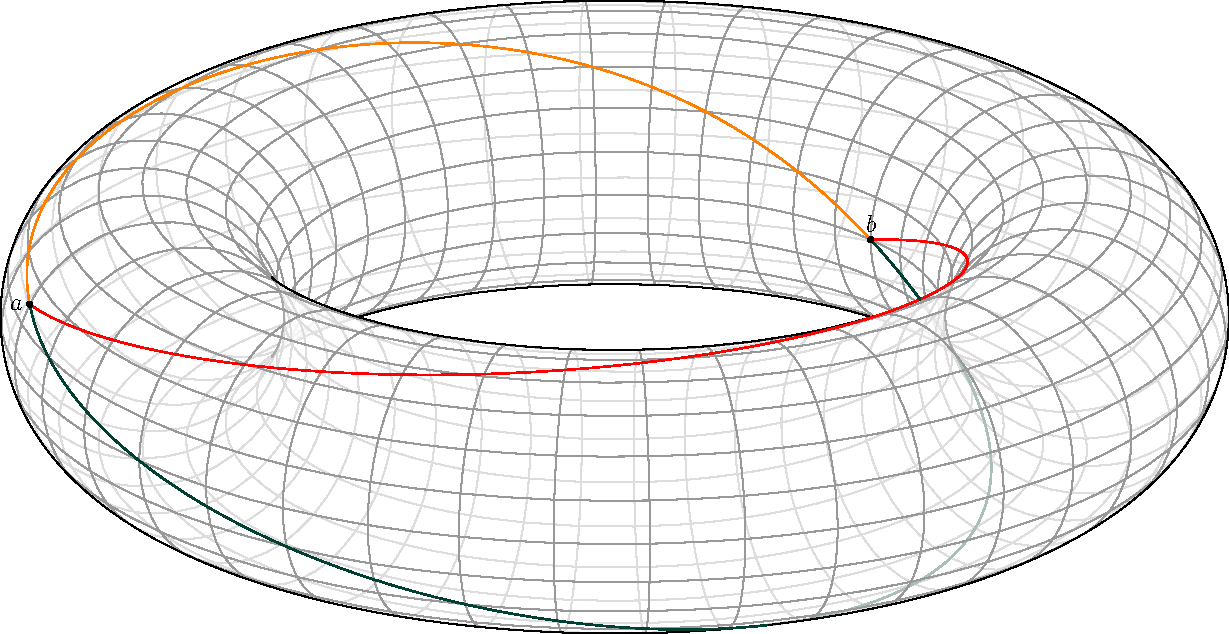
\includegraphics[width=0.45\linewidth, keepaspectratio]{figures/torus-three-paths.pdf}
            \label{fig:torus-three-paths}
        }%
        \label{fig:homotop-paths}
        \caption{Beispiele für (nicht)-Homotopie von Wegen}
    \end{figure}
\end{beispiel}

%%%%%%%%%%%%%%%%%%%%%%%%%%%%%%%%%%%%%%%%%%%%%%%%%%%%%%%%%%%%%%%%%%%%%
% Mitschrieb vom 05.12.2013                                         %
%%%%%%%%%%%%%%%%%%%%%%%%%%%%%%%%%%%%%%%%%%%%%%%%%%%%%%%%%%%%%%%%%%%%%
\begin{bemerkung}\label{kor:homotope-wege}
    Sei $X$ ein topologischer Raum, $\gamma: I \rightarrow X$ ein 
    Weg und $\varphi: I \rightarrow I$ stetig mit $\varphi(0) = 0$,
    $\varphi(1) = 1$. Dann sind $\gamma$ und $\gamma \circ \varphi$
    homotop.
\end{bemerkung}

\begin{beweis}
    Sei $H (t,s) = \gamma ((1-s) t + s \cdot \varphi(t))$.

    Dann ist $H$ stetig, $H(t,0) = \gamma(t),\;\;\; H(t,1) = \gamma ( \varphi(t)),\;\;\;$
    $H(0,s) = \gamma(0)$ und $H(1,s) = \gamma(1-s+s) = \gamma(1)$\\
    $\Rightarrow H$ ist Homotopie. $\qed$
\end{beweis}

\begin{definition}\xindex{Weg!zusammengesetzter}%
    Seien $\gamma_1, \gamma_2$ Wege in $X$ mit $\gamma_1(1) = \gamma_2(0)$.
    Dann ist 
    \[\gamma (t) = \begin{cases}
        \gamma_1(2t)   &\text{falls } 0 \leq t < \frac{1}{2}\\
        \gamma_2(2t-1) &\text{falls } \frac{1}{2} \leq t \leq 1
      \end{cases}\]
    ein Weg in $X$. Er heißt \textbf{zusammengesetzter Weg} und man
    schreibt $\gamma = \gamma_1 * \gamma_2$.
\end{definition}

\begin{bemerkung}\label{kor:assoziativitaet-von-zusammensetzen-von-wegen}
    Das Zusammensetzen von Wegen ist nur bis auf 
    Homotopie assoziativ, d.~h.:
    \begin{align*}
        \gamma_1 * (\gamma_2 * \gamma_3) &\neq (\gamma_1 * \gamma_2) * \gamma_3\\
        \gamma_1 * (\gamma_2 * \gamma_3) &\sim (\gamma_1 * \gamma_2) * \gamma_3
    \end{align*}
    mit $\gamma_1(1)=\gamma_2(0)$ und $\gamma_2(1) = \gamma_3(0)$.
\end{bemerkung}

\begin{beweis}
    \begin{figure}[ht]
        \centering
        \subfloat[$\gamma_1 * (\gamma_2 * \gamma_3)$]{
            \begin{tikzpicture}
    \draw[very thick,red]   (0,0) -- (5,0) node [midway, below] {$\gamma_1$};
    \draw[very thick,green](5,0) -- (7.5,0) node [midway, below] {$\gamma_2$};
    \draw[very thick,blue] (7.5,0) -- (10,0) node [midway, below] {$\gamma_3$};

    \draw[thick] (0,0.2)   -- (  0,-0.2) node[label=below:$0$] {};
    \draw[thick] (5,0.2)   -- (  5,-0.2) node[label=below:$\nicefrac{1}{2}$] {};
    \draw[thick] (7.5,0.2) -- (7.5,-0.2) node[label=below:$\nicefrac{3}{4}$] {};
    \draw[thick] (10,0.2)  -- ( 10,-0.2) node[label=below:$1$] {};
\end{tikzpicture}

            \label{fig:assotiativitaet-von-wegen-a}
        }

        \subfloat[$(\gamma_1 * \gamma_2) * \gamma_3$]{
            \documentclass[varwidth=true, border=2pt]{standalone}
\usepackage{tikz}
\usepackage{nicefrac}

\begin{document}
\begin{tikzpicture}
    \draw[very thick,red]   (0,0) -- (2.5,0) node [midway, below] {$\gamma_1$};
    \draw[very thick,green](2.5,0) -- (5,0) node [midway, below] {$\gamma_2$};
    \draw[very thick,blue] (5,0) -- (10,0) node [midway, below] {$\gamma_3$};

    \draw[thick] (0,0.2)   -- (  0,-0.2) node[label=below:$0$] {};
    \draw[thick] (2.5,0.2) -- (2.5,-0.2) node[label=below:$\nicefrac{1}{4}$] {};
    \draw[thick] (5.0,0.2) -- (5.0,-0.2) node[label=below:$\nicefrac{1}{2}$] {};
    \draw[thick] (10,0.2)  -- ( 10,-0.2) node[label=below:$1$] {};
\end{tikzpicture}
\end{document}

            \label{fig:assotiativitaet-von-wegen-b}
        }%
        \label{fig:assoziativitaet-von-wegen}
        \caption{Das Zusammensetzen von Wegen ist nicht assoziativ}
    \end{figure}

    Das Zusammensetzen von Wegen ist wegen \cref{kor:homotope-wege}
    bis auf Homotopie assoziativ. Verwende dazu

    \[\varphi(t) = \begin{cases}
            \frac{1}{2} t   &\text{falls } 0 \leq t < \frac{1}{2}\\
            t - \frac{1}{4} &\text{falls } \frac{1}{2} \leq t < \frac{3}{4}\\
            2t - 1          &\text{falls } \frac{3}{4} \leq t \leq 1
        \end{cases}\]
\end{beweis}

\begin{bemerkung}\label{kor:bemerkung-10-6}
    Sei $X$ ein topologischer Raum, $a,b,c \in X$, $\gamma_1, \gamma_1'$
    Wege von $a$ nach $b$ und $\gamma_2, \gamma_2'$ Wege von $b$ nach $c$.

    Sind $\gamma_1 \sim \gamma_1'$ und $\gamma_2 \sim \gamma_2'$, so
    ist $\gamma_1 * \gamma_2 \sim \gamma_1 ' * \gamma_2'$.
\end{bemerkung}

\begin{figure}[htp]
    \centering
    \documentclass[varwidth=true, border=2pt]{standalone}

\usepackage{pgfplots}
\usepackage{tikz}

\begin{document}
\begin{tikzpicture}
    \tikzstyle{point}=[circle,thick,draw=black,fill=black,inner sep=0pt,minimum width=4pt,minimum height=4pt]
    \node at (3,1) [red] {$\gamma_1$};
    \node at (1,1) [blue] {$\gamma_1'$};
    \node (a)[point,label=180:$a$] at (0,0) {};
    \node (b)[point,label=-90:$b$]   at (4, 0) {};
    \node (c)[point,label=0:$c$]   at (8, 0) {};
    \draw [rounded corners, thick, red] (a) .. controls (1,-1) .. (2,0)  .. controls (3,1) .. (b);
    \draw [rounded corners, dashed] (a) .. controls (1,-0.8) .. (2,0) .. controls (3,0.8) .. (b);
    \draw [rounded corners, dashed] (a) .. controls (1,-0.6) .. (2,0) .. controls (3,0.6) .. (b);
    \draw [rounded corners, dashed] (a) .. controls (1,-0.4) .. (2,0) .. controls (3,0.4) .. (b);
    \draw [rounded corners, dashed] (a) .. controls (1,-0.2) .. (2,0) .. controls (3,0.2) .. (b);
    \draw [rounded corners, dashed] (a) .. controls (1,   0) .. (2,0) .. controls (3,0.0) .. (b);
    \draw [rounded corners, dashed] (a) .. controls (1, 0.2) .. (2,0) .. controls (3,-0.2) .. (b);
    \draw [rounded corners, dashed] (a) .. controls (1, 0.4) .. (2,0) .. controls (3,-0.4) .. (b);
    \draw [rounded corners, dashed] (a) .. controls (1, 0.6) .. (2,0) .. controls (3,-0.6) .. (b);
    \draw [rounded corners, dashed] (a) .. controls (1, 0.8) .. (2,0) .. controls (3,-0.8) .. (b);
    \draw [rounded corners, dashed] (a) .. controls (1, 1.0) .. (2,0) .. controls (3,-1.0) .. (b);
    \draw [rounded corners, thick, blue] (a) .. controls (1,1) .. (2,0) .. controls (3,-1) .. (b);
    \draw [rounded corners, thick, green!80!black] (b) edge[bend right] node[below] {$\gamma_2'$} (c);
    \draw [rounded corners, dashed] (b) edge[bend right=20] (c);
    \draw [rounded corners, dashed] (b) edge[bend right=-20] (c);
    \draw [rounded corners, dashed] (b) edge[bend right=10] (c);
    \draw [rounded corners, dashed] (b) edge[bend right=-10] (c);
    \draw [rounded corners, thick, orange] (b) edge[bend left] node[above] {$\gamma_1'$} (c);
\end{tikzpicture}
\end{document}

    \caption{Situation aus \cref{kor:bemerkung-10-6}}.
    \label{fig:situation-bemerkung-10-6}
\end{figure}

\begin{beweis}
    Sei $H_i$ eine Homotopie zwischen $\gamma_i$ und $\gamma_i'$,
    $i=1,2$.

    Dann ist 
    \[H(t,s) := \begin{cases}
        H_1(2t, s)  &\text{falls } 0 \leq t \leq \frac{1}{2}\;\;\;\forall s \in I\\
        H_2(2t-1,s) &\text{falls } \frac{1}{2} \leq t \leq 1
    \end{cases}\]

    eine Homotopie zwischen 
    $\gamma_1 * \gamma_2$ und $\gamma_1' * \gamma_2 '$.
\end{beweis}

Eine spezielle Homotopieäquivalenz sind sog. Deformationsretraktionen:
\begin{definition}%
    Sei $X$ ein topologischer Raum, $A \subseteq X$, $r: X \rightarrow A$ eine stetige Abbildung
    und $\iota = (\id_X)|_A$.

    \begin{defenum}
        \item $\iota: A \rightarrow X$ mit $\iota(x) = x$ heißt die 
              \textbf{Inklusionsabbildung}\xindex{Inklusionsabbildung} und
              man schreibt: $\iota: A \hookrightarrow X$.
        \item $r$ heißt \textbf{Retraktion}\xindex{Retraktion}, wenn $r|_A = \id_A$ ist.
        \item $A$ heißt \textbf{Deformationsretrakt}\xindex{Deformationsretrakt}, wenn es eine Retraktion $r$
              auf $A$ mit $\iota  \circ r \sim \id_X$ gibt.
    \end{defenum}
\end{definition}

\begin{beispiel}[Zylinder auf Kreis]
    Sei $X = S^1 \times \mdr$ ein topologischer Raum und
    \[r: S^1 \times \mdr \rightarrow S^1 \times \Set{0} \cong S^1\]
    mit
    \[r(x,y) := (x, 0)\]
    eine Abbildung. $r$ ist eine Retraktion, da $r|_{S^1} \cong \id_{S_1}$.
    \begin{align*}
        \iota \circ r : S^1 \times \mdr &\rightarrow S^1 \times \mdr\\
        (x,y) &\mapsto (x,0)\\
        H: (S^1 \times \mdr) \times I &\rightarrow S^1 \times \mdr\\
        (x, y, t) &\mapsto (x, ty)
    \end{align*}
\end{beispiel}

\section{Fundamentalgruppe}
Für einen Weg $\gamma$ sei $[\gamma]$ seine \textbf{Homotopieklasse}\xindex{Homotopieklasse}.

\begin{definition}\xindex{Fundamentalgruppe}%
    Sei $X$ ein topologischer Raum und $x \in X$. Sei außerdem
    \[\pi_1(X,x) := \Set{[\gamma] | \gamma \text{ ist Weg in } X \text{ mit } \gamma(0) = \gamma(1) = x}\]

    Durch $[\gamma_1] *_G [\gamma_2] : = [\gamma_1 * \gamma_2]$ wird
    $\pi_1(X,x)$ zu einer Gruppe. Diese Gruppe heißt \textbf{Fundamentalgruppe}
    von $X$ im Basispunkt $x$.
\end{definition}

\begin{bemerkung}
    Im $\mdr^2$ gibt es nur eine Homotopieklasse.
\end{bemerkung}

\begin{beweis}[Fundamentalgruppe ist eine Gruppe]\leavevmode
    \begin{enumerate}[label=\alph*)]
        \item Abgeschlossenheit folgt direkt aus der Definition von $*_G$
        \item Assoziativität folgt aus \cref{kor:assoziativitaet-von-zusammensetzen-von-wegen}
        \item Neutrales Element $e = [\gamma_0], \gamma_0(t) = x \;\;\; \forall t \in I$.
              $e * [\gamma] = [\gamma] = [\gamma] * e$, da $\gamma_0 * \gamma \sim \gamma$
        \item \xindex{Weg!inverser} Inverses Element  $[\gamma]^{-1} = [\overline{\gamma}] = [\gamma(1-t)]$, 
              denn $\overline{\gamma} * \gamma \sim \gamma_0 \sim \gamma * \overline{\gamma}$
    \end{enumerate}
\end{beweis}

\begin{beispiel}
    \begin{bspenum}
        \item $S^1 = \Set{z \in \mdc | {|z|} = 1} = \Set{(\cos \varphi, \sin \varphi) \in \mdr^2 | 0 \leq \varphi \leq 2 \pi}$

              $\pi_1 (S^1, 1) = \Set{[\gamma^k] | k \in \mdz} \cong \mdz$.
              Dabei ist $\gamma(t) = e^{2 \pi \iu t} = \cos(2 \pi t) + \iu \sin(2 \pi t)$
              und $\gamma^k := \underbrace{\gamma * \dots * \gamma}_{k \text{ mal}}$

              $[\gamma^k] \mapsto k$ ist ein Isomorphismus.
        \item $\pi_1 (\mdr^2, 0) = \pi_1 (\mdr^2, x) = \Set{e}$ für jedes $x \in \mdr^2$
        \item $\pi_1 (\mdr^n, x) = \Set{e}$ für jedes $x \in \mdr^n$
        \item $G \subseteq \mdr^n$ heißt \textbf{sternförmig}\xindex{sternförmig} bzgl. $x \in G$, 
            wenn für jedes $y \in G$ auch die Strecke $[x, y] \subseteq G$
            ist.

            Für jedes sternförmige $G \subseteq \mdr^n$ ist
            $\pi_1(G,x) = \Set{e}$

            \begin{figure}[htp]
                \centering
                \begin{tikzpicture}[thick]
    \tikzstyle{point}=[circle,thick,draw=black,fill=black,inner sep=0pt,minimum width=4pt,minimum height=4pt]
    \draw[fill=orange!20] (-2,0) -- (-1,0.5) -- (0,2) -- (1,0.5) -- (2,0) -- (1,-0.5) -- (0,-2) -- (-1,-0.5) -- cycle;
    \node (a)[point,label=$x$] at (0,0) {};
\end{tikzpicture}

                \caption{Sternförmiges Gebiet}.
                \label{fig:sternfoermiges-gebiet}
            \end{figure}
        \item $\pi_1(S^2, x_0) = \Set{e}$, da im $\mdr^2$ alle Wege
              homotop zu $\Set{e}$ sind. Mithilfe der stereographischen
              Projektion kann von $S^2$ auf den $\mdr^2$ abgebildet
              werden.

              Dieses Argument funktioniert nicht mehr bei flächenfüllenden
              Wegen, d.~h. wenn $\gamma: I \rightarrow S^2$ surjektiv
              ist.
    \end{bspenum}
\end{beispiel}

\begin{bemerkung}\label{kor:gruppenisomorphismus-wege}
    Sei $X$ ein topologischer Raum, $a,b \in X$, $\delta: I \rightarrow X$
    ein Weg von $a$ nach $b$.

    Dann ist die Abbildung
    \[\alpha: \pi_1 (X, a) \rightarrow \pi_1(X,b)\;\;\;[\gamma] \mapsto [\overline{\delta} * \gamma * \delta]\]
    ein Gruppenisomorphismus.
\end{bemerkung}

\begin{figure}[htp]
    \centering
    \documentclass[varwidth=true, border=2pt]{standalone}

\usepackage{pgfplots}
\usepackage{tikz}

\begin{document}
\begin{tikzpicture}
    \tikzstyle{point}=[circle,thick,draw=black,fill=black,inner sep=0pt,minimum width=4pt,minimum height=4pt]
    \node (a)[point,label=180:$a$] at (0,0) {};
    \node (b)[point,label=0:$b$]   at (3, 0) {};
    \draw [rounded corners,->, thick, red] (a) .. controls (0.5,2) .. (2,1) .. controls (2,0.5) .. (a);
    \draw [rounded corners,->, thick, blue] (a) .. controls (1,-1) .. (2,-0.5) .. controls (2.2,-1) .. (b);
    \node at (1,1.2) [red] {$\gamma$};
\end{tikzpicture}
\end{document}

    \caption{Situation aus \cref{kor:gruppenisomorphismus-wege}}.
    \label{fig:situation-gruppenisomorphismus-wege}
\end{figure}

\begin{beweis}
    \begin{align*}
        \alpha([\gamma_1] * [\gamma_2]) &= [\overline{\delta} * (\gamma_1 * \gamma_2) * \delta]\\
        &= [\overline{\delta} * \gamma_1 * \delta * \overline{\delta} * \gamma_2 * \delta]\\
        &= [\overline{\delta} * \gamma_1 * \delta] * [\overline{\delta} * \gamma_2 * \delta]\\
        &= \alpha([\gamma_1]) * \alpha([\gamma_2])
    \end{align*}
\end{beweis}

%%%%%%%%%%%%%%%%%%%%%%%%%%%%%%%%%%%%%%%%%%%%%%%%%%%%%%%%%%%%%%%%%%%%%
% Tânias Mitschrieb vom 10.12.2013                                  %
%%%%%%%%%%%%%%%%%%%%%%%%%%%%%%%%%%%%%%%%%%%%%%%%%%%%%%%%%%%%%%%%%%%%%
\begin{definition}\xindex{einfach zusammenhängend}%11.4
    Ein wegzusammenhängender topologischer Raum $X$ heißt
    \textbf{einfach zusammenhängend}, wenn $\pi_1(X,x) = \Set{e}$
    für ein $x \in X$.
\end{definition}

Wenn $\pi_1(X,x) = \Set{e}$ für ein $x \in X$ gilt, dann wegen 
\cref{kor:gruppenisomorphismus-wege} sogar für alle $x \in X$.

\begin{bemerkung}\label{korr:11.5}
    Es seien $X, Y$ topologische Räume, $f:X \rightarrow Y$ eine
    stetige Abbildung, $x \in X, y := f(x) \in Y$.

    \begin{bemenum}
        \item Dann ist die Abbildung $f_* : \pi_1(X,x) \rightarrow \pi_1(Y, y),
        [\gamma] \rightarrow [f \circ \gamma]$ ein Gruppenhomomorphismus.
        \item Ist $Z$ ein weiterer topologischer Raum und $g: Y \rightarrow Z$
              eine stetige Abbildung $z:= g(y)$. Dann ist
              $(g \circ f)_* = g_* \circ f_*: \pi_1(X,x) \rightarrow \pi_1(Z,z)$
    \end{bemenum}
\end{bemerkung}

\begin{beweis}\leavevmode
    \begin{enumerate}[label=\alph*)]
        \item $f_*$ ist wohldefiniert: Seien $\gamma_1, \gamma_2$ homotope
              Wege von $x$. z.Z.: $f \circ \gamma_1 \sim f \circ \gamma_2$:
              Nach Voraussetzung gibt es stetige Abbildungen $H:I\times I \rightarrow X$
              mit 
              \begin{align*}
                H(t,0) &= \gamma_1(t),\\
                H(t,1) &= \gamma_2(t),\\
                H(0,s) &= H(1, s) = x\text{.}
              \end{align*}
              Dann ist $f \circ H: I \times I \rightarrow Y$ stetig mit
              $(f \circ H)(t,0) = f(H(t,0)) = f(\gamma_1(t)) = (f \circ \gamma_1)(t)$
              etc. $\Rightarrow f \circ \gamma_1 \sim f \circ \gamma_2$.

              $f_*([\gamma_1] * [\gamma_2]) = [f \circ (\gamma_1 * \gamma_2)] = [(f \circ \gamma_1)] * [(f \circ \gamma_2)] = f_*([\gamma_1]) * f_*([\gamma_2])$
        \item $(g \circ f)_* ([\gamma]) = [(g \circ f) \circ \gamma] = [g \circ (f \circ \gamma)] = g_* ([f \circ \gamma]) = g_* (f_* ([\gamma])) = (g_* \circ f_*)([\gamma])$
    \end{enumerate}
\end{beweis}

\begin{beispiel}
    \begin{bspenum}
        \item $f:S^1 \hookrightarrow \mdr^2$ ist injektiv, aber 
              $f_*:\pi_1(S^1, 1) \cong \mdz \rightarrow \pi_1(\mdr^2, 1) = \Set{e}$
              ist nicht injektiv.
        \item $f: \mdr \rightarrow S^1, t \mapsto (\cos 2 \pi t, \sin 2 \pi t)$
              ist surjektiv, aber $f_*: \pi_1(\mdr, 0) = \Set{e} \rightarrow \pi_1(S^1, 1) \cong \mdz$
              ist nicht surjektiv.
    \end{bspenum}
\end{beispiel}

\begin{bemerkung}%Folgerung 11.6
    Sei $f:X \rightarrow Y$ ein Homöomorphismus zwischen topologischen
    Räumen $X, Y$. Dann gilt:

    \[f_*: \pi_1(X,x) \rightarrow \pi_1(Y, f(x))\]
    ist ein Isomorphismus für jedes $x \in X$.
\end{bemerkung}

\begin{beweis}
    Sei $g: Y \rightarrow X$ die Umkehrabbildung, d.~h. $g$ ist stetig
    und $f \circ g = \id_Y$, $g \circ f = \id_X$

    $\Rightarrow f_* \circ g_* = (f \circ g)_* = (\id_Y)_* = \id_{\pi_1 (Y, f(X)}$
    und $g_* \circ f_* = \id_{\pi_1(X,x)}$.
\end{beweis}

\begin{definition}\xindex{Abbildung!homotope}%
    Seien $X, Y$ topologische Räume, $x_0 \in X, y_0 \in Y, f, g: X \rightarrow Y$
    stetig mit $f(x_0) = y_0 = g(x_0)$.

    $f$ und $g$ heißen \textbf{homotop} ($f \sim g$), wenn es eine stetige
    Abbildung $H: X \times I \rightarrow Y$ mit 
    \begin{align*}
        H(x,0)    &= f(x) \; \forall x \in X\\
        H(x,1)    &= g(x) \; \forall x \in X\\
        H(x_0, s) &= y_0  \; \forall s \in I
    \end{align*}
    gibt.
\end{definition}

\begin{bemerkung}
    Sind $f$ und $g$ homotop, so ist $f_* = g_*: \pi_1 (X, x_0) \rightarrow \pi_1(Y, y_0)$.
\end{bemerkung}

\begin{beweis}
    Sei $\gamma$ ein geschlossener Weg in $X$ um $x_0$, d.~h.
    $[\gamma] \in \pi_1 (X, x_0)$.

    Z.~z.: $f \circ \gamma \sim g \circ \gamma$

    Sei dazu $H_\gamma: I \times I \rightarrow Y, (t,s) \mapsto H(\gamma(t), s)$.
    Dann gilt: 
        \begin{align*}
            H_\gamma(t,0) &= H(\gamma(t), 0) = (f \circ \gamma)(t) \;\forall t \in I\\
            H_\gamma(1,s) &= H(\gamma(1), s) = H(x_0, s) = y_0\;\forall s \in I\\
            H_\gamma(t,1) &= H(\gamma(t), 1) = g(\gamma(t))\;\forall t \in I
        \end{align*}
\end{beweis}

\begin{beispiel}
    $f:X \rightarrow Y, g: Y \rightarrow X$ mit $g \circ f \sim \id_X,$
    $f \circ g \sim \id_Y$

    $\Rightarrow f_*$ ist Isomorphismus. Konkret: $f: \mdr^2 \rightarrow \Set{0},$
    $g:\Set{0} \rightarrow \mdr^2$

    $\Rightarrow f \circ g = \id_{\Set{0}}$, $g \circ f: \mdr^2 \rightarrow \mdr^2$,
    $x \mapsto 0$ für alle $x$.

    $g \circ f \sim \id_{\mdr^2}$ mit Homotopie: $H: \mdr^2 \times I \rightarrow \mdr^2, H(x,s) = (1-s) x$ (stetig!)

    $\Rightarrow H(x,0) = x = \id_{\mdr^2} (x)$, $H(x, 1) = 0$, $H(0, s) = 0\;\forall s \in I$.
\end{beispiel}

\begin{satz}[Satz von Seifert und van Kampen \enquote{light}]\label{thm:seifert-van-kampen}
    Sei $X$ ein topologischer Raum, $U, V \subseteq X$ offen mit 
    $U \cup V = X$ und $U \cap V$ wegzusammenhängend.

    Dann wird $\pi_1(X,x)$ für $x \in U \cap V$ erzeugt von geschlossenen
    Wegen um $x$, die ganz in $U$ oder ganz in $V$ verlaufen.
\end{satz}

\begin{beweis}
    Sei $\gamma: I \rightarrow X$ ein geschlossener Weg um $x$.
    Überdecke $I$ mit endlich vielen offenen Intervallen
    $I_1, I_2, \dots, I_n$, die ganz in 
    $\gamma^{-1}(U)$ oder ganz in $\gamma^{-1}(V)$ liegen.

    \Obda sei $\gamma(I_1) \subseteq U, \gamma(I_2) \subseteq V$, etc.

    Wähle $t_i \in I_i \cap I_{i+1}$, also $\gamma(t_i) \in U \cap V$.
    Sei $\sigma_i$ Weg in $U \cap V$ von $x_0$ nach $\gamma(t_i) \Rightarrow \gamma$
    ist homotop zu 
    \[\underbrace{\gamma_1 * \overline{\sigma_1}}_{\text{in } U} * \underbrace{\sigma_1 * \gamma_2 * \overline{\sigma_2}}_{\text{in } V} * \dots * \sigma_{n-1} * \gamma_2 \text{ mit } \gamma_i := \gamma |_{I_i}\]
\end{beweis}

\begin{beispiel}[Satz von Seifert und van Kampen]
    \begin{bspenum}
        \item
            \begin{figure}[htp]
                \centering
                \begin{tikzpicture}[thick]
    \tikzstyle{point}=[circle,thick,draw=black,fill=black,inner sep=0pt,minimum width=4pt,minimum height=4pt]
    \node[blue]   at (4.5, 1.7) {$a$};
    \node[purple] at (7.5, 1.7) {$b$};
    \begin{scope}[xshift=5cm, yshift=1cm]
        \draw[blue,->]   (  0,0)+(150:0.7cm) arc (150:510:0.7cm);
        \draw[purple,<-] (1.4,0)+( 40:0.7cm) arc (40:400:0.7cm);
        \node (z)[point,label={[label distance=0.2cm]-90:$x$}] at (0.7,0) {};
    \end{scope}
\end{tikzpicture}

                \caption{Topologischer Raum $X$}
                \label{fig:top-raum-kreise}
            \end{figure}

            Sei $X$ wie in \cref{fig:top-raum-kreise}. $\pi_1(X,x)$ wird \enquote{frei} erzeugt von $a$ und $b$, weil
            $\pi_1(U,x) = \langle a \rangle \cong \mdz, \pi_1(V,x) = \langle b \rangle \cong \mdz$,
            insbesondere ist $a*b$ nicht homotop zu $b*a$.
        \item Torus\xindex{Torus}: $\pi_1(T^2, X)$ wird erzeugt von $a$ und $b$.
            \begin{figure}[htp]
                \centering
                \documentclass[varwidth=true, border=2pt]{standalone}
\usepackage{tikz}
\usetikzlibrary{patterns}

\begin{document}
\begin{tikzpicture}[thick]
    \draw[pattern=north east lines] (-3,3) -- (3,3) -- (3,-3) -- (-3,-3) -- cycle;
    \draw[red, pattern color=red, pattern=north west lines] (-3,-1) -- (-1,-1) -- (-1,-3) -- (-3,-3) -- cycle;
    \draw[red, pattern color=red, pattern=north west lines] (-3,3) -- (-1,3) -- (-1,1) -- (-3,1) -- cycle;
    \draw[red, pattern color=red, pattern=north west lines] (1,3) -- (3,3) -- (3,1) -- (1,1) -- cycle;
    \draw[red, pattern color=red, pattern=north west lines] (1,-1) -- (3,-1) -- (3,-3) -- (1,-3) -- cycle;
    \draw[->,blue] (-3,-1.5) -- (-2,-1.5);
    \draw[blue] (-2,-1.5) -- (-1.5,-1.5);
    \draw[->,blue] (-1.5,-1.5) -- (-1.5,-2.3);
    \draw[blue] (-1.5, -2.3) -- (-1.5, -3);
    \draw[green] (-3,-2) -- (-2,-2) -- (-2, -3);
\end{tikzpicture}
\end{document}

                \caption{$a*b = b*a \Leftrightarrow a * b * \overline{a} * \overline{b} \sim e$}
                \label{fig:torous-a-b}
            \end{figure}
    \end{bspenum}
\end{beispiel}

%%%%%%%%%%%%%%%%%%%%%%%%%%%%%%%%%%%%%%%%%%%%%%%%%%%%%%%%%%%%%%%%%%%%%
% Mitschrieb vom 12.12.2013                                         %
%%%%%%%%%%%%%%%%%%%%%%%%%%%%%%%%%%%%%%%%%%%%%%%%%%%%%%%%%%%%%%%%%%%%%
\section{Überlagerungen}\index{Ueberlagerung@""Uberlagerung|(}
\begin{figure}[htp]
    \centering
    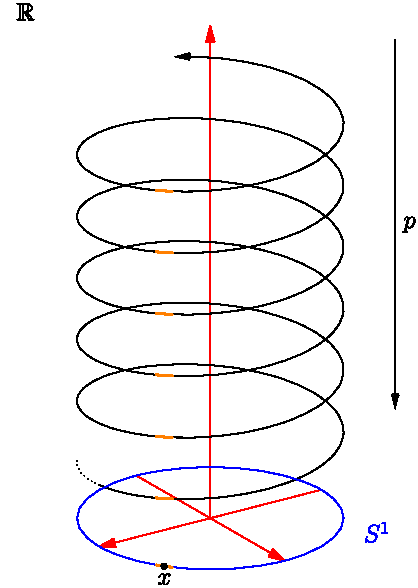
\includegraphics[width=4cm, keepaspectratio]{figures/topology-r-spiral-covering-s.pdf}
    \caption{$\mdr \rightarrow S^1$,\\$t \mapsto (\cos 2 \pi t, \sin 2 \pi t)$}
    \label{fig:ueberlappung-r1-spirale-s1}
\end{figure}
\begin{definition}\xindex{Ueberlagerung@""Uberlagerung}\label{def:12.1}%Definition 12.1 der Vorlesung
    Es seien $X, Y$ zusammenhängende topologische Räume und
    $p: Y \rightarrow X$ eine stetige Abbildung.

    $p$ heißt \textbf{Überlagerung}, wenn jedes $x \in X$ eine offene
    Umgebung $U = U(x) \subseteq X$ besitzt, sodass $p^{-1}(U)$ disjunkte Vereinigung
    von offenen Teilmengen $V_j \subseteq Y$ ist $(j \in I)$ und
    $p|_{V_j}: V_j \rightarrow U$ ein Homöomorphismus ist.
\end{definition}

\begin{beispiel}
    \begin{bspenum}
        \item siehe \cref{fig:ueberlappung-r1-spirale-s1}
        \item siehe \cref{fig:ueberlappung-kaestchen-torus}
        \item $\mdr^n \rightarrow T^n = \mdr^n / \mdz^n$
        \item $S^n \rightarrow \praum^n(\mdr)$\xindex{Raum!projektiver}
        \item $S^1 \rightarrow S^1$, $z \mapsto z^2$, siehe \cref{fig:liftung-s1-s1}
    \end{bspenum}

    \begin{figure}[htp]
        \centering
        \resizebox{0.95\linewidth}{!}{% The following answers were used to create this image:
% - http://tex.stackexchange.com/a/45824/5645 - Grid
% - http://tex.stackexchange.com/a/373/5645 - Torus
\documentclass[border=2pt]{standalone}
\usepackage{amsmath,amssymb}
\usepackage{tikz}
\usetikzlibrary{patterns,arrows,positioning}

\begin{document}
\begin{tikzpicture}
\tikzstyle{point}=[circle,thick,draw=black,fill=black,inner sep=0pt,minimum width=4pt,minimum height=4pt]
\newcommand*{\xMin}{0}%
\newcommand*{\xMax}{6}%
\newcommand*{\yMin}{0}%
\newcommand*{\yMax}{6}%

\draw (-3.5,0) .. controls (-3.5,2) and (-1.5,2.5) .. (0,2.5);
\draw[xscale=-1] (-3.5,0) .. controls (-3.5,2) and (-1.5,2.5) .. (0,2.5);
\draw[rotate=180] (-3.5,0) .. controls (-3.5,2) and (-1.5,2.5) .. (0,2.5);
\draw[yscale=-1] (-3.5,0) .. controls (-3.5,2) and (-1.5,2.5) .. (0,2.5);

\draw (-2,.2) .. controls (-1.5,-0.3) and (-1,-0.5) .. (0,-.5) .. controls (1,-0.5) and (1.5,-0.3) .. (2,0.2);
\draw (-1.75,0) .. controls (-1.5,0.3) and (-1,0.5) .. (0,.5) .. controls (1,0.5) and (1.5,0.3) .. (1.75,0);


\begin{scope}[shift={(-12,-3)}]
    \foreach \i in {\xMin,...,\xMax} {
        \draw [very thin,gray] (\i,\yMin) -- (\i,\yMax)  node [below] at (\i,\yMin) {$\i$};
    }
    \foreach \i in {\yMin,...,\yMax} {
        \draw [very thin,gray] (\xMin,\i) -- (\xMax,\i) node [left] at (\xMin,\i) {$\i$};
    }

    \begin{scope}[shift={(14,2)}]
        \node (P) at (0.4,0.9) {};
        \node (Q) at (0.9,0.4) {};
        \draw [red] (P) rectangle (Q);
        \draw (0.65, 0.6) node[red] {*};
    \end{scope}

    \foreach \x in {0,1,2,3,4,5} {
        \foreach \y in {0,1,2,3,4,5} {
            \begin{scope}[shift={(\x,\y)}]
                \node (P) at (0.4,0.9) {};
                \node (Q) at (0.9,0.4) {};
                \draw [red] (P) rectangle (Q);
                \draw (0.65, 0.6) node[red] {*};
            \end{scope}
        }
    }
\end{scope}
    \draw (-4.5, 0) node[below] {$\xrightarrow{\text{\;\;\;\;\;\;\;\;}}$};
\end{tikzpicture}
\end{document}
}
        \caption{$\mdr^2 \rightarrow T^2 = \mdr^2 / \mdz^2$}
        \label{fig:ueberlappung-kaestchen-torus}
    \end{figure}
    \begin{figure}[htp]
        \centering
        \newcommand\markangle[6]{% origin X Y radius radiusmark mark
  % fill red circle
  \begin{scope}
    \path[clip] (#1) -- (#2) -- (#3);
    \fill[color=red,fill opacity=0.5,draw=red,name path=circle]
    (#1) circle (#4);
  \end{scope}
  % middle calculation
  \path[name path=line one] (#1) -- (#2);
  \path[name path=line two] (#1) -- (#3);
  \path[%
  name intersections={of=line one and circle, by={inter one}},
  name intersections={of=line two and circle, by={inter two}}
  ] (inter one) -- (inter two) coordinate[pos=.5] (middle);
  % put mark
  \node at ($(#1)!#5!(middle)$) {#6};
}

\begin{tikzpicture}
    \newcommand{\R}{2}
    \draw (0,0) circle (\R);
    \draw[->, thick] ({-(\R+0.2)},0) -- ({\R+0.2},0);
    \draw[->, thick] (0,{-(\R+0.2)}) -- (0,{\R+0.2});
    \draw[thick] (\R,-0.06) -- (\R,0.06) node[label=below:$1$] {};
    \draw[thick] (-0.06,\R) -- (0.06,\R) node[label=left:$i$] {};
    \draw (0,0) -- ({\R*cos(30)},{\R*sin(30)}) node[label=15:$z$] {};
    \draw (0,0) -- ({\R*cos(60)},{\R*sin(60)}) node[label=35:$z^2$] {};

    \coordinate (O) at (0,0);
    \coordinate (X) at (1,0);
    \coordinate (Y) at ({\R*cos(30)},{\R*sin(30)});
    \coordinate (Z) at ({\R*cos(60)},{\R*sin(60)});
    \markangle{O}{Y}{Z}{10mm}{7mm}{$\varphi$}
    \markangle{O}{X}{Y}{10mm}{7mm}{$\varphi$}

    \begin{scope}[xshift=4cm, yshift=-1.2cm]
        \draw (0,0) circle (\R/2);
        \newcommand{\x}{1}
        \draw [red,thick,domain=-30:30] plot ({cos(\x)}, {sin(\x)});
        \draw [red,thick,domain=210:150] plot ({cos(\x)}, {sin(\x)});
    \end{scope}

    \begin{scope}[xshift=4cm, yshift=+1.2cm]
        \draw (0,0) circle (\R/2);
        \newcommand{\x}{1}
        \draw [red,thick,domain=-30:30] plot ({cos(\x)}, {sin(\x)});
    \end{scope}

    \coordinate (T) at (5.5,1);
    \path[->] (5.5,-1) edge[bend right] node[label=right:$z^2$] {} (T);
\end{tikzpicture}

        \caption{$t \mapsto (\cos 4 \pi t, \sin 4 \pi t)$}
        \label{fig:liftung-s1-s1}
    \end{figure}
\end{beispiel}

\begin{bemerkung}
    Überlagerungen sind surjektiv.
\end{bemerkung}

\begin{beweis}
    Sei $p: Y \rightarrow X$ eine Überlagerung und $x \in X$ beliebig.
    Dann existiert eine offene Umgebung $U(x) \subseteq X$ und offene
    Teilmengen $V_j \subseteq X$ mit 
    $p^{-1}(U) = \Dcup V_j$ und
    $p|_{V_j}: V_j \rightarrow U$ ist Homöomorphismus.

    D.~h. es existiert ein $y \in V_j$, so dass $p|_{V_j}(y) = x$.
    Da $x \in X$ beliebig war und ein $y \in Y$ existiert, mit 
    $p(y) = x$, ist $p$ surjektiv.    $\qed$
\end{beweis}

\begin{definition}\xindex{Abbildung!offene}%
    Seien $(X, \fT_X), (Y, \fT_Y)$ topologische Räume und $f:X \rightarrow Y$ eine 
    Abbildung.

    $f$ heißt \textbf{offen} $:\gdw \forall U \in \fT_X: f(U) \in \fT_Y$.
\end{definition}

\begin{beispiel}[Offene und stetige Abbildungen]
    Sei $X$ ein topologischer Raum und seien
    $f_i: \mdr \rightarrow \mdr$ mit $i \in \Set{1,2,3}$ und
    $g: \mdr \rightarrow S^1 = \Set{z \in \mdc | \|z\| = 1}$ Abbildungen.
    \begin{bspenum}
        \item $f_1 := \id_\mdr$ ist eine offene und stetige Abbildung.
        \item $g(x) := e^{2 \pi \iu x}$ ist eine offene, aber keine stetige Abbildung (vgl. \cref{fig:nicht-stetige-umkehrabbildung}).
        \item $f_2(x) := 42$ ist eine stetige, aber keine offene Abbildung.
        \item $f_3(x) := \begin{cases}
                0  &\text{falls } x \in \mdq\\
                42 &\text{falls } x \in \mdr \setminus \mdq
        \end{cases}$\\
        ist weder stetig noch offen.
    \end{bspenum}
\end{beispiel}

\begin{bemerkung}\label{bem:12.2} % Bemerkung 12.2 der Vorlesung
    Überlagerungen sind offene Abbildungen.
\end{bemerkung}

\begin{beweis}
    Sei $y \in V$ und $x \in p(V)$, sodass $x=p(y)$ gilt.
    Sei weiter $U = U_x$ eine offene Umgebung von $x$ wie in \cref{def:12.1}
    und $V_j$ die Komponente von $p^{-1}(U)$, die $y$ enthält.

    Dann ist $V \cap V_j$ offene Umgebung von $y$.

    $\Rightarrow p(V \cap V_j)$ ist offen in $p(V_j)$, also auch offen
    in $X$. Außerdem ist $p(y) = x \in p(V \cap V_j)$ und
    $p(V \cap V_j) \subseteq p(V)$.

    $\Rightarrow p(V)$ ist offen.
\end{beweis}

\begin{definition}\xindex{diskret}%
    Sei $X$ ein topologischer Raum und $M \subseteq X$.

    $M$ heißt \textbf{diskret} in $X$, wenn $M$ in $X$ keinen 
    Häufungspunkt hat.
\end{definition}

\begin{bemerkung} % Bemerkung 12.3 der Vorlesung
    Sei $p: Y \rightarrow X$ Überlagerung, $x \in X$.
    \begin{bemenum}
        \item $X$ hausdorffsch $\Rightarrow Y$ hausdorffsch
        \item $p^{-1}(x)$ ist diskret in $Y$ für jedes $x \in X$.
    \end{bemenum}
\end{bemerkung}

\begin{beweis}\leavevmode
    \begin{enumerate}[label=\alph*)]
        \item Seien $y_1, y_2 \in Y$.

        \underline{1. Fall}: $p(y_1) = p(y_2) = x$.

        Sei $U$ Umgebung von $x$ wie in \cref{def:12.1},
        $V_{j_1}$ bzw. $V_{j_2}$ die Komponente von $p^{-1}(U)$, die
        $y_1$ bzw. $y_2$ enthält.

        Dann ist $V_{j_1} \neq V_{j_2}$, weil beide ein Element aus $p^{-1}(x)$
        enthalten.

        $\Rightarrow V_{j_1} \cap V_{j_2} = \emptyset$ nach Voraussetzung.

        \underline{2. Fall}: $p(y_1) \neq p(y_2)$.
        
        Dann seien $U_1$ und $U_2$ disjunkte Umgebungen von $p(y_1)$
        und $p(y_2)$.

        $\Rightarrow p^{-1}(U_1)$ und $p^{-1}(U_2)$ sind disjunkte 
        Umgebungen von $y_1$ und $y_2$.

        \item Sei $x \in X$ beliebig, aber fest.

        \underline{Zu zeigen}: $\forall y_i \in p^{-1}(x): \exists V_i \in \fT_Y \text{ mit } y_i \in V_i \text{, sodass gilt:} i \neq j \Rightarrow V_i \cap V_j = \emptyset$.

        Die $V_i$ existieren wegen der Definition einer Überlagerung:
        $p$ heißt Überlagerung $:\gdw \forall x \in X \exists U=U(x) \in \fT_X: p^{-1}(U) = \Dcup_{V_i \in \fT_Y} V_i \text{ und } p|_{V_i} \text{ ist Homöomorphismus}$.\\
        $\Rightarrow (p|_{V_i})^{-1}(x) = \Set{y_i}$\\
        $\Rightarrow$ Alle $y_i$ liegen diskret in $Y$, da Häufungspunkte unendlich
        viele Elemente in jeder Umgebung benötigen. $\qed$
    \end{enumerate}
\end{beweis}

\begin{bemerkung}\label{kor:12.4}%Bemerkung 12.4 der Vorlesung
    Sei $p: Y \rightarrow X$ Überlagerung, $x_1, x_2 \in X$.

    Dann ist $|p^{-1} (x_1)| = |p^{-1}(x_2)|$.\footnote{$|p^{-1} (x_1)| = \infty$ ist erlaubt!}
\end{bemerkung}

\begin{beweis}
    Sei $U$ Umgebung von $x_1$ wie in \cref{def:12.1}, $x \in U$.
    Dann enthält jedes $V_j, j \in I_X$ genau ein Element von
    $p^{-1}(x)$

    $\Rightarrow |p^{-1} (x)|$ ist konstant auf $U$

    $\xRightarrow{X \text{zhgd.}} |p^{-1}(x)|$  ist konstant auf $X$
\end{beweis}

\begin{definition}\xindex{Liftung}%
    Es seien $X, Y, Z$ topologische Räume,
    $p: Y \rightarrow X$ eine Überlagerung und $f:Z \rightarrow X$ stetig.

    Eine stetige Abbildung $\tilde{f}: Z \rightarrow Y$ heißt
    \textbf{Liftung} von $f$, wenn $p \circ \tilde{f} = f$ ist.
\end{definition}

\begin{figure}[h]
    \centering
    \begin{tikzpicture}
      \node (Y) {$Y$};
      \node (X) [below=0.7cm of Y] {$X$};
      \node (Z) [right=1.3cm of Y] {$Z$};
      \path[anchor=east,->] (Y) edge node {$p$} (X);
      \path[anchor=south,->] (Z) edge node {$\tilde{f}$} (Y);
      \path[anchor=north west,->] (Z) edge node {$f$} (X);
    \end{tikzpicture}
\end{figure}

\begin{figure}[htp]
    \centering
    \resizebox{0.95\linewidth}{!}{% The following answers were used to create this image:
% - http://tex.stackexchange.com/a/45824/5645 - Grid
% - http://tex.stackexchange.com/a/373/5645 - Torus
\begin{tikzpicture}
\tikzstyle{point}=[circle,thick,draw=black,fill=black,inner sep=0pt,minimum width=4pt,minimum height=4pt]
\newcommand*{\xMin}{0}%
\newcommand*{\xMax}{6}%
\newcommand*{\yMin}{0}%
\newcommand*{\yMax}{6}%

\draw (-3.5,0) .. controls (-3.5,2) and (-1.5,2.5) .. (0,2.5);
\draw[xscale=-1] (-3.5,0) .. controls (-3.5,2) and (-1.5,2.5) .. (0,2.5);
\draw[rotate=180] (-3.5,0) .. controls (-3.5,2) and (-1.5,2.5) .. (0,2.5);
\draw[yscale=-1] (-3.5,0) .. controls (-3.5,2) and (-1.5,2.5) .. (0,2.5);

\draw (-2,.2) .. controls (-1.5,-0.3) and (-1,-0.5) .. (0,-.5) .. controls (1,-0.5) and (1.5,-0.3) .. (2,0.2);

\draw (-1.75,0) .. controls (-1.5,0.3) and (-1,0.5) .. (0,.5) .. controls (1,0.5) and (1.5,0.3) .. (1.75,0);

\begin{scope}[shift={(5,-3)}]
    \foreach \i in {\xMin,...,\xMax} {
        \draw [very thin,gray] (\i,\yMin) -- (\i,\yMax)  node [below] at (\i,\yMin) {$\i$};
    }
    \foreach \i in {\yMin,...,\yMax} {
        \draw [very thin,gray] (\xMin,\i) -- (\xMax,\i) node [left] at (\xMin,\i) {$\i$};
    }

    \node (P)[point,red] at (1.2,2.2) {};
    \node (Q)[point,red] at (1.2,1.6) {};
    \draw[ultra thick, red] (P) -- (Q);

    \begin{scope}[shift={(2,1)}]
        \node (P)[point,red] at (1.2,2.2) {};
        \node (Q)[point,red] at (1.2,1.6) {};
        \draw[ultra thick, red] (P) -- (Q);
    \end{scope}
    \draw (-1, -0.5) node[below] {$T \xrightarrow{\text{Liften}} \mathbb{R}^2 / \mathbb{Z}^2$};
    \draw[red,dashed] (-5,1.5) ellipse (0.5cm and 1cm);

    \draw[red] (-5,2.5) arc (-270:-90:0.5 and 1) ;
\end{scope}
\end{tikzpicture}
}
    \caption{Beim Liften eines Weges bleiben geschlossene Wege im allgemeinen nicht geschlossen}
    \label{fig:satz-seifert-van-kampen}
\end{figure}

\begin{bemerkung}[Eindeutigkeit der Liftung]\label{kor:12.5}%Bemerkung 12.5 aus Vorlesung
    Sei $Z$ zusammenhängend und $f_0, f_1: Z \rightarrow Y$
    Liftungen von $f$.

    $\exists z_0 \in Z: f_0(z_0) = f_1(z_0) \Rightarrow f_0 = f_1$
\end{bemerkung}

% \begin{figure}[htp]
%     \centering
%     \documentclass{article}
\usepackage[pdftex,active,tightpage]{preview}
\setlength\PreviewBorder{2mm}
\usepackage{tikz}

\begin{document}
\begin{preview}
\begin{tikzpicture}
    \node (Z) at (0,0) {$Z$};
    \node (Y) at (3,0) {$Y$};
    \node (X) at (1.5,-1.5) {$X$};
    \draw[->, above, dashed] (Z) to node {$\tilde{f}$} (Y);
    \draw[->, below] (Z)  to node {$f$} (X);
    \draw[->, right] (Y)  to node {$p$} (X);

    \begin{scope}[xshift=1.3cm,yshift=-0.6cm]
        \draw (0,0) -- (0.3,0.3);
        \draw (0.1,0) -- (0.4,0.3);
        \draw (0.2,0) -- (0.5,0.3);
    \end{scope}
\end{tikzpicture}
\end{preview}
\end{document}

%     \caption{Situation aus \cref{kor:12.5}}
%     \label{fig:situation-kor-12.5}
% \end{figure}

\begin{beweis}
    Sei $T = \Set{z \in Z | f_0(z) = f_1(z)}$.

    \underline{Z.~z.}: $T$ ist offen und $Z \setminus T$ ist auch offen.

    Sei $z \in T, x = f(z), U$ Umgebung von $x$ wie in \cref{def:12.1},
    $V$ die Komponente von $p^{-1}(U)$, die $y:=f_0(z) = f_1(z)$
    enthält.

    Sei $q:U \rightarrow V$ die Umkehrabbildung zu $p|_V$.

    Sei $W:= f^{-1}(U) \cap f_0^{-1}(V) \cap f_1^{-1}(V)$. $W$ ist 
    offene Umgebung in $Z$ von $z$.

    \underline{Behauptung:} $W \subseteq T$

    Denn für $w \in W$ ist $q(f(w)) = q((p \circ f_0))(w) = ((q \circ p) \circ f_0) (w) = f_0(w) = q(f(w)) = f_1(w)$

    $\Rightarrow T$ ist offen.

    Analog: $Z \setminus T$ ist offen.
\end{beweis}

\begin{satz}\label{thm:ueberlagerung-weg-satz-12.6}
    Sei $p: Y \rightarrow X$ Überlagerung, $\gamma: I \rightarrow X$
    ein Weg, $y \in Y$ mit $p(y) = \gamma(0) =: x$.

    Dann gibt es genau einen Weg $\tilde{\gamma}: I \rightarrow Y$
    mit $\tilde{\gamma}(0)=y$ und $p \circ \tilde{\gamma} = \gamma$.
\end{satz}

%%%%%%%%%%%%%%%%%%%%%%%%%%%%%%%%%%%%%%%%%%%%%%%%%%%%%%%%%%%%%%%%%%%%%
% Sebastians Mitschrieb vom 17.12.2013                              %
%%%%%%%%%%%%%%%%%%%%%%%%%%%%%%%%%%%%%%%%%%%%%%%%%%%%%%%%%%%%%%%%%%%%%
$p:Y \rightarrow X$ Überlagerung, $X,Y$ wegzusammenhängend.
$p$ stetig und surjektiv, zu $x \in X \exists$ Umgebung $U$, so dass
$p^{-1}(U) = \bigcup V_j$

$p|_{V_j}: V_j \rightarrow U$ Homöomorphismus.

\begin{bemerkung}%Bemerkung 12.6 der Vorlesung
    Wege in $X$ lassen sich zu Wegen in $Y$ liften.

    Zu jedem $y \in p^{-1}(\gamma(0))$ gibt es genau einen Lift von 
    $\gamma$.
\end{bemerkung}

\begin{proposition}\label{proposition:12.7}%Proposition 12.7 der Vorlesung
    Seien $p: Y \rightarrow X$ eine Überlagerung, $a,b \in X$,
    $\gamma_0, \gamma_1: I \rightarrow X$ homotope Wege von $a$ nach
    $b$, $\tilde{a} \in p^{-1}(a), \tilde{\gamma_0}, \tilde{\gamma_1}$
    Liftungen von $\gamma_0$ bzw. $\gamma_1$ mit 
    $\tilde{\gamma_i}(0) = \tilde{a}$.

    Dann ist $\tilde{\gamma_0}(1) = \tilde{\gamma_1}(1)$ und
    $\tilde{\gamma_0} \sim \tilde{\gamma_1}$.
\end{proposition}

\begin{beweis}
    Sei $H: I \times I \rightarrow X$ Homotopie zwischen $\gamma_1$
    und $\gamma_2$.

    Für $s \in I$ sei $\gamma_s: I \rightarrow X$, $t \mapsto H(t,s)$.

    Sei $\tilde{\gamma_s}$ Lift von $\gamma_s$ mit $\tilde{\gamma_s}(0) = \tilde{a}$

    Sei $\tilde{H}: I \times I \rightarrow Y,\;\;\; \tilde{H}(t,s) := (\tilde{\gamma_s}(t), s)$

    Dann gilt:
    \begin{enumerate}[label=(\roman*)]
        \item $\tilde{H}$ ist stetig (Beweis wie für \cref{kor:12.5})
        \item $\tilde{H}(t,0) = \tilde{\gamma_0}(t), \;\;\; \tilde{H}(t,1) = \tilde{\gamma_1}(t)$
        \item $\tilde{H}(0,s) = \tilde{\gamma_s}(0) = \tilde{a}$
        \item $\tilde{H}(1,s) \in p^{-1}(b)$
    \end{enumerate}

    Da $p^{-1}(b)$ diskrete Teilmenge von $Y$ ist\\
    $\Rightarrow \tilde{b_s} = \tilde{H}(1,s) = \tilde{H}(1,0) \;\forall s \in I$\\
    $\Rightarrow \tilde{b_0} = \tilde{b_1}$ und $\tilde{H}$ ist Homotopie 
    zwischen $\tilde{\gamma_0}$ und $\tilde{\gamma_1}$. $\qed$
\end{beweis}

\begin{folgerung}%In Vorlesung: "Folgerung 12.8"
    Sei $p: Y \rightarrow X$ eine Überlagerung, $x_0 \in X, y_0 \in p^{-1}(x_0)$
    \begin{bemenum}
        \item \label{folg:12.8a} $p_*: \pi_1(Y, y_0) \rightarrow \pi_1(X, x_0)$ ist injektiv\label{kor:12.8a}
        \item \label{folg:12.8b} $[\pi_1(X, x_0): p_* (\pi_1(Y, y_0))] = \deg(p)$\label{kor:12.8b}
    \end{bemenum}
\end{folgerung}

\begin{beweis}\leavevmode
    \begin{enumerate}[label=\alph*)]
        \item Sei $\tilde{\gamma}$ ein Weg in $Y$ um $y_0$ und
              $p_* ([\tilde{\gamma}]) = e$, also $p \circ \tilde{\gamma} \sim \gamma_{x_0}$

              Nach \cref{proposition:12.7} ist dann 
              $\tilde{\gamma}$ homotop zum Lift des konstanten Wegs
              $\gamma_{x_0}$ mit Anfangspunkt $y_0$, also zu
              $\gamma_{y_0} \Rightarrow [\tilde{\gamma}] = e$
        \item Sei $d = \deg{p}$ und $p^{-1}(x_0) = \Set{y_0, y_1, \dots, y_{d-1}}$.
              Für einen geschlossenen Weg $\gamma$ in $X$ um $x_0$
              sei $\tilde{\gamma}$ die Liftung mit $\tilde{\gamma}(0) = y_0$.

              $\tilde{\gamma}(1) \in \Set{y_0, \dots, y_{d-1}}$ hängt
              nur von $[\gamma] \in \pi_1(X,x_0)$ ab.

              Für geschlossene Wege $\gamma_0, \gamma_1$ um $x$ gilt:

              \begin{align*}
                &\tilde{\gamma_0}(1) = \tilde{\gamma_1}(1)\\
                \Leftrightarrow &[\tilde{\gamma_0} * \tilde{\gamma_1}^{-1}] \in \pi_1(Y, y_0)\\
                \Leftrightarrow &[\gamma_0 * \gamma_1^{-1}] \in p_* (\pi_1(Y,y_0))\\
                \Leftrightarrow &[\gamma_0] \text{ und } [\gamma_1] \text{liegen in der selben Nebenklasse bzgl. } p_*(\pi_1(Y, y_0))
              \end{align*}

              Zu $i \in \Set{0, \dots, d-1}$ gibt es Weg $\delta_i$ in
              $Y$ mit $\delta_i(0) = y_0$ und $\delta_i(1) = y_i$\\
              $\Rightarrow p \cup \delta_i$ ist geschlossener Weg in 
              $X$ um $x_0$.\\
              $\Rightarrow$ Jedes $y_i$ mit $i=0, \dots, d-1$ ist 
              $\tilde{\gamma}(1)$ für ein $[\gamma] \in \pi_1(X,x_0)$.
    \end{enumerate}
\end{beweis}

\begin{bemerkung}%In Vorlesung: "Folgerung 12.9"
    Sei $p: Y \rightarrow X$ Überlagerung und $X$ einfach zusammenhängend.

    Dann ist $p$ ein Homöomorphismus.
\end{bemerkung}

\begin{beweis}
    Wegen \cref{folg:12.8a} ist auch $Y$ einfach zusammenhängend
    und wegen \cref{folg:12.8b} ist $\deg(p)=1$, $p$ ist also
    bijektiv.

    Nach \cref{bem:12.2} ist $p$ offen $\Rightarrow p^{-1}$
    ist stetig. $\Rightarrow p$ ist Homöomorphismus.  $\qed$
\end{beweis}

\begin{definition}\xindex{Ueberlagerung@""Uberlagerung!universelle}%In Vorlesung: "Definition 12.10"
    Eine Überlagerung $p: \tilde{X} \rightarrow X$ heißt
    \textbf{universell}, wenn
    $\tilde{X}$ einfach zusammenhängend ist.
\end{definition}

\begin{beispiel}[Universelle Überlagerungen]
    $\mdr \rightarrow S^1, \;\;\; t \mapsto (\cos 2 \pi t, \sin 2 \pi t)$

    $\mdr^2 \rightarrow T^2 = \mdr^2 / \mdz^2$

    $S^n \rightarrow \praum^n(\mdr)$ für $n \geq 2$
\end{beispiel}

\begin{satz}\label{thm:12.11}%In Vorlesung: Satz 12.11
    Sei $p: \tilde{X} \rightarrow X$ eine universelle Überlagerung,
    $q:Y \rightarrow X$ weitere Überlagerung.

    Sei $x_0 \in X, \tilde{x_0} \in \tilde{X}, y_0 \in Y$ mit
    $q(y_0) = x_0 = p(\tilde{x_0})$.

    Dann gibt es genau eine Überlagerung $\tilde{p}: \tilde{X} \rightarrow Y$
    mit $\tilde{p}(\tilde{x_0}) = y_0$.
\end{satz}

\begin{beweis}
    Sei $z \in \tilde{X}, \gamma_z: I \rightarrow \tilde{X}$ ein Weg von
    $\tilde{x_0}$ nach $z$.

    Sei $\delta_z$ die eindeutige Liftung von $p \circ \gamma_z$
    nach $Y$ mit $\delta_z(0) = y_0$.

    Setze $\tilde{p}(z) = \delta_z(1)$.

    Da $\tilde{X}$ einfach zusammenhängend ist, hängt $\tilde{p}(z)$
    nicht vom gewählten Weg $\gamma_z$ ab.

    Offensichtlich ist $q(\tilde{p}(z)) = p(z)$.

    \underline{Zu zeigen:} $\tilde{p}$ ist stetig in $z \in \tilde{X}$:
    
    Sei $W \subseteq Y$ offene Umgebung von $\tilde{p}(z)$.

    $\xRightarrow{q \text{ offen}} q(W)$ ist offene Umgebung von $p(z) \cdot d(\tilde{p}(z))$.

    Sei $U \subseteq q(W)$ offen wie in \cref{def:12.1} und
    $V \subseteq q^{-1}(U)$ die Komponente, die $\tilde{p}(z)$
    enthält.

    \Obda sei $V \subseteq W$.

    Sei $Z := p^{-1}(U)$. Für $u \in Z$ sei $\delta$ ein Weg in $Z$
    von $z$ nach $u$.

    $\Rightarrow \gamma_z * \delta$ ist Weg von $x_0$ nach $u$\\
    $\Rightarrow \tilde{p}(u) \in V$\\
    $\Rightarrow Z \subseteq \tilde{p^{-1}}(W)$\\
    $\Rightarrow \tilde{p}$ ist stetig
\end{beweis}

%%%%%%%%%%%%%%%%%%%%%%%%%%%%%%%%%%%%%%%%%%%%%%%%%%%%%%%%%%%%%%%%%%%%%
% Mitschrieb vom 19.12.2013                                         %
%%%%%%%%%%%%%%%%%%%%%%%%%%%%%%%%%%%%%%%%%%%%%%%%%%%%%%%%%%%%%%%%%%%%%
\begin{folgerung}%Vorlesung: Folgerung 12.12
    Sind $p:\tilde{X} \rightarrow X$ und $q: \tilde{Y} \rightarrow X$
    universelle Überlagerungen, so sind $\tilde{X}$ und $\tilde{Y}$
    homöomorph.
\end{folgerung}

\begin{beweis}
    Seien $x_0 \in X, \tilde{x_0} \in \tilde{X}$ mit 
    $p(\tilde{x_0}) = x_0$ und 
    $\tilde{y_0} \in q^{-1}(x_0) \subseteq \tilde{Y}$.

    Nach \cref{thm:12.11} gibt es genau eine Überlagerung
    \[f:\tilde{X} \rightarrow \tilde{Y} \text{ mit } f(x_0) = \tilde{Y_0} \text{ und } q \circ f = p\]
    und genau eine Überlagerung
    \[g: \tilde{Y} \rightarrow \tilde{X} \text{ mit } g(\tilde{y_0}) = \tilde{x_0} \text{ und } p \circ g = q\]

    Damit gilt: $p \circ q \circ f = q \circ f = p$, $q \circ f \circ g = p \circ g = q$.
    Also ist $g \circ f: \tilde{X} \rightarrow \tilde{X}$ Lift von 
    $p:\tilde{X} \rightarrow X$ mit $(g \circ f) (\tilde{x_0}) = \tilde{x_0}$.

    Da auch $\id_{\tilde{x}}$ diese Eigenschaft hat, folgt mit
    \cref{kor:12.4}: $g \circ f = \id_{\tilde{X}}$.\\
    Analog gilt $f \circ g = \id_{\tilde{Y}}$. $\qed$
\end{beweis}

Die Frage, wann es eine universelle Überlagerung gibt, beantwortet
der folgende Satz:

\begin{satz}%In Vorlesung: Satz 12.13
    Es sei $X$ ein wegzusammenhängender topologischer Raum in dem
    jeder Punkt eine Umgebungsbasis aus einfach zusammenhängenden
    Mengen hat.

    Dann gibt es eine universelle Überlagerung.
\end{satz}

\begin{beweis}
    Sei $x_0 \in X$ und $\tilde{X} := \Set{(x, [\gamma]) | x \in X, \gamma \text{ Weg von } x_o \text{ nach } x}$
    und $p: \tilde{X} \rightarrow X, (x, [\gamma]) \mapsto x$.

    Die Topologie auf $\tilde{X}$ ist folgende:
    Definiere eine Umgebungsbasis von $(x, [\gamma])$ wie folgt:
    Es sei $U$ eine einfach zusammenhängende Umgebung von $x$ und
    \[\tilde{U} = \tilde{U}(x, [\gamma]) := \Set{(y, [\gamma * \alpha]) | y \in U, \alpha \text{ Weg in } U \text{ von } x \text{ nach } y} \]

    $p$ ist Überlagerung: $p|_{\tilde{U}} : \tilde{U} \rightarrow U$
    bijektiv. $p$ ist stetig und damit $p|_{\tilde{U}}$ ein 
    Homöomorphismus.

    Sind $\gamma_1, \gamma_2$ Wege von $x_0$ nach $x$ und $\gamma_1 \sim \gamma_2$,
    so ist $\tilde{U}(x, [\gamma_1]) \cap \tilde{U}(x, [\gamma_2]) = \emptyset$,
    denn: Ist $\gamma_1 * \alpha \sim \gamma_2 * \alpha$, so ist auch
    $\gamma_1 \sim \gamma_2$. Also ist $p$ eine Überlagerung.

    $\tilde{X}$ ist einfach zusammenhängend: Es sei $\tilde{x_0} := (x_0, e)$
    und $\tilde{\gamma}: I \rightarrow \tilde{X}$ ein geschlossener
    Weg um $\tilde{x_0}$.

    Sei $\gamma := p(\tilde{\gamma})$.

    \underline{Annahme}: $[\tilde{\gamma}] \neq e$

    Mit \cref{kor:12.8a} folgt dann: $[\gamma] \neq e$.

    Dann ist der Lift von $\gamma$ nach $\tilde{x}$ mit Anfangspunkt
    $\tilde{x_0}$ ein Weg von $\tilde{x_0}$ nach $(x_0, [\gamma])$.
    Widerspruch.
\end{beweis}

\begin{definition}\xindex{Decktransformation}\xindex{Ueberlagerung@""Uberlagerung!reguläre}%In Vorlesung: Def+Bem 12.14
    Es sei $p:Y \rightarrow X$ eine Überlagerung und $f:Y \rightarrow Y$
    ein Homöomorphismus.

    \begin{defenum}
        \item $f$ heißt \textbf{Decktransformation} von $p :\gdw p \circ f = p$.
        \item $p$ heißt \textbf{regulär}, wenn $|\Deck(Y/X)| = \deg{p}$ gilt.
    \end{defenum}
\end{definition}

\begin{bemerkung}[Eigenschaften der Decktransformation]%In Vorlesung:12.14
    \begin{bemenum}
        \item Die Decktransformationen von $p: Y \rightarrow X$ bilden mit der Verkettung eine Gruppe, 
              die sog. \textbf{Decktransformationsgruppe}\xindex{Decktransformationsgruppe}.
              Man schreibt:
              $\Deck(p)$, $\Deck(Y/X)$ oder $\Deck(Y \rightarrow X)$.
        \item Ist $f \in \Deck(Y/X)$ und $f \neq \id$, dann hat
              $f$ keinen Fixpunkt.
        \item $|\Deck(Y/X)| \leq \deg{p}$\label{kor:12.14c}
        \item Ist $f$ eine reguläre Überlagerung, dann gilt:
              $\forall x \in X: \Deck(Y/X)$ operiert transitiv
              auf der Menge der Urbilder $f^{-1}(x)$.
    \end{bemenum}
\end{bemerkung}

\begin{beweis}\leavevmode
    \begin{enumerate}[label=\alph*)]
        \item Es gilt:
            \begin{itemize}
                \item $\id_Y \in \Deck{Y/X}$,
                \item $f,g \in \Deck{Y/X} \Rightarrow p \circ (f \circ g) = (p \circ f) \circ g = p \circ g \Rightarrow f \circ g \in \Deck{Y/X}$
                \item $f \in \Deck{Y/X} \Rightarrow p \circ f =$
                      $p \Rightarrow p \circ f^{-1} =$
                      $(p \circ f) \circ f^{-1} =$
                      $p \circ (f \circ f^{-1}) = p \Rightarrow f^{-1} \in \Deck{Y/X}$
            \end{itemize}
        \item Die Menge
              \[\Fix(f) = \Set{y \in Y | f(y) = y}\]
              ist abgeschlossen als Urbild der Diagonale 
              $\Delta \subseteq Y \times Y$ unter der stetigen
              Abbildung $y \mapsto (f(y),y)$. Außerdem ist $\Fix(f)$
              offen, denn ist $y \in \Fix(f)$, so sei $U$ eine 
              Umgebung von $p(y) \in X$ wie in \cref{def:12.1}
              und $U \subseteq p^{-1}(U)$ die Komponente, die $y$
              enthält; also $p:V \rightarrow U$ ein Homöomorphismus.
              Dann ist $W := f^{-1}(V) \cap V$ offene Umgebung von $y$.

              Für $z \in W$ ist $f(z) \in V$ und $p(f(z)) = p(z)$.
              Da $p$ injektiv auf $V$ ist, folgt $f(z) = z$, d.~h.
              $\Fix(f) \neq \emptyset$.

              Da $Y$ zusammenhängend ist, folgt aus $\Fix(\tilde{f}) \neq \emptyset$
              schon $\Fix(f) = Y$, also $f = \id_Y$.
        \item Es sei $x_0 \in X$, $\deg(p) = d$ und $p^{-1}(x_0) = \Set{y_0, \dots, y_{d-1}}$.
              Für $f \in \Deck(Y/X)$ ist $f(y_0)= \Set{y_0, \dots, y_{d-1}}$.

              Zu $i \in \Set{0, \dots, d-1}$ gibt es höchstens ein 
              $f \in \Deck(Y/X)$ mit $f(y_0) = y_1$, denn ist
              $f(y_0) = g(y_0)$, so ist $(g^{-1} \circ f)(y_0) = y_0$,
              also nach \cref{kor:12.14c} $g^{-1} \circ f = \id_Y$.
    \end{enumerate}
\end{beweis}

\begin{beispiel}[Decktransformationen]
    \begin{bspenum}
        \item $p: \mdr \rightarrow S^1: \Deck(\mdr / S^1) = \Set{t \mapsto t + n | n \in \mdz} \cong \mdz$
        \item $p: \mdr^2 \rightarrow T^2: \Deck(\mdr^2 / T^2) \cong \mdz \times \mdz = \mdz^2$
        \item $p: S^n \rightarrow \praum^n(\mdr): \Deck(S^n / \praum^n(\mdr)) = \Set{x \mapsto \pm x} \cong \mdz / 2 \mdz$
    \end{bspenum}
\end{beispiel}

Nun werden wir eine Verbindung zwischen der Decktransformationsgruppe
und der Fundamentalgruppe herstellen:

\begin{satz}\label{thm:12.15}%In Vorlesung: Satz 12.15
    Ist $p: \tilde{X} \rightarrow X$ eine universelle Überlagerung, 
    so gilt:
    \[\Deck(\tilde{X}/X) \cong \pi_1(X, x_0)\;\;\;\forall x_0 \in X\]
\end{satz}

\begin{beweis}
    Wähle $\tilde{x_0} \in p^{-1}(x_0)$. Es sei $\rho: \Deck(\tilde{x}/x) \rightarrow \pi_1(X, x_0)$
    die Abbildung, die $f$ auf $[p(\gamma_f)]$ abbildet, wobei $\gamma_f$
    ein Weg von $\tilde{x_0}$ nach $f(\tilde{x_0})$ sei. Da $\tilde{x}$
    einfach zusammenhängend ist, ist $\gamma_f$ bis auf Homotopie
    eindeutig bestimmt und damit auch $\rho$ wohldefiniert.

    \begin{itemize}
        \item \underline{$\rho$ ist Gruppenhomomorphismus}: Seien 
            $f, g \in \Deck(\tilde{X}/ X) \Rightarrow \gamma_{g \circ f} = \gamma_g * g(\gamma_f)$
            $\Rightarrow p(\gamma_{g \circ f}) = p(\gamma_g) * \underbrace{(p \circ g)}_{=p} (\gamma_f) = \rho(g) \neq \rho(f)$
        \item \underline{$\rho$ ist injektiv}: $\rho(f) = e \Rightarrow p (\gamma_f) \sim \gamma_{x_0}$
            $\xRightarrow{\cref{thm:ueberlagerung-weg-satz-12.6}} \gamma_f \sim \gamma_{\tilde{x_0}}$ 
            $\Rightarrow f(x_0) = \tilde{x_0} \xRightarrow{\crefabbr{kor:12.14c}} f = \id_{\tilde{x}}$.
        \item \underline{$\rho$ ist surjektiv}: Sei $[\gamma] \in \pi_1(X, x_0)$,
            $\tilde{\gamma}$ Lift von $\gamma$ nach $\tilde{x}$ mit
            Anfangspunkt $\tilde{x_0}$. Der Endpunkt von $\tilde{\gamma}$
            sei $\tilde{x_1}$.

            \underline{$p$ ist reguläre Überlagerung}: Seien
            $\tilde{x_0}, \tilde{x_1} \in \tilde{X}$ mit 
            $p(\tilde{x_0}) = p(\tilde{x_1})$. Nach \cref{thm:12.11}
            gibt es genau eine Überlagerung $\tilde{p}: \tilde{X} \rightarrow X$
            mit $p=p \circ \tilde{p}$ und $\tilde{p}(\tilde{x_0}) = \tilde{x_1}$.
            Somit ist $\tilde{p}$ eine Decktransformation und damit
            $p$ eine reguläre Überlagerung.

            Da $p$ reguläre Überlagerung ist, gibt es ein $f \in \Deck(\tilde{X}/X)$
            mit $f(\tilde{x_0}) = \tilde{x_1}$.

            Aus der Definition von $\rho$ folgt: $\rho(f) = p (\gamma_f) = \gamma$
    \end{itemize}
            $\qed$
\end{beweis}

\begin{beispiel}[Bestimmung von $\pi_1(S^1)$]
    $p: \mdr \rightarrow S^1$, $t \mapsto (\cos 2 \pi t, \sin 2 \pi t)$
    ist universelle Überlagerung, da $\mdr$ zusammenhängend ist.

    Für $n \in \mdz$ sei $f_n: \mdr \rightarrow \mdr, t \mapsto t + n$
    die Translation um $n$.

    Es gilt: $(p \circ f_n)(t) = p(f_n(t)) = p(t) \;\;\; \forall t \in \mdr$,
    d.~h. $f_n$ ist Decktransformation.

    Ist umgekehrt $g$ irgendeine Decktransformation, so gilt insbesondere
    für $t=0$:
    \[(\cos(2 \pi g(0)), \sin(2 \pi g(0))) = (p \circ g)(0) = p(0) = (1,0)\]

    Es existiert $n \in \mdz$ mit $g(0) = n$. Da auch $f_n(0) = 0 + n = n$
    gilt, folgt mit \cref{kor:12.14c} $g = f_n$. Damit folgt:
    \[\Deck(\mdr/S^1) = \Set{f_n | n \in \mdz} \cong \mdz\]
    Nach \cref{thm:12.15} also $\pi_1(S^1) \cong \Deck(\mdr/S^1) \cong \mdz$
\end{beispiel}
\index{Ueberlagerung@""Uberlagerung|)}

%%%%%%%%%%%%%%%%%%%%%%%%%%%%%%%%%%%%%%%%%%%%%%%%%%%%%%%%%%%%%%%%%%%%%
% Lea's Mitschrieb vom 07.01.2014                                   %
%%%%%%%%%%%%%%%%%%%%%%%%%%%%%%%%%%%%%%%%%%%%%%%%%%%%%%%%%%%%%%%%%%%%%
\section{Gruppenoperationen}\index{Gruppenoperation|(}\index{Aktion|see{Gruppenoperation}}\index{Gruppenaktion|see{Gruppenoperation}}
\begin{definition}\xindex{Gruppenoperation}% in Vorlesung: Definition 13.1
    Sei $(G, \cdot)$ eine Gruppe und $X$ eine Menge.

    Eine \textbf{Gruppenoperation} von $G$ auf
    $X$ ist eine Abbildung $\circ: G \times X \rightarrow X$ für die gilt:
    \begin{defenum}
        \item $1_G \circ x = x \;\;\; \forall x \in X$\label{def:gruppenoperation.1}
        \item $(g \cdot h) \circ x = g \circ (h \circ x) \;\;\; \forall g,h \in G \forall x \in X$\label{def:gruppenoperation.2}
    \end{defenum}
\end{definition}

\begin{beispiel}
    \begin{enumerate}[label=\arabic*),ref=\thebeispiel.\arabic*]
        \item $G = (\mdz, +), X = \mdr, n \circ x = x + n$\label{bsp:gruppenoperation1}
        \item $G$ operiert auf $X = G$ durch $g \circ h := g \cdot h$
        \item $G$ operiert auf $X = G$ durch $g \circ h := g \cdot h \cdot g^{-1}$, denn
        \begin{enumerate}[label=\roman*)]
            \item $1_G \circ h = 1_G \cdot h \cdot 1_G^{-1} = h$
            \item $\!\begin{aligned}[t]
                    (g_1 \cdot g_2) \circ h &= (g_1 \cdot g_2) \cdot h \cdot (g \cdot g_2)^{-1}\\
                        &= g_1 \cdot (g_2 \cdot h \cdot g_2^{-1}) \cdot g_1^{-1}\\
                        &= g_1 \circ (g_2 \circ h)
                  \end{aligned}$
        \end{enumerate}
    \end{enumerate}
\end{beispiel}

\begin{definition}
    Sei $G$ eine Gruppe, $X$ ein topologischer Raum und
    $\circ: G \times X \rightarrow X$ eine Gruppenoperation.

    \begin{defenum}
        \item \xindex{Gruppe operiert durch Homöomorphismen}\textbf{$G$ operiert durch Homöomorphismen}, wenn für jedes $g \in G$
              die Abbildung
              \[m_g: X \rightarrow X, x \mapsto g \circ x\]
              ein Homöomorphismus ist.
        \item Ist $G$ eine topologische Gruppe, so heißt die Gruppenoperation $\circ$
              \textbf{stetig}\xindex{Gruppenoperation!stetige}, wenn 
              \[\forall g \in G: m_g \text{ ist stetig}\]
              gilt.
    \end{defenum}
\end{definition}

\begin{bemerkung}%In Vorlesung: Bemerkung 13.2
     Jede stetige Gruppenoperation ist eine Gruppenoperation durch Homöomorphismen.
\end{bemerkung}
\begin{beweis}\leavevmode
    Nach Voraussetzung ist $m_g := \circ |_{\Set{g} \times X} : X \rightarrow X, x \mapsto g \circ x$ stetig.

    Die Umkehrabbildung zu $m_g$ ist $m_{g^{-1}}$: 
    \begin{align*}
        (m_{g^{-1}} \circ m_g)(x) &= m_{g^{-1}} (m_g (x))\\
            &= m_{g^{-1}} (g \circ x)\\
            &= g^{-1} \circ (g \circ x)\\
            &\overset{\mathclap{\crefabbr{def:gruppenoperation.2}}}{=} (g^{-1} \cdot g) \circ x\\
            &= 1_G \circ x\\
            &\overset{\mathclap{\crefabbr{def:gruppenoperation.1}}}{=} x
    \end{align*}
\end{beweis}

\begin{beispiel}
    In Beispiel~\ref{bsp:gruppenoperation1} operiert $\mdz$ durch Homöomorphismen.
\end{beispiel}

\begin{bemerkung}\label{kor:13.3}%In Vorlesung: Bemerkung 13.3
    Sei $G$ eine Gruppe und $X$ eine Menge.

    \begin{bemenum}
        \item Die Gruppenoperation von $G$ auf $X$ entsprechen bijektiv
              den Gruppenhomomorphismen $\varrho: G \rightarrow \Perm(X) = \Sym(X) = \Set{f: X \rightarrow X | f \text{ ist bijektiv}}$
        \item Ist $X$ ein topologischer Raum, so entsprechen dabei 
              die Gruppenoperationen durch Homöomorphismus den Gruppenhomomorphismen
              $G \rightarrow \Homoo(X)$
    \end{bemenum}
\end{bemerkung}

\begin{beweis}
    \item Sei $\circ: G \times X \rightarrow X$ eine Gruppenoperation von $G$
          auf $X$. Dann sei $\varrho: G \rightarrow \Perm(X)$ definiert
          durch $\varrho(g)(X) = g \cdot x \;\;\; \forall g \in G, x \in X$,
          also $\varrho(g) = m_g$.

          $\varrho$ ist Homomorphismus: $\varrho(g_1 \cdot g_2) = m_{g_1 \cdot g_2} = m_{g_1} \circ m_{g_2} = \varrho(g_1) \circ \varrho(g_2)$,
          denn für $x \in X: \varrho(g_1 \cdot g_2) (x) = (g_1 \cdot g_2) \circ x = g_1 \circ (g_2 \circ x) = \varrho(g_1) (\varrho(g_2)(x)) = (\varrho(g_1) \circ \varrho (g_2)) (x)$

          Umgekehrt: Sei $\varrho: G \rightarrow \Perm(X)$ Gruppenhomomorphismus. Definiere $\circ: G \times X \rightarrow X$ durch $g \circ x = \varrho (g)(x)$.

          z.~z. \cref{def:gruppenoperation.2}: 
          \begin{align*}
            g_1 \circ (g_2 \circ x) &= \varrho (g_1) (g_2 \circ x)\\
            &= \varrho(g_1) (\varrho(g_2)(x))\\
            &= (\varrho(g_1) \circ \varrho(g_2))(x)\\
            &\overset{\mathclap{\varrho \text { ist Hom.}}}{=}\hspace{3 mm} \varrho(g_1 \cdot g_2) (x)\\
            &= (g_1 \cdot g_2) \circ x
          \end{align*}

            z.~z. \cref{def:gruppenoperation.1}: 
            $1_G \cdot x = \varrho(1_G)(x) = \id_X(x) = x$, weil $\varrho$ ein 
            Homomorphismus ist.
\end{beweis}

\begin{beispiel}\label{bsp:13.4}%In Vorlesung: Beispiel 13.4
    Sei $X$ ein wegzusammenhängender topologischer Raum, $p: \tilde{X} \rightarrow X$
    eine universelle Überlagerung, $x_0 \in X$, $\tilde{x_0} \in \tilde{X}$ mit
    $p(\tilde{x_0}) = x_0$.

    Dann operiert $\pi_1(X, x_0)$ auf $\tilde{X}$ durch Homöomorphismen wie folgt:

    Für $[\gamma] \in \pi_1(X, x_0)$ und $\tilde{x} \in \tilde{X}$ sei
    $[\gamma] \circ \tilde{x} = \tilde{\gamma * \varrho} (1)$ wobei
    $\tilde{\gamma}$ ein Weg von $\tilde{x_0}$ nach $\tilde{x}$ in
    $\tilde{X}$ sei, $\varrho := p(\tilde{\delta}) = p \circ \delta$.

    Also: $\delta$ ist ein Weg in $X$ von $x_0$ nach $x=p(\tilde{x})$
    und $\rtilde{\gamma * \delta}$ die Liftung von $\gamma * \delta$
    mit Anfangspunkt $\tilde{x_0}$.

    $[\gamma] \cdot \tilde{x}$ hängt nicht von der Wahl von $\tilde{\gamma}$
    ab; ist $\tilde{\gamma}'$ ein anderer Weg von $\tilde{x_0}$ nach
    $\tilde{x}$, so sind $\tilde{\delta}$ und $\tilde{\delta}'$ homotop,
    also auch $\rtilde{\gamma * \delta}$ und $\rtilde{\gamma * \delta'}$
    homotop.

    Gruppenoperation, denn:
    \begin{enumerate}[label=\roman*)]
        \item $[e] \circ \tilde{x} = \rtilde{e * \delta} = \tilde{x}$
        \item $\rtilde{\gamma_1 * \gamma_2 * \delta}(1) = [\gamma_1 * \gamma_2] \circ \tilde{x} = ([\gamma_1] * [\gamma_2]) \circ \tilde{x}$\\
              $\gamma_1 * \gamma_2 * \delta(1) = [\gamma_1] \circ (\tilde{\gamma_2 * \delta})(1) = [\gamma_1] \circ ([\gamma_2] \circ \tilde{x})$ 
    \end{enumerate}
\end{beispiel}

\textbf{Erinnerung}:% In Vorlesung: Erinnerung 13.5
Die Konstruktion aus \cref{kor:13.3} induziert zu der Gruppenoperation
$\pi_1(X, x_0)$ aus \cref{bsp:13.4} einen Gruppenhomomorphismus
$\varrho: \pi_1(X, x_0) \rightarrow \Homoo(X)$. Nach \cref{thm:12.15}
ist \begin{align*}\varrho(\pi_1(X, x_0)) &= \Deck(\tilde{X} / X)\\
                                         &= \Set{f: \tilde{X} \rightarrow \tilde{X} \text{ Homöomorphismus} | p \circ f = p}
    \end{align*}

\begin{beispiel}% In Vorlesung: Beispiel 13.6
    Sei $X := S^2 \subseteq \mdr^3$ und $\tau$ die Drehung um die $z$-Achse
    um $180^\circ$.

    $g = \langle \tau \rangle = \Set{\id, \tau}$ operiert auf $S^2$
    durch Homöomorphismen.

    Frage: Was ist $S^2 / G$? Ist $S^2 / G$ eine Mannigfaltigkeit?
\end{beispiel}

\index{Gruppenoperation|)}
% Die Übungsaufgaben sollen ganz am Ende des Kapitels sein.
\clearpage
\section*{Übungsaufgaben}
\addcontentsline{toc}{section}{Übungsaufgaben}

\begin{aufgabe}\label{ub5:aufg1}
    \todo{Todo}
\end{aufgabe}


%%%%%%%%%%%%%%%%%%%%%%%%%%%%%%%%%%%%%%%%%%%%%%%%%%%%%%%%%%%%%%%%%%%%%
% Mitschrieb vom 09.01.2014                                         %
%%%%%%%%%%%%%%%%%%%%%%%%%%%%%%%%%%%%%%%%%%%%%%%%%%%%%%%%%%%%%%%%%%%%%
\chapter{Euklidische und Nichteuklidische Geometrie}
\section{Axiome für die euklidische Ebene}
Axiome\xindex{Axiom} bilden die Grundbausteine jeder mathematischen Theorie. Eine
Sammlung aus Axiomen nennt man Axiomensystem\xindex{Axiomensystem}.
Da der Begriff des Axiomensystems so grundlegend ist, hat man auch 
ein paar sehr grundlegende Forderungen an ihn: Axiomensysteme sollen
\textbf{widerspruchsfrei} sein, die Axiome sollen möglichst
\textbf{unabhängig} sein und \textbf{Vollständigkeit} wäre auch toll.
Mit Unabhängigkeit ist gemeint, dass kein Axiom sich aus einem anderem
herleiten lässt. Dies scheint auf den ersten Blick eine einfache
Eigenschaft zu sein. Auf den zweiten Blick muss man jedoch einsehen, 
dass das Parallelenproblem, also die Frage ob das Parallelenaxiom 
unabhängig von den restlichen Axiomen ist, über 2000 Jahre nicht 
gelöst wurde. Ein ganz anderes Kaliber ist die Frage nach der
Vollständigkeit. Ein Axiomensystem gilt als Vollständig, wenn
jede Aussage innerhalb des Systems verifizierbar oder falsifizierbar
ist. Interessant ist hierbei der Gödelsche Unvollständigkeitssatz, 
der z.~B. für die Arithmetik beweist, dass nicht alle Aussagen
formal bewiesen oder widerlegt werden können.

Kehren wir nun jedoch zurück zur Geometrie. Euklid hat in seiner 
Abhandlung \enquote{Die Elemente} ein Axiomensystem für die Geometrie
aufgestellt. 

\textbf{Euklids Axiome}
\begin{itemize}
    \item \textbf{Strecke} zwischen je zwei Punkten
    \item Jede Strecke bestimmt genau eine \textbf{Gerade}
    \item \textbf{Kreis} (um jeden Punkt mit jedem Radius)
    \item Je zwei rechte Winkel sind gleich (Isometrie, Bewegung)
    \item Parallelenaxiom: Euklid:\\
        Wird eine Gerade so von zwei Geraden geschnitten, dass die 
        Summe der Innenwinkel zwei Rechte ist, dann schneiden sich
        diese Geraden auf der Seite dieser Winkel.\\
        \\
        Man mache sich klar, dass das nur dann nicht der Fall ist, 
        wenn beide Geraden parallel sind und senkrecht auf die erste stehen.
\end{itemize}

\begin{definition}\xindex{Ebene!euklidische}%In Vorlesung: Definition 14.2
    Eine \textbf{euklidische Ebene} ist ein metrischer Raum $(X,d)$ 
    zusammen mit einer Teilmenge $G \subseteq \powerset{X}$, sodass die
    Axiome~\ref{axiom:1}~-~\ref{axiom:4} erfüllt sind:
    \begin{enumerate}[label=§\arabic*),ref=§\arabic*]
        \item \textbf{Inzidenzaxiome}:\label{axiom:1}
            \begin{enumerate}[label=(\roman*),ref=\theenumi{} (\roman*)]
                \item Zu $P \neq Q \in X$ gibt es genau ein $g \in G$ mit
                      $\Set{P, Q} \subseteq g$.
                \item $|g| \geq 2 \;\;\; \forall g \in G$
                \item $X \in G$
            \end{enumerate}
        \item \textbf{Abstandsaxiom}: Zu $P, Q, R \in X$ gibt es \label{axiom:2}
              genau dann ein $g \in G$ mit $\Set{P, Q, R} \subseteq g$,
              wenn gilt: 
              \begin{itemize}[]
                \item $d(P, R) = d(P, Q) + d(Q, R)$ oder
                \item $d(P, Q) = d(P, R) + d(R, Q)$ oder
                \item $d(Q, R) = d(Q, P) + d(P, R)$
              \end{itemize}
    \end{enumerate}
\end{definition}

\begin{definition}
    \begin{enumerate}[label=\alph*)]
        \item $P, Q, R$ liegen \textbf{kollinear}\xindex{kollinear}, 
              wenn es $g \in G$ gibt mit $\Set{P, Q, R} \subseteq g$.
        \item $Q$ \textbf{liegt zwischen}\xindex{liegt zwischen} $P$
              und $R$, wenn $d(P, R) = d(P, Q) + d(Q, R)$
        \item \textbf{Strecke}\xindex{Strecke} $\overline{PR} := \Set{Q \in X | Q \text{ liegt zwischen } P \text{ und } R}$
        \item \textbf{Halbgeraden}\xindex{Halbgerade}:\\
              $PR^+ := \Set{Q \in X | Q \text{ liegt zwischen } P \text{ und } R \text{ oder } R \text{ liegt zwischen } P \text{ und } Q}$\\
              $PR^- := \Set{Q \in X | P \text{ liegt zwischen } Q \text{ und } R}$\\ 
    \end{enumerate}
\end{definition}

\begin{figure}[htp]
    \centering
    \documentclass[varwidth=true, border=2pt]{standalone}
\usepackage{tikz}
\usetikzlibrary{snakes}

\begin{document}
\begin{tikzpicture}
    \tikzstyle{point}=[circle,thick,draw=black,fill=black,inner sep=0pt,minimum width=4pt,minimum height=4pt]
    \node (Pleft) at (0,0) {};
    \node (P)[point,label=90:$P$] at (2,0) {};
    \node (R)[point,label=90:$R$] at (4,0) {};
    \node (Rright) at (6,0) {};
    \draw[red,dashed,very thick] (Pleft) -- (P);
    \draw[green,dotted,very thick] (P) -- (R) -- (Rright);
    \draw [thick,decoration={brace,mirror,raise=0.2cm},decorate,red] (Pleft) -- (P) node [pos=0.5,anchor=north,yshift=-0.25cm,red] {$PR^-$}; 
    \draw [thick,decoration={brace,mirror,raise=0.2cm},decorate] (P) -- (R) node [pos=0.5,anchor=north,yshift=-0.25cm] {$\overline{PR}$}; 
    \draw [thick,decoration={brace,mirror,raise=0.8cm},decorate,green] (P) -- (Rright) node [pos=0.5,anchor=north,yshift=-0.85cm,green] {$PR^+$}; 
\end{tikzpicture}
\end{document}

    \caption{Halbgeraden}
    \label{fig:halbgeraden}
\end{figure}

\begin{korollar}
    \begin{enumerate}[label=(\roman*)]
        \item $PR^+ \cup PR^- = PR$
        \item $PR^+ \cap PR^- = \Set{P}$
    \end{enumerate}
\end{korollar}

\begin{beweis}\leavevmode
    \begin{enumerate}[label=(\roman*)]
        \item \enquote{$\subseteq$} folgt direkt aus der Definition von $PR^+$ und $PR^-$\\
              \enquote{$\supseteq$}: Sei $Q \in PR \Rightarrow P, Q, R$ 
              sind kollinear.\\
              $\overset{\ref{axiom:2}}{\Rightarrow}
              \begin{cases} 
                Q \text{ liegt zwischen } P \text{ und } R \Rightarrow Q \in PR\\
                R \text{ liegt zwischen } P \text{ und } Q \Rightarrow Q \in PR\\
                P \text{ liegt zwischen } Q \text{ und } R \Rightarrow Q \in PR
              \end{cases}$
        \item \enquote{$\supseteq$} ist offensichtlich\\
              \enquote{$\subseteq$}: Sei $PR^+ \cap PR^-$. Dann ist
              $d(Q,R) = d(P,Q) + d(P,R)$ weil $Q \in PR^-$ und
              \begin{align*}
                &\left \{ \begin{array}{l}
                        d(P,R) = d(P,Q) + d(Q,R) \text{ oder }\\
                        d(P,Q) = d(P,R) + d(R,Q)
                       \end{array} \right \}\\
                &\Rightarrow d(Q,R) = 2d(P,Q) + d(Q,R)\\
                &\Rightarrow d(P,Q) = 0\\
                &\Rightarrow P=Q\\
                &d(P,Q) = 2d(P,R) + d(P,Q)\\
                &\Rightarrow P=R\\
                &\Rightarrow \text{Widerspruch}
              \end{align*}
    \end{enumerate}
\end{beweis}

\begin{definition}
    \begin{enumerate}[label=§\arabic*),ref=§\arabic*,start=3]
        \item \textbf{Anordnungsaxiome}\label{axiom:3}
            \begin{enumerate}[label=(\roman*),ref=§\theenumi{} (\roman*)]
                \item \label{axiom:3.1} Zu jedem $P \in X$ jeder 
                      Halbgerade $H$ mit Anfangspunkt $P$ und jedem 
                      $r \in \mdr_{\geq 0}$ gibt es genau ein 
                      $Q \in H$ mit $d(P,Q) = r$.
                \item \label{axiom:3.2} Jede Gerade zerlegt 
                      $X \setminus g = H_1 \dcup H_2$ in zwei 
                      nichtleere Teilmengen $H_1, H_2$,
                      sodass für alle $A \in H_i$, $B \in H_j$ mit
                      $i,j \in \Set{1,2}$ gilt: 
                      $\overline{AB} \cap g \neq \emptyset \Leftrightarrow i \neq j$.\\
                      Diese Teilmengen $H_i$ heißen 
                      \textbf{Halbebenen}\xindex{Halbebene} bzgl. 
                      $g$.
            \end{enumerate}
        \item \textbf{Bewegungsaxiome}: Zu $P, Q, P', Q' \in X$\label{axiom:4}
            mit $d(P,Q) = d(P', Q')$. Isometrien $\varphi_1, \varphi_2$
            mit $\varphi_i (P) = P'$ und $\varpi_i(Q) = Q', i=1,2$
            (Spiegelung an der Gerade durch $P$ und $Q$ ist nach 
             Identifizierung von $P \cong P'$ und $Q \cong Q'$ eine
             weitere Isometrie.)
        \item \textbf{Parallelenaxiom}: Für jedes $g \in G$ und jedes
            $P \in X \setminus g$ gibt es höchstens ein $h \in G$ mit
            $h \cap g = \emptyset$.\footnote{$h$ heißt \enquote{Parallele zu $g$ durch $P$}.}
    \end{enumerate}
\end{definition}

%%%%%%%%%%%%%%%%%%%%%%%%%%%%%%%%%%%%%%%%%%%%%%%%%%%%%%%%%%%%%%%%%%%%%
% Mitschrieb vom 14.01.2014                                         %
%%%%%%%%%%%%%%%%%%%%%%%%%%%%%%%%%%%%%%%%%%%%%%%%%%%%%%%%%%%%%%%%%%%%%
\begin{satz}[Satz von Rasch]\label{satz:rasch} %In Vorlesung: Bemerkung 14.5
    Seien $P$, $Q$, $R$ nicht kollinear, $g \in G$ mit $g \cap \Set{P, Q, R} = \emptyset$
    und $g \cap \overline{PQ} \neq \emptyset$. 

    Dann ist $g \cap \overline{PR} \neq \emptyset$ oder 
             $g \cap \overline{QR} \neq \emptyset$.
\end{satz}

Dieser Satz besagt, dass Geraden, die eine Seite eines Dreiecks 
(also nicht nur eine Ecke) schneiden, auch eine weitere Seite 
scheiden.

\begin{beweis}
    $g \cap \overline{PQ} \neq \emptyset$\\
    $\overset{\mathclap{\ref{axiom:3.2}}}{\Rightarrow} P$ und $Q$ liegen in verschiedenen Halbebenen bzgl. $g$\\
    $\Rightarrow$ \obda $R$ und $P$ liegen in verschieden
    Halbebenen bzgl. $P$\todo{bzgl. P? Nicht PQ?}\\
    $\Rightarrow g \cap \overline{RP} \neq \emptyset$
\end{beweis}

\begin{korollar}\label{kor:beh3}
    Sei $P, Q \in X$ mit $P \neq Q$ sowie $A, B \in X \setminus PQ$ 
    mit $A \neq B$.
    Außerdem seien $A$ und $B$ in der selben Halbebene bzgl. $PQ$ sowie
    $Q$ und $B$ in der selben Halbenebe bzgl. $PA$.

    Dann gilt: $PB^+ \cap \overline{AQ} \neq \emptyset$
\end{korollar}

\begin{figure}[htp]
    \centering
    \usetkzobj{all}
\begin{tikzpicture}
    \tkzSetUpPoint[shape=circle,size=10,color=black,fill=black]
    \tkzSetUpLine[line width=1]
    \tkzDefPoints{0/0/P, 4/1/Q, 2/3/A, 5/3/B}
    \tkzInterLL(P,B)(A,Q) \tkzGetPoint{C}
    \tkzDrawPoints(P,Q,A,B,C)

    %\tkzDrawSegments(P,Q Q,A A,P)
    %\tkzDrawSegments[dashed](P,B B,Q)
    \tkzDrawLine(P,Q)
    \tkzDrawLine(P,A)
    \tkzDrawLine(A,Q)
    \tkzDrawLine(P,B)


    \tkzLabelPoint[below](P){$P$}
    \tkzLabelPoint[below](Q){$Q$}
    \tkzLabelPoint[below](A){$A$}
    \tkzLabelPoint[below](B){$B$}
    \tkzLabelPoint[above](C){$C$}
\end{tikzpicture}

    \caption{Situation aus \cref{kor:beh3}}
    \label{fig:bild-5}
\end{figure}

Auch \cref{kor:beh3} lässt sich Umgangssprachlich sehr viel 
einfacher ausdrücken: Die Diagonalen eines konvexen Vierecks 
schneiden sich.

\begin{beweis}%In Vorlesung: Behauptung 3
    Sei $P' \in PQ^-, P' \neq P$
    $\overset{\cref{satz:rasch}}{\Rightarrow} PB$ schneidet
    $\overline{AP'} \cup \overline{AQ}$

    Sei $C$ der Schnittpunkt. Dann gilt:
    \begin{enumerate}[label=(\roman*)]
        \item $C \in PB^+$, denn $A$ und $B$ liegen in derselben
              Halbebene bzgl. $PQ = P'Q$, also auch
              $\overline{AP'}$ und $\overline{AQ}$.
        \item $C$ liegt in derselben Halbebene bzgl. $PA$ wie
              $B$, weil das für $Q$ gilt.

              $\overline{AP'}$ liegt in der anderen Halbebene
              bzgl. $PA \Rightarrow C \notin \overline{P'A} \Rightarrow C \in \overline{AQ}$
    \end{enumerate}
    Da $C \in PB^+$ und $C \in \overline{AQ}$ folgt nun direkt: 
    $\emptyset \neq \Set{C} \subseteq PB^+ \cap \overline{AQ} \qed$
\end{beweis}

\begin{korollar}\label{kor:14.6}%In Vorlesung: Bemerkung 14.6
    Seien $P, Q \in X$ mit $P \neq Q$ und $A, B \in X \setminus PQ$
    in der selben Halbebene bzgl. $PQ$. Außerdem sei $d(A,P)=d(B,P)$
    und $d(A, Q) = d(B, Q)$.

    Dann ist $A = B$.
\end{korollar}

\begin{figure}[htp]
    \centering
    \begin{tikzpicture}
    \tikzstyle{point}=[circle,thick,draw=black,fill=black,inner sep=0pt,minimum width=4pt,minimum height=4pt]
    \node (P)[point,label={[label distance=0cm]-90:$P$}] at (0,0) {};
    \node (Q)[point,label={[label distance=0cm]-90:$Q$}] at (5,1) {};
    \node (A)[point,label={[label distance=0cm]180:$A$}] at (2,2) {};
    \node (B)[point,label={[label distance=0cm]190:$B$}] at (1,3) {};

    \draw[very thick] (P) edge node  {} (Q);
    \draw[very thick, red] (P) edge node {} (A);
    \draw[very thick, red] (P) edge node {} (B);
    \draw[very thick, blue] (Q) edge node {} (A);
    \draw[very thick, blue] (Q) edge node {} (B);

    \draw[very thick] ($(P)!-1cm!(Q)$) -- ($(Q)!-1cm!(P)$);
\end{tikzpicture}

    \caption{\cref{kor:14.6}: Die beiden roten und die beiden blauen Linien sind gleich lang. Intuitiv weiß man, dass daraus folgt, dass $A = B$ gilt.}
    \label{fig:bild-2}
\end{figure}

\begin{beweis} durch Widerspruch\\
    \underline{Annahme}: $A \neq B$

    Dann ist $B \notin (PA \cup QA)$ wegen \ref{axiom:2}.

    \begin{figure}[ht]
        \centering
        \subfloat[1. Fall]{
            \begin{tikzpicture}
    \tkzSetUpPoint[shape=circle,size=10,color=black,fill=black]
    \tkzSetUpLine[line width=1]
    \tkzDefPoints{0/0/P, 4/0/Q, 1/0.5/B, 1/2/A}
    \tkzInterLL(P,B)(Q,A) \tkzGetPoint{C}

    \tkzDrawLine(P,A)
    \tkzDrawLine(Q,A)
    \tkzDrawLine(P,Q)
    \tkzDrawLine[add=0 and 0.5](P,C)
    \tkzDrawSegments(B,Q)

    \tkzDrawPoints(P,Q,B,C,A)
    \tkzLabelPoint[below](P){$P$}
    \tkzLabelPoint[below](Q){$Q$}
    \tkzLabelPoint[below](B){$B$}
    \tkzLabelPoint[below](C){$C$}
    \tkzLabelPoint[below](A){$A$}
\end{tikzpicture}

            \label{fig:bild-3}
        }%
        \subfloat[2. Fall]{
            \begin{tikzpicture}
    \tkzSetUpPoint[shape=circle,size=10,color=black,fill=black]
    \tkzSetUpLine[line width=1]
    \tkzDefPoints{0/0/P, 4/1/Q, 2/3/A, 0/3/B}

    \tkzDrawSegments(P,Q Q,A A,P)
    \tkzDrawSegments[dashed](P,B B,Q)
    \tkzDrawLine(P,Q)

    \tkzDrawPoints(P,Q,A,B)
    \tkzLabelPoint[below](P){$P$}
    \tkzLabelPoint[below](Q){$Q$}
    \tkzLabelPoint[above](A){$A$}
    \tkzLabelPoint[above](B){$B$}
\end{tikzpicture}

            \label{fig:bild-4}
        }%
        \label{Formen}
        \caption{Fallunterscheidung aus \cref{kor:14.6}}
    \end{figure}

    \underline{1. Fall}: $Q$ und $B$ liegen in derselben Halbebene bzgl. $PA$

    $\overset{\cref{kor:beh3}}{\Rightarrow} PB^+ \cap \overline{AQ} \neq \emptyset$.

    Sei $C$ der Schnittpunkt vom $PB$ und $AQ$.

    Dann gilt:
    \begin{enumerate}[label=(\roman*)]
        \item $d(A, C) + d(A, Q) = d(B, Q) < d(B, C) + d(C, Q) \Rightarrow d(A, C) < d(B, C)$ \label{enum:komischer-beweis-i}
        \item \begin{enumerate}[label=\alph*)]
                \item $B$ liegt zwischen $P$ und $C$.

                      $d(P,A) + d(A, C) > d(P,C) = d(P,B) + d(B,c) = d(P,A) + d(B,C)$
                      $\Rightarrow d(A,c) > d(B,C) \Rightarrow$ Widerspruch zu \ref{enum:komischer-beweis-i}
                \item $C$ liegt zwischen $P$ und $B$

                      $d(P,C) + d(C,A) > d(P,A) = d(P,B) = d(P,C) + d(C, B)$\\
                      $\Rightarrow d(C, A) > d(C, B)$\\
                      $\Rightarrow$ Widerspruch zu \ref{enum:komischer-beweis-i}
            \end{enumerate}
    \end{enumerate}

    \underline{2. Fall}: $Q$ und $B$ liegen auf verscheiden Halbebenen bzgl. $PA$.

    Dann liegen $A$ und $Q$ in derselben Halbebene bzgl. $PB$.

    Tausche $A$ und $B \Rightarrow$  Fall 1 $\qed$
\end{beweis}

\begin{proposition}%In Vorlesung: Satz 14.4
    In einer Geometrie, die \ref{axiom:1}~-~\ref{axiom:3} erfüllt,
    gibt es zu $P, P', Q, Q'$ mit $d(P, Q) = d(P', Q')$ höchstens
    zwei Isometrien mit $\varphi(P) = P'$ und $\varphi(Q) = Q'$

    Aus den Axiomen  folgt, dass es in 
    den Situation \ref{axiom:4} höchstens zwei Isometrien mit
    $\varphi_i(P) = P'$ und $\varphi_i(Q) = Q'$ gibt.
\end{proposition}

\begin{beweis}
    Seien $\varphi_1, \varphi_2, \varphi_3$ Isometrien mit
    $\varphi_i(P) = P'$, $\varphi_i(Q) = Q'$, $i=1,2,3$

    \begin{behauptung}[1]
        $\exists R \in X \setminus PQ$ mit $\varphi_{1} (R) = \varphi_{2} (R)$.
    \end{behauptung}
    \begin{behauptung}[2]
        Hat $\varphi$ 3 Fixpunkte, die nicht kollinear sind,
        so ist $\varphi = \id_X$.
    \end{behauptung}

    \begin{behauptung}[2']
        $(\varphi(P) = P \land \varphi(Q) = Q) \Rightarrow (\varphi(S) = S\;\forall S \in PQ)$
    \end{behauptung}

    Aus Beh. 1 und Beh. 2 folgt, dass $\varphi_2^{-1} \circ \varphi_1 = \id_X$,
    also $\varphi_2 = \varphi_1$.\todo{Wieso?}

    \begin{beweis}\leavevmode
        \begin{behauptung}
            Sind $P \neq Q$ Fixpunkte einer Isometrie, so ist 
            $\varphi(R) = R$ für jedes $R \in PQ$.
        \end{behauptung}
        \begin{beweis}[von Beh. 2 mit Beh. 2']
            Seien $P$, $Q$ und $R$ Fixpunkte von $\varphi$, $R \in PG$
            und $A \notin \overline{PQ} \cup \overline{PR} \cup \overline{QR}$.
            Sei $B \in \overline{PQ} \setminus \Set{P, Q}$. Dann ist
            $\varphi(B) = B$ wegen Beh.~2'.

            Ist $R \in AB$, so enthält $AB$ 2 Fixpunkte von $\varphi$
            $\overset{Beh.~2'}{\Rightarrow} \varphi(A) = A$.

            \begin{figure}[htp]
                \centering
                \documentclass[varwidth=true, border=2pt]{standalone}
\usepackage{tikz}

\begin{document}
\begin{tikzpicture}
    \tikzstyle{point}=[circle,thick,draw=black,fill=black,inner sep=0pt,minimum width=4pt,minimum height=4pt]
    \node (P)[point,label={[label distance=0cm]210:$P$}] at (0,0) {};
    \node (B)[point,label={[label distance=0cm]-90:$B$}] at (2.5,0) {};
    \node (Q)[point,label={[label distance=0cm]-90:$Q$}] at (4,0) {};
    \node (C)[point,label={[label distance=0cm]90:$C$}] at (1.5,1.5) {};
    \node (R)[point,label={[label distance=0cm]90:$R$}] at (2.5,2.5) {};

    \node (A)[point,label={[label distance=0cm]0:$A$}] at (0.5,3) {};

    \draw[very thick] (P) edge node  {} (B);
    \draw[very thick] (B) edge node  {} (Q);
    \draw[very thick] (P) edge node  {} (C);
    \draw[very thick] (C) edge node  {} (R);

    \draw[very thick] (B) edge node  {} (C);
    \draw[very thick] (C) edge node  {} (A);

    \draw[very thick] (Q) edge node  {} (R);
\end{tikzpicture}
\end{document}

                \caption{$P, Q, R$ sind Fixpunkte, $B \in \overline{PQ} \setminus \Set{P,Q}$, $A \notin PQ \cup PR \cup QR$}
                \label{fig:geometry-1}
            \end{figure}

            Ist $R \notin AB$, so ist $AB \cap \overline{PR} \neq \emptyset$
            oder $AB \in \overline{RQ} \neq \emptyset$ nach \cref{satz:rasch}.
            Der Schnittpunkt $C$ ist dann Fixpunkt von $\varphi'$
            nach Beh.~2' $\Rightarrow \varphi(A) = A$.
        \end{beweis}

        \begin{beweis}[von Beh. 1]
            Sei $R \in X \setminus PQ$. Von den drei Punkten 
            $\varphi_1(R), \varphi_2(R), \varphi_3(R)$ liegen zwei
            in der selben Halbebene bzgl. $P'Q' = \varphi_i(PQ)$.

            \Obda seien $\varphi_1(R)$ und $\varphi_2(R)$ in der 
            selben Halbebene.

            Es gilt: 
            \begin{align}
                d(P', \varphi_1(R)) &= d(\varphi_1(P), \varphi_1(R))\\
                    &= d(P, R)\\
                    &= d(\varphi_2(P), \varphi_2(R))\\
                    &= d(P', \varphi_2(R))\\
                    &= d(Q', \varphi_2(R))
            \end{align}
            und analog $d(Q', \varphi_1(R)) = d(Q', \varphi_2(R))$
        \end{beweis}
    \end{beweis}
\end{beweis}

\begin{bemerkung}
    Mit \ref{kor:14.6} lassen sich die Kongruenzsätze für Dreiecke,
    wie man sie aus der Schule kennt, beweisen.
\end{bemerkung}

\begin{proposition}\label{prop:14.7}%In Vorlesung: Proposition 14.7
    Sei $(X, d, G)$ eine Geometrie mit den Axiomen \ref{axiom:1}~-~\ref{axiom:4}.

    Dann gibt es zu jedem $g \in G$ und jedem $P \in X \setminus g$ ein
    $h \in G$ mit $P \in h$ und $g \cap h \neq \emptyset$.
\end{proposition}

\begin{figure}[htp]
    \centering
    %\documentclass[varwidth=true, border=2pt]{standalone}
\usepackage{tkz-euclide}

\begin{document}
\usetkzobj{all}
\begin{tikzpicture}
    \tkzSetUpPoint[shape=circle,size=10,color=black,fill=black]
    \tkzSetUpLine[line width=1]
    \tkzDefPoints{0/0/Q, 4/1/H1, 1/2/P}
    \tkzDefPoint(1.5,3){Phelper}
    \tkzMarkAngle[arc=l,size=1cm,color=green,fill=green!20](H1,Q,P)
    \tkzDrawLine(Q,H1)

    \tkzLabelPoint[above left](Q){$Q$}
    \tkzDefLine[parallel=through P](Q,H1) \tkzGetPoint{b}
    \tkzMarkAngle[arc=l,size=1cm,color=green,fill=green!20](b,P,Phelper)
    \tkzDrawLine[dashed](P,b)
    \tkzLabelLine[pos=0.8,below](P,b){$h$}
    \tkzLabelLine[pos=-0.6,left](P,Q){$f$}
    \tkzLabelLine[pos=0.8,below](Q,H1){$g$}
    \tkzLabelPoint[above left](P){$P$}
    \tkzDrawLine[add=0.2 and 0.7](Q,P)
    \tkzDrawPoints(P,Q)
    \tkzMarkSegments[mark=||](Q,H1 P,b)
\end{tikzpicture}
\end{document}

    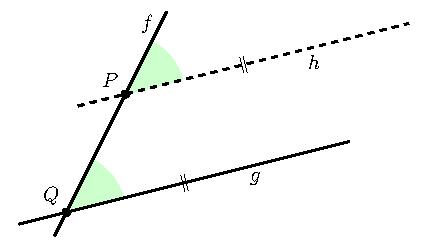
\includegraphics[width=0.5\linewidth, keepaspectratio]{figures/geometry-6.pdf}
    \caption{Situation aus \cref{prop:14.7}}
    \label{fig:bild-6}
\end{figure}

\begin{beweis}
    Sei $f \in G$ mit $P \in f$. Ist $f \cap g = \emptyset$, so setze
    $h := f$. Andernfalls sei $\Set{Q} : = f \cap g$.

    Sei $\varphi$ die eindeutige Isometrie mit $\varphi(Q) = P$,
    $\varphi(P) = P'$, die die Halbebenen bzgl. $f$ nicht vertauscht.
    
    Setze $h := \varphi(g)$.

    \underline{Z.~Z.:} $h \cap g = \emptyset$.

    Andernfalls sei $\Set{R} = h \cap g$.

    \begin{figure}[htp]
        \centering
        %\documentclass[varwidth=true, border=2pt]{standalone}
\usepackage{tkz-euclide}

\begin{document}
\usetkzobj{all}
\begin{tikzpicture}
    \tkzSetUpPoint[shape=circle,size=10,color=black,fill=black]
    \tkzSetUpLine[line width=1]
    \tkzDefPoints{0/0/Q, 2/0/P, 1/2/R}


    \pgfmathsetmacro{\firstAngle}{0}
    \pgfmathsetmacro{\secondAngle}{-120}
    \path[draw,red, fill=red!40] (Q) -- ++(\firstAngle:.4) arc[start angle=\firstAngle, delta angle=\secondAngle,radius=.4];

    \tkzMarkAngle[arc=l,size=0.8cm,color=green,fill=green!20](Q,R,P)
    \path[draw] ++(-50:.2) node[rotate=-50] {$\alpha$};
    \node at (1,1.5) {$\beta$};
    \tkzDrawLine(Q,P)
    \tkzDrawLine(Q,R)
    \tkzDrawLine(P,R)
    \tkzDrawPoints(P,Q,R)
    \tkzLabelPoint[below left](P){$P$}
    \tkzLabelPoint[above left](Q){$Q$}
    \tkzLabelPoint[above=0.2cm](R){$R$}
\end{tikzpicture}
\end{document}

        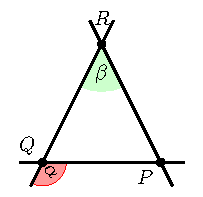
\includegraphics[width=0.5\linewidth, keepaspectratio]{figures/geometry-7.pdf}
        \caption{TODO}
        \label{fig:bild-6}
    \end{figure}
\end{beweis}

\begin{bemerkung}
    Jeder Innenwinkel eines Dreiecks ist kleiner als alle nicht-anliegenden
    Außenwinkel.
\end{bemerkung}

%!TEX root = GeoTopo.tex
%%%%%%%%%%%%%%%%%%%%%%%%%%%%%%%%%%%%%%%%%%%%%%%%%%%%%%%%%%%%%%%%%%%%%
% Mitschrieb vom 30.01.2014                                         %
%%%%%%%%%%%%%%%%%%%%%%%%%%%%%%%%%%%%%%%%%%%%%%%%%%%%%%%%%%%%%%%%%%%%%
\chapter{Krümmung}
\section{Krümmung von Kurven}\label{sec:Kurvenkrümmung}
\begin{definition}%In Vorlesung: Def.+Bem. 16.1
    Sei $\gamma: I = [a, b] \rightarrow \mdr^n$ eine $C^\infty$-Funktion.
    
    \begin{defenum}
        \item $\gamma$ heißt \textbf{durch Bogenlänge parametrisiert}\xindex{parametrisiert!durch Bogenlänge},
              wenn $\|\gamma'(t)\|_2 = 1$ für alle $t \in I$. Dabei
              ist $\gamma'(t) = \left (\gamma_1'(t), \gamma_2'(t), \dots, \gamma_n'(t) \right)$
        \item $l(\gamma) = \int_a^b \|\gamma'(t)\| \mathrm{d} t$ heißt
              \textbf{Länge von $\gamma$}\xindex{Kurve!Länge einer}
    \end{defenum}    
\end{definition}

\begin{bemerkung}[Eigenschaften von Kurven I]%In Vorlesung: Def.+Bem. 16.1
    Sei $\gamma: I = [a, b] \rightarrow \mdr^n$ eine $C^\infty$-Funktion.

    \begin{bemenum}
        \item Ist $\gamma$ durch Bogenlänge parametrisiert, so ist $l(\gamma) = b-a$.
        \item \label{bem:16.1d} Ist $\gamma$ durch Bogenlänge parametrisiert, so ist 
              $\gamma'(t)$ orthogonal zu $\gamma''(t)$ für alle $t \in I$.
    \end{bemenum}
\end{bemerkung}

\begin{beweis}
    von \cref{bem:16.1d}:

    $1 = \|\gamma'(t)\| = \|\gamma'(t)\|^2 = \langle \gamma'(t), \gamma'(t) \rangle$\\
    \begin{align*}
        \Rightarrow 0 &= \frac{\mathrm{d}}{\mathrm{d}t} \langle \gamma'(t), \gamma'(t) \rangle\\
                      &= \frac{\mathrm{d}}{\mathrm{d}t} (\gamma_1'(t)\gamma_1'(t) + \gamma_2'(t)\gamma_2'(t))\\
                      &= 2 (\gamma_1''(t) \cdot \gamma_1'(t) + \gamma_2''(t) \cdot \gamma_2'(t))\\
                      &= 2 \langle \gamma''(t), \gamma'(t) \rangle
     \end{align*}
\end{beweis}

\begin{definition}%In Vorlesung: Definition 16.2
    Sei $\gamma: I \rightarrow \mdr^2$ eine durch Bogenlänge
    parametrisierte Kurve.

    \begin{defenum}
        \item Für $t \in I$ sei $n(t)$ \textbf{Normalenvektor}\xindex{Normalenvektor}
              an $\gamma$ in $t$, d.~h.
              \[\langle n(t), \gamma'(t) \rangle = 0, \;\;\; \|n(t)\|=1 \]
              und $\det((\gamma_1(t), n(t))) = +1$
        \item Nach \cref{bem:16.1d} sind $n(t)$ und $\gamma''(t)$ linear
              abhängig, d.~h. es gibt $\kappa(t) \in \mdr$ mit
              \[\gamma''(t) = \kappa(t) \cdot n(t)\]
              $\kappa(t)$ heißt \textbf{Krümmung}\xindex{Krümmung}
              von $\gamma$ in $t$.
    \end{defenum}
\end{definition}

\begin{beispiel}%In Vorlesung: Beispiel 16.3
    Gegeben sei ein Kreis mit Radius $r$, d.~h. mit Umfang $2\pi r$.
    Es gilt:

    \[\gamma(t) = \left (r \cdot \cos \frac{t}{r}, r \cdot \sin \frac{t}{r} \right ) \text{ für } t \in [0, 2\pi r]\]
    ist parametrisiert durch Bogenlänge.

    \begin{align*}
        \gamma'(t)  &= \left ((r \cdot \frac{1}{r}) (- \sin \frac{t}{r}), r \frac{1}{r} \cos \frac{t}{r} \right )\\
                    &= \left (- \sin \frac{t}{r}, \cos \frac{t}{r} \right )\\
        \Rightarrow n(t) &= \left (- \cos \frac{t}{r}, - \sin \frac{t}{r} \right )\\
        \gamma''(t) &= \left (- \frac{1}{r} \cos \frac{t}{r}, - \frac{1}{r} \sin \frac{t}{r} \right )\\
                    &= \frac{1}{r} \cdot \left (- \cos \frac{t}{r}, - \sin \frac{t}{r} \right )\\
        \Rightarrow \kappa(t) &= \frac{1}{r}
    \end{align*}
\end{beispiel}

\begin{definition}%In Vorlesung: Def.+Bem. 16.4
    Sei $\gamma: I \rightarrow \mdr^3$ eine durch Bogenlänge parametrisierte
    Kurve.

    \begin{defenum}
        \item Für $t \in I$ heißt $\kappa(t) := \|\gamma''(t)\|$ die
              \textbf{Krümmung}\xindex{Krümmung} von $\gamma$ in $t$.
        \item Ist für $t \in I$ die Ableitung $\gamma''(t) \neq 0$,
              so heißt $\gamma''(t)$ \textbf{Normalenvektor}\xindex{Normalenvektor}
              an $\gamma$ in $t$.
        \item \label{def:16.4c} $b(t)$ sei ein Vektor, der $\gamma'(t), n(t)$
              zu einer orientierten Orthonormalbasis von $\mdr^3$ ergänzt.
              Also gilt:
              \[\det(\gamma'(t), n(t), b(t)) = 1\]
              $b(t)$ heißt \textbf{Binormalenvektor}\xindex{Binormalenvektor},
              die Orthonormalbasis 
              \[\Set{\gamma'(t), n(t), b(t)}\]
              heißt \textbf{begleitendes Dreibein}\xindex{Dreibein!begreitendes}.
    \end{defenum}
\end{definition}

\begin{bemerkung}[Eigenschaften von Kurven II]%In Vorlesung: Def.+Bem 16.4
    Sei $\gamma: I \rightarrow \mdr^3$ durch Bogenlänge parametrisierte
    Kurve.

    \begin{bemenum}
        \item $n(t)$ ist orthogonal zu $\gamma'(t)$.
        \item $b(t)$ aus \cref{def:16.4c} ist eindeutig.
    \end{bemenum}
\end{bemerkung}

\section{Tangentialebene}
Erinnerung Sie sich an \cref{def:8.5} \enquote{reguläre Fläche}.

Äquivalent dazu ist: $S$ ist lokal von der Form
\[V(f) = \Set{x \in \mdr^3 | f(x) = 0 }\]
für eine $C^\infty$-Funktion $f: \mdr^\infty \rightarrow \mdr$.\todo{Wirklich $\mdr^\infty$?}

\begin{definition}%In Vorlesung: 17.1
    Sei $S \subseteq \mdr^3$ eine reguläre Fläche, $s \in S$,
    $F: U \rightarrow V \cap S$ eine lokale Parametrisierung um $s$
    (d.~h. $s \in V$)
    \[(u,v) \mapsto (x(u,v), y(u,v), z(u,v))\]
    Für $p=F^{-1}(s) \in U$ sei
    \[        J_F(u,v) = \begin{pmatrix}
            \frac{\partial x}{\partial u} (p) & \frac{\partial x}{\partial v} (p)\\
            \frac{\partial y}{\partial u} (p) & \frac{\partial y}{\partial v} (p)\\
            \frac{\partial z}{\partial u} (p) & \frac{\partial z}{\partial v} (p)
        \end{pmatrix}\]
    und $D_P F: \mdr^2 \rightarrow \mdr^3$ die durch $J_F (p)$
    definierte lineare Abbildung.

    Dann heißt $T_s S := \Bild(D_p F)$ die \textbf{Tangentialebene}\xindex{Tangentialebene}
    an $s \in S$.
\end{definition}

\begin{bemerkung}%In Vorlesung: 17.2
    $T_s S$ ist $2$-dimensionaler Untervektorraum von $\mdr^3$.
\end{bemerkung}

\begin{bemerkung}%In Vorlesung: 17.3
    $T_s S$ hängt nicht von der gewählten Parametrisierung ab.
\end{bemerkung}

\begin{beweis}\leavevmode
    \begin{behauptung}
        $T_s S = \Set{x \in \mdr^3 | \exists \text{parametrisierte Kurve } \gamma:[- \varepsilon, + \varepsilon] \rightarrow S \text{ für ein } \varepsilon > 0 \text{ mit } \gamma(0) = S \text{ und } \gamma'(0) = x}$
    \end{behauptung}
\end{beweis}

%%%%%%%%%%%%%%%%%%%%%%%%%%%%%%%%%%%%%%%%%%%%%%%%%%%%%%%%%%%%%%%%%%%%%
% Mitschrieb vom 04.02.2014                                         %
%%%%%%%%%%%%%%%%%%%%%%%%%%%%%%%%%%%%%%%%%%%%%%%%%%%%%%%%%%%%%%%%%%%%%
\begin{bemerkung}%In Vorlesung: Bemerkung 17.4
    Sei $S=V(f)$ eine reguläre Fläche in $\mdr^3$, also 
    $f:V \rightarrow \mdr$ eine $C^\infty$-Funktion, $V \subseteq \mdr^3$
    offen, $\grad(f)(x) \neq 0$ für alle $x \in S$.

    Dann ist $T_s S = (\grad(f)(s))^\perp$ für jedes $s \in S$.
\end{bemerkung}
\begin{beweis}
    Sei $x \in T_s S, \gamma:[-\varepsilon, +\varepsilon] \rightarrow S$
    eine parametrisierte Kurve mit $\varepsilon > 0$ und $\gamma'(0) = s$,
    sodass $\gamma'(0) = x$ gilt. Da $\gamma(t) \in S$ für alle
    $t \in [-\varepsilon, \varepsilon]$, ist $f \circ \gamma = 0$\\
    $\Rightarrow 0 = (f \circ \gamma)'(0) = \langle \grad(f)(\gamma(0)), \gamma'(0) \rangle$\\
    $\Rightarrow T_s S \subseteq \grad (f)(s)^\perp$\\
    $\xRightarrow{\dim = 2} T_s S = (\grad(f)(s))^\perp$
\end{beweis}

\begin{definition}%In Vorlesung: Def.+Bem 17.5
    \begin{defenum}
        \item Ein \textbf{Normalenfeld}\xindex{Normalenfeld} auf der
              Fläche $S$ ist eine Abbildung $n: S \rightarrow S^2 \subseteq \mdr^3$
              mit $n(s) \in T_s S^\perp$ für jedes $s \in S$.
        \item $S$ heißt \textbf{orientierbar}\xindex{Fläche!orientierbare},
              wenn es ein stetiges Normalenfeld auf $S$ gibt.
    \end{defenum}
\end{definition}

Manchmal wird zwischen einem \textit{Normalenfeld} und einem
\textit{Einheitsnormalenfeld}\xindex{Einheitsnormalenfeld} unterschieden.
Im folgenden werden diese Begriffe jedoch synonym benutzt.

\begin{bemerkung}[Eigenschaften von Normalenfeldern]%In Vorlesung: Def.+Bem 17.5
    \begin{bemenum}
        \item Ein Normalenfeld auf $S$ ist genau dann stetig, wenn es
              glatt ist (also $C^\infty$).
        \item Zu jedem $s \in S$ gibt es eine Umgebung $V \subseteq \mdr^3$
              von $s$ und eine lokale Parametrisierung $F: U \rightarrow V$
              von $S$ um $s$, sodass auf $F(U) = V \cap S$
              ein stetiges Normalenfeld existiert.
        \item $S$ ist genau dann orientierbar, wenn es einen 
              differenzierbaren Atlas von $S$ aus lokalen Parametrisierungen
              $F_i: U_i \rightarrow V_i,\;i \in I$ gibt, sodass
              für alle $i, j \in F$ und alle $s \in V_i \cap V_j \cap S$
              gilt:
              \[\det(\underbrace{D_s \overbrace{F_j \circ F_i^{-1}}^{V_i \rightarrow V_j}}_{\in \mdr^{3 \times 3}})\]
    \end{bemenum}
\end{bemerkung}

\begin{beweis}
    Wird hier nicht geführt.%TODO: Übung? Übungsblatt?
\end{beweis}

\begin{beispiel}
    \begin{bspenum}
        \item $S = S^2$, $n_1 = \id_{S^2}$ ist stetiges Normalenfeld.\\
              $n_2 = - \id_{S^2}$ ist auch stetiges Normalenfeld.
        \item $S = \text{Möbiusband}$ (vgl. \cref{fig:moebius-strip})
              ist nicht orientierbar. Es existiert ein Normalenfeld,
              aber kein stetiges Normalenfeld.
    \end{bspenum}
\end{beispiel}

\begin{figure}[htp]\xindex{Möbiusband}
    \centering
    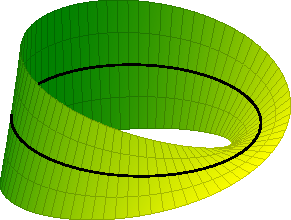
\includegraphics[width=0.5\linewidth, keepaspectratio]{figures/moebius-strip.pdf} 
    \caption{Möbiusband}
    \label{fig:moebius-strip}
\end{figure}

\section{Gauß-Krümmung}
\begin{bemerkung}\label{bem:18.1}%In Vorlesung: Bemerkung 18.1
    Sei $S$ eine reguläre Fläche, $s \in S$, $n(s)$ ist ein Normalenvektor
    in $s$, $x \in T_s (S)$, $\|x\| = 1$.

    Sei $E$ der von $x$ und $n(s)$ aufgespannte 2-dimensionale 
    Untervektorraum von $\mdr^3$.

    Dann gibt es eine Umgebung $V \subseteq \mdr^3$ von $s$, sodass
    \[C := (s + E) \cap S \cap V\]
    das Bild einer durch Bogenlänge parametrisierten Kurve
    $\gamma:[-\varepsilon, \varepsilon] \rightarrow s$ enthält mit
    $\gamma(0) = s$ und $\gamma'(0) = x$.
\end{bemerkung}

\begin{beweis}
    \enquote{Satz über implizite Funktionen}, siehe z.~B. 
    \href{https://github.com/MartinThoma/LaTeX-examples/tree/master/documents/Analysis\%20II}{\path{github.com/MartinThoma/LaTeX-examples/tree/master/documents/Analysis\%20II}}
\end{beweis}

\begin{definition}\xindex{Normalenkrümmung}%In Vorlesung: Definition 18.2
    In der Situation aus \cref{bem:18.1} heißt die Krümmung $\kappa_\gamma(0)$
    der Kurve $\gamma$ in der Ebene $(s+ E)$ im Punkt $s$ die
    \textbf{Normalenkrümmung}\footnotemark von $S$ in $s$ in Richtung
    $x = \gamma'(0)$.

    Man scheibt: $\kappa_\gamma(0) := \kappanor(s, x)$
\end{definition}
\footnotetext{Die Krümmung ist nur bis auf das Vorzeichen bestimmt.}

\begin{beispiel}%In Vorlesung: Beispiel 18.3
    \begin{bspenum}
        \item $S = S^2 = V(X^2 + Y^2 + Z^2 - 1)$ ist die Kugel um den Ursprung mit Radius~1,
              $n = \id$, $s=(0,0,1)$, $x=(1,0,0)$\\
              $\Rightarrow E = \mdr \cdot x + \mdr \cdot n(s)$ ($x,z\text{-Ebene}$)

              $C = E \cap S$ ist Kreislinie\\
              $\kappanor(s, x) = \frac{1}{r} = 1$
        \item $S = V(X^2 + Z^2 - 1) \subseteq \mdr^3$ ist ein Zylinder (siehe \cref{fig:regular-zylinder}).
              $s = (1,0,0)$\\
              $x_1 = (0,1,0) \Rightarrow E_1 = \mdr \cdot e_1 + \mdr \cdot e_2$ ($x,y\text{-Ebene}$)\\
              $S \cap E_1 = V(X^2 + Y^2 - 1) \cap E$, Kreislinie in $E$\\
              $\Rightarrow \kappanor(s, x_1) = \pm 1$\\
              $x_2 = (0, 0, 1), E_2 = \mdr \cdot e_1 + \mdr \cdot e_3$ ($x,z\text{-Ebene}$)\\
              $V \cap E_2 \cap S = \Set{(1, 0, z) \in \mdr^3 | z \in \mdr}$ ist eine Gerade\\
              $\Rightarrow \kappanor(s, x_2) = 0$
        \item $S = V(X^2 - Y^2 - Z)$, $s = (0,0,0)$ (Hyperbolisches Paraboloid\xindex{Paraboloid!hyperbolisches}, siehe \cref{fig:hyperbolic-paraboloid})\\
              $x_1 = (1,0,0)$, $n(s) = (0,0,1)$\\
              $x_2 = (0, 1, 0)$\\
              $\kappanor(s, x_1) = 2$\\
              $\kappanor(s, x_2) = -2$
    \end{bspenum}
\end{beispiel}

\begin{figure}[ht]
    \centering
    \subfloat[$S = V(X^2 + Z^2 - 1)$]{
        \resizebox{0.4\linewidth}{!}{\pgfplotsset{
    colormap={whitered}{
        color(0cm)=(white);
        color(1cm)=(orange!75!red)
    }
}
\begin{tikzpicture}
    \begin{axis}[
    colormap name=whitered,
    width=15cm,
    view={340}{25},
    enlargelimits=false,
    grid=major,
    domain=0:5,
    y domain=0:2*pi,
    xmin=-1.5, xmax=1.5,
    ymin=-1.5, ymax=1.5,  zmin=0.0,
    samples=30, %57 : TeX capacity exceeded, sorry [main memory size=3000000].
                % see also http://tex.stackexchange.com/a/7954/5645
    xlabel=$x$,
    ylabel=$y$,
    zlabel={$z$},
    %colorbar,
    colorbar style={
        at={(-0.1,0)},
        anchor=south west,
        height=0.25*\pgfkeysvalueof{/pgfplots/parent axis height},
        title={$f(x,y)$}
    }
    ]
    \addplot3 [surf,z buffer=sort] ({cos(deg(y))},{sin(deg(y))},{x});
    \end{axis}
\end{tikzpicture}
}
        \label{fig:regular-zylinder}
    }%
    \subfloat[$S = V(X^2 - Y^2 - Z)$]{
        \resizebox{0.4\linewidth}{!}{\documentclass[border=2pt]{standalone}
\usepackage{pgfplots}
\pgfplotsset{compat=1.9} %It is possible to remove this line, but you will get a warning

\begin{document}
\pgfplotsset{
    colormap={whitered}{
        color(0cm)=(white);
        color(1cm)=(orange!75!red)
    }
}
\begin{tikzpicture}
    \begin{axis}[
    colormap name=whitered,
    width=15cm,
    view={340}{25},
    enlargelimits=false,
    grid=major,
    domain=-2:2,
    y domain=-2:2,
    samples=40, %57 : TeX capacity exceeded, sorry [main memory size=3000000].
                % see also http://tex.stackexchange.com/a/7954/5645
    xlabel=$x$,
    ylabel=$y$,
    zlabel={$z$},
    colorbar,
    colorbar style={
        at={(-0.1,0)},
        anchor=south west,
        height=0.25*\pgfkeysvalueof{/pgfplots/parent axis height},
        title={$f(x,y)$}
    }
    ]
    \addplot3[surf,draw=black] {x^2-y^2};
    \end{axis}
\end{tikzpicture}
\end{document}
}
        \label{fig:hyperbolic-paraboloid}
    }%
    \label{fig:regular-surfaces}
    \caption{Beispiele für reguläre Flächen}
\end{figure}

%%%%%%%%%%%%%%%%%%%%%%%%%%%%%%%%%%%%%%%%%%%%%%%%%%%%%%%%%%%%%%%%%%%%%
% Mitschrieb vom 06.02.2014                                         %
%%%%%%%%%%%%%%%%%%%%%%%%%%%%%%%%%%%%%%%%%%%%%%%%%%%%%%%%%%%%%%%%%%%%%
\begin{definition}\label{def:18.4}\xindex{Normalenkrümmung}%In Vorlesung: Def. 18.4
    Sei $S \in \mdr^3$ eine reguläre Fläche, $s \in S$, ($n$ ein
    stetiges Normalenfeld auf $S$)

    $\gamma:[-\varepsilon, \varepsilon] \rightarrow S$ eine nach
    Bogenlänge parametrisierte Kurve ($\varepsilon > 0$) mit
    $\gamma(0) = s$ und $\gamma''(0) \neq 0$.

    Sei $n(0) := \frac{\gamma''(0)}{\|\gamma''(0)\|}$. Zerlege
    $n(0) = n(0) + n(0)^\bot$ mit $n(0)^\bot \in T_s S$ und
    $n(0)^\bot \in (T_s S)^\bot$.

    Dann ist $n(0)^\bot = \langle n(0), n(s) \rangle \cdot n(s)$\\
    $\kappanor(s, \gamma) := \langle \gamma''(0), n(s) \rangle$
    die \textbf{Normalenkrümmung}.\todo{Ist das hier die Normalenkrümmung? Was ist mit der anderen Def.?}
\end{definition}

\begin{bemerkung}
    Sei $\overline{\gamma}(t) = \gamma(-t)$, $t \in [- \varepsilon, \varepsilon]$.
    Dann ist $\kappanor(s, \overline{\gamma}) = \kappanor(s, \gamma)$.
\end{bemerkung}

\begin{beweis}
    $\overline{\gamma}''(0) = \gamma''(0)$, da $\overline{\gamma}'(0) = - \gamma'(0)$.

    Es gilt: $\kappanor(s,\gamma)$ hängt nur von $|\gamma'(0)|$ ab
    und ist gleich $\kappanor(s, \gamma'(0))$.
\end{beweis}

\begin{bemerkung}%In Vorlesung: Bem.+Def. 18.6
    Sei $S$ eine reguläre Fläche und $n=n(s)$ ein Normalenvektor an 
    $S$ in $s$.

    Sei $T_{s}^{1} S = \Set{x \in T_s S | \|x\| = 1} \cong S^1$.
    Dann ist $\kappanor^n(s): T_s S \rightarrow \mdr$,
    $x \mapsto \kappanor(s,x)$ eine glatte Funktion und 
    $\Bild \kappanor(s)$ ist ein abgeschlossenes Intervall.
\end{bemerkung}

\begin{definition}\xindex{Hauptkrümmung}\xindex{Gauß-Krümmung}%In Vorlesung: Bem.+Def. 18.6
    Sei $S$ eine reguläre Fläche und $n=n(s)$ ein Normalenvektor an 
    $S$ in $s$.

    \begin{defenum}
        \item $\kappa^n_1(s) := \min \Set{\kappanor^n(s,x) | x \in T_s^1 S}$ und\\
              $\kappa^n_2(s) := \max \Set{\kappanor^n(s,x) | x \in T_s^1 S}$
              heißen \textbf{Hauptkrümmungen} von $S$ in $s$.
        \item $K(s) := \kappa_1^n(s) \cdot \kappa_2^n(s)$ heißt
              \textbf{Gauß-Krümmung} von $S$ in $s$.
    \end{defenum}
\end{definition}

\begin{bemerkung}%In Vorlesung: Bem.+Def. 18.6
    Ersetzt man $n$ durch $-n$, so gilt: $\kappanor^{-n}(s, x) = - \kappanor^n(x)\; \forall x \in T_s^1 S$\\
    $\Rightarrow \kappa_1^{-n}(s) = - \kappa_2^n(s)$,\\
    $\kappa_2^{-n}(s) = - \kappa_1^n (s)$\\
    und $K^{-n}(s) = K^n(s) =: K(s)$.
\end{bemerkung}

\begin{beispiel}
    \begin{bspenum}
        \item $S = S^2$. Dann ist $\kappa_1(s) = \kappa_2(s) = \pm 1\;\forall s \in S^2$\\
              $\Rightarrow K(s) = 1$
        \item Zylinder:\\
              $\kappa_1(s) = 0, \kappa_2(s) = 1 \Rightarrow K(s) = 0$
        \item Sattelpunkt auf hyperbolischem Paraboloid:\\
              $\kappa_1(s) < 0, \kappa_2(s) = 0 \rightarrow K(s) < 0$
        \item $S = \text{Torus}$. Siehe \cref{fig:torus-gauss-kruemmung}\\
            \begin{figure}[htp]\xindex{Torus}
                \centering
                % The following answers were used to create this image:
% - http://tex.stackexchange.com/a/373/5645 - Torus
\documentclass[border=2pt]{standalone}
\usepackage{amsmath,amssymb}
\usepackage{tikz}
\usetikzlibrary{patterns,arrows,positioning}

\begin{document}
\begin{tikzpicture}
\tikzstyle{point}=[circle,thick,draw=black,fill=black,inner sep=0pt,minimum width=4pt,minimum height=4pt]
\draw (-3.5,0) .. controls (-3.5,2) and (-1.5,2.5) .. (0,2.5);
\draw[xscale=-1] (-3.5,0) .. controls (-3.5,2) and (-1.5,2.5) .. (0,2.5);
\draw[rotate=180] (-3.5,0) .. controls (-3.5,2) and (-1.5,2.5) .. (0,2.5);
\draw[yscale=-1] (-3.5,0) .. controls (-3.5,2) and (-1.5,2.5) .. (0,2.5);

\draw (-2,.2) .. controls (-1.5,-0.3) and (-1,-0.5) .. (0,-.5) .. controls (1,-0.5) and (1.5,-0.3) .. (2,0.2);
\draw (-1.75,0) .. controls (-1.5,0.3) and (-1,0.5) .. (0,.5) .. controls (1,0.5) and (1.5,0.3) .. (1.75,0);

\draw[dashed] (2.65,0) ellipse (0.85 and 0.6);
\draw (3.5,0) arc (-360:-180:0.85 and 0.6);

\node (s1)[point,orange,label={[label distance=0mm]\color{orange}$s_1$}] at (3.5,0) {};
\node (s2)[point,red,label={[label distance=0mm]\color{red}$s_2$}] at (2.8,0.6) {};
\node (s3)[point,green,label={[label distance=0mm]\color{green}$s_3$}] at (1.8,0) {};
\draw[red] (0,0.07) ellipse (3cm and 1.5cm);
\end{tikzpicture}
\end{document}
 
                \caption{$K(s_1) > 0$, $K(s_2) = 0$, $K(s_3) < 0$}
                \label{fig:torus-gauss-kruemmung}
            \end{figure}
    \end{bspenum}
\end{beispiel}

\begin{bemerkung}%In Vorlesung: Bem. 18.7
    Sei $S$ eine reguläre Fläche, $s \in S$ ein Punkt.
    \begin{bemenum}
        \item Ist $K(s) > 0$, so liegt $S$ in einer Umgebung von $s$
              ganz auf einer Seite von $T_s S + s$.
        \item Ist $K(s) < 0$, so schneidet jede Umgebung von $s$ in $S$
              beide Seiten von $T_s S + s$.
    \end{bemenum}
\end{bemerkung}

%%%%%%%%%%%%%%%%%%%%%%%%%%%%%%%%%%%%%%%%%%%%%%%%%%%%%%%%%%%%%%%%%%%%%
% Mitschrieb vom 11.02.2014                                         %
%%%%%%%%%%%%%%%%%%%%%%%%%%%%%%%%%%%%%%%%%%%%%%%%%%%%%%%%%%%%%%%%%%%%%
\section{Erste und zweite Fundamentalform}%In Vorlesung: §19
Sei $S \subseteq \mdr^3$ eine reguläre Fläche, $s \in S$, $T_s S$ die Tangentialebene
an $S$ in $s$.

\begin{bemerkung}%In Vorlesung: Bem.+Def. 19.1
    \begin{bemenum}
        \item \label{bem:19.1a} Die Einschränkung des Standardskalarproduktes des $\mdr^3$ auf
              $T_s S$ macht $T_s S$ zu einem euklidischen Vektorraum.
        \item Sei $F: U \rightarrow V$ eine lokale Parametrisierung von $S$ um
              $s$ und $p := F^{-1}(s)$.

              Dann ist $\Set{D_P F(e_1), D_P F(e_2)}$ eine Basis von $T_s S$.
        \item Bzgl. der Basis $\Set{D_P F(e_1), D_P F(e_2)}$ hat das 
              Standardskalarprodukt aus \cref{bem:19.1a} die Darstellungsmatrix
              \begin{align*}
                I_S &= \begin{pmatrix}
                          g_{1,1}(s) & g_{1,2}(s)\\
                          g_{1,2}(s) & g_{2,2}(s)
                       \end{pmatrix} =
                       \begin{pmatrix}
                          E(s) & F(s) \\
                          F(s) & G(s)
                       \end{pmatrix}\\
       \text{mit } g_{i,j} &= g_s(D_P F(e_i), D_P F(e_j))\\
                      &= \langle \frac{\partial F}{\partial u_i} (p), \frac{\partial F}{\partial u_j} (p) \rangle \;\;\; i,j \in \Set{1,2}
              \end{align*}
              Die Matrix $I_S$ heißt \textbf{erste Fundamentalform}\xindex{Fundamentalform!erste}
              von $S$ bzgl. der Parametrisierung $F$.
        \item $g_{i,j}(s)$ ist eine differenzierbare Funktion von $s$.
    \end{bemenum}
\end{bemerkung}

\begin{bemerkung}
    \[\det(I_S) = \left \| \frac{\partial F}{\partial u_1}(p) \times \frac{\partial F}{\partial u_2}(p) \right \|^2\] 
\end{bemerkung}

\begin{beweis}
    Sei $\frac{\partial F}{\partial u_1}(p) = \begin{pmatrix}
        x_1\\ x_2 \\ x_3
    \end{pmatrix}, \;\;\; \frac{\partial F}{\partial u_2}(p) = \begin{pmatrix}
        y_1\\ y_2 \\ y3
    \end{pmatrix}$

    Dann ist $\frac{\partial F}{\partial u_1}(p) \times \frac{\partial F}{\partial u_2}(p) = \begin{pmatrix}
        z_1 \\ z_2 \\ z_3
    \end{pmatrix}$ mit
    \begin{align*}
        z_1 &= x_2 y_3 - x_3 - y_2\\
        z_2 &= x_3 y_1 - x_1 y_3\\
        z_3 &= x_1 y_2 - x_2 y_1\\
    \Rightarrow \|\frac{\partial F}{\partial u_1} (p) \times \frac{\partial F}{\partial u_2} (p)\| &= z_1^2 + z_2^2 + z_3^2\\
    \end{align*}
    \begin{align*}
        \det(I_S) &= g_{1,1} g_{2,2} - g_{1,2}^2\\
        &= \left \langle \begin{pmatrix} x_1 \\ x_2 \\ x_3 \end{pmatrix}, \begin{pmatrix} x_1 \\ x_2 \\ x_3 \end{pmatrix} \right \rangle \left \langle \begin{pmatrix} y_1 \\ y_2 \\ y_3 \end{pmatrix}, \begin{pmatrix} y_1 \\ y_2 \\ y_3 \end{pmatrix} \right \rangle - \left \langle \begin{pmatrix} x_1 \\ x_2 \\ x_3 \end{pmatrix}, \begin{pmatrix} y_1 \\ y_2 \\ y_3 \end{pmatrix} \right \rangle^2\\
        &= (x_1^2 + x_2^2 + x_3^2) (y_1^2 + y_2^2 + y_3^2) - (x_1 y_1 + x_2 y_2 + x_3 y_3)^2
    \end{align*}
\end{beweis}

\begin{definition}\xindex{Flächenelement}%In Vorlesung: Def.+Bem. 19.3 / Erinnerung
    \begin{defenum}
        \item Das Differential
              \[\mathrm{d} A = \sqrt{\det (I)} \mathrm{d} u_1 \mathrm{d} u_2\]
              heißt \textbf{Flächenelement} von $S$ bzgl. der Parametrisierung $F$.
        \item \label{def:berechenbares-integral}Für eine Funktion $f: V \rightarrow \mdr$ heißt 
              \[\int_V f \mathrm{d} A := \int_U f(\underbrace{F(u_1, u_2)}_{=: s}) \sqrt{\det I(s)} \mathrm{d} u_1 \mathrm{d} u_2\]
              der \textbf{Wert des Integrals} von $f$ über $V$, falls das Integral rechts
              existiert.
    \end{defenum}

\end{definition}

\begin{bemerkung}
    \begin{bemenum}
        \item $\int_V f \mathrm{d} A$ ist unabhänig von der gewählten Parametrisierung.
        \item Sei $f: S \rightarrow \mdr$ eine Funktion, die im Sinne von
              \cref{def:berechenbares-integral} lokal integrierbar ist.

              Dann ist $\int_S f \mathrm{d} A$ wohldefiniert, falls (z.~B.) $S$
              kompakt ist.

              Etwa: $\int_S f \mathrm{d} A = \sum_{i=1}^n \int_{V_i} f \mathrm{d} A - \sum_{i \neq j} \int_{V_i \cap V_j} f \mathrm{d} A + \sum_{i,j,k} \int_{V_i \cap V_j \cap V_k} - \dots$
    \end{bemenum}
\end{bemerkung}

\begin{beweis}
    \begin{enumerate}[label=\alph*)]
        \item Mit Transformationsformel
        \item Ist dem Leser überlassen
    \end{enumerate}
\end{beweis}

\begin{proposition}
    Sei $S \subseteq \mdr^3$ eine reguläre, orientierbare Fläche mit glatten
    Normalenfeld $n: S \rightarrow S^2$. Dann gilt:

    \begin{propenum}
        \item $n$ induziert für jedes $s \in S$ eine lineare Abbildung $d_S n: T_s S \rightarrow T_{n(s)} S^2$
              durch 
              \[d_s n(x) = \frac{\mathrm{d}}{\mathrm{d} t} n (\underbrace{s \text{\enquote{+}} tx}_{\mathclap{\text{Soll auf Fläche $S$ bleiben}}}) \Bigr |_{t=0}\]
        \item $T_{n(s)} S^2 = T_s S$.
        \item $d_S n$ ist ein Endomorphismus von $T_s S$.
        \item $d_S n$ ist selbstadjungiert bzgl. des Skalarproduktes $I_S$.
    \end{propenum}
\end{proposition}

\begin{beweis}\leavevmode
    \begin{enumerate}[label=\alph*)]
        \item TODO
        \item $T_{n(S)} S^2 = \langle n(s) \rangle^\bot = T_s S$
        \item TODO
        \item Zu zeigen: $\forall x,y \in I_s S: \langle x, d_s n (y) \rangle = \langle d_s n(x), y \rangle$

        Aufgrund der Bilinearität des Skalarproduktes genügt es diese Eigenschaft
        für die Basisvektoren zu zeigen.

        Sei $x_i = D_P F(e_i) = \frac{\partial F}{\partial u_i} (p)\;\;\; i = 1,2$

        \underline{Beh.:} $\langle x_i, d_s n(x_j) \rangle = \langle \frac{\partial^2 F}{\partial u_i \partial u_j} (p), d_s n (x_i) \rangle$

        $\Rightarrow \langle \frac{\partial^2 F}{\partial u_i \partial u_j} (p), d_s n (x_i) \rangle = \langle x_j, d_s n (x_i) \rangle$

        \underline{Bew.:} 

        \begin{align*}
            0 &= \hphantom{\frac{\mathrm{d}}{\mathrm{d}t} \left (\right.} \langle \frac{\partial F}{\partial u} (p + t e_j), n(p + t e_j) \rangle\\
\Rightarrow 0 &= \frac{\mathrm{d}}{\mathrm{d}t} \left (\langle \frac{\partial F}{\partial u} (p + t e_j), n(p + t e_j) \rangle \right) \Bigr |_{t=0}\\
              &= \langle \underbrace{\frac{\mathrm{d}}{\mathrm{d}t} \frac{\partial F}{\partial u_i} (p + t e_j)}_{\frac{\partial^2 F}{\partial u_j \partial u_i} (p)} \Bigr |_{t=0}, n(s) \rangle + \langle x_i, d_s n \underbrace{D_P F (e_j)}_{x_j}\rangle
        \end{align*}
    \end{enumerate}
\end{beweis}

%%%%%%%%%%%%%%%%%%%%%%%%%%%%%%%%%%%%%%%%%%%%%%%%%%%%%%%%%%%%%%%%%%%%%
% Mitschrieb vom 13.02.2014                                         %
%%%%%%%%%%%%%%%%%%%%%%%%%%%%%%%%%%%%%%%%%%%%%%%%%%%%%%%%%%%%%%%%%%%%%
\begin{definition}\xindex{Fundamentalform!zweite}%In Vorlesung: Def. + Bem. 19.5 a)
    Die durch $-d_s n$ definierte symmetrische Bilinearform auf $T_s S$ heißt
    \textbf{zweite Fundamentalform} von $S$ in $s$ bzgl. $F$.

    Man schreibt: $II_s(x,y) =  \langle - d_s n(x), y \rangle = I_s (-d_s n(x), y)$
\end{definition}

\begin{bemerkung}%%In Vorlesung: Def. + Bem. 19.5 b)
    Bezüglich der Basis $\Set{x_1, x_2}$ von $T_s S$ hat $II_s$ die Darstellungsmatrix
    \[(h^{(s)}_{i,j})_{i,j=1,2} \text{ mit } h_{i,j}(s) = \langle \frac{\partial^2 F}{\partial u_i \partial u_j} (p), n(s) \rangle \]
\end{bemerkung}

\begin{proposition}\label{prop:19.6}%In Vorlesung: Proposition 19.6
    Sei $\gamma:[- \varepsilon, \varepsilon] \rightarrow S$ eine nach Bogenlänge
    parametrisierte Kurve mit $\gamma(0) = s$. Dann gilt:
    \[\kappanor(s, \gamma) = II_s(\gamma'(0), \gamma'(0))\]
\end{proposition}

\begin{beweis}
    Nach \cref{def:18.4} ist $\kappanor(s, \gamma) = \langle \gamma''(0), n(s) \rangle$.
    Nach Voraussetzung ist $n(\gamma(t)) \perp \gamma'(t) \Leftrightarrow \langle \gamma''(0), n(s) \rangle = 0$.
    Die Ableitung nach $t$ ergibt 
    \begin{align*}
        0 &= \frac{\mathrm{d}}{\mathrm{d}t}(\langle n (\gamma(t)), \gamma'(t))\\
        &= \left \langle \frac{\mathrm{d}}{\mathrm{d}t} n(\gamma(t)) \Bigr |_{t=0}, \gamma'(0) \right \rangle + \langle n(s), \gamma''(0) \rangle\\
        &= \langle d_s n (\gamma'(0)), \gamma'(0) \rangle + \kappa(s,\gamma)\\
        &= - II_s(\gamma'(0), \gamma'(0)) + \kappa(s, \gamma)
    \end{align*}
\end{beweis}

\begin{folgerung}\xindex{Normalkrümmung}%In Vorlesung: Folgerung 19.7
    Die beiden Definitionen von Normalkürmmung in \cref{sec:Kurvenkrümmung} stimmen
    überein:
    \[\kappanor(s, \gamma) = \kappanor(s, \gamma'(0))\]
\end{folgerung}

\begin{satz}%In Vorlesung: Satz 19.8
    Sei $S \subseteq \mdr^3$ eine reguläre, orientierbare Fläche und $s \in S$.
    \begin{satzenum}
        \item Die Hauptkrümmungen $\kappa_1(s), \kappa_2(s)$ sind die Eigenwerte
              von $II_s$.
        \item Für die Gaußkrümmung gilt: $K(s) = \det(II_s)$
    \end{satzenum}
\end{satz}

\begin{beweis}\leavevmode
    \begin{enumerate}[label=\alph*)]
        \item $II_s$ ist symmetrisch, $I_s S$ hat also eine Orthonormalbasis aus
              Eigenvektoren $y_1, y_2$ von $II_s$. Ist $x \in T_s S$, $\|x\| = 1$,
              so gibt es $\varphi \in [0,2\pi)$ mit $x = \cos \varphi \cdot y_1 + \sin \varphi \cdot y_2$.

              Seien $\lambda_1, \lambda_2$ die Eigenwerte von $II_s$, also 
              $II_s(y_i, y_i) = \lambda_i$. Dann gilt:
              \begin{align*}
                  II_s (x,x) &= \cos^2 \varphi \lambda_1 + \sin^2 \varphi \lambda_2\\
                  &= (1- \sin^2 \varphi) \lambda_1 + \sin^2 \varphi \lambda_2\\
                  &= \lambda_1 + \sin^2 \varphi (\lambda_2 - \lambda_1) \geq \lambda_1\\
                  &= \cos^2 \varphi + (1 - \cos^2 \varphi) \lambda_2\\
                  &= \lambda_2 - \cos^2 \varphi (\lambda_2 - \lambda_1) \leq \lambda_2\\
                  \xRightarrow{\crefabbr{prop:19.6}} \lambda_1 &= \min \Set{\kappanor (s,x) | x \in T^1_s S}\\
                  \lambda_2 &= \max \Set{\kappanor (s,x) | x \in T^1_s S}
              \end{align*}
    \end{enumerate}
\end{beweis}

\begin{satz}[Satz von Gauß-Bonnet]\xindex{Satz von!Gauß-Bonnet}
    Sei $S \subseteq \mdr^3$ eine kompakte, reguläre Fläche. Dann gilt:
    \[\int_S K(s) \mathrm{d}A = 2 \pi \chi(S)\]
    Dabei ist $\chi(S)$ die Euler-Charakteristik von $S$.
\end{satz}

\begin{beweis}
    Der Beweis wird hier nicht geführt. Er kann in \enquote{Elementare Differentialgeometrie}
    von Christian Bär (2. Auflage), ISBN 978-3-11-022458-0, ab Seite 281 nachgelesen werden.
\end{beweis}
%!TEX root = GeoTopo.tex
\chapter*{Lösungen der Übungsaufgaben\markboth{Lösungen der Übungsaufgaben}{Lösungen der Übungsaufgaben}}
\addcontentsline{toc}{chapter}{Lösungen der Übungsaufgaben}
\begin{solution}[\ref{ub1:aufg1}]
    \textbf{Teilaufgabe a)} Es gilt:
    \begin{enumerate}[label=(\roman*)]
        \item $\emptyset, X \in \fT_X$.
        \item $\fT_X$ ist offensichtlich unter Durchschnitten abgeschlossen,
              d.~h. es gilt für alle $U_1, U_2 \in \fT_X: U_1 \cap U_2 \in \fT_X$.
        \item Auch unter beliebigen Vereinigungen ist $\fT_X$ abgeschlossen,
              d.~h. es gilt für eine beliebige Indexmenge $I$ und alle
              $U_i \in \fT_X$ für alle $i \in I: \bigcup_{i \in I} U_i \in \fT_X$
    \end{enumerate}

    Also ist $(X, \fT_X)$ ein topologischer Raum.

    \textbf{Teilaufgabe b)} Wähle $x=1, y=0$. Dann gilt $x \neq y$
    und die einzige Umgebung von $x$ ist $X$. Da $y=0 \in X$ können
    also $x$ und $y$ nicht durch offene Mengen getrennt werden.
    $(X, \fT_X)$ ist also nicht hausdorffsch.

    \textbf{Teilaufgabe c)} Nach Bemerkung \ref{Trennungseigenschaft}
    sind metrische Räume hausdorffsch. Da $(X, \fT_X)$ nach (b) nicht 
    hausdorffsch ist, liefert die Kontraposition der Trennungseigenschaft,
    dass $(X, \fT_X)$ kein metrischer Raum sein kann.
\end{solution}

\begin{solution}[\ref{ub1:aufg4}]
    \textbf{Teilaufgabe a)} 

    \textbf{Beh.:}  $\forall a \in \mdz: \Set{a}$ ist abgeschlossen.

    Sei $a \in \mdz$ beliebig. Dann gilt:
    \todo[inline]{Hat jemand diesen Beweis?}

    \textbf{Teilaufgabe b)} 

    \textbf{Beh.:} $\Set{-1, 1}$ ist nicht offen

    \textbf{Bew.:} durch Widerspruch

    Annahme: $\Set{-1, 1}$ ist offen.

    Dann gibt es $T \subseteq \fB$, sodass $\bigcup_{M \in T} M = \Set{-1, 1}$.
    Aber alle $U \in \fB$ haben unendlich viele Elemente. Auch endlich
    viele Schnitte von Elementen in $\fB$ haben unendlich viele
    Elemente $\Rightarrow$ keine endliche nicht-leere Menge kann
    in dieser Topologie offen sein $\Rightarrow \Set{-1,1}$ ist
    nicht offen. $\qed$

    \textbf{Teilaufgabe c)} 

    \textbf{Beh.:} Es gibt unendlich viele Primzahlen.

    \textbf{Bew.:} durch Widerspruch

    Annahme:  Es gibt nur endlich viele Primzahlen $p \in \mdp$

    Dann ist 
    \[\mdz \setminus \Set{-1, +1} \overset{\text{FS d. Arithmetik}}= \bigcup_{p \in \mdp} U_{0,p}\]
    endlich. Das ist ein Widerspruch zu $|\mdz|$ ist unendlich und
    $|\Set{-1,1}|$ ist endlich. $\qed$
\end{solution}

\begin{solution}[\ref{ub2:aufg4}]
    \begin{enumerate}[label=(\alph*)]
        \item \textbf{Beh.:} Die offenen Mengen von $P$ sind
              Vereinigungen von Mengen der Form 
              \[\prod_{j \in J} U_j \times \prod_{i \in \mdn, i \neq j} P_i\]
              wobei $J \subseteq \mdn$ endlich und $U_j \subseteq P_j$
              offen ist.
              \begin{beweis}
                Nach Definition der Produkttopologie bilden Mengen
                der Form
                \[\prod_{i \in J} U_j \times \prod_{\overset{i \in \mdn}{i \notin J}} P_i, \text{ wobei } J \subseteq \mdn \text{ endlich und } U_j \subseteq P_j \text{offen } \forall{j \in J}\]
                eine Basis der Topologie. Damit sind die offenen 
                Mengen von $P$ Vereinigungen von Mengen der obigen
                Form. $\qed$
              \end{beweis}
        \item \textbf{Beh.:} Die Zusammenhangskomponenten von $P$
              sind alle einpunktig.\xindex{Total Unzusammenhängend}
              \begin{beweis}
                Es seinen $x,y \in P$ und $x$ sowie $y$ liegen in der
                gleichen Zusammenhangskomponente $Z \subseteq P$.
                Da $Z$ zusammenhängend ist und $\forall{i \in I}: p_i : P \rightarrow P_i$
                ist stetig, ist $p_i(Z) \subseteq P_i$ zusammenhängend
                für alle $i \in \mdn$. Die zusammenhängenden Mengen
                von $P_i$ sind genau $\Set{0}$ und $\Set{1}$, d.~h.
                für alle $i \in \mdn$ gilt entweder $p_i(Z) \subseteq \Set{0}$
                oder $p_i(Z) \subseteq \Set{1}$. Es sei $z_i \in \Set{0,1}$
                so, dass $p_i(Z) \subseteq \Set{z_i}$ für alle $i \in \mdn$.
                Dann gilt also: 
                \[\underbrace{p_i(x)}_{= x_i} = z_i = \underbrace{p_i(y)}_{= y_i} \forall i \in \mdn\]
                Somit folgt: $x = y \qed$
                
              \end{beweis}
    \end{enumerate}
\end{solution}

\begin{solution}[\ref{ub3:aufg1}]
    \begin{enumerate}[label=(\alph*)]
        \item \textbf{Beh.:} $\GL_n(\mdr)$ ist nicht kompakt.\\
            \textbf{Bew.:} $\det: \GL_n(\mdr) \rightarrow \mdr \setminus \Set{0}$
                ist stetig. Außerdem ist 
                $\det(\GL_n(\mdr)) = \mdr \setminus \Set{0}$ nicht 
                kompakt. $\overset{\ref{kor:5.6}}{\Rightarrow}$ 
                $\GL_n(\mdr)$ ist nicht kompakt. $\qed$
        \item \textbf{Beh.:} $\SL_1(\mdr)$ ist nicht kompakt, für $n > 1$ ist $\SL_n(\mdr)$ kompakt.\\
            \textbf{Bew.:} Für $\SL_1(\mdr)$ gilt:
                $\SL_1(\mdr) = \Set{A \in \mdr^{1 \times 1} | \det A = 1} = \begin{pmatrix}1\end{pmatrix} \cong \Set{1}$.
                $\overset{\ref{kor:5.6}}{\Rightarrow} \SL_1(\mdr)$ ist
                kompakt.\\

                $\SL_n(\mdr) \subseteq \GL_n(\mdr)$ lässt sich mit einer
                Teilmenge des $\mdr^{n^2}$ identifizieren. Nach \cref{satz:heine-borel}
                sind diese genau dann kompakt, wenn sie beschränkt und 
                abgeschlossen sind. Definiere nun für für $n \in \mdn_{\geq 2}, m \in \mdn$:
                \[A_m = \text{diag}_n(m, \frac{1}{m}, \dots, 1)\]
                Dann gilt: $\det A_m = 1$, d.~h. $A_m \in \SL_n(\mdr)$,
                und $A_m$ ist unbeschränkt, da $\|A_m\|_\infty =m \xrightarrow[m \rightarrow \infty]{} \infty$.$\qed$
        \item \textbf{Beh.:} $\praum(\mdr)$ ist kompakt.\\
            \textbf{Bew.:} $\praum(\mdr) \cong S^n/_{x \sim -x}$.
                Per Definition der Quotiententopologie ist die Klassenabbildung stetig.
                Da $S^n$ als abgeschlossene und beschränkte Teilmenge
                des $\mdr^{n+1}$ kompakt ist $\overset{\ref{kor:5.6}}{\Rightarrow}$
                $\praum(\mdr)$ ist kompakt. $\qed$
    \end{enumerate}
\end{solution}

\begin{solution}[\ref{ub3:meinsExtra}]
    Die Definition von Homöomorphismus kann auf \cpageref{def:homoeomorphismus}
    nachgelesen werden.

    \begin{definition}
        Seien $(G, *)$ und $(H, \circ)$ Gruppen und 
        $\varphi:G \rightarrow H$ eine Abbildung.

        $\varphi$ heißt \textbf{Homomorphismus}\xindex{Homomorphismus}, wenn
        \[\forall g_1, g_2 \in G: \varphi(g_1 * g_2) = \varphi(g_1) \circ \varphi(g_2)\]
        gilt.
    \end{definition}

    Es folgt direkt:
    \begin{bspenum}
        \item Sei $X = \mdr$ mit der Standarttopologie und $\varphi_1: \id_\mdr$ und $\mdr = (\mdr,+)$. Dann ist $\varphi_1$ ein Gruppenhomomorphismus und ein Homöomorphismus.
        \item Sei $G = (\mdz, +)$ und $H = (\mdz / 3 \mdz, +)$. Dann ist $\varphi_2 : G \rightarrow H, x \mapsto x \mod 3$ ein Gruppenhomomorphismus.
              Jedoch ist $\varphi_2$ nicht injektiv, also sicher kein Homöomorphismus.
        \item Sei $X$ ein topologischer Raum. Dann ist $\id_X$ ein Homöomorphismus. Da keine Verknüpfung auf $X$ definiert wurde, ist $X$ keine Gruppe und daher auch kein Gruppenhomomorphismus.
    \end{bspenum}

    Also: Obwohl die Begriffe ähnlich klingen, werden sie in ganz unterschiedlichen
    Kontexten verwendet.
\end{solution}

\begin{solution}[\ref{ub4:aufg1}]
    \begin{enumerate}[label=(\alph*)]
        \item \textbf{Vor.:} Sei $M$ eine topologische Mannigfaltigkeit.\\
              \textbf{Beh.:} $M$ ist wegzusammehängend $\gdw M$ ist zusammenhängend
              \begin{beweis}
                \enquote{$\Rightarrow$}: Da $M$ insbesondere ein
                topologischer Raum ist folgt diese Richtung direkt 
                aus \cref{kor:wegzusammehang-impliziert-zusammenhang}.

                \enquote{$\Leftarrow$}: Seien $x,y \in M$ und
                \[Z := \Set{z \in M | \exists \text{Weg von } x \text{ nach } z}\]
                Es gilt:
                \begin{enumerate}[label=(\roman*)]
                    \item $Z \neq \emptyset$, da $M$ lokal wegzusammenhängend ist
                    \item $Z$ ist offen, da $M$ lokal wegzusammenhängend ist
                    \item $Z^C := \Set{\tilde{z} \in M | \nexists \text{Weg von } x \text{ nach } \tilde{z}}$ ist offen

                    Da $M$ eine Mannigfaltigkeit ist, existiert zu jedem
                    $\tilde{z} \in Z^C$ eine offene und wegzusammenhängende Umgebung 
                    $U_{\tilde{z}} \subseteq M$.

                    Es gilt sogar $U_{\tilde{z}} \subseteq Z^C$, denn
                    gäbe es ein $U_{\tilde{z}} \ni \overline{z} \in Z$,
                    so gäbe es Wege $\gamma_2:[0,1] \rightarrow M, \gamma_2(0) = \overline{z}, \gamma_2(1) = x$
                    und $\gamma_1:[0,1] \rightarrow M, \gamma_1(0) = \tilde{z}, \gamma_1(1) = \overline{z}$.
                    Dann wäre aber
                    \begin{align*}
                        \gamma:[0,1] &\rightarrow M,\\
                        \gamma(x) &= \begin{cases}
                            \gamma_1(2x)   &\text{falls } 0 \leq x \leq \frac{1}{2}\\
                            \gamma_2(2x-1) &\text{falls } \frac{1}{2} < x \leq 1
                            \end{cases}
                    \end{align*}
                    ein stetiger Weg von $\tilde{z}$ nach $x$
                    $\Rightarrow$ Widerspruch.

                    Da $M$ zusammenhängend ist und $M = \underbrace{Z}_{\mathclap{\text{offen}}} \cup \underbrace{Z^C}_{\mathclap{\text{offen}}}$,
                    sowie $Z \neq \emptyset$ folgt $Z^C = \emptyset$.
                    Also ist $M=Z$ wegzusammenhängend.$\qed$
                \end{enumerate}
              \end{beweis}
        \item \textbf{Beh.:} $X$ ist wegzusammenhängend.\\
            \begin{beweis}
                $X:= (\mdr \setminus \Set{0}) \cup \Set{0_1, 0_2}$
                und $(\mdr \setminus \Set{0}) \cup \Set{0_2}$ sind
                homöomorph zu $\mdr$. Also sind die einzigen kritischen
                Punkte, die man nicht verbinden können könnte
                $0_1$ und $0_2$.

                Da $(\mdr \setminus \Set{0}) \cup \Set{0_1}$ homöomorph
                zu $\mdr$ ist, exisitert ein Weg $\gamma_1$ von $0_1$
                zu einem beliebigen Punkt $a \in \mdr \setminus \Set{0}$.
                
                Da $(\mdr \setminus \Set{0}) \cup \Set{0_2}$ ebenfalls
                homöomorph zu $\mdr$ ist, existiert außerdem ein Weg
                $\gamma_2$ von $a$ nach $0_2$. Damit existiert ein
                (nicht einfacher)
                Weg $\gamma$ von $0_1$ nach $0_2$. $\qed$
            \end{beweis}
    \end{enumerate}
\end{solution}

%Das scheint mir etwas zu lang zu sein...
%\begin{solution}[\ref{ub7:aufg1}]
%    \textbf{Beh.:} $H_k = \begin{cases}\mdr &\text{für } k\in \Set{0,1}\\
%                                       0    &\text{für } k \geq 2$
%    \newcommand{\triangleSimplizialkomplex}{\mathord{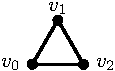
\includegraphics[height=5ex]{figures/triangleSimplizialkomplex.pdf}}}
%    \textbf{Bew.:} $S^1$ ist homöomorph zum Simplizialkomplex 
%                   $X = \triangleSimplizialkomplex$, d.~h. dem Rand
%                   von $\Delta^2$. Es gilt:
%            \[X = \Set{\underbrace{v_0, v_1, v_2}_{A_0(X)}, \underbrace{\Delta (v_1, v_2)}_{=: a_0}, \underbrace{\underbrace{\Delta (v_0, v_2)}_{=: a_1}, \underbrace{\Delta(v_0, v_1)}_{=: a_2}}_{A_1(X)}}\]
%            Damit folgt: 
%        \begin{enumerate}
%            \item Für $k \geq 2$ ist $C_k(X) \cong 0$, da es in diesen 
%                Dimensionen keine Simplizes gibt, d.~h. $A_k(X) = \emptyset$ gilt.\\
%                Also: $H_k(X) \cong 0 \; \forall k \geq 2$
%            \item $C_0(X) = \Set{\sum_{i=0}^2 c_i v_i | c_i \in \mdr}$, da 
%                $A_0(x)$ Basis von $C_0(X)$ ist;\\
%                $C_1(X) = \Set{\sum_{i=0}^2 c_i a_i | c_i \in \mdr}$, da 
%                $A_1(X)$ Basis von $C_1(X)$ ist.
%            \item Für die Randabbildungen $d_i: C_i(X) \rightarrow C_{i-1}(X)$ gilt:
%                $d_0 \equiv 0$, $d_1: C_1(X) \rightarrow C_0(X)$ ist definiert durch
%                $d_1(a_k) = \sum_{i=0}^1 (-1)^i \partial_i(a_k) = \partial_0 (a_k) - \partial_1(a_k) \; \forall k \in \Set{0,1,2}$
%        \end{enumerate}
%\end{solution}

%Auch diese Aufgabe ist zu lang
%\begin{solution}[\ref{ub7:aufg3}]
%
%\end{solution}

\begin{solution}[\ref{ub11:aufg3}]
    \textbf{Vor.:} Sei $(X, d)$ eine absolute Ebene, $A, B, C \in X$
        und $\triangle ABC$ ein Dreieck.

    \begin{enumerate}[label=(\alph*)]
        \item \textbf{Beh.:} $\overline{AB} \cong \overline{AC} \Rightarrow \angle ABC \cong \angle ACB$\\
              \textbf{Bew.:} Sei $\overline{AB} \cong \overline{AC}$.\\
              $\Rightarrow \exists$ Isometrie $\varphi$ mit $\varphi(B) = C$ und
              $\varphi(C) = B$ und $\varphi(A) = A$.\\
              $\Rightarrow \varphi(\angle ABC) = \angle ACB$\\
              $\Rightarrow \angle ABC \cong \angle ACB \qed$
        \item \textbf{Beh.:} Der längeren Seite von $\triangle ABC$ liegt der größere Winkel gegenüber und
              umgekehrt.\\
              \textbf{Bew.:} Sei $d(A,C) > d(A,B)$. Nach \ref{axiom:3.1}
              gibt es $C' \in AC^+$ mit $d(A, C') = d(A,B)$\\
              $\Rightarrow C'$ liegt zwischen $A$ und $C$.\\
              Es gilt $\measuredangle ABC' < \measuredangle ABC$ und
              aus \cref{ub11:aufg3.a} folgt: $\measuredangle ABC' = \measuredangle AC' B$.\\
              $\angle BC' A$ ist ein nicht anliegender Außenwinkel zu
              $\angle BCA \xRightarrow{\crefabbr{bem:14.9}} \measuredangle BC' A > \measuredangle BCA$\\
              $\Rightarrow \measuredangle BCA < \measuredangle BC' A = \measuredangle ABC' < \measuredangle ABC $
              Sei umgekehrt $\measuredangle ABC > \measuredangle BCA$,
              kann wegen 1. Teil von \cref{ub11:aufg3.b} nicht 
              $d(A,B) > d(A,C)$ gelten.\\
              Wegen \cref{ub11:aufg3.a} kann nicht $d(A,B) = d(A,C)$
              gelten.\\
              $\Rightarrow d(A,B) < d(A, C) \qed$
        \item \textbf{Vor.:} Sei $g$ eine Gerade, $P \in X$ und $P \notin g$\\
              \textbf{Beh.:} $\exists!$ Lot\\
              \textbf{Bew.:} ÜB10 A4(a): Es gibt Geradenspiegelung $\varphi$
              an $g$. $\varphi$ vertauscht die beiden Halbebenen bzgl.
              $g$.\\
              $\Rightarrow \varphi(P)P$ schneidet $g$ in $F$.

              %Nach ÜB 10 A4(a):
              Es gibt eine Geradenspiegelung $\varphi$ an $g$.
              $\varphi$ vertauscht die beiden Halbebenen bzgl. $g$
              $\Rightarrow \varphi(P)P$ schneidet $g$ in $F$.

              Sei $A \in g \setminus \Set{F}$. Dann gilt $\varphi(\angle AFP) = \angle AF \varphi(P) = \pi$
              $\Rightarrow \angle AFP$ ist rechter Winkel.

              Gäbe es nun $G \in g \setminus \Set{F}$, so dass $PG$ weiteres Lot von $P$ auf $g$ ist,
              wäre $\triangle PFG$ ein Dreieck mit zwei rechten Innenwinkeln (vgl. \cref{fig:two-perpendiculars}).

              \begin{figure}[htp]
                  \centering
                  \documentclass[varwidth=true, border=2pt]{standalone}
\usepackage{tkz-euclide}

\begin{document}
\usetkzobj{all}
\begin{tikzpicture}
    \tkzSetUpPoint[shape=circle,size=10,color=black,fill=black]
    \tkzSetUpLine[line width=1]
    \tkzDefPoints{0/3/A, 4/0/B, 3/3/P, 3/0.75/G}
    \tkzDefLine[perpendicular=through P,/tikz/overlay](A,B)\tkzGetPoint{x}
    \tkzInterLL(A,B)(P,x) \tkzGetPoint{F}

    \tkzMarkAngle[arc=l,size=0.4cm,color=red,fill=red!20](B,F,P)
    \tkzLabelAngle[pos = 0.2](B,F,P){$\cdot$}

    \tkzMarkAngle[arc=l,size=0.4cm,color=red,fill=red!20](P,G,A)
    \tkzLabelAngle[pos = 0.2](P,G,A){$\cdot$}

    \tkzDrawPoints(A,F,P,G)


    \tkzDrawSegments(A,B)
    \tkzDrawLines(A,B)
    \tkzDrawLine[dashed,color=orange,add=0.5 and 0.2](F,P)
    \tkzDrawLine[dashed,color=blue,add=0.5 and 0.2](G,P)
    % 
    \tkzLabelPoint[below left](A){$A$}
    \tkzLabelPoint[below left](G){$G$}
    \tkzLabelPoint[above left](P){$P$}
    \tkzLabelPoint[left](F){$F$}
    \tkzLabelLine[below,pos=1](A,B){$g$}
\end{tikzpicture}
\end{document}

                  \caption{Zwei Lote zu einer Geraden $g$ durch einen Punkt $P$}
                  \label{fig:two-perpendiculars}
              \end{figure}

              Nach \cref{folgerung:14.10} ist die Summe von zwei Innenwinkeln immer $< \pi$\\
              $\Rightarrow G$ gibt es nicht. $\qed$
    \end{enumerate}
\end{solution}

\begin{solution}[\ref{ub-tut-24:a1}]
    Sei $f \parallel h$ und \obda $f \parallel g$.

    $f \nparallel h \Rightarrow f \cap h \neq \emptyset$, sei also $x \in f \cap h$.
    Mit Axiom \ref{axiom:5} folgt: Es gibt höchstens eine Parallele
    zu $g$ durch $x$, da $x \notin g$. Diese ist $f$, da $x \in f$
    und $f \parallel g$. Da aber $x \in h$, kann $h$ nicht parallel
    zu $g$ sein, denn ansonsten gäbe es zwei Parallelen zu $g$ durch
    $x$ ($f \neq h$).
    $\Rightarrow g \nparallel h$ $\qed$
\end{solution}

\begin{solution}[\ref{ub-tut-24:a3}]
    Seien $\triangle ABC$ und $\triangle AB' C'$ Dreiecke mit
    \begin{align*}
        d(A, B)  &= d(A', B')\\
        d(B, C)  &= d(B', C')\\
        d(C, A)  &= d(C', A')
    \end{align*}

    Dann existiert nach \ref{axiom:4} genau eine Isometrie $\varphi$
    mit $\varphi(A) = A', \varphi(B) = B'$ und $\varphi(C) \in A' B' C'^+$.

    Da $d(A',C') = d(A,C) = d(\varphi(A), \varphi(C)) = d(A', \varphi(C))$
    und $d(B', C') = d(B', \varphi(C))$
    \todo[inline]{Da fehlt was.}
\end{solution}

\appendix
\chapter*{Bildquellen\markboth{Bildquellen}{Bildquellen}}
\addcontentsline{toc}{chapter}{Bildquellen}

Alle Bilder, die hier nicht aufgeführt sind, wurden selbst erstellt.

Teilweise wurden die im folgenden aufgelisteten Bilder noch leicht
modifiziert.

\begin{itemize}
    \item[Abb. \ref{fig:s2}] $S^2$: Tom Bombadil, \href{http://tex.stackexchange.com/a/42865/5645}{tex.stackexchange.com/a/42865}
    \item[Abb. \ref{fig:cube}] Würfel: Jan Hlavacek, \href{http://tex.stackexchange.com/a/12069/5645}{tex.stackexchange.com/a/12069}
    \item[Abb. \ref{fig:torus}] $T^2$: Jake, \href{http://tex.stackexchange.com/a/70979/5645}{tex.stackexchange.com/a/70979/5645}
    \item[Abb. \ref{fig:stereographic-projection}] Stereographische Projektion: \href{http://texample.net/tikz/examples/map-projections/}{texample.net/tikz/examples/map-projections}
    \item[Abb. \ref{fig:Knoten}] Knoten von Jim.belk aus der \enquote{\href{https://commons.wikimedia.org/wiki/Category:Blue_knots}{Blue knots}}-Serie:
        \begin{itemize}
            \item Trivialer Knoten: \href{https://commons.wikimedia.org/wiki/File:Blue_Unknot.png}{\path{commons.wikimedia.org/wiki/File:Blue_Unknot.png}}
            \item Kleeblattknoten: \href{https://commons.wikimedia.org/wiki/File:Blue_Trefoil_Knot.png}{\path{commons.wikimedia.org/wiki/File:Blue_Trefoil_Knot.png}}
            \item Achterknoten: \href{https://commons.wikimedia.org/wiki/File:Blue_Figure-Eight_Knot.png}{\path{commons.wikimedia.org/wiki/File:Blue_Figure-Eight_Knot.png}}
            \item $6_2$-Knoten: \href{https://commons.wikimedia.org/wiki/File:Blue_6_2_Knot.png}{\path{commons.wikimedia.org/wiki/File:Blue_6_2_Knot.png}}
        \end{itemize}
    \item[Abb. \ref{fig:reidemeister-zuege}] Reidemeister-Züge: YAMASHITA Makoto (\href{https://commons.wikimedia.org/wiki/File:Reidemeister_move_1.png}{1}, \href{https://commons.wikimedia.org/wiki/File:Reidemeister_move_1.png}{2}, \href{https://commons.wikimedia.org/wiki/File:Reidemeister_move_1.png}{3})
    \item[Abb. \ref{fig:treefoil-knot-three-colors}] Kleeblattknoten, 3-Färbung: Jim.belk, \href{https://commons.wikimedia.org/wiki/File:Tricoloring.png}{\path{commons.wikimedia.org/wiki/File:Tricoloring.png}}
    \item[Abb. \ref{fig:double-torus}] Doppeltorus: Oleg Alexandrov, \href{https://commons.wikimedia.org/wiki/File:Double_torus_illustration.png}{\path{commons.wikimedia.org/wiki/File:Double\_torus\_illustration.png}}
    \item[Abb. \ref{fig:faltungsdiagramm}] Faltungsdiagramm: Jérôme Urhausen, Email vom 11.02.2014.
    \item[Abb. \ref{fig:torus-three-paths}] 3 Pfade auf Torus: \href{http://tex.stackexchange.com/users/484/charles-staats}{Charles Staats}, \href{http://tex.stackexchange.com/a/149991/5645}{\path{tex.stackexchange.com/a/149991/5645}}
    \item[Abb. \ref{fig:ueberlappung-r1-spirale-s1}] Überlagerung von $S^1$ mit $\mdr$: \href{http://tex.stackexchange.com/users/22467/alex}{Alex}, \href{http://tex.stackexchange.com/a/149706/5645}{\path{tex.stackexchange.com/a/149706/5645}}
    \item[Abb. \ref{fig:bem:14.9}] Sphärisches Dreieck: \href{https://commons.wikimedia.org/wiki/User:DemonDeLuxe}{Dominique Toussaint},\\
        \href{https://commons.wikimedia.org/wiki/File:Spherical_triangle_3d_opti.png}{\path{commons.wikimedia.org/wiki/File:Spherical_triangle_3d_opti.png}}
    \item[Abb. \ref{fig:moebius-strip}] Möbiusband: \href{http://tex.stackexchange.com/users/2552/jake}{Jake},
        \href{http://tex.stackexchange.com/a/118573/5645}{\path{tex.stackexchange.com/a/118573/5645}}
\end{itemize}

\clearpage
%!TEX root = Programmierparadigmen.tex
\chapter*{Abkürzungsverzeichnis\markboth{Abkürzungsverzeichnis}{Abkürzungsverzeichnis}}
\addcontentsline{toc}{chapter}{Abkürzungsverzeichnis}
\begin{acronym}
    \acro{Beh.}{Behauptung}
    \acro{Bew.}{Beweis}
    \acro{bzgl.}{bezüglich}
    \acro{bzw.}{beziehungsweise}
    \acro{ca.}{circa}
    \acro{d. h.}{das heißt}
    \acro{DEA}{Deterministischer Endlicher Automat}
    \acro{etc.}{et cetera}
    \acro{ggf.}{gegebenenfalls}
    \acro{mgu}{most general unifier}
    \acro{sog.}{sogenannte}
    \acro{Vor.}{Voraussetzung}
    \acro{vgl.}{vergleiche}
    \acro{z. B.}{zum Beispiel}
    \acro{z. z.}{zu zeigen}
\end{acronym}

\clearpage
%!TEX root = GeoTopo.tex
\markboth{Anhang: Definitionen}{Anhang: Definitionen}
\chapter*{Anhang: Definitionen}
\addcontentsline{toc}{chapter}{Anhang: Definitionen}

Da dieses Skript in die Geometrie und Topologie einführen soll, sollten soweit
wie möglich alle benötigten Begriffe definiert und erklärt werden. Die folgenden
Begriffe wurden zwar verwendet, aber nicht erklärt, da sie Bestandteil der
Vorlesungen \enquote{Analysis I und II} sowie \enquote{Lineare Algebra und analytische Geometrie I und II}
sind. Jedoch will ich zumindest die Definitionen bereitstellen.

\begin{definition}\xindex{Häufungspunkt}
	Sei $D \subseteq \mdr$ und $x_0 \in \mdr$. $x_0$ heißt ein \textbf{Häufungspunkt}
	von $D :\gdw \exists$ Folge $x_n$ in $D \setminus \Set{x_0}$ mit $x_n \rightarrow x_0$.
\end{definition}

Folgende Definition wurde dem Skript von Herrn Prof. Dr. Leuzinger für
Lineare Algebra entnommen:

\begin{definition}\xindex{Abbildung!affine}
	Es seien $V$ und $W$ $\mdk$-Vektorräume und $\mda(V)$ und $\mda(W)$ die 
	zugehörigen affinen Räume. Eine Abbildung $f:V \rightarrow W$ heißt \textbf{affin},
	falls für alle $a, b \in V$ und alle $\lambda, \mu \in \mdk$ mit $\lambda + \mu = 1$ gilt:
	\[f(\lambda a + \mu b) = \lambda f(a) + \mu f(b)\]
\end{definition}

\begin{definition}\xindex{Orthonormalbasis}
	Sei $V$ ein Vektorraum und $S \subseteq V$ eine Teilmenge.

	$S$ heißt eine \textbf{Orthonormalbasis} von $V$, wenn gilt:
	\begin{defenumprops}
		\item $S$ ist eine Basis von $V$
		\item $\forall v \in S: \|v\| = 1$
		\item $\forall v_1, v_2 \in S: v_1 \neq v_2 \Rightarrow \langle v_1, v_2 \rangle = 0$
	\end{defenumprops}
\end{definition} 
\clearpage
%%%%%%%%%%%%%%%%%%%%%%%%%%%%%%%%%%%%%%%%%%%%%%%%%%%%%%%%%%%%%%%%%%%%%%
% Begriffslexikon zur Beschreibung des Produkts						 %
%%%%%%%%%%%%%%%%%%%%%%%%%%%%%%%%%%%%%%%%%%%%%%%%%%%%%%%%%%%%%%%%%%%%%%
%\newglossaryentry{sortierschluessel}
%{
%  name=Sortierschlüssel,
%  description={ein Schlüssel, anhand dessen diese Einträge sortiert werden}
%}
%\newacronym{abc}{Blub}{Bananarama}

%%%%%%%%%%%%%%%%%%%%%%%%%%%%%%%%%%%%%%%%%%%%%%%%%%%%%%%%%%%%%%%%%%%%%
% Mengenoperationen                                                 %
%%%%%%%%%%%%%%%%%%%%%%%%%%%%%%%%%%%%%%%%%%%%%%%%%%%%%%%%%%%%%%%%%%%%%
\newglossaryentry{Potenzmenge}
{
  name={\ensuremath{\mathcal{P}(M)}},
  description={Potenzmenge von $M$},
  sort=MengenoperationNPotenzmenge
}

\newglossaryentry{Abschluss}
{
  name={\ensuremath{\overline{M}}},
  description={Abschluss der Menge $M$},
  sort=MengenoperationFAbschluss
}

\newglossaryentry{Rand}
{
  name={\ensuremath{\partial M}},
  description={Rand der Menge $M$},
  sort=MengenoperationFRand
}

\newglossaryentry{Inneres}
{
  name={\ensuremath{M^\circ}},
  description={Inneres der Menge $M$},
  sort=MengenoperationFInneres
}

\newglossaryentry{Kreuzprodukt}
{
  name={\ensuremath{A \times B}},
  description={Kreuzprodukt zweier Mengen},
  sort=MengenoperationNKreuzprodukt
}
\newglossaryentry{subseteq}
{
  name={\ensuremath{A \subseteq B}},
  description={Teilmengenbeziehung},
  sort=MengenoperationNSubseteq
}
\newglossaryentry{subsetneq}
{
  name={\ensuremath{A \subsetneq B}},
  description={echte Teilmengenbeziehung},
  sort=MengenoperationNSubsetneq
}

\newglossaryentry{setminus}
{
  name={\ensuremath{A \setminus B}},
  description={$A$ ohne $B$},
  sort=MengenoperationNSetminus
}

%%%%%%%%%%%%%%%%%%%%%%%%%%%%%%%%%%%%%%%%%%%%%%%%%%%%%%%%%%%%%%%%%%%%%
% Zahlenmengen                                                      %
%%%%%%%%%%%%%%%%%%%%%%%%%%%%%%%%%%%%%%%%%%%%%%%%%%%%%%%%%%%%%%%%%%%%%

\newglossaryentry{Z}
{
  name={\ensuremath{\mdz}},
  description={Ganze Zahlen},
  sort=KoerperAZ
}

\newglossaryentry{Q}
{
  name={\ensuremath{\mdq}},
  description={Rationale Zahlen},
  sort=KoerperBQ
}

\newglossaryentry{R}
{
  name={\ensuremath{\mdr}},
  description={Reele Zahlen},
  sort=KoerperR
}

\newglossaryentry{Rplus}
{
  name={\ensuremath{\mdr^+}},
  description={Echt positive reele Zahlen},
  sort=KoerperRplus
}

\newglossaryentry{Einheitengruppe}
{
  name={\ensuremath{\mdr^\times}},
  description={Multiplikative Einheitengruppe von $\mdr$},
  sort=KoerperREinheiten
}

\newglossaryentry{Projektion}
{
  name={\ensuremath{\mathbb{P}}},
  description={Projektion},
  sort=KoerperXProjektion
}
%%%%%%%%%%%%%%%%%%%%%%%%%%%%%%%%%%%%%%%%%%%%%%%%%%%%%%%%%%%%%%%%%%%%%
% Sonstiges                                                         %
%%%%%%%%%%%%%%%%%%%%%%%%%%%%%%%%%%%%%%%%%%%%%%%%%%%%%%%%%%%%%%%%%%%%%
\newglossaryentry{Skalarprodukt}
{
  name={\ensuremath{\langle \cdot , \cdot \rangle}},
  description={Skalarprodukt},
  sort=ZZZSkalarprodukt
}

\newglossaryentry{Modulo}
{
  name={\ensuremath{X /_\sim}},
  description={$X$ modulo $\sim$},
  sort=ZZZAuequivalenzModulo
}

\newglossaryentry{Modulo-Aequivalenzklasse}
{
  name={\ensuremath{[x]_\sim}},
  description={Äquivalenzklassen von $x$ bzgl. $\sim$},
  sort=ZZZAuequivalenzKlassen
}

\newglossaryentry{Norm}
{
  name={\ensuremath{\| x \|}},
  description={Norm von $x$},
  sort=ZZZNorm
}

\newglossaryentry{Betrag}
{
  name={\ensuremath{| x |}},
  description={Betrag von $x$},
  sort=ZZZNormBetrag
}
%%%%%%%%%%%%%%%%%%%%%%%%%%%%%%%%%%%%%%%%%%%%%%%%%%%%%%%%%%%%%%%%%%%%%
% Fraktale Symbole                                                  %
%%%%%%%%%%%%%%%%%%%%%%%%%%%%%%%%%%%%%%%%%%%%%%%%%%%%%%%%%%%%%%%%%%%%%
\newglossaryentry{fB}
{
  name={\ensuremath{\fB}},
  description={Basis einer Topologie},
  sort=fB
}

\newglossaryentry{Epsilonumgebung}
{
  name={\ensuremath{\fB_\varepsilon(x)}},
  description={Offene Kugel mit Radius $\varepsilon$ um $x$ ($\varepsilon$-Umgebung)},
  sort=fBr
}

\newglossaryentry{fT}
{
  name={\ensuremath{\fT}},
  description={Topologie},
  sort=fT
}


% Setze den richtigen Namen für das Glossar
\renewcommand*{\glossaryname}{\glossarName}
\deftranslation{Glossary}{\glossarName}

% Drucke das gesamte Glossar
\glsaddall
\printglossaries

% Trage das Glossar in das Inhaltsverzeichnis ein
%\stepcounter{section}
%\addcontentsline{toc}{section}{\numberline {\thesection} \glossarName}
 
\clearpage
\addcontentsline{toc}{chapter}{Stichwortverzeichnis}
\renewcommand{\indexname}{Stichwortverzeichnis}
\printindex
\end{document}
